% Options for packages loaded elsewhere
% Options for packages loaded elsewhere
\PassOptionsToPackage{unicode}{hyperref}
\PassOptionsToPackage{hyphens}{url}
\PassOptionsToPackage{dvipsnames,svgnames,x11names}{xcolor}
%
\documentclass[
  letterpaper,
  DIV=11,
  numbers=noendperiod]{scrreprt}
\usepackage{xcolor}
\usepackage{amsmath,amssymb}
\setcounter{secnumdepth}{5}
\usepackage{iftex}
\ifPDFTeX
  \usepackage[T1]{fontenc}
  \usepackage[utf8]{inputenc}
  \usepackage{textcomp} % provide euro and other symbols
\else % if luatex or xetex
  \usepackage{unicode-math} % this also loads fontspec
  \defaultfontfeatures{Scale=MatchLowercase}
  \defaultfontfeatures[\rmfamily]{Ligatures=TeX,Scale=1}
\fi
\usepackage{lmodern}
\ifPDFTeX\else
  % xetex/luatex font selection
\fi
% Use upquote if available, for straight quotes in verbatim environments
\IfFileExists{upquote.sty}{\usepackage{upquote}}{}
\IfFileExists{microtype.sty}{% use microtype if available
  \usepackage[]{microtype}
  \UseMicrotypeSet[protrusion]{basicmath} % disable protrusion for tt fonts
}{}
\makeatletter
\@ifundefined{KOMAClassName}{% if non-KOMA class
  \IfFileExists{parskip.sty}{%
    \usepackage{parskip}
  }{% else
    \setlength{\parindent}{0pt}
    \setlength{\parskip}{6pt plus 2pt minus 1pt}}
}{% if KOMA class
  \KOMAoptions{parskip=half}}
\makeatother
% Make \paragraph and \subparagraph free-standing
\makeatletter
\ifx\paragraph\undefined\else
  \let\oldparagraph\paragraph
  \renewcommand{\paragraph}{
    \@ifstar
      \xxxParagraphStar
      \xxxParagraphNoStar
  }
  \newcommand{\xxxParagraphStar}[1]{\oldparagraph*{#1}\mbox{}}
  \newcommand{\xxxParagraphNoStar}[1]{\oldparagraph{#1}\mbox{}}
\fi
\ifx\subparagraph\undefined\else
  \let\oldsubparagraph\subparagraph
  \renewcommand{\subparagraph}{
    \@ifstar
      \xxxSubParagraphStar
      \xxxSubParagraphNoStar
  }
  \newcommand{\xxxSubParagraphStar}[1]{\oldsubparagraph*{#1}\mbox{}}
  \newcommand{\xxxSubParagraphNoStar}[1]{\oldsubparagraph{#1}\mbox{}}
\fi
\makeatother

\usepackage{color}
\usepackage{fancyvrb}
\newcommand{\VerbBar}{|}
\newcommand{\VERB}{\Verb[commandchars=\\\{\}]}
\DefineVerbatimEnvironment{Highlighting}{Verbatim}{commandchars=\\\{\}}
% Add ',fontsize=\small' for more characters per line
\usepackage{framed}
\definecolor{shadecolor}{RGB}{241,243,245}
\newenvironment{Shaded}{\begin{snugshade}}{\end{snugshade}}
\newcommand{\AlertTok}[1]{\textcolor[rgb]{0.68,0.00,0.00}{#1}}
\newcommand{\AnnotationTok}[1]{\textcolor[rgb]{0.37,0.37,0.37}{#1}}
\newcommand{\AttributeTok}[1]{\textcolor[rgb]{0.40,0.45,0.13}{#1}}
\newcommand{\BaseNTok}[1]{\textcolor[rgb]{0.68,0.00,0.00}{#1}}
\newcommand{\BuiltInTok}[1]{\textcolor[rgb]{0.00,0.23,0.31}{#1}}
\newcommand{\CharTok}[1]{\textcolor[rgb]{0.13,0.47,0.30}{#1}}
\newcommand{\CommentTok}[1]{\textcolor[rgb]{0.37,0.37,0.37}{#1}}
\newcommand{\CommentVarTok}[1]{\textcolor[rgb]{0.37,0.37,0.37}{\textit{#1}}}
\newcommand{\ConstantTok}[1]{\textcolor[rgb]{0.56,0.35,0.01}{#1}}
\newcommand{\ControlFlowTok}[1]{\textcolor[rgb]{0.00,0.23,0.31}{\textbf{#1}}}
\newcommand{\DataTypeTok}[1]{\textcolor[rgb]{0.68,0.00,0.00}{#1}}
\newcommand{\DecValTok}[1]{\textcolor[rgb]{0.68,0.00,0.00}{#1}}
\newcommand{\DocumentationTok}[1]{\textcolor[rgb]{0.37,0.37,0.37}{\textit{#1}}}
\newcommand{\ErrorTok}[1]{\textcolor[rgb]{0.68,0.00,0.00}{#1}}
\newcommand{\ExtensionTok}[1]{\textcolor[rgb]{0.00,0.23,0.31}{#1}}
\newcommand{\FloatTok}[1]{\textcolor[rgb]{0.68,0.00,0.00}{#1}}
\newcommand{\FunctionTok}[1]{\textcolor[rgb]{0.28,0.35,0.67}{#1}}
\newcommand{\ImportTok}[1]{\textcolor[rgb]{0.00,0.46,0.62}{#1}}
\newcommand{\InformationTok}[1]{\textcolor[rgb]{0.37,0.37,0.37}{#1}}
\newcommand{\KeywordTok}[1]{\textcolor[rgb]{0.00,0.23,0.31}{\textbf{#1}}}
\newcommand{\NormalTok}[1]{\textcolor[rgb]{0.00,0.23,0.31}{#1}}
\newcommand{\OperatorTok}[1]{\textcolor[rgb]{0.37,0.37,0.37}{#1}}
\newcommand{\OtherTok}[1]{\textcolor[rgb]{0.00,0.23,0.31}{#1}}
\newcommand{\PreprocessorTok}[1]{\textcolor[rgb]{0.68,0.00,0.00}{#1}}
\newcommand{\RegionMarkerTok}[1]{\textcolor[rgb]{0.00,0.23,0.31}{#1}}
\newcommand{\SpecialCharTok}[1]{\textcolor[rgb]{0.37,0.37,0.37}{#1}}
\newcommand{\SpecialStringTok}[1]{\textcolor[rgb]{0.13,0.47,0.30}{#1}}
\newcommand{\StringTok}[1]{\textcolor[rgb]{0.13,0.47,0.30}{#1}}
\newcommand{\VariableTok}[1]{\textcolor[rgb]{0.07,0.07,0.07}{#1}}
\newcommand{\VerbatimStringTok}[1]{\textcolor[rgb]{0.13,0.47,0.30}{#1}}
\newcommand{\WarningTok}[1]{\textcolor[rgb]{0.37,0.37,0.37}{\textit{#1}}}

\usepackage{longtable,booktabs,array}
\usepackage{calc} % for calculating minipage widths
% Correct order of tables after \paragraph or \subparagraph
\usepackage{etoolbox}
\makeatletter
\patchcmd\longtable{\par}{\if@noskipsec\mbox{}\fi\par}{}{}
\makeatother
% Allow footnotes in longtable head/foot
\IfFileExists{footnotehyper.sty}{\usepackage{footnotehyper}}{\usepackage{footnote}}
\makesavenoteenv{longtable}
\usepackage{graphicx}
\makeatletter
\newsavebox\pandoc@box
\newcommand*\pandocbounded[1]{% scales image to fit in text height/width
  \sbox\pandoc@box{#1}%
  \Gscale@div\@tempa{\textheight}{\dimexpr\ht\pandoc@box+\dp\pandoc@box\relax}%
  \Gscale@div\@tempb{\linewidth}{\wd\pandoc@box}%
  \ifdim\@tempb\p@<\@tempa\p@\let\@tempa\@tempb\fi% select the smaller of both
  \ifdim\@tempa\p@<\p@\scalebox{\@tempa}{\usebox\pandoc@box}%
  \else\usebox{\pandoc@box}%
  \fi%
}
% Set default figure placement to htbp
\def\fps@figure{htbp}
\makeatother


% definitions for citeproc citations
\NewDocumentCommand\citeproctext{}{}
\NewDocumentCommand\citeproc{mm}{%
  \begingroup\def\citeproctext{#2}\cite{#1}\endgroup}
\makeatletter
 % allow citations to break across lines
 \let\@cite@ofmt\@firstofone
 % avoid brackets around text for \cite:
 \def\@biblabel#1{}
 \def\@cite#1#2{{#1\if@tempswa , #2\fi}}
\makeatother
\newlength{\cslhangindent}
\setlength{\cslhangindent}{1.5em}
\newlength{\csllabelwidth}
\setlength{\csllabelwidth}{3em}
\newenvironment{CSLReferences}[2] % #1 hanging-indent, #2 entry-spacing
 {\begin{list}{}{%
  \setlength{\itemindent}{0pt}
  \setlength{\leftmargin}{0pt}
  \setlength{\parsep}{0pt}
  % turn on hanging indent if param 1 is 1
  \ifodd #1
   \setlength{\leftmargin}{\cslhangindent}
   \setlength{\itemindent}{-1\cslhangindent}
  \fi
  % set entry spacing
  \setlength{\itemsep}{#2\baselineskip}}}
 {\end{list}}
\usepackage{calc}
\newcommand{\CSLBlock}[1]{\hfill\break\parbox[t]{\linewidth}{\strut\ignorespaces#1\strut}}
\newcommand{\CSLLeftMargin}[1]{\parbox[t]{\csllabelwidth}{\strut#1\strut}}
\newcommand{\CSLRightInline}[1]{\parbox[t]{\linewidth - \csllabelwidth}{\strut#1\strut}}
\newcommand{\CSLIndent}[1]{\hspace{\cslhangindent}#1}



\setlength{\emergencystretch}{3em} % prevent overfull lines

\providecommand{\tightlist}{%
  \setlength{\itemsep}{0pt}\setlength{\parskip}{0pt}}



 


\KOMAoption{captions}{tableheading}
\makeatletter
\@ifpackageloaded{tcolorbox}{}{\usepackage[skins,breakable]{tcolorbox}}
\@ifpackageloaded{fontawesome5}{}{\usepackage{fontawesome5}}
\definecolor{quarto-callout-color}{HTML}{909090}
\definecolor{quarto-callout-note-color}{HTML}{0758E5}
\definecolor{quarto-callout-important-color}{HTML}{CC1914}
\definecolor{quarto-callout-warning-color}{HTML}{EB9113}
\definecolor{quarto-callout-tip-color}{HTML}{00A047}
\definecolor{quarto-callout-caution-color}{HTML}{FC5300}
\definecolor{quarto-callout-color-frame}{HTML}{acacac}
\definecolor{quarto-callout-note-color-frame}{HTML}{4582ec}
\definecolor{quarto-callout-important-color-frame}{HTML}{d9534f}
\definecolor{quarto-callout-warning-color-frame}{HTML}{f0ad4e}
\definecolor{quarto-callout-tip-color-frame}{HTML}{02b875}
\definecolor{quarto-callout-caution-color-frame}{HTML}{fd7e14}
\makeatother
\makeatletter
\@ifpackageloaded{bookmark}{}{\usepackage{bookmark}}
\makeatother
\makeatletter
\@ifpackageloaded{caption}{}{\usepackage{caption}}
\AtBeginDocument{%
\ifdefined\contentsname
  \renewcommand*\contentsname{Table of contents}
\else
  \newcommand\contentsname{Table of contents}
\fi
\ifdefined\listfigurename
  \renewcommand*\listfigurename{List of Figures}
\else
  \newcommand\listfigurename{List of Figures}
\fi
\ifdefined\listtablename
  \renewcommand*\listtablename{List of Tables}
\else
  \newcommand\listtablename{List of Tables}
\fi
\ifdefined\figurename
  \renewcommand*\figurename{Figure}
\else
  \newcommand\figurename{Figure}
\fi
\ifdefined\tablename
  \renewcommand*\tablename{Table}
\else
  \newcommand\tablename{Table}
\fi
}
\@ifpackageloaded{float}{}{\usepackage{float}}
\floatstyle{ruled}
\@ifundefined{c@chapter}{\newfloat{codelisting}{h}{lop}}{\newfloat{codelisting}{h}{lop}[chapter]}
\floatname{codelisting}{Listing}
\newcommand*\listoflistings{\listof{codelisting}{List of Listings}}
\makeatother
\makeatletter
\makeatother
\makeatletter
\@ifpackageloaded{caption}{}{\usepackage{caption}}
\@ifpackageloaded{subcaption}{}{\usepackage{subcaption}}
\makeatother
\usepackage{bookmark}
\IfFileExists{xurl.sty}{\usepackage{xurl}}{} % add URL line breaks if available
\urlstyle{same}
\hypersetup{
  pdftitle={Basic Ecological Concepts and Data in R},
  pdfauthor={Dr.~Hank Stevens},
  colorlinks=true,
  linkcolor={blue},
  filecolor={Maroon},
  citecolor={Blue},
  urlcolor={Blue},
  pdfcreator={LaTeX via pandoc}}


\title{Basic Ecological Concepts and Data in R}
\author{Dr.~Hank Stevens}
\date{2026-06-03}
\begin{document}
\maketitle

\renewcommand*\contentsname{Table of contents}
{
\hypersetup{linkcolor=}
\setcounter{tocdepth}{2}
\tableofcontents
}

\bookmarksetup{startatroot}

\chapter*{Preface}\label{preface}
\addcontentsline{toc}{chapter}{Preface}

\markboth{Preface}{Preface}

This book provides an activity-based approach introduction to the
science and practice of ecology. It is designed to form the basis of an
undergraduate general ecology course. It includes real-world assessment
activities, and so answer keys are not generally available, even if they
might be appropriate in some situations.

Each chapter provides,

\begin{itemize}
\tightlist
\item
  links to background information in the form of a video lecture,
  peer-reviewed publications, and sometimes other sources,
\item
  one or more writing assignments, and
\item
  data exploration and modeling.
\end{itemize}

Each chapter mixes (i) ecological content and (ii) coding practices.
Students will get the most out of the content if they understand and
\emph{accept} this from the start. Avoiding one or the other reduces
their ability to understand, appreciate, and use both.

\section*{Guidance}\label{guidance}
\addcontentsline{toc}{section}{Guidance}

\markright{Guidance}

Use these tips to help reduce frustration and make things work better:

\begin{itemize}
\tightlist
\item
  The book should be read and the code implemented in sequence. For
  example, you should complete chapter 1 before chapter 2, complete
  chapter 2 before chapter 3, and so on. That is for two reasons. First,
  you will learn things about R and your computer in earlier chapters
  that you may need to know for later chapters. This is especially true
  for the first few chapters. Second, you will gain ecological knowledge
  in earlier chapters that enrich your experience in later chapters.
\item
  When the text provides an enumerated list or \emph{numbered} bullet
  items (e.g., 1, 2, 3 or a, b, c), it is usually very important or even
  essential to do these steps in sequence. There will be times that it
  is impossible to succeed unless you do the steps in \emph{sequence}.
\item
  When the text provides a simple, unnumbered list, it is usually not
  important to consider these items as representing a sequence.
\item
  I included a few sections entitled \emph{Overthinking}. I stole this
  idea from Richard McElreath (McElreath 2020), and these are sections
  that you can skip on the first read, and are not essentially for
  getting things to \emph{work}. They provide deeper, more detailed
  explanations than is typically required.
\end{itemize}

\section*{Other books}\label{other-books}
\addcontentsline{toc}{section}{Other books}

\markright{Other books}

My other books include
\href{https://hankstevens.github.io/Primer-of-Ecology/}{\emph{A Primer
of Ecology using R}} and
\href{https://hankstevens.github.io/ecosystems-primer/}{\emph{A Primer
of Ecosystem Modeling}}. The former (Primer of Ecology) is designed
primarily for beginning graduate students as a primer to theory in
population and community ecology. It was first published with Springer
in 2009, and the current GitHub version is quite updated. I use the
latter (ecosystem modeling) when I co-instruct a graduate course led by
colleagues who are real ecosystem ecologists (Drs. Melany Fisk, Mike
Vanni, and Lesley Knoll).

\emph{Mazel tov!}

\bookmarksetup{startatroot}

\chapter{AI and the Changing Landscape of Skills in
Ecology}\label{sec-ai-skills}

\emph{What should you learn, when the machine already ``knows'' so
much?}

\section{Background}\label{background}

You are learning ecology at a moment when artificial intelligence can
write passable R code, summarize journal articles, and define terms like
``carrying capacity'' faster than you can open a textbook. That fact
changes what it means to be well-trained in ecology. It does not,
however, reduce the amount you need to learn --- it shifts \emph{what}
you need to learn.

This chapter is addressed to both students and instructors. Its goal is
to lay out a practical framework for thinking about which skills matter
more than ever in an era of large language models (LLMs) like Claude,
ChatGPT, and their successors, and which tasks can be responsibly shared
with these tools. We focus on quantitative ecology because that is what
this book is about, but the ideas extend broadly.

The central argument is this: \textbf{AI's fluency with ecological
language makes it \emph{more} important, not less, that you develop deep
understanding of ecological mechanisms, model assumptions, and data
interpretation.} A machine can generate a plausible-sounding paragraph
about density dependence in thirty seconds. Only a well-trained
ecologist can recognize when that paragraph is subtly wrong.

\section{A framework: durable skills vs.~AI-augmentable
tasks}\label{a-framework-durable-skills-vs.-ai-augmentable-tasks}

Not all skills are equally vulnerable to automation. A useful way to
think about your education is to distinguish between two categories.

\textbf{Durable human skills} are things that require biological
intuition, judgment under uncertainty, and the ability to connect
mathematical abstractions to the living world. These are hard-won, slow
to develop, and not reliably performed by current AI. They include:

\begin{itemize}
\tightlist
\item
  \emph{Ecological intuition} --- the ability to walk into a forest, a
  marsh, or a dataset and notice what is ecologically interesting or
  surprising.
\item
  \emph{Mechanistic reasoning} --- understanding \emph{why} a model
  behaves the way it does, not just \emph{that} it produces a particular
  output.
\item
  \emph{Mathematical reasoning} --- the ability to follow the formal
  logic of a derivation, so that you can verify results, understand why
  an equation predicts what it does, and catch errors that sound
  plausible but are wrong.
\item
  \emph{Model assumption literacy} --- knowing what a model assumes,
  when those assumptions are reasonable, and what happens when they are
  violated.
\item
  \emph{Data literacy} --- the judgment to know whether data are
  adequate to answer a question, what biases they carry, and what they
  cannot tell you.
\item
  \emph{Multi-scale synthesis} --- connecting processes at the scale of
  an individual organism to patterns at the scale of a landscape or a
  globe.
\end{itemize}

\textbf{AI-augmentable tasks} are things that AI tools can do reasonably
well right now, and will likely do better over time. These include:

\begin{itemize}
\tightlist
\item
  Summarizing the main findings of a journal article.
\item
  Generating boilerplate R code for standard analyses (e.g., fitting a
  linear model, making a scatterplot).
\item
  Looking up definitions of ecological terms.
\item
  Drafting outlines or initial structure for a written argument.
\item
  Translating between programming languages.
\end{itemize}

Here is the key insight: \textbf{AI-augmentable does not mean
unimportant.} You still need to understand what a linear model does and
why, even if you let an AI draft the code. The danger is not that AI
does these tasks --- it is that you might skip the understanding that
makes you capable of evaluating whether the AI did them
\emph{correctly.}

\section{Why AI makes ecological understanding more
important}\label{why-ai-makes-ecological-understanding-more-important}

This point deserves emphasis, because it is counterintuitive. You might
think: if AI can write my R code and summarize my readings, I can spend
less time on those things and more time on\ldots{} something else. But
consider what actually happens.

Suppose you ask an AI to write R code that simulates logistic population
growth. The AI will almost certainly produce something that runs. But
will it use the continuous-time or discrete-time model? Will it handle
the time lag that makes the discrete model capable of oscillations and
chaos? Will it set up the parameters in a biologically meaningful range?
If you do not know enough to answer these questions, you cannot evaluate
the code. You are flying blind.

Or suppose you ask an AI to explain why two competing species cannot
coexist indefinitely. The AI will probably give you something that
sounds like the competitive exclusion principle. But it might gloss over
the specific conditions required, or fail to mention that the principle
applies to a particular model with particular assumptions, and that real
communities are far more complicated. The explanation will \emph{sound}
right. Whether it \emph{is} right depends on what you, the human
ecologist, know.

\begin{tcolorbox}[enhanced jigsaw, toprule=.15mm, colframe=quarto-callout-important-color-frame, bottomrule=.15mm, arc=.35mm, breakable, leftrule=.75mm, rightrule=.15mm, bottomtitle=1mm, coltitle=black, left=2mm, titlerule=0mm, title=\textcolor{quarto-callout-important-color}{\faExclamation}\hspace{0.5em}{The Plausibility Trap}, toptitle=1mm, colbacktitle=quarto-callout-important-color!10!white, opacityback=0, colback=white, opacitybacktitle=0.6]

AI-generated text about ecology is often \emph{plausible but wrong} in
ways that require ecological training to detect. The better the AI gets
at sounding like an ecologist, the more you need to actually \emph{be}
one.

\end{tcolorbox}

This is what we call the \textbf{plausibility trap}. AI systems are
trained to produce text (and code) that looks like text (and code)
produced by experts. They are not trained to be correct about the
natural world. They have no field experience, no memory of watching a
population crash, no intuition about whether a parameter value makes
biological sense. They are pattern-matching engines --- powerful ones,
but without grounding in physical and biological reality.

\section{Six categories of skills to
develop}\label{six-categories-of-skills-to-develop}

Let us get specific. Below are six categories of durable skills, each
illustrated with examples from quantitative ecology. These are the
skills this textbook is designed to build, and the ones you should
invest in most heavily.

\subsection{1. Mechanistic reasoning}\label{mechanistic-reasoning}

Mechanistic reasoning is the ability to explain \emph{why} an ecological
pattern exists by tracing it back to underlying biological processes. It
is the difference between saying ``the population oscillates'' and
saying ``the population oscillates \emph{because} the discrete-time
logistic model builds in a one-generation time lag between when crowding
occurs and when its effects on reproduction are realized, and when \(r\)
is large enough, this lag causes the population to overshoot and
undershoot \(K\) repeatedly.''

AI can describe patterns. It can even parrot mechanistic explanations it
has seen in training data. What it cannot do reliably is generate
mechanistic reasoning about novel situations --- situations where you
are looking at a dataset or a model output that nobody has analyzed
before. That is what ecologists do.

\textbf{How to practice it.} Throughout this book, when you are asked to
run a simulation or examine data, \emph{always} ask yourself: \emph{Why
does this pattern exist? What mechanism produces it?} Do not settle for
describing what you see. Explain what causes it.

\subsection{2. Mathematical reasoning as ecological
understanding}\label{mathematical-reasoning-as-ecological-understanding}

Ecology uses mathematics to turn assumptions into predictions. When we
write \(dN/dt = rN(1 - \alpha N)\) and solve for equilibrium, we are not
doing math for its own sake --- we are asking ``what controls the
long-term fate of this population?'' and letting algebra answer the
question. The derivation \emph{is} the ecological reasoning, expressed
in a language precise enough to check.

Put simply: \textbf{mathematical reasoning is a form of ecological
understanding} --- not a prerequisite for it, not a supplement to it,
but one of the ways you actually come to understand how ecological
systems work. When a student derives \(K = 1/\alpha\) and grasps that
carrying capacity is the reciprocal of the per-capita competitive
effect, they have learned something about ecology that no amount of
reading prose --- whether written by a textbook or an AI --- will give
them. The derivation is not an obstacle on the way to understanding. It
\emph{is} the understanding.

This matters enormously in an AI era. An AI can solve
\(0 = rN(1 - \alpha N)\) and tell you \(N^* = 1/\alpha\). But can you
verify that? Can you see \emph{why} the equilibrium depends on
\(\alpha\) and not on \(r\)? Can you explain what that means
biologically --- that the long-term population size depends on how
strongly individuals affect each other, not on how fast they reproduce?
If you can follow the two lines of algebra, these insights are obvious.
If you cannot, you are taking the AI's word for it.

The same applies at every level of model complexity in this book. When
you derive the invasion criterion for two-species competition
(\(K_2 > \beta K_1\)), you are discovering --- through logic --- the
conditions under which a species can persist. When you estimate
predator-prey parameters from moose and wolf population data, you are
using the structure of an equation to extract biological meaning. These
are not exercises in calculation. They are exercises in understanding.

\textbf{The risk of skipping the math is not that you get a wrong
number. It is that you lose the ability to tell whether a number is
wrong.} An AI can produce an answer that looks right. Only someone who
can follow the formal logic can confirm that it \emph{is} right --- or
catch where it isn't.

\textbf{How to practice it.} When this book asks you to solve an
equation or work through a derivation, do not skip to the answer. Follow
each step and ask: \emph{what biological fact does this step reflect?}
When you reach the result, ask: \emph{which parameters appear, which
don't, and what does that tell me about what matters in this system?}

\subsection{3. Model assumption
literacy}\label{model-assumption-literacy}

Every ecological model is a set of assumptions about how the world
works. The exponential growth model assumes unlimited resources and no
density dependence. The logistic model assumes that per capita growth
rate declines linearly with population size. The Lotka-Volterra
competition model assumes that the effect of one competitor on another
is constant regardless of density.

These assumptions are not fine print. They are the \emph{substance} of
the model. When an assumption is violated, the model's predictions can
be wildly wrong. Understanding which assumptions matter and when they
might be violated is one of the most important skills in ecology.

\begin{tcolorbox}[enhanced jigsaw, toprule=.15mm, colframe=quarto-callout-tip-color-frame, bottomrule=.15mm, arc=.35mm, breakable, leftrule=.75mm, rightrule=.15mm, bottomtitle=1mm, coltitle=black, left=2mm, titlerule=0mm, title=\textcolor{quarto-callout-tip-color}{\faLightbulb}\hspace{0.5em}{A Useful Habit}, toptitle=1mm, colbacktitle=quarto-callout-tip-color!10!white, opacityback=0, colback=white, opacitybacktitle=0.6]

Before running any model, write down its key assumptions in your own
words. Then ask: \emph{Which of these assumptions could be wrong for the
system I am studying, and how would that change the predictions?}

\end{tcolorbox}

AI tools are particularly poor at this. They can list assumptions from a
textbook, but they cannot walk outside and check whether density
dependence in your study population really is linear, or whether the
competitive effect of species A on species B really is constant. That
judgment requires you.

\subsection{4. Prediction before
computation}\label{prediction-before-computation}

One of the most effective learning strategies in quantitative ecology is
to \emph{make a prediction before you run the code.} What do you think
will happen when you double the intrinsic growth rate? What do you
expect the graph to look like when you increase carrying capacity? What
will happen to coexistence if you make one species a much stronger
competitor?

If you write down your prediction and it turns out to be wrong, you have
learned something valuable: there is a gap between your mental model and
the mathematical model. That gap is where real understanding develops.

AI eliminates this step if you let it. You can ask an AI what will
happen, and it will tell you, and you will nod and move on without ever
experiencing the discomfort of being wrong. \emph{Resist this.} Your
mistakes are the raw material of learning.

\textbf{How to practice it.} Every time this textbook asks you to run a
simulation or modify a parameter, pause. Write down, in one sentence,
what you predict will happen and \emph{why.} Then run the code and
compare. If you were wrong, figure out why.

\subsection{5. Data literacy and
judgment}\label{data-literacy-and-judgment}

Data literacy goes beyond knowing how to make a scatterplot or compute a
mean. It includes:

\begin{itemize}
\tightlist
\item
  Recognizing what kinds of variation are present in a dataset
  (measurement error, natural variation, sampling bias).
\item
  Understanding what a dataset \emph{cannot} tell you because of how it
  was collected.
\item
  Knowing when a sample size is too small to support a conclusion.
\item
  Distinguishing correlation from causation with genuine understanding
  rather than just reciting the phrase.
\item
  Recognizing when an apparent pattern might be an artifact of how the
  data were processed.
\end{itemize}

These judgments are context-dependent and require understanding of both
the statistical tools and the biological system. AI can compute a
p-value, but it cannot tell you whether the study design that produced
the data makes that p-value meaningful.

\textbf{How to practice it.} When you encounter data in this book, do
not just analyze them. \emph{Interrogate} them. How were they collected?
What could go wrong? What alternative explanations exist for the
patterns you see?

\subsection{6. Multi-scale synthesis}\label{multi-scale-synthesis}

Ecology spans scales from molecules to the biosphere. A well-trained
ecologist can connect processes at different scales: how individual
behavior gives rise to population dynamics, how population dynamics
shape community composition, how community composition affects ecosystem
function.

This kind of synthesis requires holding multiple frameworks in your head
simultaneously and recognizing when processes at one scale constrain or
enable processes at another. AI can retrieve information about any one
of these scales, but it struggles to make the cross-scale connections
that produce genuine ecological insight.

\textbf{How to practice it.} As you move through this book from
individual ecology to population dynamics to community ecology to
ecosystems, keep asking: \emph{How does what I learned in earlier
chapters connect to what I am learning now?}

\section{Learn to distinguish between understanding and
doing}\label{learn-to-distinguish-between-understanding-and-doing}

Writing code that plots your data is different from writing code that
simulates density-dependent growth. The first you check by looking at
the plot --- did it do what I wanted? The second you check by
interrogating the assumptions you built into the model. This distinction
matters for how you think about AI and coding in this course.

Code that generates data displays, apps, or games is code that you check
primarily via output. You look at or use the output and ask, did the
code do what I wanted it to do? If not, attempt to troubleshoot and try
again.

In contrast, code that generates mechanistic and statistical models is
code that you have to understand and check primarily by evaluating
assumptions that you tried to manifest in your code.

Mechanistic models are simply tools to turn assumptions into
predictions, so you really need to understand how you are building those
assumptions.

The output of your mechanistic model constitutes your predictions. You
need to trust those predictions because they follow directly from the
assumptions that you made. If the predictions seem off to you, then you
need to reconsider the assumptions you made. There are three types of
situations to consider:

\begin{enumerate}
\def\labelenumi{\arabic{enumi}.}
\tightlist
\item
  \emph{Do you have a simple coding error}? Does your code do what you
  intended? E.g., did you use Boolean logic correctly, or create input
  to a function that merely wasn't in the right sequence?
\item
  \emph{Does your math match your ecology}? How you use mathematical
  functions to manifest your assumptions about the
  biological/ecological/physical features of the world can be tricky and
  problems fall into two buckets: sometimes the math doesn't do what you
  think it does, and other times the ecological assumptions have
  different consequences than you thought they would.

  \begin{enumerate}
  \def\labelenumii{\alph{enumii}.}
  \tightlist
  \item
    \emph{Are your mathematical assumptions correct}? There are some
    convenient mathematical operations and forms that you can collect in
    your toolbox: functions that put a ceiling or floor on values,
    functions that create positive feedback loops and negative feedback
    loops, functions that add and those that subtract; 0th, 1st, and 2nd
    order products of variables.
  \item
    \emph{Are your ecological assumptions correct}? This is the
    interesting situation, where your choices of mathematical functions
    or parameter estimates may or may not map onto reality.

    \begin{enumerate}
    \def\labelenumiii{\roman{enumiii}.}
    \tightlist
    \item
      If your ecological assumptions are wrong, that is great! You're
      learning something important about the world.
    \item
      If your ecological assumptions are correct but the outcome is
      unexpected, that is great --- you are discovering a consequence of
      your assumptions that your intuition hadn't predicted.
    \end{enumerate}
  \end{enumerate}
\end{enumerate}

This is where mathematical reasoning becomes your most important
verification tool. If an AI generates model code, you can check whether
it runs (easy) and whether the output looks reasonable (harder). But the
deepest check is whether the mathematical structure matches the biology
you intended. Does the code implement \(1 - N/K\) or \(1 - \alpha N\)?
Those are equivalent --- but only if \(\alpha = 1/K\). If you can't
follow that equivalence, you can't tell whether the AI's implementation
matches your biological intention. The formal logic is the bridge
between ``the code runs'' and ``the code is right.''

\textbf{How to practice it.} When you encounter a place in this book
where you need to use code, do not just copy some code nor ask AI for
it. Ask \emph{why am I writing code}?

\begin{enumerate}
\def\labelenumi{\arabic{enumi}.}
\tightlist
\item
  Is it to make a graph that displays data clearly?
\item
  Is it to use mathematics to represent some biological or physical
  process?
\item
  Is it to perform a statistical test in which I have to understand the
  assumptions of that test to apply it correctly?
\end{enumerate}

If you answer ``yes'' to no. 1, then using AI is \emph{relatively} safe,
but you can probably be most effective if you can work directly with any
code AI spits out for you.

If you answer ``yes'' to 2 or 3 above, then you really need to
understand what you are doing. You need to know \emph{not only} that two
cans of beer plus two cans of beer add up to four cans of beer, but what
will happen at the party once people start drinking it.

\section{Using AI responsibly in this
course}\label{using-ai-responsibly-in-this-course}

None of the above means you should avoid AI entirely. AI tools can be
genuinely useful in your ecological education, but they are useful in
the way a calculator is useful in a math course: they can save time on
mechanical tasks, but they cannot replace the thinking that makes the
tasks meaningful.

Here are some guidelines for responsible use.

\textbf{Good uses of AI in ecology coursework:}

\begin{itemize}
\tightlist
\item
  Debugging R code that throws an error you do not understand.
\item
  Getting a quick refresher on R syntax (e.g., ``How do I add a legend
  to a ggplot?'').
\item
  Generating a first draft of an outline that you then revise
  substantially.
\item
  Asking for alternative explanations of a concept you have already
  studied but find confusing.
\end{itemize}

\textbf{Risky uses of AI in ecology coursework:}

\begin{itemize}
\tightlist
\item
  Asking AI to explain an ecological concept you have not yet studied
  yourself. (You will not be able to evaluate the answer.)
\item
  Using AI-generated code without understanding every line of it.
\item
  Asking AI to interpret your results for you. (Interpretation requires
  the biological context that you, not the AI, possess.)
\item
  Asking AI to write your discussion or analysis. (This is where your
  own ecological thinking is supposed to develop.)
\end{itemize}

\begin{tcolorbox}[enhanced jigsaw, toprule=.15mm, colframe=quarto-callout-warning-color-frame, bottomrule=.15mm, arc=.35mm, breakable, leftrule=.75mm, rightrule=.15mm, bottomtitle=1mm, coltitle=black, left=2mm, titlerule=0mm, title=\textcolor{quarto-callout-warning-color}{\faExclamationTriangle}\hspace{0.5em}{The Code Comprehension Rule}, toptitle=1mm, colbacktitle=quarto-callout-warning-color!10!white, opacityback=0, colback=white, opacitybacktitle=0.6]

If you use AI to help write R code, you should be able to explain what
every line does and \emph{why} it is there. If you cannot, you have not
learned what you need to learn.

\end{tcolorbox}

\section{A note for instructors}\label{a-note-for-instructors}

If you are teaching with this book, the AI landscape is shifting under
your feet. Here are some principles that may help.

\textbf{Design assignments that require judgment, not just output.} If
an assignment can be completed by pasting the prompt into ChatGPT and
submitting the result, the assignment is testing the wrong thing.
Assignments should require students to make predictions, evaluate
assumptions, connect models to specific biological systems, and explain
\emph{why} a result makes ecological sense.

\textbf{Make AI use transparent, not forbidden.} Blanket bans on AI are
difficult to enforce and send the message that AI is cheating rather
than a tool. Instead, consider requiring students to document when and
how they used AI, and to reflect on what they learned (or failed to
learn) by using it. The goal is to develop students who can use AI
wisely, not students who can pretend they do not use it.

\textbf{Foreground assumptions explicitly.} When teaching any model,
spend time on what the model assumes and what would happen if those
assumptions were violated. Use callout boxes, discussion questions, and
activities that force students to engage with assumptions as substantive
ecological content, not as disclaimers to be skipped.

\textbf{Require prediction before computation.} Build the ``predict
first'' step into your workflow explicitly. Have students write
predictions in a worksheet, a shared document, or their lab notebooks
before they run code. This simple intervention creates the productive
struggle that drives learning.

\textbf{Use AI failures as teaching moments.} Ask an AI to explain an
ecological concept, and then have students identify what it got wrong.
This is a great exercise in critical thinking and assumption literacy
--- and it demonstrates, concretely, why human expertise matters.

\section{The skills that will define your
career}\label{the-skills-that-will-define-your-career}

The ecology profession is changing. Ecologists who graduate in the next
decade will work alongside AI tools that can process satellite imagery,
classify species from audio recordings, and generate code for complex
statistical analyses. The value of a human ecologist will not lie in
being able to do these things manually. It will lie in being able to:

\begin{itemize}
\tightlist
\item
  Ask the right questions about the natural world.
\item
  Design studies and models that can actually answer those questions.
\item
  Recognize when a tool (AI or otherwise) is giving you the wrong
  answer.
\item
  Connect mathematical results to biological reality.
\item
  Communicate ecological understanding to people who need it ---
  policymakers, land managers, communities.
\end{itemize}

These are the skills this book is designed to develop. The AI tools will
change. The need for ecologists who understand the living world will
not.

\section{Deliverables}\label{deliverables}

\begin{enumerate}
\def\labelenumi{\arabic{enumi}.}
\item
  \textbf{Reflection (individual, \textasciitilde300 words).} Choose one
  of the six durable skill categories (mechanistic reasoning,
  mathematical reasoning, model assumption literacy, prediction before
  computation, data literacy, or multi-scale synthesis). Describe a
  specific moment in your education --- in this course or another ---
  when you were forced to use this skill. What made it difficult? What
  did you learn? How would the experience have been different if you had
  used AI to skip the hard part?
\item
  \textbf{AI evaluation exercise (pairs).} Pick an ecological concept
  covered in a previous chapter of this book (e.g., exponential growth,
  logistic growth, competitive exclusion, density dependence). Ask an AI
  to explain this concept in 2--3 paragraphs. Then, working with your
  partner, write a critical evaluation of the AI's response:

  \begin{enumerate}
  \def\labelenumii{\alph{enumii}.}
  \tightlist
  \item
    What did the AI get right?
  \item
    What did it get wrong, or what important nuance did it miss?
  \item
    What assumptions or caveats were absent from the AI's explanation?
  \item
    Would a student who read only the AI's response develop a correct
    understanding of the concept? Why or why not?
  \end{enumerate}
\item
  \textbf{Assumption audit (individual).} Choose one model from this
  course (e.g., the discrete-time logistic model, the Lotka-Volterra
  competition model). List its key assumptions. For each assumption,
  write one sentence explaining a real ecological situation in which
  that assumption would be violated, and one sentence explaining what
  consequence the violation would have for the model's predictions. Do
  not use AI for this exercise.
\item
  \textbf{Code classification (individual).} Choose three coding tasks
  from a previous chapter of this book. For each one, classify it as
  primarily ``check via output'' (you evaluate it by looking at what it
  produces) or ``check via assumptions'' (you evaluate it by examining
  the ecological and mathematical logic built into the code). Write a
  sentence or two explaining your reasoning for each classification, and
  describe what you would need to understand about the ecology to
  evaluate the code properly.
\item
  \textbf{Math as verification (individual).} Ask an AI to derive the
  equilibrium of a model from this course (e.g., the continuous
  logistic, or the invasion criterion for Lotka-Volterra competition).
  Copy the AI's derivation. Then, working on paper, do the derivation
  yourself step by step. Compare: Did the AI skip any steps? Did it make
  any errors? Did it explain what each step means biologically, or only
  algebraically? Write a paragraph reflecting on whether you could have
  caught an error without doing the derivation yourself.
\end{enumerate}

\bookmarksetup{startatroot}

\chapter{Computer setup and first R
script}\label{computer-setup-and-first-r-script}

\section{Goals}\label{goals}

\begin{itemize}
\tightlist
\item
  Learn about your computer and how to organize its files.
\item
  Install R, an open source programming language.
\item
  Begin to use R effectively.
\end{itemize}

\section{Background}\label{background-1}

In this project, you will begin to use tools for data exploration and
analysis. This tools and your computer are really important for helping
you make sense of our really complicated world. Ecology is way more
complicated than physics or engineering, and the data are noisy and
often unpredictable. We need to use computers to make sense of it.

We will use open source and free software to help us understand
ecological systems. You will download and install R, known formally as
the R programming language and environment. You will also install
RStudio, an integrated development environment (IDE), designed to be
used with R. The R interface looks a little different on Windows, Macs,
and Linux computers. RStudio will allow us all share an identical
appearance and user experience. You will use R by opening RStudio.

In this class, you will use the English language to write about ecology,
and the R language to explore and analyze ecological data.

\subsection{Understanding you
computer}\label{understanding-you-computer}

First, we need to make sure we know some basics about computers.

\subsection{Folders, directories, and directory
structure}\label{folders-directories-and-directory-structure}

On your computer,

\begin{itemize}
\tightlist
\item
  a folder is a place to put files and other folders,
\item
  ``a directory is a file system cataloging structure that contains
  references to other computer files, and possibly other directories.''
  (Wikipedia)
\item
  A folder is a part of your computer's directory system.
\end{itemize}

If you have not already done so, \textbf{you need to organize your
computer.}

Do these:

\begin{itemize}
\tightlist
\item
  Make different folders (or directories) for different classes that you
  are taking.
\item
  Make different folders for different kinds of content (e.g., data,
  articles, your writing).
\end{itemize}

In addition,

\begin{itemize}
\tightlist
\item
  do \emph{not} use the Downloads folder to store anything important,
  and
\item
  do \emph{not} mix personal content and course content.
\end{itemize}

Watch one of these to help you understand how your computer is
organized. This will save you hours of time and frustration throughout
your life.

\begin{itemize}
\tightlist
\item
  \href{https://youtu.be/hUW5MEKDtMM}{For Windows users (PCs)}
\item
  \href{https://youtu.be/5pOu70ta0xY}{For Mac users}
\item
  If you are a Linux user, I am betting that you already know this
  stuff.
\end{itemize}

\subsection{The location of a folder or file: The
Path}\label{the-location-of-a-folder-or-file-the-path}

A ``path'' is the complete location and name of a file, starting from
the hard drive, down to the file or folder of interest. Here are a two
examples:

\begin{itemize}
\tightlist
\item
  (Windows 11)
  \texttt{C:\textbackslash{}Users\textbackslash{}Stevenmh\textbackslash{}Documents/BIO209W}
\item
  (Mac) \texttt{/Users/stevenmh/courses/209W/}
\end{itemize}

Note they both start big and get more narrow. On Windows, the directory
for the harddrive is typically ``C:'' and on a Mac it is just ``/''.

Here are ways to find those paths.

\subsubsection{File paths in Windows 11 operating
system}\label{file-paths-in-windows-11-operating-system}

Open File Explorer, navigate to the file, and click the three-dot menu
(\ldots) in the top toolbar to select Copy path. Alternatively,
right-click the file and select ``Copy as path'' (or ``Show more
options'' then ``Copy as path'') to paste the full location.

Here are the fastest methods to find a file path on Windows 11:

\begin{itemize}
\tightlist
\item
  Copy as Path (Fastest): Right-click the file in File Explorer and
  select Copy as path. If you don't see it, select ``Show more options''
  first.
\item
  Top Menu Option: Click the file, then click the three dots (\ldots) in
  the top menu and select Copy path.
\item
  Address Bar Method: Navigate to the file in File Explorer, click the
  blank space in the address bar at the top, and it will highlight the
  full path, which you can copy with Ctrl+C.
\item
  Properties Menu: Right-click the file, select Properties, and look at
  the ``Location'' field to see the folder path.
\end{itemize}

\subsubsection{File paths on Mac Tahoe operating
system}\label{file-paths-on-mac-tahoe-operating-system}

To find a file's path on a Mac, select the file in Finder and press
Option-Command-C to copy the path directly. Alternatively, right-click
(or Control-click) the file and select ``Copy'' while holding the Option
key to change it to ``Copy as Pathname''.

Other Methods to Find File Paths:

\begin{itemize}
\tightlist
\item
  Path Bar: In Finder, select View \textgreater{} Show Path Bar to see
  the file location at the bottom of the window.
\item
  Get Info: Select the file and press Command-I, then look under
  ``Where''.
\item
  In the Terminal app: Drag and drop the file into the Terminal window
  to display its full path.
\end{itemize}

\subsection{File types and file name
extensions}\label{file-types-and-file-name-extensions}

Here we describe three file types (.R, .csv, and .txt) that you are
probably not familiar with. First, we need some background.

Different \textbf{file types} allow you to do different sorts of things,
and different types are labelled with different \textbf{file
extensions}. File extensions are little tags at the end of file names
that identify the \emph{type} of file it is. A file extension is the
little label at the end of a file name that comes after a dot.

Common file extensions include .jpg or .jpeg for many image files, .docx
for Microsoft Word documents, and .pages for Apple Pages documents.

Think of a file extension as a label on a container that tells both you
and your computer what's inside. Just like you'd label a jar in your
fridge as ``pickles'' or ``jam'' so you know what to expect, file
extensions (those letters after the dot in a filename) tell your
computer what kind of information is in that file and which program
should open it.

\subsubsection{Three important file
types}\label{three-important-file-types}

\begin{itemize}
\tightlist
\item
  A \textbf{.R} file contains your code---the commands you write to
  analyze data and make graphs. Save your work as ``my\_Chapter\_1.R''
  so R knows it's code, not just notes.
\item
  A \textbf{.csv} file (comma-separated values) stores your data in rows
  and columns. This is the standard format for datasets because almost
  every program----Excel, Numbers, R, Google Sheets, even Word-\/---can
  read it. When you have data, such as measurements, it's probably in a
  .csv file.
\item
  A \textbf{.txt} file is plain text with no formatting---useful for
  notes, project descriptions, or simple lists. Almost any application
  can open these types of files.
\end{itemize}

Why it matters: Without the right extension, your computer won't know
what to do with a file. If you save code without .R, R and R RStudio
won't recognize it properly. If data aren't marked as .csv, R might not
read it correctly.

\textbf{One essential tip}: Make extensions visible on your computer. On
Mac, go to Finder preferences and check ``show all filename
extensions.'' On Windows, uncheck ``hide extensions for known file
types'' in folder options. You'll always know what you're working with.

\textbf{You will need to be able to see file extensions on your
computer.}

\subsubsection{Windows}\label{windows}

On Windows 10, you need to make changes to see file extensions by
revealing ``hidden items''.

Windows 10:

\begin{enumerate}
\def\labelenumi{\arabic{enumi}.}
\tightlist
\item
  Open File Explorer; if you do not have an icon for this in the task
  bar; click Start, click Windows System, and then File Explorer.
\end{enumerate}

\begin{figure}[H]

{\centering 
\includegraphics[width=0.6\linewidth,height=\textheight,keepaspectratio]{figs/file-explorer.png}

}

\caption{Finding File Explorer on Windows.}

\end{figure}%

\begin{enumerate}
\def\labelenumi{\arabic{enumi}.}
\setcounter{enumi}{1}
\tightlist
\item
  Click the View tab in File Explorer
\end{enumerate}

\begin{figure}[H]

{\centering 
\includegraphics[width=1\linewidth,height=\textheight,keepaspectratio]{figs/view-tab.png}

}

\caption{View tab in File Explorer}

\end{figure}%

\begin{enumerate}
\def\labelenumi{\arabic{enumi}.}
\setcounter{enumi}{2}
\tightlist
\item
  Click the box next to File name extensions to see file extensions.
\item
  Click the box next to Hidden items to see hidden files.
\end{enumerate}

You should now be able to see file name extensions (e.g., .docx, .R) and
hidden files.

\textbf{Windows 11} has a similar, and slightly less complicated layout.
In File Explorer, select ``Show'' and then ``File extensions''.

\subsubsection{Macs}\label{macs}

To show all file extensions in macOS (including the latest Tahoe
version), open Finder, select Finder \textgreater{} Settings (or
Preferences, Command-,) in the top menu bar, click the Advanced tab, and
check the box for ``Show all filename extensions''.

\section{Working with CSV files on Windows and Apple
computers}\label{working-with-csv-files-on-windows-and-apple-computers}

It is important that you keep CSV files unchanged. These are our data,
and \emph{data are sacrosanct}.

CSV files are easily opened in Microsoft Excel and Apple Numbers, but
these applications also encourage you, or force you, to change their
format. Below, we explain how to fix that.

Microsoft Excel usually recognizes your CSV file and opens it without
any problem. At other times, it will ask you to confirm what kind of
file it is, and you will need to specify that values are ``delimited''
or separated by commas.

When you close a .csv file in Excel, you will be prompted to save it in
a different format, as a .xlsx file. Do not do that. Save it as a .csv
file.

Apple Numbers will recognize and open your .csv file, similar to Excel.
Unfortunately, it always automatically converts it to a different
format, .numbers. That means that you have to always \textbf{export} to
a .csv file type.

When you want to close your file in Numbers - pause! \emph{You must
export your file} from Numbers, not merely save it. Do not bother to
save it. Just export it. Use the File menu, specifically, File
\textgreater{} Export To \textgreater{} CSV, and use whatever name you
need to.

\section{Installing R}\label{installing-r}

Armed with a little knowledge of your computer, you now install R.

\subsection{What and Why}\label{what-and-why}

We will use the Open Source R programming language and environment for
doing science, including,

\begin{itemize}
\tightlist
\item
  exploring data,
\item
  testing ideas, and
\item
  modeling dynamical systems like populations of rare and endangered
  species, disease dynamics, and ecosystems.
\end{itemize}

You need to download the application to get started.

\begin{itemize}
\tightlist
\item
  R is free.
\item
  R runs on all operating systems.
\item
  R is powerful.
\end{itemize}

\subsection{How-to videos (optional)}\label{how-to-videos-optional}

The following videos might be useful, but they are not required! The
next sections describe (in words) how to install R and RStudio.

Optional videos:

\begin{enumerate}
\def\labelenumi{\arabic{enumi}.}
\tightlist
\item
  \href{https://youtu.be/4KcNgXS1CUw}{Installing R and RStudio}
\item
  \href{https://youtu.be/vf5El6FVwpw}{Set up your computer and start to
  use R via RStudio}
\item
  \href{https://youtu.be/p4uT6ycJEjw}{Saving figures made with ggplot()}
\item
  \href{https://youtu.be/uS0_OH8fRls}{Introduction to ggplot2 (20 min)}
\end{enumerate}

\subsection{How-to instructions}\label{how-to-instructions}

\begin{enumerate}
\def\labelenumi{\arabic{enumi}.}
\tightlist
\item
  Find out what version of operating system (OS) your computer is using
  (e.g., Windows 10 or 11, or Linux Ubuntu, or Mac Sonoma, or other
  recent editions). This will help determine which version of R to use.
  If you are using a Mac, this also requires that you determine which
  version of processor or chip your computer uses (Intel processor
  vs.~Apple M1 chip or higher). Check the processor or chip under
  ``About this Mac'' in the \emph{Apple icon menu} in the upper left
  corner of your screen.
\item
  Google R (just the letter ``R'') to navigate to the \emph{R Project
  for Statistical Computing}.
\item
  Find the link in the left Task Bar for \emph{CRAN} (Comprehensive R
  Archive Network).
\item
  Find and navigate to a CRAN site near you (e.g., United States or
  Midwest US or Ohio). These are called \emph{mirrors} because they are
  copies of each other.
\item
  Download and install the latest release of R for your operating system
  (Mac, Windows, or Linux).
\item
  As of January 2026, it was version 4.5.2. It is a single file to
  download. You should use whatever the latest version is.
\item
  In January 2026, it was worked like this:

  \begin{enumerate}
  \def\labelenumii{\alph{enumii}.}
  \tightlist
  \item
    Mac - select R-4.2.2.arm64.pkg (for the Apple M1, M2, etc. chip) or
    R-4.5.2-x86\_.pkg (for the older Intel chip)
  \item
    Windows - select the ``base'' package, then ``Download R-4.5.2 for
    Windows''.
  \item
    Linux - select your flavor, and follow instructions.
  \end{enumerate}
\end{enumerate}

\subsection{Where}\label{where}

R (and RStudio) will be installed along with all your other
applications.

\subsection{Installing RStudio}\label{installing-rstudio}

RStudio is an integrated development environment (IDE), designed to be
used with R. Most importantly for us, it provides a graphical user
interface (GUI) that appears identical on Windows, Mac, and Linux
computers.

\begin{enumerate}
\def\labelenumi{\arabic{enumi}.}
\tightlist
\item
  Navigate online to the RStudio website.
\item
  Under Products find RStudio IDE.
\item
  Select and download the Open Source Edition (RStudio Desktop). You
  want the desktop version (not the server version).
\item
  Follow instructions to install on your computer.
\end{enumerate}

\subsection{\texorpdfstring{R \(\neq\)
RStudio}{R \textbackslash neq RStudio}}\label{r-neq-rstudio}

RStudio is an interface to R. When we use R in this class, we will use
RStudio as our interface, but you need to realize that we are primarily
\emph{using R}. We don't need RStudio to do the work, but it makes my
job as instructor easier, and makes it a little easier for you as well.
So, \emph{when you start to use R, just open RStudio, and it will load R
for you}.

As we said at the beginning, you will use the English language to write
about ecology, and the R language to explore and analyze ecological
data.

\section{Set up two folders for this
class}\label{set-up-two-folders-for-this-class}

\begin{enumerate}
\def\labelenumi{\arabic{enumi}.}
\item
  Set up a folder for this class. Call it ``BIO209W''. Do not name it
  ``BIO\_209W'' or ``Bio209W'' or ``ecology''. Just ``BIO209W''. It will
  help us. I don't really care where you put this folder, but you should
  have a place for all of your classes, and you could put it there.
  Don't put it in ``Downloads''.
\item
  Next, set up a \textbf{subfolder} inside BIO209W called ``Rwork''. Do
  not call it ``RWORK'' or ``R\_work'' or anything else - just
  ``Rwork''. It will help us. A lot. \texttt{Rwork} will be your
  \textbf{working directory}, which is where R looks automatically for
  data and where it automatically puts output.
\end{enumerate}

\section{Working in R}\label{working-in-r}

To work in R in this class, we will open RStudio. It will open R for
you.

\subsection{Set your ``working
directory''}\label{set-your-working-directory}

In this section, we learn what the ``working directory'' is and how to
set it.

Your \textbf{working directory} is where R looks to find stuff by
default. R can look anywhere you tell it to, but it looks automatically
in your ``working directory''.

In this class, you should always use ``Rwork'' as your working
directory.

I can find out where my working directory is by using \texttt{getwd()}
to \textbf{get} my working directory:

\begin{Shaded}
\begin{Highlighting}[]
\FunctionTok{getwd}\NormalTok{()}
\end{Highlighting}
\end{Shaded}

\begin{verbatim}
[1] "/Users/stevenmh/projects/intro_to_ecology"
\end{verbatim}

This tells me what R is using as my working directory right now. My
current working directory will differ from yours.

You should run this code, and see what you get. What do you get when you
run this code (\texttt{getwd()})?

Next, use the ``Session'' in pulldown menu in RStudio to
\texttt{Set\ Working\ Directory} and then
\texttt{Choose\ your\ working\ directory} and always choose
\texttt{Rwork} (which should be inside BIO209W).

\subsection{\texorpdfstring{Create a
\emph{project}}{Create a project}}\label{create-a-project}

RStudio allows you to organize your work in \emph{projects}. Here we
create a new project that we will call \texttt{Rwork}.

This requires that you already have a folder called ``BIO209W'' and a
subfolder in that called ``Rwork''.

\begin{enumerate}
\def\labelenumi{\arabic{enumi}.}
\tightlist
\item
  In RStudio, use the File menu to select ``New Project'', and select
  ``Existing Directory''.
\item
  In that dialogue, navigate to ``Rwork'', and select ``Open.''
\item
  Select ``Create Project''.
\end{enumerate}

RStudio will now shift the working directory to your Rwork directory.
You can see evidence of this: in the upper right pane which should have
Rwork identified in the upper right corner, or in the lower right pane
in the Files tab.

\textbf{From now on in this course, make sure that you are using this
project.} You can open R by clicking the ``Rwork.proj'' file in your
Rwork directory, or opening RStudio, and selecting the Rwork project in
the upper right corner.

\subsection{Scripts: Start and save a
script}\label{scripts-start-and-save-a-script}

Goal: Write a script in R and learn several important programming
operations.

After you have prepared your computer as above, you are ready to begin
exploring and modeling data. We do that using \emph{scripts}.

A script is a \textbf{plain text} file that contains the code and and
your own comments that you use to address your questions.

The following steps will let you accomplish the goal of this section.
The video above showed me opening R with RStudio, and starting a new
script.

\textbf{Writing comments} Anything following a hashtag (\#) is a comment
and R ignores it. You and I will use lots of comments to ask questions
of ourselves, and to describe what we are trying to do.

\begin{itemize}
\tightlist
\item
  Use the File menu in RStudio to start a New File, specifically, an R
  Script. This will open a file in the upper left of RStudio.
\item
  write the following in the new script, and include the hashtags.
\end{itemize}

\begin{Shaded}
\begin{Highlighting}[]
\DocumentationTok{\#\# [title] e.g., My first R script in BIO 209W}
\DocumentationTok{\#\# [Date]}
\DocumentationTok{\#\# [your name]}
\DocumentationTok{\#\# [the full path to your Rwork directory]}
\end{Highlighting}
\end{Shaded}

\textbf{Make sure to start each comment with at least one hashtag, \#,}
and remove the square brackets seen above.

\textbf{ALL OF THE WORK YOU DO MUST BE IN A SCRIPT.}

\subsection{Entering and running code}\label{entering-and-running-code}

To enter code, place your cursor on any line in the script, and type,
like this.

\begin{Shaded}
\begin{Highlighting}[]
\SpecialCharTok{{-}}\DecValTok{1}\SpecialCharTok{:}\DecValTok{5}
\end{Highlighting}
\end{Shaded}

To run code, simply place you cursor anywhere on a line of code and hit
Control-Enter or Control-Return or Command-return (Mac).

Try it with this:

\begin{Shaded}
\begin{Highlighting}[]
\SpecialCharTok{{-}}\DecValTok{1}\SpecialCharTok{:}\DecValTok{5}
\end{Highlighting}
\end{Shaded}

\begin{verbatim}
[1] -1  0  1  2  3  4  5
\end{verbatim}

This will pop up in the Console, which is the lower left pane in
RStudio.

What did this create? Do you get what I got above?

\subsection{Assignment operator}\label{assignment-operator}

W?hen we create something, we typically want to \emph{assign} it to a
labeled object. In this class, we will use an arrow to indicate that we
are putting a creation into an object. We create the arrow on our
keyboard using shift-comma and a dash (`less than' and a dash)

\begin{Shaded}
\begin{Highlighting}[]
\NormalTok{a }\OtherTok{\textless{}{-}} \SpecialCharTok{{-}}\DecValTok{1}\SpecialCharTok{:}\DecValTok{5}
\end{Highlighting}
\end{Shaded}

This puts the series of integers from -1 to 5 into the object
\texttt{a}.

\subsection{Examining objects}\label{examining-objects}

If we have an object, like \texttt{a}, how can we figure out what it is?
There are several ways of doing that. The simplest is to ``print'' it
out. This doesn't mean that we print it on paper. Rather we are printing
it to the console, like this:

\begin{Shaded}
\begin{Highlighting}[]
\CommentTok{\# show or \textquotesingle{}print\textquotesingle{} a}
\NormalTok{a}
\end{Highlighting}
\end{Shaded}

\begin{verbatim}
[1] -1  0  1  2  3  4  5
\end{verbatim}

Another way is to look at its ``structure'':

\begin{Shaded}
\begin{Highlighting}[]
\FunctionTok{str}\NormalTok{(a)}
\end{Highlighting}
\end{Shaded}

\begin{verbatim}
 int [1:7] -1 0 1 2 3 4 5
\end{verbatim}

This tells us that this is a vector of integers that is 7 elements long.

Another way is to look in the RStudio \emph{Environment pane} in the
upper right hand side of RStudio.

\subsection{Things you'll find out about
R}\label{things-youll-find-out-about-r}

If you are not used to writing code (and nobody is born that way), here
are some thing to keep in mind about R and about coding in general.

\begin{enumerate}
\def\labelenumi{\arabic{enumi}.}
\tightlist
\item
  Computers do \textbf{exactly} what you tell them. This is both
  frustrating and also satisfying.
\item
  R does not know anything or do anything until you \textbf{run} the
  code. Typing or pasting code into a script is just the first step; you
  also need to \textbf{run} the code, with Control-return (Windows or
  Mac) or Command-return (Mac).
\item
  A corollary of no. 5 is that you usually need to run lines of code in
  sequence. For instance, R won't be able to run \texttt{str(a)} unless
  you previously defined \texttt{a}, such as
  \texttt{a\ \textless{}-\ -1:5} (this is because R is an
  \emph{interpreted} language - R interprets it one line at a time).
\item
  Case matters in R. R interprets \texttt{a} as something completely
  different than \texttt{A}.
\item
  Spaces \emph{between} things usually don't matter in R. R interprets
  \texttt{2+3} the same as \texttt{2\ +\ 3}.
\item
  Space \emph{within} things usually breaks them, just the way ``thin''
  ``gs'' is not the same as ``things''. For example, the pseudo-arrow we
  use in \texttt{f\ \textless{}-\ 9} is a thing. The compound symbol
  \texttt{\textless{}-} means something different than
  \texttt{\textless{}\ -}.

  \begin{enumerate}
  \def\labelenumii{\roman{enumii}.}
  \tightlist
  \item
    \texttt{\textless{}-} is the \emph{assignment operator} and assigns
    values to objects.
  \item
    \texttt{\textless{}\ -} means ``less than, minus'', where
    \texttt{2\ \textless{}\ -3} tests whether 2 is less than minus 3 (it
    isn't).
  \end{enumerate}
\end{enumerate}

Try it.

\begin{Shaded}
\begin{Highlighting}[]
\NormalTok{f }\OtherTok{\textless{}{-}} \DecValTok{9}
\NormalTok{f}
\end{Highlighting}
\end{Shaded}

\begin{verbatim}
[1] 9
\end{verbatim}

Now \texttt{f} has the value of 9.

Try this:

\begin{Shaded}
\begin{Highlighting}[]
\DecValTok{2} \SpecialCharTok{\textless{}} \SpecialCharTok{{-}}\DecValTok{3}
\end{Highlighting}
\end{Shaded}

\begin{verbatim}
[1] FALSE
\end{verbatim}

That tested whether 2 is less than -3.

Moving on\ldots.

Now let's create a set of 7 uniformly distributed random numbers that
are between 0 and 1.

\begin{Shaded}
\begin{Highlighting}[]
\NormalTok{b }\OtherTok{\textless{}{-}} \FunctionTok{runif}\NormalTok{(}\DecValTok{7}\NormalTok{, }\AttributeTok{min=}\DecValTok{0}\NormalTok{, }\AttributeTok{max=}\DecValTok{1}\NormalTok{)}
\NormalTok{b}
\end{Highlighting}
\end{Shaded}

\begin{verbatim}
[1] 0.3873474 0.7618080 0.6296722 0.1364364 0.3894078 0.9317339 0.3751934
\end{verbatim}

These will differ every time you do this.

Now we multiply each element in \texttt{a} times the corresponding
elements in \texttt{b}.

\begin{Shaded}
\begin{Highlighting}[]
\CommentTok{\# multiply a and b}
\NormalTok{ab }\OtherTok{\textless{}{-}}\NormalTok{ a }\SpecialCharTok{*}\NormalTok{ b}
\DocumentationTok{\#\# Show a, b, and ab}
\NormalTok{a}
\end{Highlighting}
\end{Shaded}

\begin{verbatim}
[1] -1  0  1  2  3  4  5
\end{verbatim}

\begin{Shaded}
\begin{Highlighting}[]
\NormalTok{b}
\end{Highlighting}
\end{Shaded}

\begin{verbatim}
[1] 0.3873474 0.7618080 0.6296722 0.1364364 0.3894078 0.9317339 0.3751934
\end{verbatim}

\begin{Shaded}
\begin{Highlighting}[]
\NormalTok{ab}
\end{Highlighting}
\end{Shaded}

\begin{verbatim}
[1] -0.3873474  0.0000000  0.6296722  0.2728729  1.1682234  3.7269355  1.8759669
\end{verbatim}

You can confirm at a glance that the first and second elements in
\texttt{a} times the first and second elements in \texttt{b} equal the
first and second elements in \texttt{ab}.

\subsection{Combining vectors into a data
frame}\label{combining-vectors-into-a-data-frame}

We will use lots of \textbf{data frames} in this course. Think of a data
frame as a kind of spreadsheet of data, in which every column has the
same number of entries and every row is an observation comprising all of
the variables across all the columns.

Here is one way to create a data frame. We assign variables using ``=''.

\begin{Shaded}
\begin{Highlighting}[]
\NormalTok{d }\OtherTok{\textless{}{-}} \FunctionTok{data.frame}\NormalTok{(}\AttributeTok{a=}\NormalTok{a, }\AttributeTok{b=}\NormalTok{b, }\AttributeTok{a\_times\_b =}\NormalTok{ ab)}
\NormalTok{d}
\end{Highlighting}
\end{Shaded}

\begin{verbatim}
   a         b  a_times_b
1 -1 0.3873474 -0.3873474
2  0 0.7618080  0.0000000
3  1 0.6296722  0.6296722
4  2 0.1364364  0.2728729
5  3 0.3894078  1.1682234
6  4 0.9317339  3.7269355
7  5 0.3751934  1.8759669
\end{verbatim}

You could examine the structure of this data frame with \texttt{str()}.

\begin{Shaded}
\begin{Highlighting}[]
\FunctionTok{str}\NormalTok{(d)}
\end{Highlighting}
\end{Shaded}

\begin{verbatim}
'data.frame':   7 obs. of  3 variables:
 $ a        : int  -1 0 1 2 3 4 5
 $ b        : num  0.387 0.762 0.63 0.136 0.389 ...
 $ a_times_b: num  -0.387 0 0.63 0.273 1.168 ...
\end{verbatim}

You will also notice now that you can see all of our objects in the
Environment pane, in the upper right of RStudio.

You can export data frames from R as well, and programmers call that
``writing'' a file. The command below will save our data frame as .CSV
files that you could open in a spreadsheet application.

\begin{Shaded}
\begin{Highlighting}[]
\CommentTok{\# export or write a file}
\FunctionTok{write.csv}\NormalTok{(}\AttributeTok{x=}\NormalTok{d, }\AttributeTok{file=}\StringTok{"myDataframe.csv"}\NormalTok{, }\AttributeTok{row.names=}\ConstantTok{FALSE}\NormalTok{)}
\CommentTok{\# including row.names=FALSE prevents R from adding row names.}
\end{Highlighting}
\end{Shaded}

This should cause the data frame \texttt{d} to get saved to your working
directory. Did it work for you?

\subsection{Plotting data}\label{plotting-data}

Now let's plot some data, including both points and lines connecting
them.

\begin{Shaded}
\begin{Highlighting}[]
\CommentTok{\# type=\textquotesingle{}p\textquotesingle{} is for points only}
\FunctionTok{plot}\NormalTok{(a, ab, }\AttributeTok{type=}\StringTok{\textquotesingle{}p\textquotesingle{}}\NormalTok{) }
\end{Highlighting}
\end{Shaded}

\pandocbounded{
\includegraphics[keepaspectratio]{01-computer-setup_files/figure-pdf/unnamed-chunk-15-1.pdf}}

R is well known for its graphics capabilities, and we will only just
scratch the surface in this course.

\section{Install an R package}\label{install-an-r-package}

R is open source, and its strength derives in part from the thousands of
scientists creating extensions or add-on packages to do particular
tasks. By itself, R can do amazing things. With thousands of
\emph{contributed packages} (as they are known), R's capabilities have
exploded.

You can add a package in a few ways, including.

\begin{itemize}
\tightlist
\item
  Use the Tools menu, select ``install packages'' and type the name of
  the package you want.
\item
  use a function, ``install.packages(''{[}packagename{]}``), with quotes
  but without brackets.
\end{itemize}

In this class, you will need to install several packages. Let's try
installing ``ggplot2''.

\begin{Shaded}
\begin{Highlighting}[]
\FunctionTok{install.packages}\NormalTok{(}\StringTok{"ggplot2"}\NormalTok{)}
\end{Highlighting}
\end{Shaded}

This will install ggplot2, and it will also install anything upon which
ggplot2 depends. It will install all of its dependencies.

Once you have installed a package, it is on your computer for good. You
do not have to install it again, although you may want to update it once
in a while to stay current.

Now let's use the plotting functions in the \texttt{ggplot2} package.

\section{Load and use an R package}\label{load-and-use-an-r-package}

To use a contributed package, we need to \emph{load} it. This simply
means waking it up, and putting its code in R's working memeory. We do
that with \texttt{library()}.

\begin{Shaded}
\begin{Highlighting}[]
\FunctionTok{library}\NormalTok{(ggplot2)}
\end{Highlighting}
\end{Shaded}

Here we use \texttt{ggplot()} and \texttt{geom\_smooth()} to plot our
data, and add a fitted curve.

When we use ggplot(), we tell it the name of our data frame and the
variables we want to use go inside \texttt{aes()}, which stands for
``aesthetics''. We also begin to add bells and whistles.

\begin{Shaded}
\begin{Highlighting}[]
\DocumentationTok{\#\# plot data and fit a curve}
\FunctionTok{ggplot}\NormalTok{(}\AttributeTok{data=}\NormalTok{d, }\FunctionTok{aes}\NormalTok{(}\AttributeTok{x=}\NormalTok{a, }\AttributeTok{y=}\NormalTok{a\_times\_b)) }\SpecialCharTok{+} 
  \FunctionTok{geom\_line}\NormalTok{() }\SpecialCharTok{+}
  \FunctionTok{labs}\NormalTok{(}\AttributeTok{x=}\StringTok{"a"}\NormalTok{, }\AttributeTok{y=}\StringTok{"Product of a and b"}\NormalTok{)}
\end{Highlighting}
\end{Shaded}

\pandocbounded{
\includegraphics[keepaspectratio]{01-computer-setup_files/figure-pdf/unnamed-chunk-18-1.pdf}}

Note that with ggplot, we use the plus sign (+) to add elements to our
graph.

\subsection{Saving your graphs}\label{saving-your-graphs}

We can save this figure as well, in a variety of formats and sizes. By
default, these are saved to our working directory, though we can change
that if we want to.

\begin{Shaded}
\begin{Highlighting}[]
\FunctionTok{ggsave}\NormalTok{(}\StringTok{"myPlot.png"}\NormalTok{)}
\end{Highlighting}
\end{Shaded}

\begin{verbatim}
Saving 5.5 x 3.5 in image
\end{verbatim}

\begin{Shaded}
\begin{Highlighting}[]
\FunctionTok{ggsave}\NormalTok{(}\StringTok{"myPlot.jpg"}\NormalTok{, }\AttributeTok{width=}\DecValTok{7}\NormalTok{, }\AttributeTok{height =} \DecValTok{3}\NormalTok{)}
\FunctionTok{ggsave}\NormalTok{(}\StringTok{"myPlot.pdf"}\NormalTok{, }\AttributeTok{width=}\DecValTok{3}\NormalTok{, }\AttributeTok{height =} \DecValTok{5}\NormalTok{)}
\end{Highlighting}
\end{Shaded}

\section{Getting help}\label{getting-help}

R has a bit of a learning curve. What should you do if you get stuck? It
all depends what sort of problem it is.

\begin{enumerate}
\def\labelenumi{\arabic{enumi}.}
\tightlist
\item
  First, ask a classmate.
\item
  Use the Help tab in the lower right pane in RStudio. (Similarly, type
  \texttt{?mean} in the Console to get help on the function
  \texttt{mean()}.)
\item
  Ask another classmate.
\item
  Ask me.
\item
  Search online.
\item
  Did I mention you could ask me?
\end{enumerate}

\section{Deliverables}\label{deliverables-1}

For this assignment, upload to the LMS three files that you created:

\begin{enumerate}
\def\labelenumi{\arabic{enumi}.}
\tightlist
\item
  \texttt{myPlot.png}
\item
  \texttt{myDataframe.csv}
\item
  the R script, into which you wrote all your code.

  \begin{enumerate}
  \def\labelenumii{\alph{enumii}.}
  \tightlist
  \item
    This file must be written in R/RStudio, and the name must end with
    the file name extension, ``.R'', such as ``Stevens\_script\_1.R'',
  \item
    comments, including at least a title, the date, your name, and the
    path to your Rwork folder.
  \end{enumerate}
\end{enumerate}

Congratulations. \emph{C'est fini}!

\bookmarksetup{startatroot}

\chapter{Environmental Justice: How income relates to
environment.}\label{environmental-justice-how-income-relates-to-environment.}

\section{Background}\label{background-2}

The types of places that organisms live--their habitats--depends on a
variety factors. \emph{Habitat selection}, the selection of particular
habitats, results from real and perceived tradeoffs between the benefits
from foraging and reproducing versus perceived risks of mortality
(Stephens and Krebs 1986; Morin 1999).

In addition to selecting their habitats, organisms also construct
elements of their own habitats, including nests and burrows, as well as
broader habitat alteration. This is known as \emph{niche construction}
(Odling-Smee and Erwin 2013). Beavers build dens and dams, birds and
wasps build nests, and bacteria, ants, and humans all construct
elaborate multi-layered cities of thousands or millions of individuals.
At the same time, organisms often damage the very habitats they create,
through over-consumption of resources and over-production of waste
products.

We know a great deal about how our own species (\emph{H. sapiens})
construct elements of their own habitats. We also know a lot about how
we migrate and disperse from place to place. Nonetheless, we have a lot
to learn about our own species, and, in particular, about which factors
determine the our preferred habitats and determine the changes we make
to those habitats.

Economic wealth seems to influence many of choices by \emph{H sapiens},
including our preferred habitats. Ed Wilson (1984), a famous
evolutionary biologist, have proposed the \emph{Biophilia hypothesis},
that humans love nature. Biomedical researchers have shown that we are
happier and heal from injury and illness faster when we have access to
plants and to the outdoors (Franklin 2012). If wealth generally gives us
greater access to what we want, will wealthier people more often put
themselves in closer connection to nature?

Specific socioeconomic data about \emph{H. sapiens} populations may be
particularly useful understanding both the causes and consequences of
relations between wealth and nature. Wealth can be measured in a variety
of ways. Median income, and percent of the population below the poverty
line are common ways to measure the average wealth of individuals or
small family groups.

Specific data about our landscapes maybe be particularly useful in
generating ecological understanding of \emph{H. sapiens}. Tree cover is
the two-dimensional coverage of tree canopies that you would perceive in
an aerial photo in seasons when trees have their leaves. Tree cover is
relatively easy to measure from satellite imagery. Temperature, or the
heat experienced by residents, can be a serious problem in urban areas
because they create heat ``islands''. Urban heat islands are areas which
tend to absorb more solar radiation than would a natural landscape and
then re-radiate this as heat experienced by its human and non-human
residents. During heat waves, residents in urban areas who are
especially vulnerable can suffer severe heat exhaustion or death. Some
urban areas tend to get much hotter than others, and it is often related
to tree cover and green space generally.

Trees provide enormous ecosystem service benefits, including to help
mitigate pollution via uptake of carbon dioxide and carbon monoxide
(CO\(_2\) and CO) and other greehouse gases. Trees can also help reduce
pollutants that cause direct negative effects on human health, such as
fine and ultrafine particulate matter (PM\(_{2.5}\), PM\(_{0.1}\)).

In this research project, we will use freely available online data to
address whether there is an association between wealth and the wild.
Specifically, we will address whether, if we compare different
geographic locations, will we see a relationship between the median
income of an area, and the percent cover of trees? The data we collect
will allow us to explore a variety of related ideas, but we will start
with testing Wilson's \emph{biophilia} hypothesis, which predicts that
humans love nature. We will test my corollary of this, that humans who
have the greatest degree of freedom of choice (the wealthy) will tend to
live in areas with the greatest connection to Nature (a lot of trees).

View your mission here: \url{https://youtu.be/BABM3EUo990}

\href{https://youtu.be/BABM3EUo990}{or here:}

\section{Methods}\label{methods}

Work in pairs. Share introductions with someone and get to work.

We will collect data on tree cover (\%), heat, and wealth using two
different platforms:

\begin{enumerate}
\def\labelenumi{\arabic{enumi}.}
\tightlist
\item
  \href{https://treeequityscore.org/}{Tree Equity Score website}
\item
  OurTrees application in
  \href{https://www.itreetools.org/}{\emph{i-Tree}}
\end{enumerate}

The first of these two platforms, Tree Equity Score, gives fairly
detailed information on cities over 50,000 residents in size. It
provides information related to environmental justice, including levels
of poverty, tree cover, and heat. Our second data source is from
\emph{i-Tree.org} and it provides fairly detailed information about tree
cover and the ecosystem services they provide. (Ecosystem services are
features of ecosystems that benefit humans, such as storm water
protection, and shade for buildings). i-Tree also provides median
household income.

\subsection{Instructions}\label{instructions}

\textbf{Tree Equity Score data}

\begin{enumerate}
\def\labelenumi{\arabic{enumi}.}
\tightlist
\item
  Go to our class
  \href{https://docs.google.com/spreadsheets/d/1SB9Hk62cmZUZkeh5BGaIegEG79c9ylnV7STaLeFVrVo/edit?usp=sharing}{Google
  Sheet for \emph{Tree Equity Score cities}}, and enter the name of a
  city (pop. \textgreater{} 50,000) that you will investigate. It must
  be different than what anyone else has selected. Add your name to your
  selected city.
\item
  Go to the \href{https://treeequityscore.org/}{Tree Equity Score
  website}.
\item
  Search for your city.
\item
  Find the data for the city: click on the map \emph{inside the area of
  your city}. Note that a map will typically display more than just your
  city. It will also display adjacent regions. For instance, the map for
  ``Cincinnati, OH'' displays Hamilton County and Covington, KY.
  Selecting an area will cause a data summary window to pop up on the
  left side. \textbf{Confirm} that when you click on an area of the map,
  it is \textbf{inside the city you intended}.
\item
  Selecting an area link to a \textbf{Municipal Report}. This report
  provides information for the city as a whole. \textbf{Confirm} that
  when you click on an area of the map, it is \textbf{inside the city
  you intended}. Select the link, Municipal Report.
\item
  Pick the data most relevant to our question: adjust the setting for
  the right-hand column graph to show \emph{Tree Cover (\%) vs.~People
  in Poverty \%}. You will use this column graph in addressing our
  overall question.
\item
  The Municipal Report provides a Tree Equity Score, urbanized area
  population estimate, percent seniors, and a percentage of people in
  poverty. Enter these into the Google Sheet. Add one Miami uniqueID per
  group to each observation (row).
\item
  Save the web page as a PDF, and name it with the city name and ``TES''
  (e.g., ``Cincinnati\_TES.pdf''). If you would like assistance saving
  the PDF, read the instructions under the button ``Share report
  -\textgreater{}''. Make sure to close the instructions before you save
  the page. This file will be a record of your data.
\item
  Make sure that you have entered the Tree Equity score and poverty
  percentage in the Google Sheet, and that you saved to your own
  computer your column graph of tree cover vs.~percent of people in
  poverty.
\end{enumerate}

\textbf{OurTrees} app, in \emph{i-Tree}

\begin{enumerate}
\def\labelenumi{\arabic{enumi}.}
\tightlist
\item
  \textbf{OurTrees application} in
  \href{https://www.itreetools.org/}{\emph{i-Tree}}. Select a location
  in which you are interested. Start with any location name, and select
  ``Search''. The app will show you a location. If you would like to,
  you can change the location by simply clicking somewhere else on the
  map. You can choose either Street view or Satellite view (the data
  will be the same).
\item
  Enter the name of your selected location into our class a new
  spreadsheet,
  \href{https://docs.google.com/spreadsheets/d/1uYCuTziJiLNvVOQ9Q65BxdWcNgDF6EnF8L1T3O_yATw/edit?usp=sharing}{Google
  Sheet for \textbf{OurTrees}}.
\item
  In the OurTrees app, select ``Get Results! -\textgreater{}''.
\item
  From the ``Benefits'' tab, collect data on tree canopy cover (\%),
  annual uptake of CO\(_2\) equivalents and 2.5 micron particulate
  matter (PM\(_{2.5}\)). Enter these into the OurTrees Google Sheet.
\item
  From the ``Community'' tab, collect data on total population size,
  number of seniors (\textgreater64), percent minority, median annual
  income, and percent impoverished. Enter these into the OurTrees Google
  Sheet.
\item
  Repeat the above steps for \emph{nine more} locations anywhere in the
  world. Your locations must be different than what anyone else has
  selected in the OurTrees spreadsheet. Add one Miami uniqueID per group
  to each observation (row).
\end{enumerate}

\subsection{Graphing data to assess our
predictions}\label{graphing-data-to-assess-our-predictions}

I argued that the Biophilia Hypothesis leads to the prediction that tree
cover will correlate positively with wealth. To evaluate this
prediction, we should make a graph in which wealth is on the x-axis
(horizontal axis) and tree cover is y-axis (vertical axis).

A couple of minor points: (1) Our prediction also implies that we should
see a negative relation between poverty and tree cover. (2) We typically
assume that the variable on the y-axis is a response to the variable on
the x-axis, that is, that the x variable is causing variation in the y
variable.

Given our data are \emph{continuous variables} rather than categories,
we should start by making a \emph{scatterplot} of median income (x)
vs.~tree cover (y).

As the semester progresses, you will find R is very useful. Below, I
provide you with code for an R script to easily make this graph.

\begin{Shaded}
\begin{Highlighting}[]
\CommentTok{\# if needed, install these packages}
\CommentTok{\# install.packages("googlesheets4")}
\CommentTok{\# install.packages("ggplot2")}

\CommentTok{\# load these packages}
\FunctionTok{library}\NormalTok{(googlesheets4)}
\FunctionTok{library}\NormalTok{(ggplot2)}

\CommentTok{\# Import data. }
\CommentTok{\# This code will require that you have permission to access our G{-}Sheet.}
\CommentTok{\# You may be asked to select various options and/or sign in to your}
\CommentTok{\# Miami Google account.}

\CommentTok{\# The function read\_sheet() requires a Google Sheet URL in quotes, and}
\CommentTok{\# allows you to skip lines that are not data, }
\CommentTok{\# such as a table description.}

\NormalTok{d }\OtherTok{\textless{}{-}} \FunctionTok{read\_sheet}\NormalTok{(}\StringTok{"https://docs.google.com/spreadsheets/d/1uYCuTziJiLNvVOQ9Q65BxdWcNgDF6EnF8L1T3O\_yATw/edit\#gid=0"}\NormalTok{,}
                \AttributeTok{skip=}\DecValTok{2}\NormalTok{)}
\end{Highlighting}
\end{Shaded}

\begin{verbatim}
v Reading from "iTree_OurTrees".
\end{verbatim}

\begin{verbatim}
v Range '3:10000000'.
\end{verbatim}

\begin{Shaded}
\begin{Highlighting}[]
\CommentTok{\# Uncomment to show us the names of the variables}
\CommentTok{\# names(d)}

\CommentTok{\# make a scatterplot}
\NormalTok{plot1 }\OtherTok{\textless{}{-}} \FunctionTok{ggplot}\NormalTok{(}\AttributeTok{data=}\NormalTok{d, }\FunctionTok{aes}\NormalTok{(}\AttributeTok{x=}\NormalTok{Median\_Income, }
                   \AttributeTok{y=}\NormalTok{Tree\_canopy\_cover, }
                   \AttributeTok{label=}\StringTok{\textasciigrave{}}\AttributeTok{City (only)}\StringTok{\textasciigrave{}}\NormalTok{)) }\SpecialCharTok{+} \FunctionTok{geom\_text}\NormalTok{() }\SpecialCharTok{+}
  \FunctionTok{labs}\NormalTok{(}\AttributeTok{y=}\StringTok{"Tree cover (\%)"}\NormalTok{, }\AttributeTok{x=}\StringTok{"Median income"}\NormalTok{, }\AttributeTok{title=}\StringTok{"No relation twixt tree cover and income?"}\NormalTok{)}

\FunctionTok{ggsave}\NormalTok{(}\StringTok{"myCoverIncome\_text.png"}\NormalTok{, }\AttributeTok{plot=}\NormalTok{plot1, }\AttributeTok{width=}\DecValTok{10}\NormalTok{, }\AttributeTok{height =} \DecValTok{10}\NormalTok{)}

\NormalTok{plot2 }\OtherTok{\textless{}{-}} \FunctionTok{ggplot}\NormalTok{(}\AttributeTok{data=}\NormalTok{d, }\FunctionTok{aes}\NormalTok{(}\AttributeTok{x=}\NormalTok{Median\_Income, }
                   \AttributeTok{y=}\NormalTok{Tree\_canopy\_cover, }
                   \AttributeTok{label=}\StringTok{\textasciigrave{}}\AttributeTok{City (only)}\StringTok{\textasciigrave{}}\NormalTok{)) }\SpecialCharTok{+} 
  \FunctionTok{geom\_point}\NormalTok{() }\SpecialCharTok{+}
  \FunctionTok{labs}\NormalTok{(}\AttributeTok{y=}\StringTok{"Tree cover (\%)"}\NormalTok{, }\AttributeTok{x=}\StringTok{"Median income"}\NormalTok{, }\AttributeTok{title=}\StringTok{"No relation twixt tree cover and income?"}\NormalTok{)}

\CommentTok{\# save the figure (dimensions in inches)}
\FunctionTok{ggsave}\NormalTok{(}\StringTok{"myCoverIncome\_points.png"}\NormalTok{, }\AttributeTok{plot=}\NormalTok{plot2, }\AttributeTok{width=}\DecValTok{7}\NormalTok{, }\AttributeTok{height =} \DecValTok{7}\NormalTok{)}
\end{Highlighting}
\end{Shaded}

Here is a subset of data I collected on the places where members of my
family lives.

\begin{Shaded}
\begin{Highlighting}[]
\NormalTok{d10 }\OtherTok{\textless{}{-}}\NormalTok{ d[}\DecValTok{1}\SpecialCharTok{:}\DecValTok{10}\NormalTok{,]}
\NormalTok{myPlot }\OtherTok{\textless{}{-}} \FunctionTok{ggplot}\NormalTok{(}\AttributeTok{data=}\NormalTok{d10, }\FunctionTok{aes}\NormalTok{(}\AttributeTok{x=}\NormalTok{Median\_Income, }
                   \AttributeTok{y=}\NormalTok{Tree\_canopy\_cover, }
                   \AttributeTok{label=}\StringTok{\textasciigrave{}}\AttributeTok{City (only)}\StringTok{\textasciigrave{}}\NormalTok{)) }\SpecialCharTok{+} \FunctionTok{geom\_text}\NormalTok{() }\SpecialCharTok{+}
  \FunctionTok{labs}\NormalTok{(}\AttributeTok{y=}\StringTok{"Tree cover (\%)"}\NormalTok{, }\AttributeTok{x=}\StringTok{"Median income"}\NormalTok{, }\AttributeTok{title=}\StringTok{"No relation twixt tree cover and income?"}\NormalTok{)}

\NormalTok{myPlot}
\end{Highlighting}
\end{Shaded}

\begin{figure}[H]

\centering{


\includegraphics[width=0.8\linewidth,height=\textheight,keepaspectratio]{01-trees_and_people_files/figure-pdf/fig-data-1.pdf}

}

\caption{\label{fig-data}The noisy but perhaps positive relation between
percent of an location covered in trees and the median income of that
location.}

\end{figure}%

Refer to the scatterplot of my data (Figure~\ref{fig-data}). What do we
find? Discuss the following questions with your colleagues, and propose
and explain some possible answers.

\begin{enumerate}
\def\labelenumi{\arabic{enumi}.}
\tightlist
\item
  Is there a relationship that is consistent with our hypothesis? Does
  tree cover increase with income?
\item
  Notice the cities that I selected. What else do you know about these
  locations, aside from income, that might influence tree cover?
\item
  What else might be going on that helps create this relation or might
  obscure a stronger relation?
\item
  After looking at these data, would you want to select locations in a
  different way?
\end{enumerate}

\section{Deliverables}\label{deliverables-2}

\textbf{Results and discussion}

\begin{itemize}
\tightlist
\item
  In one document, put two figures side-by-side:

  \begin{enumerate}
  \def\labelenumi{\roman{enumi}.}
  \tightlist
  \item
    your bargraph of \% tree cover vs.~\% people in poverty (copied from
    the Tree Equity site) side-by-side, and
  \item
    your scatterplot of tree cover vs.~median income that you made using
    everyone's data, based on the iTree/OurTrees website that you shared
    in the Google spreadsheet.
  \item
    include a figure legend that states what the graphs are in a way
    that is intelligible to a naive reader.
  \end{enumerate}
\item
  Provide a brief explanation of your findings, including

  \begin{enumerate}
  \def\labelenumi{\roman{enumi}.}
  \tightlist
  \item
    the results described in a factual manner, without interpretation,
  \item
    an explanation of whether the results are consistent with the
    biophilia hypothesis, and
  \item
    a new question that emerges due to the inconsistencies between the
    data and the hypothesis; explain why this question is a logical
    extension of your current results and interpration.
  \end{enumerate}
\end{itemize}

\bookmarksetup{startatroot}

\chapter{Physical Environment: A Fate of
Earth}\label{physical-environment-a-fate-of-earth}

\emph{\ldots in which we reveal part of our climate reality.}

\section{Goals}\label{goals-1}

In this assignment, you will

\begin{itemize}
\tightlist
\item
  Learn about the history of our perspective on global warming.
\item
  Use R to display estimates of global temperature anomalies.
\item
  Describe the current temperature trajectory.
\item
  Compare and contrast changes in temperature between humans and Earth.
\item
  Background reading: Hansen et al.~(2012). Perception of climate
  change. \emph{Proceedings of the National Academy of Sciences}, U.S.A.
\end{itemize}

\section{Background}\label{background-3}

The year that you were born was much warmer than usual--and it won't
ever be that \emph{cool} again in your lifetime.

Earth is getting warmer due to human activities, it will push it well
beyond what earth has experienced in hundreds of thousands of years. How
and why Earth is warming has been known for many decades. In the early
1980's, even Exxon's scientists accurately predicted the global warming
that has occurred because we failed to act to change our
behavior.\footnote{Exxon suppressed these internal reports, and they
  became available only due to a lawsuit.}

In this exercise, you'll graph data from the National Centers for
Environmental Information, part of NOAA (US Dept of Commerce). These
temperatures are anomalies from a long term mean. The reference they use
is the period from 1951-1980.

Using the R script, you will construct a 95\% confidence interval on
expected mean surface anomalies. A ``95\% confidence interval of a
mean'' is an interval, if so constructed, that would tend to include the
true mean about 95\% of the time, given many, many repeated experiments
conducted under identical conditions. It is based on frequentist
statistical methods. It is actually pretty difficult to interpret, but
it is a standard measure of uncertainty. You will construct such an
interval for past and future global surface temperature anomalies.

\textbf{Overthinking:} \emph{Frequentist statistical methods (those that
you will all attempt to learn in intro stats class) give you a P-value,
which is the probability of your data or more extreme data, given that
your null hypothesis is true (i.e., your model is correct). That's
weird. The data are real - they don't need a probability. A 95\%
confidence interval is an interval that we construct in a way where we
would capture a ``true'' effect 95\% of the time we repeat the same
experiment under the same conditions. In contrast, Bayesian statistics
would give us what we actually want: the probability that our model or
hypothesis is correct, given our data. That is called conditional
probability and is what a Bayesian analysis would give you. We might do
that later in the course.}

\section{Activity}\label{activity}

In this activity, you will download and import data, and then make a
forecast about future temperatures. That forecast will include an
\emph{expected} value and a measure of uncertainty. The \emph{expected}
value is the most likely value, but we also acknowledge that any time we
estimate a most-likely value that there is always uncertainty.

Below, we set up or work environment, load data, work with data, and
then save deliverables. This work flow will be natural after a while.

\subsection{Set up}\label{set-up}

First, if you have not already done so, create a script file that you
will call \texttt{global\_anomalies\_YourUniqueID.R}.

After starting a script, we always select the appropriate project and
\emph{working directory}. I do this by\ldots{}

\ldots glancing at the upper right corner:

\begin{figure}[H]

{\centering \pandocbounded{
\includegraphics[keepaspectratio]{figs/Rwork_project.png}}

}

\caption{RStudio shows which project you are using in the upper-right
corner}

\end{figure}%

\ldots and by looking in the File tab in the lower right pane - that
should be your working directory, which should be Rwork.

The next thing we do is \textbf{install} and then \textbf{load} packages
that we know we will need. Remember, you only need to \emph{install} a
package onto your computer \emph{once}. We \textbf{load} contributed
packages in each session that we need them. In this course, you should
always load \texttt{tidyverse}, at a minimum.

First we install.

\begin{Shaded}
\begin{Highlighting}[]
\DocumentationTok{\#\# install tidyverse }
\DocumentationTok{\#\# tidyverse is a"universe" or collection of related R packages }
\DocumentationTok{\#\# that have a particular coding style that helps a lot.}
\FunctionTok{install.packages}\NormalTok{(}\StringTok{"tidyverse"}\NormalTok{, }\AttributeTok{repos =} \StringTok{"https://cloud.r{-}project.org"}\NormalTok{)}
\end{Highlighting}
\end{Shaded}

Remember, we only have to do that \emph{once}, and then it is sitting on
our computer.

However, anytime we start a new session in R, we have to \emph{load}
these packages in order to use them. We do that here.

\begin{Shaded}
\begin{Highlighting}[]
\DocumentationTok{\#\# load R packages }
\CommentTok{\# this makes these packages available to R in this session.}
\FunctionTok{library}\NormalTok{(tidyverse)}
\end{Highlighting}
\end{Shaded}

\begin{verbatim}
-- Attaching core tidyverse packages ------------------------ tidyverse 2.0.0 --
v dplyr     1.2.1     v readr     2.2.0
v forcats   1.0.1     v stringr   1.6.0
v ggplot2   4.0.3     v tibble    3.3.1
v lubridate 1.9.5     v tidyr     1.3.2
v purrr     1.2.2     
-- Conflicts ------------------------------------------ tidyverse_conflicts() --
x dplyr::filter() masks stats::filter()
x dplyr::lag()    masks stats::lag()
i Use the conflicted package (<http://conflicted.r-lib.org/>) to force all conflicts to become errors
\end{verbatim}

\subsection{Import data}\label{import-data}

\begin{enumerate}
\def\labelenumi{\arabic{enumi}.}
\tightlist
\item
  Go to our
  \href{https://drive.google.com/drive/u/1/folders/1FR2FLiW3xyD4Er52YzVTToPZuXXReGRo}{class
  data repository}, and download
  \texttt{global\_surface\_anomalies\_2025.csv}.
\item
  Make sure the file remains in the same simple format, ``comma
  separated values'' (.csv).
\item
  Put \texttt{global\_surface\_anomalies\_2025.csv} in your working
  directory, \texttt{Rwork}.
\item
  Open \texttt{global\_surface\_anomalies\_2025.csv} in a spreadsheet
  application. Don't save the file in the spreadsheet application. Do
  \textbf{not} save it in the spreadsheet application because it may try
  to change the format.
\item
  With the file open, learn what is on

  \begin{enumerate}
  \def\labelenumii{\alph{enumii}.}
  \tightlist
  \item
    the first three lines
  \item
    the fourth line
  \item
    the remaining lines.
  \end{enumerate}
\item
  Do \textbf{not} save the file in the spreadsheet application. Just
  close and don't save it - it will still be there, unchanged.
\item
  Continue to make sure the file remains in the same simple format,
  ``comma separated values'' (.csv).
\end{enumerate}

We import or ``read in'' the data so that R can work on it. Here we put
it in an object called \texttt{temps}. We skip lines in the file

\begin{Shaded}
\begin{Highlighting}[]
\CommentTok{\# read in data}
\NormalTok{temps }\OtherTok{\textless{}{-}} \FunctionTok{read.csv}\NormalTok{(}\AttributeTok{file =} \StringTok{"global\_surface\_anomalies\_2025.csv"}\NormalTok{, }\CommentTok{\# full file name}
                  \AttributeTok{skip=}\DecValTok{3}\NormalTok{, }\CommentTok{\# skip these lines because they contain metadata.}
                  \AttributeTok{header =} \ConstantTok{TRUE} \CommentTok{\# Tell R that the first row is column namaes}
\NormalTok{                  ) }\CommentTok{\# last parenthesis}
\end{Highlighting}
\end{Shaded}

\subsection{Finding out information about the temperature
anomalies}\label{finding-out-information-about-the-temperature-anomalies}

Next we take a peek at the data with a summary.

\begin{Shaded}
\begin{Highlighting}[]
\FunctionTok{summary}\NormalTok{(temps)}
\end{Highlighting}
\end{Shaded}

\begin{verbatim}
      year          deg_C         
 Min.   :1880   Min.   :-0.48000  
 1st Qu.:1916   1st Qu.:-0.20000  
 Median :1952   Median :-0.04500  
 Mean   :1952   Mean   : 0.06771  
 3rd Qu.:1987   3rd Qu.: 0.28000  
 Max.   :2023   Max.   : 1.17000  
\end{verbatim}

This shows us the minimum, maximum and mean of each numeric variable.

It also shows us the 1st, 2nd, and 3rd
\href{https://en.wikipedia.org/wiki/Quartile}{quartiles}. The median is
the 2nd quartile. Quartiles are three divisions in ranked data, such
they divide the data into four equal parts, or quarters. The 1st
quartile is the value that divides the lowest 25\% of the values from
the larger values. The 2nd quartile (i.e.) is the value that divides the
lower 50\% from the upper 50\% of the observations. The 3rd quartile is
the value that divides the highest 25\% of the observations from the
lower values.

\subsection{Minimum and maximum}\label{minimum-and-maximum}

I'd like to know \emph{when} the minimum and the maximum occurred. To
find this out, I'll use a two step process: I will find the min and the
max, and then I will use those to take a \emph{subset} of the data frame
where the anomaly is equal to either the minimum or equal to the
maximum.

First, I find the minimum and the maximum.

\begin{Shaded}
\begin{Highlighting}[]
\DocumentationTok{\#\# get the min and max}
\NormalTok{min.anomaly }\OtherTok{\textless{}{-}} \FunctionTok{min}\NormalTok{(temps}\SpecialCharTok{$}\NormalTok{deg\_C)}
\NormalTok{max.anomaly }\OtherTok{\textless{}{-}} \FunctionTok{max}\NormalTok{(temps}\SpecialCharTok{$}\NormalTok{deg\_C)}
\end{Highlighting}
\end{Shaded}

Now, I will use these to take a \emph{subset} of the data frame where
the anomaly is equal to either the minimum or equal to the maximum. The
``OR'' operator is the vertical line that programmers call a
\emph{pipe}. On your keyboard, it is above the return or enter key.

\begin{Shaded}
\begin{Highlighting}[]
\DocumentationTok{\#\# use the min and the max}
\CommentTok{\# note the two equal signs, a pipe, and then two more equals signs.}
\FunctionTok{subset}\NormalTok{(temps, deg\_C}\SpecialCharTok{==}\NormalTok{min.anomaly }\SpecialCharTok{|}\NormalTok{ deg\_C}\SpecialCharTok{==}\NormalTok{max.anomaly ) }
\end{Highlighting}
\end{Shaded}

\begin{verbatim}
    year deg_C
30  1909 -0.48
144 2023  1.17
\end{verbatim}

These show us all of the entries in our data that the anomaly is equal
to the minimum OR equal to the maximum.

\subsection{Using a year}\label{using-a-year}

Here I find out the average temperature anomaly in the year I was born.
I want YOU to find out the anomaly in the year \emph{you were born.}

\begin{Shaded}
\begin{Highlighting}[]
\DocumentationTok{\#\# Find the anomaly in the year you were born}
\FunctionTok{subset}\NormalTok{(temps, year}\SpecialCharTok{==}\DecValTok{1960}\NormalTok{) }\CommentTok{\# use your year with two equal signs}
\end{Highlighting}
\end{Shaded}

\begin{verbatim}
   year deg_C
81 1960 -0.03
\end{verbatim}

In my birth year, it was just a touch below the 1951-1980 average.

\subsection{Plotting information}\label{plotting-information}

Here we are going to start visually examining the anomalies.

We will create a linegraph using \texttt{ggplot()}. Our first step will
create the graph, but it won't display it right away. I include comments
on each line to remind you what everything does.

\begin{Shaded}
\begin{Highlighting}[]
\DocumentationTok{\#\# we will create a plot object and stick it in "p"}
\NormalTok{p }\OtherTok{\textless{}{-}} \FunctionTok{ggplot}\NormalTok{(}\AttributeTok{data=}\NormalTok{temps, }\CommentTok{\# the data frame to use}
       \DocumentationTok{\#\# aes() stand for "aesthetics"}
       \FunctionTok{aes}\NormalTok{(}\AttributeTok{x=}\NormalTok{year, }\AttributeTok{y=}\NormalTok{deg\_C), }\CommentTok{\# define x and y variables to plot}
\NormalTok{       ) }\SpecialCharTok{+} \CommentTok{\# closing parenthesis and add a plus sign to add another graphical element}
  \FunctionTok{geom\_line}\NormalTok{() }\CommentTok{\# the type of graph to plot using x and y}
\end{Highlighting}
\end{Shaded}

If you do this correctly it will seem as though nothing happened. If you
did something wrong, you might get an error message in the console. If R
can't find the function ``ggplot'', that is because you didn't load
\texttt{tidyverse} (or ggplot2 which is a subset of tidyverse). Another
common error is an incomplete statement that might come from a missing
parensthesis or something. In that case, R might think that you are not
finished making your statement and it will keep adding plus signs so
that you can finish your coding statement.

Now we display the graph.

\begin{Shaded}
\begin{Highlighting}[]
\NormalTok{p}
\end{Highlighting}
\end{Shaded}

\pandocbounded{
\includegraphics[keepaspectratio]{02-global_temp_anomalies_files/figure-pdf/unnamed-chunk-9-1.pdf}}

Here we add a trend line using a fancy statistical smoothing technique.
By default, it will include a grey uncertainty region.

\begin{Shaded}
\begin{Highlighting}[]
\DocumentationTok{\#\# add a trend line}
\NormalTok{p }\SpecialCharTok{+} \FunctionTok{geom\_smooth}\NormalTok{(}\AttributeTok{linetype=}\StringTok{"dashed"}\NormalTok{) }
\end{Highlighting}
\end{Shaded}

\begin{verbatim}
`geom_smooth()` using method = 'loess' and formula = 'y ~ x'
\end{verbatim}

\pandocbounded{
\includegraphics[keepaspectratio]{02-global_temp_anomalies_files/figure-pdf/unnamed-chunk-10-1.pdf}}

Here we add prettier, more descriptive labels. Add a line for the
anomaly in 2002.

\begin{Shaded}
\begin{Highlighting}[]
\CommentTok{\# first find the anomaly in 2002}
\NormalTok{anomaly}\FloatTok{.2002} \OtherTok{\textless{}{-}}\NormalTok{ temps}\SpecialCharTok{$}\NormalTok{deg\_C[temps}\SpecialCharTok{$}\NormalTok{year}\SpecialCharTok{==}\DecValTok{2002}\NormalTok{]}
\NormalTok{anomaly}\FloatTok{.2002}
\end{Highlighting}
\end{Shaded}

\begin{verbatim}
[1] 0.63
\end{verbatim}

\begin{Shaded}
\begin{Highlighting}[]
\NormalTok{p }\SpecialCharTok{+} \FunctionTok{geom\_smooth}\NormalTok{() }\SpecialCharTok{+} 
  \FunctionTok{labs}\NormalTok{(}
    \AttributeTok{y=}\StringTok{"Surface temp. anomaly (deg C)"}\NormalTok{, }
    \AttributeTok{subtitle=}\StringTok{"Relative to average 1951{-}1980"}
\NormalTok{    ) }\SpecialCharTok{+}
  \FunctionTok{geom\_hline}\NormalTok{(}\AttributeTok{yintercept =}\NormalTok{ anomaly}\FloatTok{.2002}\NormalTok{, }\AttributeTok{linetype=}\DecValTok{3}\NormalTok{)}
\end{Highlighting}
\end{Shaded}

\begin{verbatim}
`geom_smooth()` using method = 'loess' and formula = 'y ~ x'
\end{verbatim}

\pandocbounded{
\includegraphics[keepaspectratio]{02-global_temp_anomalies_files/figure-pdf/unnamed-chunk-11-1.pdf}}

\section{Predicting future anomalies}\label{predicting-future-anomalies}

Major goals of science are understanding and prediction. We could spend
a long time discussing the connection between these two, but form now,
we just want to forecast want our future might look like.

The statistical details of this are way beyond this course, and they are
not even the way you would do it if you were serious about. Nonetheless,
it won't be too far off, and the intuitive part applies generally to
making any set of predictions. We will merely ask the computer to do
some math to accomplish the following:

\begin{enumerate}
\def\labelenumi{\arabic{enumi}.}
\tightlist
\item
  create an educated guess for the temperature trend. This will include,

  \begin{enumerate}
  \def\labelenumii{\alph{enumii}.}
  \tightlist
  \item
    uncertainty that comes from how much the anomalies bounce up and
    down from year to year, and
  \item
    a trend that comes from averaging nearby values.
  \item
    information that nearby years may be more similar to each other than
    years that are really far apart.
  \end{enumerate}
\item
  given the observed uncertainty and the trend, make an educated guess
  for future obervations, taking into account that \emph{each future
  year adds uncertainty that we can only guess at}.
\item
  Make a figure showing the future forecast.
\end{enumerate}

So, lets start with step one. and create a statistical model of the
observations. We start by loading another package.

\begin{Shaded}
\begin{Highlighting}[]
\DocumentationTok{\#\# Load a necessary R package}
\FunctionTok{library}\NormalTok{(mgcv) }\CommentTok{\# stands for "Mixed Generalized Additive Model Computation Vehicle"}
\end{Highlighting}
\end{Shaded}

\begin{verbatim}
Loading required package: nlme
\end{verbatim}

\begin{verbatim}

Attaching package: 'nlme'
\end{verbatim}

\begin{verbatim}
The following object is masked from 'package:dplyr':

    collapse
\end{verbatim}

\begin{verbatim}
This is mgcv 1.9-4. For overview type '?mgcv'.
\end{verbatim}

Now we ask R to fit the model. Don't worry about the details of the
code. You can ask me if you are interested.

\begin{Shaded}
\begin{Highlighting}[]
\DocumentationTok{\#\# Create the model}
\NormalTok{mod }\OtherTok{\textless{}{-}} \FunctionTok{gamm}\NormalTok{(deg\_C }\SpecialCharTok{\textasciitilde{}} \FunctionTok{s}\NormalTok{(year),  }\CommentTok{\# "deg\_C as a function of year}
            \AttributeTok{data=}\NormalTok{temps, }\CommentTok{\# data frame}
          \AttributeTok{correlation =} \FunctionTok{corCAR1}\NormalTok{(}\AttributeTok{form=}\SpecialCharTok{\textasciitilde{}}\NormalTok{year), }\CommentTok{\# specify autocorrelation among samples}
          \AttributeTok{method=}\StringTok{"REML"} \CommentTok{\# fit using restricted maximum likelihood}
\NormalTok{          )}
\end{Highlighting}
\end{Shaded}

Next we have to decide what years we want predictions for. Let's go for
50 more years, to 2072

\begin{Shaded}
\begin{Highlighting}[]
\DocumentationTok{\#\# years for fit and prediction}
\NormalTok{years }\OtherTok{=} \FunctionTok{data.frame}\NormalTok{(}\AttributeTok{year=}\DecValTok{1880}\SpecialCharTok{:}\DecValTok{2072}\NormalTok{)}
\end{Highlighting}
\end{Shaded}

Now we apply the model to past and future years and make a data frame
and keep the uncertainty estimates it generates. We also combine our
specified years with the model.

\begin{Shaded}
\begin{Highlighting}[]
\DocumentationTok{\#\# include uncertainty with se.fit = TRUE}
\NormalTok{preds }\OtherTok{\textless{}{-}} \FunctionTok{data.frame}\NormalTok{(}
  \FunctionTok{predict}\NormalTok{(mod}\SpecialCharTok{$}\NormalTok{gam, }\AttributeTok{newdata=}\NormalTok{years, }\AttributeTok{type=}\StringTok{"response"}\NormalTok{, }\AttributeTok{se.fit=}\ConstantTok{TRUE}\NormalTok{) }
\NormalTok{  )}

\CommentTok{\# combine columns of data frames}
\NormalTok{my.predictions }\OtherTok{\textless{}{-}} \FunctionTok{cbind}\NormalTok{(years, preds)}
\end{Highlighting}
\end{Shaded}

Let's look at the first three rows of what we've made.

\begin{Shaded}
\begin{Highlighting}[]
\CommentTok{\# first three lines , and all columns}
\NormalTok{my.predictions[}\DecValTok{1}\SpecialCharTok{:}\DecValTok{3}\NormalTok{, ]}
\end{Highlighting}
\end{Shaded}

\begin{verbatim}
  year        fit     se.fit
1 1880 -0.1871517 0.06106168
2 1881 -0.1918986 0.05677760
3 1882 -0.1966483 0.05272457
\end{verbatim}

This shows that the first column is the year, the second (\texttt{fit})
is the expected local estimate, and the third (\texttt{se.fit}) is the
estimate of the uncertainty, which is the standard error of the expected
value.

Now we'll create 95\% confidence intervals for each year. Confidence
intervals are intervals which would contain the ``true'' value (if there
is one) a specified proportion of times, if you repeated the experiment
a really, really large number of times. Ninety-five percent confidence
intervals exclude the lowest 2.5\% and the upper 97.5\% regions.

\begin{Shaded}
\begin{Highlighting}[]
\DocumentationTok{\#\#\# Create 95\% confidence intervals}
\NormalTok{crit.t.low }\OtherTok{\textless{}{-}} \FunctionTok{qt}\NormalTok{(}\FloatTok{0.025}\NormalTok{, }\AttributeTok{df =} \FunctionTok{df.residual}\NormalTok{(mod}\SpecialCharTok{$}\NormalTok{gam))}
\NormalTok{crit.t.high }\OtherTok{\textless{}{-}} \FunctionTok{qt}\NormalTok{(}\FloatTok{0.975}\NormalTok{, }\AttributeTok{df =} \FunctionTok{df.residual}\NormalTok{(mod}\SpecialCharTok{$}\NormalTok{gam))}

\DocumentationTok{\#\#\# this requires that you loaded the tidyverse package}
\NormalTok{my.predictions }\OtherTok{\textless{}{-}}\NormalTok{ my.predictions }\SpecialCharTok{\%\textgreater{}\%} \CommentTok{\# my data}
  \DocumentationTok{\#\# transform the data set to include two new columns}
  \FunctionTok{transform}\NormalTok{(}
    \AttributeTok{upper.conf.lim=}\NormalTok{fit }\SpecialCharTok{+}\NormalTok{ (crit.t.high }\SpecialCharTok{*}\NormalTok{ se.fit),}
    \AttributeTok{lower.conf.lim=}\NormalTok{fit }\SpecialCharTok{+}\NormalTok{ (crit.t.low }\SpecialCharTok{*}\NormalTok{ se.fit))}
\DocumentationTok{\#\#\# }
\DocumentationTok{\#\# view the first three rows}
\NormalTok{my.predictions[}\DecValTok{1}\SpecialCharTok{:}\DecValTok{3}\NormalTok{, ]}
\end{Highlighting}
\end{Shaded}

\begin{verbatim}
  year        fit     se.fit upper.conf.lim lower.conf.lim
1 1880 -0.1871517 0.06106168    -0.06640801     -0.3078953
2 1881 -0.1918986 0.05677760    -0.07962626     -0.3041709
3 1882 -0.1966483 0.05272457    -0.09239046     -0.3009061
\end{verbatim}

Now we see we've added upper and lower confidence intervals. Next we'll
create a graph of our predictions, using several particular graphical
features.

\begin{Shaded}
\begin{Highlighting}[]
\DocumentationTok{\#\# basic data and x, y values}
\NormalTok{g }\OtherTok{\textless{}{-}} \FunctionTok{ggplot}\NormalTok{(}\AttributeTok{data =}\NormalTok{ my.predictions, }\FunctionTok{aes}\NormalTok{(}\AttributeTok{x =}\NormalTok{ year, }\AttributeTok{y =}\NormalTok{ fit)) }\SpecialCharTok{+}
  \DocumentationTok{\#\# adding a wide region or band (a ribbon)}
  \FunctionTok{geom\_ribbon}\NormalTok{(}\FunctionTok{aes}\NormalTok{(}\AttributeTok{ymin =}\NormalTok{ lower.conf.lim, }\AttributeTok{ymax =}\NormalTok{ upper.conf.lim, }
                  \AttributeTok{x =}\NormalTok{ year), }
              \AttributeTok{alpha =} \FloatTok{0.2}\NormalTok{, }\AttributeTok{fill =} \StringTok{"black"}\NormalTok{) }\SpecialCharTok{+} 
  \DocumentationTok{\#\# add the expected local trend}
  \FunctionTok{geom\_line}\NormalTok{() }\SpecialCharTok{+}
  \DocumentationTok{\#\# adding the points for each year}
  \FunctionTok{geom\_point}\NormalTok{(}\AttributeTok{data =}\NormalTok{ temps, }\AttributeTok{mapping =} \FunctionTok{aes}\NormalTok{(}\AttributeTok{x =}\NormalTok{ year, }\AttributeTok{y =}\NormalTok{ deg\_C),}
               \AttributeTok{inherit.aes =} \ConstantTok{FALSE}\NormalTok{) }\SpecialCharTok{+} 
  \DocumentationTok{\#\# add a better label for the y axis}
  \FunctionTok{labs}\NormalTok{(}\AttributeTok{y =} \StringTok{"Global temp. anomaly"}\NormalTok{)  }
  \DocumentationTok{\#\# simplify the image}
\end{Highlighting}
\end{Shaded}

Now we show the graph we created.

\begin{Shaded}
\begin{Highlighting}[]
\NormalTok{g}
\end{Highlighting}
\end{Shaded}

\pandocbounded{
\includegraphics[keepaspectratio]{02-global_temp_anomalies_files/figure-pdf/unnamed-chunk-21-1.pdf}}

The grey area represents the 95\% confidence interval for the trend
observed years, and also for the trend in the future years. It gets
wider because each year's uncertainty compunds with the next year's
uncertainty. {[}Your figure will look a little different the this
one.{]}

Finally, we save your figure. This is the graph you should use for your
assignment.

\begin{Shaded}
\begin{Highlighting}[]
\DocumentationTok{\#\# Save a PNG file to your working directory}
\DocumentationTok{\#\# THIS IS THE GRAPH TO INSERT INTO YOUR ASSIGNMENT}
\FunctionTok{ggsave}\NormalTok{(}\StringTok{"Global\_temps.png"}\NormalTok{, }\CommentTok{\# name for your figure}
       \AttributeTok{plot=}\NormalTok{g, }\DocumentationTok{\#\# identify which graph you want to save,}
       \AttributeTok{height=}\DecValTok{5}\NormalTok{, }\AttributeTok{width=}\DecValTok{5}\NormalTok{)}
\end{Highlighting}
\end{Shaded}

\section{Does Earth have a fever?}\label{does-earth-have-a-fever}

In this last section, we ask whether Earth's temperature may be a little
too high by comparing it to a human who has a fever.

First we calculate the percent increase in temperature for Earth over
the past 70 years and a human experiencing a serious fever.

Average temperature for humans is 37 C, and a serious fever is
considered 39 C, so an \emph{increase} of 2 C.

Earth's 20th century average temperature is 13.9 C. Let's calculate the
increase since 1950.

\begin{Shaded}
\begin{Highlighting}[]
\DocumentationTok{\#\# First we take a subset of our data set.}
\NormalTok{a }\OtherTok{\textless{}{-}} \FunctionTok{subset}\NormalTok{(temps, year}\SpecialCharTok{==}\DecValTok{1950}\NormalTok{) }
\NormalTok{b }\OtherTok{\textless{}{-}} \FunctionTok{subset}\NormalTok{(temps, year}\SpecialCharTok{==}\DecValTok{2022}\NormalTok{)}
\NormalTok{increase }\OtherTok{\textless{}{-}}\NormalTok{ b}\SpecialCharTok{$}\NormalTok{deg\_C }\SpecialCharTok{{-}}\NormalTok{ a}\SpecialCharTok{$}\NormalTok{deg\_C}
\NormalTok{increase}
\end{Highlighting}
\end{Shaded}

\begin{verbatim}
[1] 1.06
\end{verbatim}

Next we calculate these increases (fever and global warming) as
\emph{percentage change}.

\begin{Shaded}
\begin{Highlighting}[]
\DocumentationTok{\#\# percent increase for Earth}
\NormalTok{perc.Earth }\OtherTok{\textless{}{-}}\NormalTok{ increase }\SpecialCharTok{/} \FloatTok{13.9} \SpecialCharTok{*} \DecValTok{100}

\DocumentationTok{\#\# percent increase for humans}
\NormalTok{perc.fever }\OtherTok{\textless{}{-}} \DecValTok{2}\SpecialCharTok{/}\DecValTok{37} \SpecialCharTok{*} \DecValTok{100}

\NormalTok{perc.Earth; perc.fever}
\end{Highlighting}
\end{Shaded}

\begin{verbatim}
[1] 7.625899
\end{verbatim}

\begin{verbatim}
[1] 5.405405
\end{verbatim}

So, what do you think? Does Earth have a fever? In what ways do you
think comparing temperature variation of Earth to that of a human is or
is not a useful thing to do.

\section{Questions to answer}\label{questions-to-answer}

\begin{enumerate}
\def\labelenumi{\arabic{enumi}.}
\tightlist
\item
  What is a temperature anomaly?
\item
  In the file ``global\_surface\_anomalies.csv'', what is on

  \begin{enumerate}
  \def\labelenumii{\alph{enumii}.}
  \tightlist
  \item
    the first three lines?
  \item
    the fourth line?
  \item
    the rest of the data?
  \end{enumerate}
\item
  What are the minimum, median, and maximum anomalies?
\item
  When (in what year) were the minimum and maximum anomalies?
\item
  What was the global average surface temperature anomaly in the year
  you were born? Provide the year and the anomaly.
\item
  What does the grey band in the figure represent, and why does it get
  wider in future years?
\item
  Explain whether you think Earth currently does or does not have a
  fever, and whether comparing temperature variation of Earth to that of
  a human is or is not a useful thing to do.
\end{enumerate}

\section{Deliverables}\label{deliverables-3}

Turn these into the relevant Canvas assignment before the due date.

\begin{enumerate}
\def\labelenumi{\arabic{enumi}.}
\tightlist
\item
  First, put all your answers, including your graph with the confidence
  interval, into a .doc or .docx file and make fit on a single page.
  Turn in your answers and your graph to the relevant Canvas assignment
  Make sure that your name is on the file in the header!
\item
  Second, turn in your R script, named
  \texttt{global\_temps\_YourUniqueID.R} as a second file. This must NOT
  be a Word document. It must be a .R file.
\end{enumerate}

\bookmarksetup{startatroot}

\chapter{Individual responses to the environment: What makes lianas
relatively successful in stressful
habitats?}\label{individual-responses-to-the-environment-what-makes-lianas-relatively-successful-in-stressful-habitats}

\begin{figure}[H]

{\centering \pandocbounded{
\includegraphics[keepaspectratio]{figs/lianas.png}}

}

\caption{Lianas are woody tropical vines, and can be really common in
some tropical forests.}

\end{figure}%

\section{Goals}\label{goals-2}

In this assignment, you will

\begin{itemize}
\tightlist
\item
  Investigate reasons for the unreasonable success of lianas.
\item
  Develop and use your understanding of plant growth and responses to
  water deficits to help make predictions about the relative success of
  lianas and trees.
\item
  Evaluate scientific hypotheses and predictions by (i) enhancing your
  data visualization skills using \texttt{ggplot()}, and (ii) making
  graphs of your own design.
\item
  Background reading:
\end{itemize}

\section{Background}\label{background-4}

\begin{itemize}
\tightlist
\item
  Download Smith-Martin et al.~(2019), which is available in
  \href{https://drive.google.com/drive/folders/1opLlrmF7kfo0FtWwwJ1CbfPWIyuaISC1?usp=share_link}{our
  PDF archive}. Read the introduction to help you understand the context
  of this chapter.
\end{itemize}

The term ``liana'' refers to tropical woody vines, which can be very
common and can account for as much as 25\% of the woody plant
biodiversity in some tropical forests. They achieve some of their
highest abundance in seasonal subtropical forests
Figure~\ref{fig-lianas}. These are regions with distinct wet and dry
seasons; why are lianas successful in these seasonal subtropical
forests?

\begin{figure}

\begin{minipage}{0.50\linewidth}

\centering{

\pandocbounded{
\includegraphics[keepaspectratio]{figs/schnitzer1.png}}

}

\subcaption{\label{fig-fig1}Lianas across a gradient}

\end{minipage}%
%
\begin{minipage}{0.50\linewidth}

\centering{

\pandocbounded{
\includegraphics[keepaspectratio]{figs/schnitzer2.png}}

}

\subcaption{\label{fig-figs-2-3}Lianas vs.~trees}

\end{minipage}%

\caption{\label{fig-lianas}Lianas increase in abundance and grow better
than trees in the the dry season in seasonal subtropical forests.
Figures 1-3 from Schnitzer (2005).}

\end{figure}%

One possible explanation for lianas' success in sesonal forests might
have to do with their physiology and architecture (Schnitzer 2005).
Lianas may possess an unusual ability to regulate their water potential
(Smith-Martin et al. 2019). In order for plants to grow and reproduce,
they undergo photosynthesis, and maintaining a less negative water
potential may help lianas perform better than trees in seasonal
environments. (See video lectures on soils, plant photosynthesis, water
potential, and heat regulation). This ability may come from the depth at
which their roots grow and forage for water, their very large vessels
(xylem) that carry water up through the stems, or it could be something
else.

Christine Smith-Martin and her colleagues (2019, Figure~\ref{fig-sm1})
\textbf{hypothesized that lianas can photosynthesize and grow better
than trees during the dry season because lianas can maintain a less
negative water potential than trees}. To test their ideas, they set up a
common garden experiment with, six liana and six tree species in
replicate plots, in region of Panama with highly seasonal precipitation
(Figure~\ref{fig-sm1}). They watered half of the plots, and measured a
wide variety of variables including photosynthetic rate, pre-dawn and
midday leaf water potential, water use efficiency, many other variables
about lianas and trees.

\begin{figure}

\centering{

\pandocbounded{
\includegraphics[keepaspectratio]{figs/smithmartin1.png}}

}

\caption{\label{fig-sm1}Geographic location of study sites in
Smith-Martin et al.~(2019). Inset, Chris Smith-Martin, seen here in a
tree crane. There is a strong seasonality gradient from the Atlantic to
Pacific coasts of Panama.}

\end{figure}%

You will evaluate the hypothesis proposed by Smith-Martin and her
colleagues using their publicly available data. These data are also
available in the data repository for this book.

\subsection{Predictions}\label{predictions}

A \textbf{hypothesis} is an educated guess about a \textbf{mechanism}.
The mechanism should be relatively general and could apply to a variety
of species or ecosystems. In contrast, a \emph{prediction} is a specific
\textbf{measurable result} that will occur in your system \emph{if the
hypothesis is correct}.\footnote{Note these explanations for hypothesis
  and prediction may differ from those often described in statistics
  classes.}

If the hypothesis of Smith-Martin and her colleagues is correct, what
should happen in their experiment? What does the hypothesis will predict
should happen?

Remember, they set up an outdoor experiment using lianas and trees. The
factors that they controlled included,

\begin{itemize}
\tightlist
\item
  the growth habit (lianas and trees),
\item
  species of the lianas and trees, and
\item
  whether they watered to plants or not (all plants were outside and
  received ambient rainfall).
\end{itemize}

Of course, they had replicate plants in every condition.

In each plot and for each plant, they measured,

\begin{itemize}
\tightlist
\item
  pre-dawn water potential,
\item
  midday water potential,
\item
  difference between pre-dawn and midday water potential
\item
  photosynthetic rate
\end{itemize}

They collected these observations in five different months:

\begin{itemize}
\tightlist
\item
  during the dry season (March and April),
\item
  in the transition period between dry wet seasons (May), and
\item
  during the wet season (September and October).
\end{itemize}

\section{Predictions}\label{predictions-1}

\textbf{First}, describe the hypothesis (i.e.~how lianas vs.~tress cope
with dry periods) in your own words.

\textbf{Second}, state two different predictions about how the factors
they controlled would influence the responses they measured. Each
prediction should

\begin{enumerate}
\def\labelenumi{\arabic{enumi}.}
\tightlist
\item
  be consistent with the hypothesis, and
\item
  show the \emph{differences} between lianas and trees.
\end{enumerate}

Remember, they were trying to figure out why lianas are so successful in
highly seasonal environments. Explain the logic of each prediction.

\textbf{Third}, draw with with pen(cil) and paper graphs illustrating
your predictions. Take pictures of these graphs so that you can include
them in your deliverables. The goal is to place side-by-side the
independent variables that should differ - perhaps lianas and trees
side-by-side, in a variety of situations.

Your job is to summarize the data in a way to evaluate and communicate
the hypotheses. Think about how you can represent the prediction in a
graph. \emph{Each graph should use variables that you think will show
lianas outperforming trees under the relevant conditions.}

To evaluate a hypothesis and display it visually, we generally put a
cause or independent variable on the horizontal \(x\)-axis and the
response or dependent variable on the \(y\)-axis. For example, in the
graphs above (Figure~\ref{fig-lianas}), Schnitzer evaluated and then
revealed to us the relations between deterministic causes on the
\emph{x}-axes and the biological responses on the \emph{y}-axes.

\section{Methods}\label{methods-1}

\subsection{Getting organized}\label{getting-organized}

First, we need to confirm that we are in the \texttt{Rwork} working
directory, and import data. In RStudio, you should open your
\texttt{Rwork} project.

Check the working directory.

\begin{Shaded}
\begin{Highlighting}[]
\FunctionTok{getwd}\NormalTok{()}
\end{Highlighting}
\end{Shaded}

Your working directory should be \texttt{Rwork}.

Load packages you need.

\begin{Shaded}
\begin{Highlighting}[]
\FunctionTok{library}\NormalTok{(ggplot2)}
\FunctionTok{library}\NormalTok{(dplyr)}
\end{Highlighting}
\end{Shaded}

\begin{verbatim}

Attaching package: 'dplyr'
\end{verbatim}

\begin{verbatim}
The following objects are masked from 'package:stats':

    filter, lag
\end{verbatim}

\begin{verbatim}
The following objects are masked from 'package:base':

    intersect, setdiff, setequal, union
\end{verbatim}

\begin{Shaded}
\begin{Highlighting}[]
\DocumentationTok{\#\# alternatively you could load the entire tidyverse,}
\DocumentationTok{\#\# which includes ggplot2 and dplyr}
\CommentTok{\# library(tidyverse)}
\end{Highlighting}
\end{Shaded}

\subsection{Import the data}\label{import-the-data}

\begin{enumerate}
\def\labelenumi{\arabic{enumi}.}
\tightlist
\item
  Go to our
  \href{https://drive.google.com/drive/u/1/folders/1FR2FLiW3xyD4Er52YzVTToPZuXXReGRo}{class
  data repository}, and download \texttt{SmithMartin.csv}.
\item
  Make sure the file remains in the same simple format, ``comma
  separated values'' (.csv).
\item
  Put \texttt{SmithMartin.csv} in your working directory,
  \texttt{Rwork}.
\item
  Continue to make sure the file remains in the same simple format,
  ``comma separated values'' (.csv).
\end{enumerate}

The first five lines contain metadata, so we skip those when we load the
data.

\begin{Shaded}
\begin{Highlighting}[]
\NormalTok{liana }\OtherTok{\textless{}{-}} \FunctionTok{read.csv}\NormalTok{(}\StringTok{"SmithMartin.csv"}\NormalTok{, }\CommentTok{\# the CSV file name}
                  \AttributeTok{skip=}\DecValTok{5} \CommentTok{\# skip the 5 lines of metadata}
\NormalTok{                  )}
\DocumentationTok{\#\# Check the names of variables in the data frame }
\DocumentationTok{\#\# so you know what you have}
\FunctionTok{names}\NormalTok{(liana)}
\end{Highlighting}
\end{Shaded}

\begin{verbatim}
 [1] "Plot"                  "Tag"                   "Season"               
 [4] "Month"                 "Treatment"             "Habit"                
 [7] "Species"               "PredawnMPa"            "MiddayMPa"            
[10] "MiddayMinusPredawnMPa" "Photo.umolCO2"        
\end{verbatim}

See for yourself the range in the numeric variables in the data set.

\begin{Shaded}
\begin{Highlighting}[]
\NormalTok{NumericVars }\OtherTok{\textless{}{-}}\NormalTok{ liana[, }\DecValTok{8}\SpecialCharTok{:}\DecValTok{11}\NormalTok{]}
\FunctionTok{summary}\NormalTok{(NumericVars)}
\end{Highlighting}
\end{Shaded}

\begin{verbatim}
   PredawnMPa        MiddayMPa      MiddayMinusPredawnMPa Photo.umolCO2    
 Min.   :-3.5500   Min.   :-4.942   Min.   :-3.3510       Min.   : 0.0483  
 1st Qu.:-0.6990   1st Qu.:-1.918   1st Qu.:-1.3690       1st Qu.: 4.9650  
 Median :-0.3940   Median :-1.472   Median :-1.0000       Median : 8.9600  
 Mean   :-0.5411   Mean   :-1.578   Mean   :-1.0365       Mean   : 8.9573  
 3rd Qu.:-0.2060   3rd Qu.:-1.105   3rd Qu.:-0.6438       3rd Qu.:12.6500  
 Max.   :-0.0200   Max.   :-0.197   Max.   : 0.0420       Max.   :21.6000  
 NA's   :11        NA's   :11       NA's   :11            NA's   :912      
\end{verbatim}

See for yourself the species of lianas and trees in the data set. This
\texttt{table()} will count the number of rows associated with each
species, whether it is a tree or a liana.

\begin{Shaded}
\begin{Highlighting}[]
\CommentTok{\# use \textquotesingle{}with\textquotesingle{} to name a data frame}
\FunctionTok{with}\NormalTok{( liana,}
      \CommentTok{\# do something with variables in that data frame}
      \FunctionTok{table}\NormalTok{(Species, Habit) }
      \CommentTok{\# close the parenthesis}
\NormalTok{      )}
\end{Highlighting}
\end{Shaded}

\begin{verbatim}
                        Habit
Species                  liana tree
  Callichlamyslatifolia     83    0
  Crescentiacujete           0   78
  Davillakunthii           118    0
  Dipteryxoleifera           0   89
  Doliocarpusmajor         114    0
  Hieronymaalchorneoides     1   81
  Huracrepitans              0   65
  Machaeriummilleflorum    116    0
  Maripapanamensis         105    0
  Paulliniapinnata          98    0
  Swieteniamacrophylla       0   97
  Terminaliaamazonia         0  118
\end{verbatim}

Unless we tell it otherwise, R tends to sort words alphabetically.
Months (January, February,\ldots) have an order that is not
alphabetical. Here, we make the variable \texttt{Month} a little more
useful to us by turning it into a \emph{factor} so that we can tell R
how to order months.

\begin{Shaded}
\begin{Highlighting}[]
\NormalTok{liana }\OtherTok{\textless{}{-}}\NormalTok{ liana }\SpecialCharTok{\%\textgreater{}\%} \CommentTok{\# Start with your data frame}
  \DocumentationTok{\#\# and make the change we want to the Month variable}
  \FunctionTok{mutate}\NormalTok{(}
    \AttributeTok{Month =} \FunctionTok{factor}\NormalTok{(Month, }\AttributeTok{levels=}\FunctionTok{c}\NormalTok{(}\StringTok{"Mar"}\NormalTok{, }\StringTok{"Apr"}\NormalTok{, }\StringTok{"May"}\NormalTok{, }\StringTok{"Sep"}\NormalTok{, }\StringTok{"Oct"}\NormalTok{))}
\NormalTok{  )}

\DocumentationTok{\#\#...and show the unique values in Month, and also }
\DocumentationTok{\#\# show us the sequential order}
\FunctionTok{unique}\NormalTok{(liana}\SpecialCharTok{$}\NormalTok{Month)}
\end{Highlighting}
\end{Shaded}

\begin{verbatim}
[1] Apr Mar May Oct Sep
Levels: Mar Apr May Sep Oct
\end{verbatim}

\section{Graphics}\label{graphics}

In this section, we continue to develop our expertise and comfort in
making graphs of predictions and also in using the grammer of the
\texttt{ggplot2} package (Wilkinson 2005; Wickham 2016).
\texttt{ggplot()} graphics are designed for

\begin{itemize}
\tightlist
\item
  maximum communication: the goal of data display is communication, to
  ourselves and others,
\item
  transparency of coding: the code should be easy to read, so that the
  analyst and others can see what has been done, and
\item
  ease of use: the analyst and do a lot of different things relatively
  easily.
\end{itemize}

\subsection{\texorpdfstring{Anatomy of
\texttt{ggplot()}}{Anatomy of ggplot()}}\label{anatomy-of-ggplot}

In making a graph, we specify,

\begin{enumerate}
\def\labelenumi{\arabic{enumi}.}
\tightlist
\item
  the main function: \texttt{ggplot()}
\item
  the data frame: \texttt{data=}
\item
  the variables for each axis and any conditioning (these are named,
  oddly, ``aesthetics''): \texttt{aes(...)}
\item
  x and y variables: \texttt{aes(x=,\ y=)}
\item
  conditioning variables, which allow us to show differences between
  levels of an independent variable :
  \texttt{aes(x=,\ y=,\ color=,\ linetype=,...)}
\item
  the type of geometric display (e.g., box-and-whisker plot,
  scatterplot, columns, histogram, line graph, etc.):
  \texttt{geom\_boxplot}, \texttt{geom\_point()}, \texttt{geom\_line()},
  etc.
\item
  axis labels and other annotations: \texttt{labs(x=,\ y=,...)}
\item
  facets (how we cut the data up top show different sides of the data):
  \texttt{facet\_wrap(\ \textasciitilde{}\ groups)} or
  \texttt{facet\_grid(row\_groups\ \textasciitilde{}\ column\_groups)}.
\end{enumerate}

So, let's try some of this.

\subsection{\texorpdfstring{Examples of
\texttt{ggplot()}}{Examples of ggplot()}}\label{examples-of-ggplot}

Here we go.

A simple plot.

\begin{Shaded}
\begin{Highlighting}[]
\FunctionTok{ggplot}\NormalTok{(}\AttributeTok{data=}\NormalTok{liana, }\CommentTok{\# we specify the data frame}
      \FunctionTok{aes}\NormalTok{(}\AttributeTok{x =}\NormalTok{ Month, }\CommentTok{\# x{-}axis}
          \AttributeTok{y=}\NormalTok{ PredawnMPa }\CommentTok{\# y{-}axis}
\NormalTok{          ) ) }\SpecialCharTok{+} \CommentTok{\# close parentheses and add a plus sign to add box and whisker plot }
  \FunctionTok{geom\_boxplot}\NormalTok{() }
\end{Highlighting}
\end{Shaded}

\begin{verbatim}
Warning: Removed 11 rows containing non-finite outside the scale range
(`stat_boxplot()`).
\end{verbatim}

\begin{figure}[H]

{\centering \pandocbounded{
\includegraphics[keepaspectratio]{03-liana-phys_files/figure-pdf/unnamed-chunk-6-1.pdf}}

}

\caption{Example of a simple box and whisker plot in ggplot(). Note the
correspondance between the code and the figure. The data frame is
`liana'. The x-axis is defined by x = Month. The y-axis (predawn water
potential, in megapascals) is defined by y=PredawnMPa.}

\end{figure}%

\emph{Coding}: Note the correspondence between the graph and the
elements of the code that made the graph.

\emph{Ecology}: Note the difference in predawn water potential in March
and April, compared to September and Oct.~What is water potential, and
how does it change from the soil, to the root, stem, and leaf, and
finally to the air? Remember that water moves from areas of higher
moisture to areas of lower moisture, that is, \emph{down gradients of
water potential} from higher values to lower value, just like a ball
rolling downhill. In which months is the soil driest?

Now let's try a more complex figure, in which we add two conditioning
variables, and more description label on the \(y\)-axis. We color-code
the first conditioning variable is the \emph{treatment}, in which plants
are watered or not. The second conditioning variable is \emph{season}
(dry, wet or transition), and we make separate \emph{facets} or panels
for that.

\begin{Shaded}
\begin{Highlighting}[]
\DocumentationTok{\#\# specifiy the data and most of the variables}
\FunctionTok{ggplot}\NormalTok{(}\AttributeTok{data=}\NormalTok{liana, }\CommentTok{\# we specify the data frame}
      \FunctionTok{aes}\NormalTok{(}\AttributeTok{x =}\NormalTok{ Habit, }\CommentTok{\# x{-}axis}
          \AttributeTok{y=}\NormalTok{ MiddayMPa, }\CommentTok{\# y{-}axis}
          \AttributeTok{color =}\NormalTok{ Treatment }\CommentTok{\# conditioning variable. Examine the output to figure out what this does.}
\NormalTok{          ) ) }\SpecialCharTok{+} \CommentTok{\# close parentheses and add a plus sign to add box and whisker plot }
  \FunctionTok{geom\_boxplot}\NormalTok{() }\SpecialCharTok{+} \CommentTok{\# and add "faceting" to break it up by season.}
  \FunctionTok{facet\_wrap}\NormalTok{(}\SpecialCharTok{\textasciitilde{}}\NormalTok{Season) }\SpecialCharTok{+} \CommentTok{\# the season}
  \FunctionTok{labs}\NormalTok{(}\AttributeTok{y=}\StringTok{"Midday water potential (MPa)"}\NormalTok{)}
\end{Highlighting}
\end{Shaded}

\begin{verbatim}
Warning: Removed 11 rows containing non-finite outside the scale range
(`stat_boxplot()`).
\end{verbatim}

\begin{figure}[H]

{\centering \pandocbounded{\includegraphics[keepaspectratio]{03-liana-phys_files/figure-pdf/unnamed-chunk-7-1.pdf}}

}

\caption{Example of a box and whisker plot in ggplot(). Note the
correspondance between the code and the figure. The x-axis is defined by
x = Habit. The y-axis (midday water potential, in megapascals) is
defined by y=MiddayMPa. The data are further split by experimental
treatment (watered vs.~not watered), and that is defined by color =
Treatment.}

\end{figure}%

And remember that you can save a graph to your wrorking directory using
\texttt{ggsave()} right after you make your graph, like this.

\begin{Shaded}
\begin{Highlighting}[]
\FunctionTok{ggplot}\NormalTok{(}\AttributeTok{data=}\NormalTok{liana, }\CommentTok{\# we specify the data frame}
      \FunctionTok{aes}\NormalTok{(}\AttributeTok{x =}\NormalTok{ Month, }\CommentTok{\# x{-}axis}
          \AttributeTok{y=}\NormalTok{ MiddayMPa, }\CommentTok{\# y{-}axis}
\NormalTok{          ) ) }\SpecialCharTok{+} \CommentTok{\# close parentheses and add a plus sign to add box and whisker plot }
  \FunctionTok{geom\_boxplot}\NormalTok{()}
\end{Highlighting}
\end{Shaded}

\begin{verbatim}
Warning: Removed 11 rows containing non-finite outside the scale range
(`stat_boxplot()`).
\end{verbatim}

\pandocbounded{
\includegraphics[keepaspectratio]{03-liana-phys_files/figure-pdf/unnamed-chunk-8-1.pdf}}

\begin{Shaded}
\begin{Highlighting}[]
\FunctionTok{ggsave}\NormalTok{(}\StringTok{"myMiddayPlot.png"}\NormalTok{, }\AttributeTok{width=}\DecValTok{4}\NormalTok{, }\AttributeTok{height=}\DecValTok{4}\NormalTok{)}
\end{Highlighting}
\end{Shaded}

\begin{verbatim}
Warning: Removed 11 rows containing non-finite outside the scale range
(`stat_boxplot()`).
\end{verbatim}

The dimensions (in inches) of your \emph{saved} graph dictate how big
the labels and points look. If you make a small graph (e.g., width=3,
height=3), the labels will look big by comparison. If you make a small
graph (e.g., width=10, height=10), the labels will look small by
comparison. Try it, and see for yourself.

\section{Deliverables}\label{deliverables-4}

Turn in two documents, one document has your ideas, graphs, and answers,
and the other document is your R script.

A. The first document will contain:

\begin{enumerate}
\def\labelenumi{\arabic{enumi}.}
\tightlist
\item
  A restatement, in your own words, of the hypothesis of Smith-Martin
  and her colleagues.
\item
  One prediction that follows from the hypothesis, which you can
  evaluate using the data we have (see above). You will take a picture
  of this hand-drawn image, and put it into this document.
\item
  One graph done in R that uses data to evaluate the hypothesis of
  Smith-Martin and her colleagues. The variables in the graphs must
  match the variables in your predictions.
\item
  Identify the independent variable(s) and the dependent variable. Note
  that you may have more than one independent variable. Any variable
  that you condition on in your graph is functioning as an independent
  variable.
\item
  Explain what the graph shows and what it tells us about the
  hypothesis. We can't draw firm conclusions, so use terms such as
  ``supports'', ``suggests'', ``is consistent with'', ``seems to show'',
  or others, which help avoid expressing unwarranted certainty. Even
  with careful analysis, we always have to be cautious.
\end{enumerate}

B. Your second document is your R script. The R script should contain
\emph{everything a person would need} aside from the data itself to make
the figures that you turn in, as well as identifying information. For
instance, this should include:

\begin{itemize}
\tightlist
\item
  Your name, the course, the chapter or assignment, and the date, all as
  comments with leading hastags (\#s).
\item
  Loading any packages you need, such as \texttt{tidyverse},
  \texttt{ggplot2}, or others.
\item
  code to load (or ``read'') any data you need, and comments that
  explain what the code does,
\item
  code to organize the data if you need to, and comments that explain
  what the code does,
\item
  code to create, and to save any graphs you make, and comments that
  explain what the code does.
\end{itemize}

\bookmarksetup{startatroot}

\chapter{Behavior: Extra-pair copulation in a monogamous
species}\label{behavior-extra-pair-copulation-in-a-monogamous-species}

\begin{figure}

\centering{


\includegraphics[width=0.5\linewidth,height=\textheight,keepaspectratio]{figs/voles1.png}

}

\caption{\label{fig-voles}Voles are small hamster-like rodents that live
in grasslands and fields.}

\end{figure}%

\section{Goals}\label{goals-3}

In this assignment, you will

\begin{itemize}
\tightlist
\item
  Develop and use your understanding of evolution, behavior, and prairie
  voles to make predictions about determinants of extra-pair copulation
  in a monogamous species.
\item
  Enhance your quantitative reasoning and data analytic skills.
\end{itemize}

\section{Preparatory Steps}\label{preparatory-steps}

Download Keane et al.~(2024), which is available in
\href{https://drive.google.com/drive/folders/1opLlrmF7kfo0FtWwwJ1CbfPWIyuaISC1?usp=share_link}{our
PDF archive}. Read the introduction to help you understand the context
of this chapter.

\section{Background: What causes extra pair copulation in prairie
voles?}\label{background-what-causes-extra-pair-copulation-in-prairie-voles}

Monogamy, the mating system in which individuals pair-bond to raise
offspring, is relatively rare. We don't know what causes this rarity,
and nor do we know why it persists where it does occur. Prairie voles
(\emph{Microtus ochrogaster}), like humans, are famously monogamous, and
behavioral ecologists have studied them for that reason. And, just like
humans, voles also engage in extra-pair copulations that result in
offspring, and scientists have been trying to understand the causes and
consequences of those extra-pair copulations (Solomon and Keane 2018).

Monogamy is a mating system (\emph{sexual monogamy}), but it is also one
of many types of social system (\emph{social monogamy}). Most species
are entirely \emph{solitary} (think grasshoppers, frogs, flies), but
some species engage in persistant social behavior, or exhibit
\emph{sociality} (Nowak, Tarnita, and Wilson 2010; Nordell and Valone
2014; Kappeler 2019). For example, all species of ants and many species
of bees live in large colonies with several castes of individuals
(\emph{eusociality}). Many species live in family social units or have
primitive forms of eusociality (Nordell and Valone 2014). Social
monogamy is the particular form of sociality in which a female-male pair
lives together, often resulting in more successful rearing of offspring.

\textbf{So why would socially monogamous individuals engage in
extra-pair copulation?}

One reason that individuals engage in extra-pair copulations is in order
to avoid inbreeding depression. Breeding that results from matings
between highly related individuals typically causes a decline in vigor
and health of individual offspring and a reduction in fitness for those
phenotypes. Inbreeding depression is the reduction in fitness due to
breeding among relatives.

\emph{Fitness is the quantitative representation of natural and sexual
selection within evolutionary biology. It can be defined either with
respect to a genotype or to a phenotype in a given environment. In
either case, it describes individual reproductive success and is equal
to the average contribution to the gene pool of the next generation that
is made by individuals of the specified genotype or phenotype. The
fitness of a genotype is manifested through its phenotype, which is also
affected by the developmental environment. The fitness of a given
phenotype can also be different in different selective environments.}
(Quoted from
\href{https://en.wikipedia.org/w/index.php?title=Fitness_(biology)&oldid=1137795350}{Wikipedia})

\subsection{Tinbergen's four questions}\label{tinbergens-four-questions}

This section is from an
\href{https://www.conted.ox.ac.uk/courses/samples/animal-behaviour-an-introduction-online/index.html}{online
course at Oxford University}

In 1963, Niko Tinbergen published a seminal paper entitled \emph{On the
aims and methods of ethology}, which laid the foundation for how to
conduct research in the fledging field of animal behaviour. The lasting
contribution of the paper is that in it Tinbergen formulated four
different, albeit somewhat interlinked, approaches to the study of
animal behaviour, or four different types of questions we can ask about
an observed behaviour.

The four questions are:

\begin{enumerate}
\def\labelenumi{\arabic{enumi}.}
\tightlist
\item
  Function (or adaption)
\end{enumerate}

Why is the animal performing the behaviour? In which way does the
behaviour increase the animal's fitness (i.e.~its survival and
reproduction)? Examples are plentiful and include, among many others,
nurturing of young to increase their chance of survival, migration to
warmer (and more food rich) habitats, escaping or avoiding attention
from predators etc.

\begin{enumerate}
\def\labelenumi{\arabic{enumi}.}
\setcounter{enumi}{1}
\tightlist
\item
  Evolution (or phylogeny)
\end{enumerate}

How did the behaviour evolve? How has natural selection modified the
behaviour over evolutionary time? This is typically addressed by the
comparative approach, where the behaviour in question is compared among
closely related species. Examples include how flight in birds may have
evolved from gliding in dinosaurs or how the vertebrate and cephalopod
eyes have evolved by convergent evolution, with the former having a
blind spot, while the latter does not.

\begin{enumerate}
\def\labelenumi{\arabic{enumi}.}
\setcounter{enumi}{2}
\tightlist
\item
  Causation (or mechanism)
\end{enumerate}

What causes the behaviour to be performed? Which stimuli elicit or what
physiological mechanisms cause the behaviour? Examples include the role
of pheromones and hormones, such as increasing testosterone levels
(caused by increasing day length) causing male display behaviour in many
species of birds, moving shadows causing ragworms to withdraw into their
burrows or contrast on beaks causing herring gull chicks to peck.

\begin{enumerate}
\def\labelenumi{\arabic{enumi}.}
\setcounter{enumi}{3}
\tightlist
\item
  Development (or ontogeny)
\end{enumerate}

How has the behaviour developed during the lifetime of the individual?
In what way has it been influenced by experience and learning? Examples
include how courtship behaviour improves with age in many birds and how
predators learn to avoid toxic or dangerous prey with experience.

The four types of questions operate at two different levels. Questions 1
and 2 give ultimate or evolutionary explanations. These are answers that
take a longer perspective and try to explain \emph{why} the behaviour
has evolved. On the other hand, questions 3 and 4 give proximate
explanations. These are answers that look into the immediate mechanical
reasons for \emph{how} a behaviour is expressed. To obtain a full
understanding of the costs, benefits and constraints that have shaped a
given behaviour both ultimate and proximate answers must be obtained.

\subsection{Determinants of extra-pair copulation in
voles}\label{determinants-of-extra-pair-copulation-in-voles}

So, what causes extra-pair copulation? What influences the probability
that an individual engages in extra-pair copulation? We can think about
these questions in any of the four contexts that Tinbergen's questions
provide.

Here are some factors that may help determine to the probability of
extra-pair copulation:

\begin{itemize}
\tightlist
\item
  the relatedness of the extra-pair partner, and avoidance of
  inbreeding.
\item
  the relatedness of the nest- vs.~extra-pair partner.
\item
  sex (perhaps females are more or less likely than males to seek
  opportunities)
\item
  number in nest, if crowding is a proximate cue to mate with a nest
  partner or extra-pair individual.
\end{itemize}

It is not always clear how animals and plants identify individuals that
are closely related or not related, but under many circumstances, they
somehow seem to mate with individuals that are less related than by
chance alone.

\section{Data from the Solomon/Keane
lab}\label{data-from-the-solomonkeane-lab}

Dr.~Nancy Solomon and Dr.~Brain Keane have been studying prairie voles
for decades, and here we investigate our questions using one of their
data sets.

The data file \texttt{epr\_209.csv} contains observations on voles
related to those we read about in Keane et al.~(2024). These data are
from sampling of voles from the Indiana site, collected over three years
(2006-2008). These data are available in
\href{https://drive.google.com/drive/folders/1FR2FLiW3xyD4Er52YzVTToPZuXXReGRo?usp=sharing}{our
data repository}

Each row in the data set is a record of a succesful copulation that
resulted in at least one offspring. Included in each row we have the
ofllowing columns:

\begin{itemize}
\tightlist
\item
  id - identification number of the individual
\item
  sex - biological sex of the individual
\item
  year - calendar year of data collection
\item
  nest - the identity of the home nest of the individual
\item
  size - number of individuals in the nest
\item
  r - relatedness to the partner.
\item
  pairtype - nest partner or extra-pair copulation.
\end{itemize}

\begin{verbatim}
    id    sex year     nest size       r pairtype
1  101   male 2006 19/20/21    7  0.3776     nest
2  101   male 2006 19/20/21    7 -0.1830     nest
3 1021 female 2007       29    3  0.3208     nest
4 1021 female 2006       32    2 -0.1093    extra
\end{verbatim}

\begin{verbatim}
Warning in rm(d209): object 'd209' not found
\end{verbatim}

\emph{Relatedness} to a partner varies between -1 and +1. A value near
zero indicates no more related than expected by chance; 1 is
self-identity (e.g., clone) and negative values indicate even less
related than we expect due to chance.

\section{Your objectives}\label{your-objectives}

Ask yourself, ``what the heck are these voles doing?'' What is might be
a cause of extra-pair copulations?

You consider what you learned in your readings, and come up with a
question or hypothesis about what conditions to might lead to more
extra-pair copulations. In particular, you will

\begin{enumerate}
\def\labelenumi{\arabic{enumi}.}
\tightlist
\item
  Hypothesis: Pose a hypothesis that you can address \emph{using these
  data}. Your hypothesis should reflect a mechanism of what you think is
  going on. Rely on your understanding of evolution, behavior, and
  prairie voles to justify your the mechanism and hypothesis.
\item
  Prediction: Make a prediction that is based on your hypothesis. Draw
  \emph{on paper} a mock-up of the graph that uses the sort of data we
  have access to, and is consistent with the mechanism you propose.
\item
  Data: Write R code to create a graph that mimicks your prediction, but
  uses the actual data you download.
\item
  Evaluation: Figure out what the graph tells you about the answer to
  your question. In what ways are your results consistent with your
  prediction or not? Rely on your understanding of evolution, behavior,
  and prairie voles to interpret your result.
\end{enumerate}

Put all of the above (hypothesis, hand-drawn prediction, R figure of
data, data-based evalution) in a document, and turn it in online. See
\textbf{Deliverables} at the end of this chapter.

\subsection{Write your own script}\label{write-your-own-script}

To create the graph, you will write your own script. Start as usual, by
finding out what your current working directory. Make sure it is
\texttt{Rwork}. The read in your data and look at the variables. Then
create the graph you want.

First we check the current working directory.

\begin{Shaded}
\begin{Highlighting}[]
\FunctionTok{getwd}\NormalTok{()}
\end{Highlighting}
\end{Shaded}

This should show a path to \texttt{Rwork}. If not, use the ``Session''
menu to set your working directory. If you don't have an \texttt{Rwork}
folder, see Chapter 1.

Next we load some packages that we will use.

\begin{Shaded}
\begin{Highlighting}[]
\FunctionTok{library}\NormalTok{(tidyverse)}
\end{Highlighting}
\end{Shaded}

\begin{verbatim}
-- Attaching core tidyverse packages ------------------------ tidyverse 2.0.0 --
v dplyr     1.2.1     v readr     2.2.0
v forcats   1.0.1     v stringr   1.6.0
v ggplot2   4.0.3     v tibble    3.3.1
v lubridate 1.9.5     v tidyr     1.3.2
v purrr     1.2.2     
-- Conflicts ------------------------------------------ tidyverse_conflicts() --
x dplyr::filter() masks stats::filter()
x dplyr::lag()    masks stats::lag()
i Use the conflicted package (<http://conflicted.r-lib.org/>) to force all conflicts to become errors
\end{verbatim}

Next, we get the data.

\begin{enumerate}
\def\labelenumi{\arabic{enumi}.}
\tightlist
\item
  Go to our
  \href{https://drive.google.com/drive/u/1/folders/1FR2FLiW3xyD4Er52YzVTToPZuXXReGRo}{class
  data repository}, and download \texttt{epr.csv}.
\item
  Make sure the file remains in the same simple format, ``comma
  separated values'' (.csv).
\item
  Put \texttt{epr.csv} in your working directory, \texttt{Rwork}.
\item
  Continue to make sure the file remains in the same simple format,
  ``comma separated values'' (.csv).
\end{enumerate}

Now import the data, and display its \emph{str}ucture.

\begin{Shaded}
\begin{Highlighting}[]
\NormalTok{d209 }\OtherTok{\textless{}{-}} \FunctionTok{read.csv}\NormalTok{(}\StringTok{"epr\_209.csv"}\NormalTok{)}
\FunctionTok{str}\NormalTok{(d209)}
\end{Highlighting}
\end{Shaded}

\begin{verbatim}
'data.frame':   250 obs. of  7 variables:
 $ id      : chr  "101" "101" "1021" "1021" ...
 $ sex     : chr  "male" "male" "female" "female" ...
 $ year    : int  2006 2006 2007 2006 2006 2007 2007 2006 2006 2006 ...
 $ nest    : chr  "19/20/21" "19/20/21" "29" "32" ...
 $ size    : int  7 7 3 2 2 2 2 7 7 2 ...
 $ r       : num  0.378 -0.183 0.321 -0.109 -0.032 ...
 $ pairtype: chr  "nest" "nest" "nest" "extra" ...
\end{verbatim}

Use everything you have learned thus far in previous chapters, and the
tutorial below to make the graph you want. After you make the graph you
want, you can use \texttt{ggsave("myVoles.png")} to save the graph to
your working directory.

\subsection{Recoding ``pairtype''}\label{recoding-pairtype}

We can estimate the probability of something happening or not happening
based on a series of successes and failures, like a coin coming up
heads. A coin either comes up heads or it doesn't - success or failure.
We can estimate the probability that it comes up heads (\(P = 0.5\)),
even though we have only heads or tails, successes or failures.

We need to create a variable that represents either an extra-pair
copulation or a nest-pair copulation. We will code extra-pair copulation
as 1 (success) and nest-pair copulation (failure).

\begin{Shaded}
\begin{Highlighting}[]
\NormalTok{d209 }\OtherTok{\textless{}{-}}\NormalTok{ d209 }\SpecialCharTok{\%\textgreater{}\%}
  \FunctionTok{mutate}\NormalTok{(}
    \AttributeTok{epc =} \FunctionTok{ifelse}\NormalTok{(pairtype}\SpecialCharTok{==}\StringTok{"extra"}\NormalTok{, }\DecValTok{1}\NormalTok{, }\DecValTok{0}\NormalTok{)}
\NormalTok{  )}
\FunctionTok{str}\NormalTok{(d209)}
\end{Highlighting}
\end{Shaded}

\begin{verbatim}
'data.frame':   250 obs. of  8 variables:
 $ id      : chr  "101" "101" "1021" "1021" ...
 $ sex     : chr  "male" "male" "female" "female" ...
 $ year    : int  2006 2006 2007 2006 2006 2007 2007 2006 2006 2006 ...
 $ nest    : chr  "19/20/21" "19/20/21" "29" "32" ...
 $ size    : int  7 7 3 2 2 2 2 7 7 2 ...
 $ r       : num  0.378 -0.183 0.321 -0.109 -0.032 ...
 $ pairtype: chr  "nest" "nest" "nest" "extra" ...
 $ epc     : num  0 0 0 1 1 1 1 0 0 1 ...
\end{verbatim}

Now we see that extra-pair copulation is coded as a number, just 0 or 1.

See below for an example of graphing zeros and ones on the y-axis, and a
continuous variable on the x-axis, where we describe the probability
that a car model has front wheel drive (y-axis), based its city gas
mileage.

\section{\texorpdfstring{Graphing in
\texttt{ggplot()}}{Graphing in ggplot()}}\label{graphing-in-ggplot}

Here is some general guidance for using \texttt{ggplot()}:

\texttt{ggplot(data=\ myDataset,\ aes(x=\ X-variable,\ y=\ Y-variable))\ +\ geom\_typeOfPlot()}

\begin{itemize}
\tightlist
\item
  for a box-and-whisker plot: \texttt{geom\_boxplot()} This is a more
  transparent and useful alternative to standard barplot or column
  graph.
\item
  for a scatterplot \texttt{geom\_point()}
\item
  for a scatterplot with a fitted straight line
  \texttt{geom\_point()\ +\ geom\_smooth(method="lm")}
\end{itemize}

First, we load the packages of the tidyverse. If you already loaded this
package as part of \texttt{tidyverse}, then you have already done this
step.

\begin{Shaded}
\begin{Highlighting}[]
\FunctionTok{library}\NormalTok{(tidyverse)}
\end{Highlighting}
\end{Shaded}

Here we use a data set ( \texttt{mpg}) that comes with R to help
demonstrate examples. This data set, \texttt{mpg} includes fuel economy
data from 1999 to 2008 for 38 popular models of cars.

\begin{Shaded}
\begin{Highlighting}[]
\FunctionTok{glimpse}\NormalTok{(mpg)}
\end{Highlighting}
\end{Shaded}

\begin{verbatim}
Rows: 234
Columns: 11
$ manufacturer <chr> "audi", "audi", "audi", "audi", "audi", "audi", "audi", "~
$ model        <chr> "a4", "a4", "a4", "a4", "a4", "a4", "a4", "a4 quattro", "~
$ displ        <dbl> 1.8, 1.8, 2.0, 2.0, 2.8, 2.8, 3.1, 1.8, 1.8, 2.0, 2.0, 2.~
$ year         <int> 1999, 1999, 2008, 2008, 1999, 1999, 2008, 1999, 1999, 200~
$ cyl          <int> 4, 4, 4, 4, 6, 6, 6, 4, 4, 4, 4, 6, 6, 6, 6, 6, 6, 8, 8, ~
$ trans        <chr> "auto(l5)", "manual(m5)", "manual(m6)", "auto(av)", "auto~
$ drv          <chr> "f", "f", "f", "f", "f", "f", "f", "4", "4", "4", "4", "4~
$ cty          <int> 18, 21, 20, 21, 16, 18, 18, 18, 16, 20, 19, 15, 17, 17, 1~
$ hwy          <int> 29, 29, 31, 30, 26, 26, 27, 26, 25, 28, 27, 25, 25, 25, 2~
$ fl           <chr> "p", "p", "p", "p", "p", "p", "p", "p", "p", "p", "p", "p~
$ class        <chr> "compact", "compact", "compact", "compact", "compact", "c~
\end{verbatim}

For a box-and-whisker plot of highway mileage (\texttt{hwy}) vs.~car
type (\texttt{class}), with explicit labels.

\begin{Shaded}
\begin{Highlighting}[]
\FunctionTok{ggplot}\NormalTok{(mpg, }\FunctionTok{aes}\NormalTok{(}\AttributeTok{x =}\NormalTok{ class, }\AttributeTok{y =}\NormalTok{ hwy)) }\SpecialCharTok{+} \FunctionTok{geom\_boxplot}\NormalTok{() }\SpecialCharTok{+} 
  \FunctionTok{labs}\NormalTok{(}\AttributeTok{x=}\StringTok{"type of car"}\NormalTok{, }\AttributeTok{y=}\StringTok{"highway mileage"}\NormalTok{)}
\end{Highlighting}
\end{Shaded}

\begin{figure}[H]

{\centering \pandocbounded{
\includegraphics[keepaspectratio]{04-extrapair_copulation_files/figure-pdf/bp1-1.pdf}}

}

\caption{Box-and-whisker plot of highway mileage (hwy) vs.~car type
(class), with explicit labels. A boxplot shows the distribution of data,
by groups.}

\end{figure}%

\subsubsection{Scatterplots}\label{scatterplots}

\begin{Shaded}
\begin{Highlighting}[]
\FunctionTok{ggplot}\NormalTok{(mpg, }\FunctionTok{aes}\NormalTok{(}\AttributeTok{x=}\NormalTok{cty, }\AttributeTok{y=}\NormalTok{hwy)) }\SpecialCharTok{+} \FunctionTok{geom\_point}\NormalTok{() }\SpecialCharTok{+} 
  \FunctionTok{labs}\NormalTok{(}\AttributeTok{x=}\StringTok{"city mileage"}\NormalTok{, }\AttributeTok{y=}\StringTok{"highway mileage"}\NormalTok{)}
\end{Highlighting}
\end{Shaded}

\begin{figure}[H]

{\centering \pandocbounded{
\includegraphics[keepaspectratio]{04-extrapair_copulation_files/figure-pdf/sp1-1.pdf}}

}

\caption{Scatterplot of highway mileage vs.~city mileage (miles per
gal).}

\end{figure}%

\begin{Shaded}
\begin{Highlighting}[]
\FunctionTok{ggplot}\NormalTok{(mpg, }\FunctionTok{aes}\NormalTok{(}\AttributeTok{x=}\NormalTok{cty, }\AttributeTok{y=}\NormalTok{hwy)) }\SpecialCharTok{+} \FunctionTok{geom\_point}\NormalTok{() }\SpecialCharTok{+} \FunctionTok{geom\_smooth}\NormalTok{(}\AttributeTok{method=}\StringTok{"lm"}\NormalTok{)}
\end{Highlighting}
\end{Shaded}

\begin{verbatim}
`geom_smooth()` using formula = 'y ~ x'
\end{verbatim}

\begin{figure}[H]

{\centering \pandocbounded{
\includegraphics[keepaspectratio]{04-extrapair_copulation_files/figure-pdf/splm-1.pdf}}

}

\caption{Scatterplot with a fitted straight line, fitting a linear
model.}

\end{figure}%

\begin{Shaded}
\begin{Highlighting}[]
\DocumentationTok{\#\# for a scatterplot with a fitted curved line }
\FunctionTok{ggplot}\NormalTok{(mpg, }\FunctionTok{aes}\NormalTok{(}\AttributeTok{x=}\NormalTok{cty, }\AttributeTok{y=}\NormalTok{hwy)) }\SpecialCharTok{+} \FunctionTok{geom\_point}\NormalTok{() }\SpecialCharTok{+} \FunctionTok{geom\_smooth}\NormalTok{()}
\end{Highlighting}
\end{Shaded}

\begin{verbatim}
`geom_smooth()` using method = 'loess' and formula = 'y ~ x'
\end{verbatim}

\begin{figure}[H]

{\centering \pandocbounded{
\includegraphics[keepaspectratio]{04-extrapair_copulation_files/figure-pdf/sploess-1.pdf}}

}

\caption{Scatterplot with a flexibly fitted line, using local polynomial
regression fitting.}

\end{figure}%

\subsubsection{Categorical responses}\label{categorical-responses}

Often we would like to predict whether individuals fall into \emph{one
category or another}, such as coin flips of heads vs.~tails, success
vs.~failure, sick vs.~healthy, or engaging in extra-pair copulation
vs.~remaining monogamous. These kind of dichotomous data are called
\emph{binomial} data, and we think of these data as zeros and ones (0,
1), perhaps zero for heads and one of tails.

When we model binomial data (0,1), we put these 0s and 1s on the y-axis.
Here is a worked example using \texttt{mpg} data.

\textbf{First}, create a dichotomous variable (0, 1) indicating whether
a car model is front wheel drive or other (rear- or 4-wheel drive). A
plot like this puts \emph{probability} on the y-axis. In this case it is
the probability that a car with a given mileage is a front-wheel drive
car.

Convert a factor or character variable to zeros and ones. Here we
convert the category of drive train (rear vs.~front wheel drive) into
ones for front wheel drive, and zeros for rear wheel drive. We use an
``if-else'' statement to do that.

\begin{Shaded}
\begin{Highlighting}[]
\NormalTok{mpg2 }\OtherTok{\textless{}{-}}\NormalTok{ mpg }\SpecialCharTok{\%\textgreater{}\%} 
  \FunctionTok{mutate}\NormalTok{(}
    \AttributeTok{prob.front.wheel.drive =} \FunctionTok{ifelse}\NormalTok{(drv}\SpecialCharTok{==}\StringTok{"f"}\NormalTok{, }\DecValTok{1}\NormalTok{, }\DecValTok{0}\NormalTok{)}
\NormalTok{  )}
\end{Highlighting}
\end{Shaded}

Next we plot the zeros and ones on the y-axis against city mileage on
the x-axis. We also add a particular kind of fitted line that shows us
the expected probability that a car with a particular city mileage is
front wheel drive. This curve is the result of a \emph{logistic
regression model} that we use for binomial data. The graph tells us that

\begin{Shaded}
\begin{Highlighting}[]
\FunctionTok{ggplot}\NormalTok{(mpg2, }\FunctionTok{aes}\NormalTok{(cty, prob.front.wheel.drive)) }\SpecialCharTok{+} 
  \FunctionTok{geom\_point}\NormalTok{() }\SpecialCharTok{+} 
  \FunctionTok{geom\_smooth}\NormalTok{(}\AttributeTok{method=}\StringTok{"glm"}\NormalTok{, }
              \AttributeTok{method.args =} \FunctionTok{list}\NormalTok{(}\AttributeTok{family =} \StringTok{"binomial"}\NormalTok{))}
\end{Highlighting}
\end{Shaded}

\begin{verbatim}
`geom_smooth()` using formula = 'y ~ x'
\end{verbatim}

\begin{figure}[H]

{\centering \pandocbounded{
\includegraphics[keepaspectratio]{04-extrapair_copulation_files/figure-pdf/bp2-1.pdf}}

}

\caption{Higher mileage cars tend to have front-wheel drive. Graph shows
the probability that a car with a particular city mileage is front wheel
drive. The curve is the result of a type of generalized linear model
(glm) called \emph{logistic regression} which assumes binomial data.}

\end{figure}%

\section{Deliverables}\label{deliverables-5}

Create one document (presentation slide or other document) that,

\begin{itemize}
\tightlist
\item
  places the hand-drawn graph of your predictions side by side with the
  graph of the observed data,
\item
  includes a succinct \emph{explanation} of

  \begin{enumerate}
  \def\labelenumi{\roman{enumi}.}
  \tightlist
  \item
    basis of your original prediction; explain why voles would behave
    the way you predicted they would. Do not rely on your intuition.
    Instead, use your knowledge of evolutionary biology, behavior, and
    voles in your explanation, and
  \item
    your observed result.
  \end{enumerate}
\item
  includes a \emph{headline}, that is, a title that provides your result
  or takeaway message, such as ``Living in small groups enhances
  monogamy''.
\end{itemize}

Turn this in to the assignment on Canvas. (\emph{Previous versions asked
to submit this to a Google Slide deck, but we will no longer do that.})

\bookmarksetup{startatroot}

\chapter{Density-independent Population Growth: Humans on the
rise}\label{density-independent-population-growth-humans-on-the-rise}

\begin{figure}

\centering{


\includegraphics[width=0.5\linewidth,height=\textheight,keepaspectratio]{figs/Earth1.png}

}

\caption{\label{fig-Earth}Earth has now entered the Anthropocene.
Geologists are debating precisely when that happened.}

\end{figure}%

Reproduction helps define what we call ``life'', and leads to
exponential growth. This chapter introduces this concept and how we
quantify it.

\section{Goals}\label{goals-4}

In this chapter, you will

\begin{itemize}
\tightlist
\item
  learn the two fundamental principles of population growth,
\item
  do a little math: practice calculating rates of population growth,
\item
  do a little programming: use a ``for-loop'' to do lots of work very
  easily,
\item
  determine how the rate of human population growth has changed over
  time, and
\item
  start to develop a greater understanding and intuition for exponential
  rates.
\end{itemize}

\textbf{In this chapter}, we'll use these techniques and data from
\href{http://ourworldindata.org}{\emph{Our World in Data}} to describe
mathematically the growth rate of the world's human population at
different points in time over the last 10,000 years.

\section{Preparatory Steps}\label{preparatory-steps-1}

\begin{itemize}
\tightlist
\item
  Read Cohen (1995) in Perusall through our Canvas site. It is also
  available in our class archive:
  \href{https://drive.google.com/drive/folders/1opLlrmF7kfo0FtWwwJ1CbfPWIyuaISC1?usp=sharing}{Cohen
  (1995)}
\end{itemize}

\begin{enumerate}
\def\labelenumi{\arabic{enumi}.}
\tightlist
\item
  Go to our
  \href{https://drive.google.com/drive/u/1/folders/1FR2FLiW3xyD4Er52YzVTToPZuXXReGRo}{class
  data repository}, and download \texttt{HumanPopData-2023-0101.csv}.
  Make sure the file remains in the same simple format, ``comma
  separated values'' (.csv).
\end{enumerate}

\begin{itemize}
\tightlist
\item
  If you are curious, check Deliverables, at the end.
\end{itemize}

\section{Background}\label{background-5}

Given sufficient resources, life is autocatalytic -- the products of
reproduction (offspring) amplify the rate of reproduction, leading to
\emph{exponential growth}.

\textbf{As ecologists, we can state this with the following
propositions} (Hastings 2011):

\begin{enumerate}
\def\labelenumi{\arabic{enumi}.}
\tightlist
\item
  \emph{A population grows exponentially in the absence of other
  forces}.
\item
  \emph{There are forces that can prevent a population from growing
  exponentially}.
\end{enumerate}

This deceptively simple pair of propositions provides a basis for an
enormous amount of ecology. They are analogous to Newton's First Law of
Motion:

\emph{Every body perseveres in its state of being at rest or of moving
uniformly straight forward, except insofar as it is compelled to change
its state by forces impressed.} (\emph{The Principia: Mathematical
Principles of Natural Philosophy} (1687), 3rd edition (1726), trans. I.
Bernard Cohen and Anne Whitman (1999), Axioms, or Laws of Motion, Law 1,
416.)

Now we would say that \emph{a body remains at rest, or in motion at a
constant speed in a straight line, unless acted upon by a force.}

The first proposition of population growth can emerge as the consequence
of the following assumptions:

\begin{enumerate}
\def\labelenumi{\alph{enumi}.}
\tightlist
\item
  all individuals in a population are identical.
\item
  there is no migration in or out of the population.
\item
  \begin{enumerate}
  \def\labelenumii{\roman{enumii}.}
  \tightlist
  \item
    the number of offspring per individual (or the per capita birth and
    death rates) are constant through time, and (ii) independent of the
    number of individuals in the population.
  \end{enumerate}
\end{enumerate}

Deviations from these assumptions lead to proposition 2, and most of the
interesting parts of single species population dynamics (Hastings 2011).

However, although propositions 1 and 2 can follow from assumptions a-c,
these assumptions are not necessary. For instance, in some cases,
individuals don't need to be identical, and we deal with a big exception
in the next chapter where we introduce structured population growth.
Also, migration is admissible, provided immigration = emigration and
that it doesn't alter the rate of change. Nonetheless, other deviations
from a and b can have very important consequences for single species
population dynamics. We will get to those in later chapters.

Even when populations don't grow exponentially, we often describe
population growth using the same mathematical approach. We do that for
at least a few of reasons:

\begin{itemize}
\tightlist
\item
  approximations of more complicated dynamics often simplify to
  exponential growth under reasonable assumptions,
\item
  over short periods of time, deviations to exponential growth still
  result in patterns that are very similar to exponential growth, and
\item
  we typically don't know precisely what mechanisms limit exponential
  growth or by how much, and therefore exponential growth is as good a
  mathematical description as any.
\end{itemize}

\subsection{\texorpdfstring{Population growth of \emph{Homo sapiens}: a
case
study}{Population growth of Homo sapiens: a case study}}\label{population-growth-of-homo-sapiens-a-case-study}

The human population shares many features with other populations. Like
other species, humans are distributed unequally around our available
habitats, we consume resources and produce waste products, and the size
of our population changes over time.

Humans, as we would we recognize ourselves, have been around for
\textasciitilde300,000 years. Since that time a lot has happened to us,
and we have done a lot to alter the planet. About 10,000 years ago, we
started to use agriculture to raise a lot of our food, in the
\emph{agricultural revolution}. Oddly, this seems to have contributed
simultaneously to both a decline in life span due to poor health, and
yet also an increase in population growth rate and a corresponding
increase in population size. The state of the human population is
dynamic and undergoing transitions that are in different stages in
different places around the world (Lee 2011).

Here we examine changes in human population size from 10,000 y ago to
2021. The data are estimates, and we have annual estimates with
increasing greater frequency, up until 2021.

We will calculate the density-independent per capita growth rate for
pairs of years in the data set. We'll do this by written out by hand,
and also in R, using code to do everything quickly, efficiently and,
importantly, reproducibly, so that you--or anyone--could check your
estimatation procedure.

We often use estimates of \(\lambda\) and \(r\) to quantify how rapidly
a population is growing (or declining) at various points in time. For a
population with overlapping generations and reproducing continuously, we
can estimate the \emph{per capita} exponential growth rate at a
particular point in time (\(r_t\)) using the following equation:

\begin{equation}\phantomsection\label{eq-r}{r_t = \frac{\frac{\ln N_{t+h}}{\ln N_t}}{(t+h) - t}}\end{equation}

where \(N_t\) is the size of the population at some starting time point
\(t\), and \(N_{t+h}\) is the size of the population after some time
interval \(h\), and \(\ln\) is the natural logarithm.

For example, imagine we that in 2020, we had 100 mice and exactly two
years later, the population had grown to 150 mice. Here are the values
that we would use to calculate \(r_t\):

\begin{itemize}
\tightlist
\item
  \(t = 2020\)
\item
  \(t+h = 2022\)
\item
  \(h = (t+h) - t = 2022-2020 = 2\)
\item
  \(N_t = 100\)
\item
  \(N_{t+h} = 150\)
\end{itemize}

We would substitute these values into the above formula (\#eq-r) as,

\begin{align*}
r_t &= \frac{ \ln \frac{150}{100}}{2022 - 2020}\\
 &=\frac{\ln 1.5}{2}\\
 &= 0.2027
\end{align*}

showing each step of our work. Whenever you need to show how you arrived
at an answer (such as in homework, research, or in a job), you should do
something like this.

\textbf{When \(r_t\) is positive (\(r_t > 0\)), this means that the
population was growing, and quantifies how \emph{fast} it grew and
became larger.}

What if we reverse so the we started with \(N_t = 150\) and the
population declined to \(N_{t+h} = 100\)?

\begin{align*}
r_t &= \frac{\ln \frac{100}{150}}{2021 - 2020}\\
 &=\frac{\ln \frac{2}{3}}{2}\\
 &= -0.2027
\end{align*}

ending with a negative value (\(r_t < 0\)), indicating that the
population shrank. When \(r_t < 0\), that means the population has
decreased in size. Sometimes we call that ``negative growth''.

What do you think we we get if the population didn't change, so that
\(N_t = N_{t+h} = 100\)?

\subsection{Projecting population size into the
future}\label{projecting-population-size-into-the-future}

If we make certain assumptions, we can make predictions about the
future. In order to make predictions about the size of the population
next year, or in 5, 10, or 20 years, we can extrapolate the current rate
of change into the future. To do that, we can use the instantaneous rate
of increase, \(r\), and the amount of time, and a solution from
calculus.

To predict the size of a population to year \(t\) from some starting
time, we rely on the rule that,

\begin{equation}\phantomsection\label{eq-Ntproj}{N_t = N_0 e^{rt}}\end{equation}

or equivalently,

\[N_{t+h} = N_t e^{rh}\]

where the parameter \(r\) is the per capita instantaneous rate of
increase, and \(t\) is the amount of time, or time interval. The letter
\(e\) is the exponential, or Euler's constant. The exponential is the
base of the natural logarithm. \textbf{The important thing here is the
time interval in the exponent (\(t\) or \(h\)) has to be the time
interval from the starting value of \(N\) to the projected value of
\(N\).}

\begin{figure}

\centering{

\pandocbounded{
\includegraphics[keepaspectratio]{Dam_with_lemna_minor.jpg}}

}

\caption{\label{fig-lemna}Common duckweed (\emph{Lemna minor})
populations can grow fast. Credit:
https://commons.wikimedia.org/w/index.php?curid=1085476}

\end{figure}%

Imagine we have a population of the small floating plant duckweed
(\emph{Lemna minor}), that can double in about two weeks . In that case,
\(r = 0.35\) new lemna per old lemna per week. Pretend we start with a
population of 100 lemna individuals (\(N_0 = 100\)). How many lemna
should we have in three weeks? Show your work (e.g.,
Figure~\ref{fig-project}).

\begin{figure}

\centering{

\pandocbounded{
\includegraphics[keepaspectratio]{projection_calc.png}}

}

\caption{\label{fig-project}Projecting the size of the duckweed
population three weeks into the future.}

\end{figure}%

(\textbf{Overthinking:} Equation~\ref{eq-Ntproj} is derived from the
growth equation Equation~\ref{eq-r} using integral calculus. It is the
integral from 0 to t of Equation~\ref{eq-r}.)

\section{Methods}\label{methods-2}

\begin{enumerate}
\def\labelenumi{\arabic{enumi}.}
\tightlist
\item
  Make sure your working directory is \texttt{Rwork}.
\item
  Load the necessary packages.
\end{enumerate}

\begin{Shaded}
\begin{Highlighting}[]
\FunctionTok{library}\NormalTok{(tidyverse) }\CommentTok{\# for readr, dplyr and others}
\end{Highlighting}
\end{Shaded}

\begin{verbatim}
-- Attaching core tidyverse packages ------------------------ tidyverse 2.0.0 --
v dplyr     1.2.1     v readr     2.2.0
v forcats   1.0.1     v stringr   1.6.0
v ggplot2   4.0.3     v tibble    3.3.1
v lubridate 1.9.5     v tidyr     1.3.2
v purrr     1.2.2     
-- Conflicts ------------------------------------------ tidyverse_conflicts() --
x dplyr::filter() masks stats::filter()
x dplyr::lag()    masks stats::lag()
i Use the conflicted package (<http://conflicted.r-lib.org/>) to force all conflicts to become errors
\end{verbatim}

\begin{Shaded}
\begin{Highlighting}[]
\FunctionTok{library}\NormalTok{(patchwork) }\CommentTok{\# to combine ggplot2 figures}
\end{Highlighting}
\end{Shaded}

\subsection{Load data}\label{load-data}

Next, we get the data, if you haven't already done so.

\begin{enumerate}
\def\labelenumi{\arabic{enumi}.}
\tightlist
\item
  Go to our
  \href{https://drive.google.com/drive/u/1/folders/1FR2FLiW3xyD4Er52YzVTToPZuXXReGRo}{class
  data repository}, and download \texttt{HumanPopData-2023-01-01.csv}.
  Make sure the file remains in the same simple format, ``comma
  separated values'' (.csv).
\item
  Put \texttt{HumanPopData-2023-01-01.csv} in your working directory,
  \texttt{Rwork}.
\item
  Open \texttt{HumanPopData-2023-01-01.csv} and make note of the first
  three lines of metadata. When you close the file, do not save any
  changes, and make sure \emph{not} to save it in a new format, such as
  ``.xlsx'' or ``.numbers''.
\item
  Continue to make sure the file remains in the same simple format,
  ``comma separated values'' (.csv).
\end{enumerate}

Now import the data into R, and \emph{glimpse} the structure of the data
frame.

\begin{Shaded}
\begin{Highlighting}[]
\NormalTok{d }\OtherTok{\textless{}{-}} \FunctionTok{read\_csv}\NormalTok{(}\StringTok{"HumanPopData{-}2023{-}01{-}01.csv"}\NormalTok{, }
              \AttributeTok{skip=}\DecValTok{3} \CommentTok{\# skip three lines of metadata}
\NormalTok{              )}
\end{Highlighting}
\end{Shaded}

\begin{verbatim}
Rows: 259 Columns: 2
-- Column specification --------------------------------------------------------
Delimiter: ","
dbl (2): Year, est.N

i Use `spec()` to retrieve the full column specification for this data.
i Specify the column types or set `show_col_types = FALSE` to quiet this message.
\end{verbatim}

\begin{Shaded}
\begin{Highlighting}[]
\FunctionTok{glimpse}\NormalTok{(d)}
\end{Highlighting}
\end{Shaded}

\begin{verbatim}
Rows: 259
Columns: 2
$ Year  <dbl> -10000, -9000, -8000, -7000, -6000, -5000, -4000, -3000, -2000, ~
$ est.N <dbl> 4432266, 5616996, 7242892, 9577918, 13201832, 19075771, 28774661~
\end{verbatim}

Note that years before the current era (BCE) are negative numbers, while
numbers in the current era (CE) are positive.

Let's also graph the data to see if it makes sense.

\begin{Shaded}
\begin{Highlighting}[]
\NormalTok{d }\SpecialCharTok{\%\textgreater{}\%} 
  \FunctionTok{ggplot}\NormalTok{(}\FunctionTok{aes}\NormalTok{(}\AttributeTok{x=}\NormalTok{Year, }\AttributeTok{y=}\NormalTok{est.N)) }\SpecialCharTok{+} 
  \FunctionTok{geom\_point}\NormalTok{() }\SpecialCharTok{+} \FunctionTok{geom\_line}\NormalTok{() }\SpecialCharTok{+} 
  \FunctionTok{scale\_y\_log10}\NormalTok{() }\SpecialCharTok{+} \FunctionTok{labs}\NormalTok{(}\AttributeTok{y=}\StringTok{"Estimated human population size"}\NormalTok{) }
\end{Highlighting}
\end{Shaded}

\begin{figure}[H]

\centering{

\pandocbounded{
\includegraphics[keepaspectratio]{06-DI-pop-growth_files/figure-pdf/fig-p1-1.pdf}}

}

\caption{\label{fig-p1}The human population has increased over time.
Note the common log scale on the y-axis. Note that years before the
current era (BCE) are negative numbers, while numbers in the current era
(CE) are positive.}

\end{figure}%

\subsection{Simple math: Calculations by hand}\label{sec-byhand}

Doing math and arithmetic by hand is like learning music: you have to do
it by hand, even when it feels like copying. This helps it become
automatic, which leads to understanding.

Calculate by hand the instantaneous per capita growth for these
intervals:

\begin{itemize}
\tightlist
\item
  10000 to 9000 BCE (or -10000 to -9000),
\item
  0 to 100 CE, and
\item
  1960 to 1961 CE.
\end{itemize}

I recommend letting R help you, but you will need to write it out on
paper. Write down these calculations with pen(cil) and paper, and take a
picture of it. As with all math and word problems,

\begin{itemize}
\tightlist
\item
  start with a formula, in this case, (\#eq-r),
\item
  make the relevant substitutions,
\item
  perform the calculation, and
\item
  thus show your work.
\end{itemize}

\begin{figure}

\centering{


\includegraphics[width=0.8\linewidth,height=\textheight,keepaspectratio]{figs/r-by-hand.png}

}

\caption{\label{fig-ShowYourWork}Here I show my work to calculate r for
the interval from 100 CE to 200 CE. I used my R script below to extract
values from the data set and perform arithmetic.}

\end{figure}%

I would use the following code to give me the data I would need for the
interval for the years 100 CE to 200 CE

Specify the times and the interval you want.

\begin{Shaded}
\begin{Highlighting}[]
\DocumentationTok{\#\# Get the right time points and find h}
\NormalTok{t }\OtherTok{\textless{}{-}} \DecValTok{100}
\CommentTok{\# recall h = (t+h) {-} t}
\NormalTok{t.plus.h }\OtherTok{\textless{}{-}} \DecValTok{200}
\NormalTok{h  }\OtherTok{\textless{}{-}}\NormalTok{ t.plus.h }\SpecialCharTok{{-}}\NormalTok{ t}
\NormalTok{t; t.plus.h; h}
\end{Highlighting}
\end{Shaded}

\begin{verbatim}
[1] 100
\end{verbatim}

\begin{verbatim}
[1] 200
\end{verbatim}

\begin{verbatim}
[1] 100
\end{verbatim}

Grab the values of N, given the years you specified.

\begin{itemize}
\tightlist
\item
  Find a value of \texttt{est.N} when year equals 100
\item
  Find a value of \texttt{est.N} when year equals 200
\end{itemize}

\begin{Shaded}
\begin{Highlighting}[]
\DocumentationTok{\#\# in base R}
\NormalTok{Nt }\OtherTok{\textless{}{-}}\NormalTok{ d}\SpecialCharTok{$}\NormalTok{est.N[d}\SpecialCharTok{$}\NormalTok{Year }\SpecialCharTok{==}\NormalTok{ t]}
\NormalTok{Nth }\OtherTok{\textless{}{-}}\NormalTok{ d}\SpecialCharTok{$}\NormalTok{est.N[d}\SpecialCharTok{$}\NormalTok{Year }\SpecialCharTok{==}\NormalTok{ t.plus.h]}
\NormalTok{Nt; Nth}
\end{Highlighting}
\end{Shaded}

\begin{verbatim}
[1] 236904172
\end{verbatim}

\begin{verbatim}
[1] 240611571
\end{verbatim}

\textbf{Overthinking:} You could use the \texttt{tidyverse} syntax to
get the same values.

\begin{Shaded}
\begin{Highlighting}[]
\DocumentationTok{\#\# using tidyverse syntax}
\NormalTok{Nt }\OtherTok{\textless{}{-}}\NormalTok{  d }\SpecialCharTok{\%\textgreater{}\%} \CommentTok{\# use d}
  \FunctionTok{filter}\NormalTok{(Year }\SpecialCharTok{==}\NormalTok{ t) }\SpecialCharTok{\%\textgreater{}\%}  \CommentTok{\# use just values in this year}
   \FunctionTok{select}\NormalTok{(est.N) }\SpecialCharTok{\%\textgreater{}\%} \CommentTok{\# select just N}
  \FunctionTok{as.numeric}\NormalTok{() }\CommentTok{\# convert from a data frame to a numeric variable}

\NormalTok{Nth }\OtherTok{\textless{}{-}}\NormalTok{  d }\SpecialCharTok{\%\textgreater{}\%} \CommentTok{\# use d}
  \FunctionTok{filter}\NormalTok{(Year }\SpecialCharTok{==}\NormalTok{ t.plus.h) }\SpecialCharTok{\%\textgreater{}\%}  \CommentTok{\# ue just values in this year}
   \FunctionTok{select}\NormalTok{(est.N) }\SpecialCharTok{\%\textgreater{}\%} \CommentTok{\# select just N}
  \FunctionTok{as.numeric}\NormalTok{() }\CommentTok{\# convert from a data frame to a numeric variable}
\NormalTok{Nt; Nth}
\end{Highlighting}
\end{Shaded}

\begin{verbatim}
[1] 236904172
\end{verbatim}

\begin{verbatim}
[1] 240611571
\end{verbatim}

Do calculations to find \(r\), the instantaneous per capita population
growth rate. Note that in R \texttt{log()} refers to the natural
logarithm, while \texttt{log10()} refers to the common logarithm. For
more information, type \texttt{?log}.

\begin{Shaded}
\begin{Highlighting}[]
\CommentTok{\# the natural log of the ratio of population sizes}
\NormalTok{logNth.over.Nt }\OtherTok{\textless{}{-}} \FunctionTok{log}\NormalTok{(Nth }\SpecialCharTok{/}\NormalTok{ Nt)}
\NormalTok{logNth.over.Nt}
\end{Highlighting}
\end{Shaded}

\begin{verbatim}
[1] 0.01552817
\end{verbatim}

Last, we find \(r\) for this particular time step of 1000 y.

\begin{Shaded}
\begin{Highlighting}[]
\CommentTok{\# finding r}
\NormalTok{r }\OtherTok{\textless{}{-}}\NormalTok{ logNth.over.Nt }\SpecialCharTok{/}\NormalTok{ h}
\NormalTok{r}
\end{Highlighting}
\end{Shaded}

\begin{verbatim}
[1] 0.0001552817
\end{verbatim}

You can use R as a calculator this way to make your pen and paper work
easier.

\subsection{Programming: Use a for-loop to do all the
calculations}\label{programming-use-a-for-loop-to-do-all-the-calculations}

A benefit of programming is that we can create a statement to do all our
work for use. A ``for-loop'' is a programming trick to do a repeated
process, for instance, \emph{for} each row of a dataset.

Below is code to calculate every value of \(r\) in the entire data set,
except the last year. We have to exclude the last year because we don't
know how fast the population grew from the last year to the subsequent
year.

\begin{enumerate}
\def\labelenumi{\arabic{enumi}.}
\tightlist
\item
  First we create an empty vector into which we will put our
  calculations of \(r\), one at a time.
\item
  Next, we calculate \(r\) for each year, except the last.
\item
  Finally, we combine our vector of \(r_t\) with the original data.
\end{enumerate}

Here we, create an empty vector of missing values. To start, this will
have the same number of rows as our data set, \texttt{d}.

\begin{Shaded}
\begin{Highlighting}[]
\CommentTok{\# create an empty vector of missing values.}
\NormalTok{r }\OtherTok{\textless{}{-}} \FunctionTok{rep}\NormalTok{(}\ConstantTok{NA}\NormalTok{, }\FunctionTok{nrow}\NormalTok{(d))}
\end{Highlighting}
\end{Shaded}

Now we calculate \(r\) \textbf{for} each row of data except the last
year. Here the letter \emph{i} stands in for the number of each row.

\begin{Shaded}
\begin{Highlighting}[]
\CommentTok{\# Do the following steps FOR each row of our data.}
\CommentTok{\# Note we start with row 2, and use row 2 and row 1....}
\ControlFlowTok{for}\NormalTok{(i }\ControlFlowTok{in} \DecValTok{2}\SpecialCharTok{:}\FunctionTok{nrow}\NormalTok{(d)) \{}
  \CommentTok{\# the second, more recent, year}
\NormalTok{  t.plus.h }\OtherTok{\textless{}{-}}\NormalTok{ d}\SpecialCharTok{$}\NormalTok{Year[i]}
  \CommentTok{\# the previous year}
\NormalTok{  t }\OtherTok{\textless{}{-}}\NormalTok{ d}\SpecialCharTok{$}\NormalTok{Year[i}\DecValTok{{-}1}\NormalTok{]}
  
  \CommentTok{\# the time interval in years}
\NormalTok{  h }\OtherTok{\textless{}{-}}\NormalTok{ t.plus.h }\SpecialCharTok{{-}}\NormalTok{ t}
  
  \CommentTok{\# the more recent N}
\NormalTok{  Nth }\OtherTok{\textless{}{-}}\NormalTok{ d}\SpecialCharTok{$}\NormalTok{est.N[i]}
  \CommentTok{\# the previous N}
\NormalTok{  Nt }\OtherTok{\textless{}{-}}\NormalTok{ d}\SpecialCharTok{$}\NormalTok{est.N[i}\DecValTok{{-}1}\NormalTok{]}
  
  \CommentTok{\# the natural log ratio }
\NormalTok{  logNth.over.Nt }\OtherTok{\textless{}{-}} \FunctionTok{log}\NormalTok{(Nth}\SpecialCharTok{/}\NormalTok{Nt)}
  
  \CommentTok{\# r, which we put in the appropriate slot, year t}
\NormalTok{  r[i}\DecValTok{{-}1}\NormalTok{] }\OtherTok{\textless{}{-}}\NormalTok{ logNth.over.Nt}\SpecialCharTok{/}\NormalTok{h}
  
\NormalTok{\}}

\CommentTok{\# last, let\textquotesingle{}s check the result}
\FunctionTok{glimpse}\NormalTok{(r)}
\end{Highlighting}
\end{Shaded}

\begin{verbatim}
 num [1:259] 0.000237 0.000254 0.000279 0.000321 0.000368 ...
\end{verbatim}

Finally, we combine this with our original data set. We use
\texttt{cbind()} which stands for ``bind columns''.

\begin{Shaded}
\begin{Highlighting}[]
\NormalTok{d.r }\OtherTok{\textless{}{-}} \FunctionTok{cbind}\NormalTok{(d, }\AttributeTok{r=}\NormalTok{r)}
\end{Highlighting}
\end{Shaded}

If you examine the last three rows of these data, you'll see that we
don't have an estimate of \(r_t\) for the last year because we can't
calculate it without know the next year's population size.

\begin{Shaded}
\begin{Highlighting}[]
\NormalTok{d.r[}\DecValTok{257}\SpecialCharTok{:}\DecValTok{259}\NormalTok{,]}
\end{Highlighting}
\end{Shaded}

\begin{verbatim}
    Year      est.N           r
257 2019 7764951040 0.009740210
258 2020 7840952832 0.008678302
259 2021 7909295104          NA
\end{verbatim}

From here on out, \textbf{we are interested mostly with the growth
rate}, \(r_t\), so I will remove the last row of the data set, or keep
only the first 258 rows.

\begin{Shaded}
\begin{Highlighting}[]
\NormalTok{d.r }\OtherTok{\textless{}{-}}\NormalTok{ d.r[}\DecValTok{1}\SpecialCharTok{:}\DecValTok{258}\NormalTok{,]}
\end{Highlighting}
\end{Shaded}

\section{Changes in human population growth
rate}\label{changes-in-human-population-growth-rate}

Let's graph our data to examine how the \emph{per capita} growth rate of
humans changed since the agricultural revolution. I'll pair them with
population size.

\begin{Shaded}
\begin{Highlighting}[]
\CommentTok{\# population size, using the first data frame}
\FunctionTok{ggplot}\NormalTok{(}\AttributeTok{data=}\NormalTok{d.r, }\FunctionTok{aes}\NormalTok{(}\AttributeTok{x=}\NormalTok{Year, }\AttributeTok{y=}\NormalTok{r)) }\SpecialCharTok{+} \FunctionTok{geom\_line}\NormalTok{() }\SpecialCharTok{+}
  \FunctionTok{geom\_point}\NormalTok{() }\SpecialCharTok{+} \FunctionTok{labs}\NormalTok{(}\AttributeTok{title=}\StringTok{"Per capita growth rate"}\NormalTok{)}
\end{Highlighting}
\end{Shaded}

\begin{figure}[H]

\centering{


\includegraphics[width=0.65\linewidth,height=\textheight,keepaspectratio]{06-DI-pop-growth_files/figure-pdf/fig-n1-1.pdf}

}

\caption{\label{fig-n1}Estimates of per capita growth are positive for
nearly every time interval since the agricultural revolution.}

\end{figure}%

This shows us the growth rate didn't change much before the current era.
However, it is hard to see what has been going on more recently.
Therefore, let's plot only the data starting in year 1.

\begin{Shaded}
\begin{Highlighting}[]
\CommentTok{\# filter in all years greater than or equal to 1}
\NormalTok{d.r.y1 }\OtherTok{\textless{}{-}}\NormalTok{ d.r }\SpecialCharTok{\%\textgreater{}\%} \FunctionTok{filter}\NormalTok{(Year }\SpecialCharTok{\textgreater{}=} \DecValTok{1}\NormalTok{)}

\FunctionTok{ggplot}\NormalTok{(}\AttributeTok{data=}\NormalTok{d.r.y1, }\FunctionTok{aes}\NormalTok{(}\AttributeTok{x=}\NormalTok{Year, }\AttributeTok{y=}\NormalTok{est.N)) }\SpecialCharTok{+} \FunctionTok{geom\_line}\NormalTok{() }\SpecialCharTok{+}
  \FunctionTok{geom\_point}\NormalTok{() }\SpecialCharTok{+} \FunctionTok{labs}\NormalTok{(}\AttributeTok{title=}\StringTok{"Population Size"}\NormalTok{)}
\end{Highlighting}
\end{Shaded}

\begin{Shaded}
\begin{Highlighting}[]
\FunctionTok{ggplot}\NormalTok{(}\AttributeTok{data=}\NormalTok{d.r.y1, }\FunctionTok{aes}\NormalTok{(}\AttributeTok{x=}\NormalTok{Year, }\AttributeTok{y=}\NormalTok{r)) }\SpecialCharTok{+} \FunctionTok{geom\_line}\NormalTok{() }\SpecialCharTok{+}
  \FunctionTok{geom\_point}\NormalTok{() }\SpecialCharTok{+} \FunctionTok{labs}\NormalTok{(}\AttributeTok{title=}\StringTok{"Per capita growth rate since 1 CE"}\NormalTok{)}
\end{Highlighting}
\end{Shaded}

\begin{figure}

\centering{

\pandocbounded{
\includegraphics[keepaspectratio]{06-DI-pop-growth_files/figure-pdf/fig-n2-1.pdf}}

}

\caption{\label{fig-n2}In the current era, per capita growth remains
mostly positive, and then rises sharply and begin to fluctuate
dramatically after 1500.}

\end{figure}%

\subsection{Your own interval}\label{sec-yourinterval}

Make a graph of per capita growth rate for a time period of your own
choosing. Select a time that is different than any other that we have
shown here, and make it at least 10 years

\subsection{How does per capita growth rate change with population
size?}\label{how-does-per-capita-growth-rate-change-with-population-size}

Large populations differ from small populations in a lot of ways. Large
populations might make more waste products and do more damage to their
own environment, and they also foster more interactions among
individuals that might have positive or negative consequences.

Let's make a graph of per capita growth rate as a function of population
size.

\begin{figure}

\centering{

\pandocbounded{
\includegraphics[keepaspectratio]{06-DI-pop-growth_files/figure-pdf/fig-rn-1.pdf}}

}

\caption{\label{fig-rn}Per capita growth rate vs.~population size, since
1 CE after 1500. What do you make of this? :)}

\end{figure}%

\section{Projecting into the future}\label{projecting-into-the-future}

Here we use our projection equation from above (\(N_t=N_0 e^{rt}\)) to
make predictions about the future. Imagine a population of 100
individuals and \(r=0.02\) per year, and predict how big that population
would become after thirty years. Assume that \(r\) is constant over that
time period.

\begin{align}
N_t &= N_0 e^{rt}\\
    &= 100 e^{0.02 \cdot 30} = 182.21
\end{align}

When we take this approach, we are assuming that the population
\emph{continues} to grow at this rate over the projected time period.
That can be a reasonable assumption over short time periods, but not
over long time periods. Of course, ``short'' and ``long'' are both
relative, and depend heavily of the context.

What can we learn from (Figure~\ref{fig-rn})? Over what time periods
would it seem reasonable to assume that the human population grows at a
constant rate?

\section{Deliverables}\label{deliverables-6}

Turn in two documents: (i) your R script, and (ii) a .docx or PDF
formatted file containing the following:

\begin{enumerate}
\def\labelenumi{\arabic{enumi}.}
\tightlist
\item
  Calculate by hand the exponential growth rate (\emph{r}) for the years
  listed above in Section~\ref{sec-byhand}. Write out the formula,
  substitute the values to show you know where they belong, and then
  finish with the arithmetic to find \(r\).
\item
  A graph showing per capita growth rate for a time period of your own
  choosing, from Section~\ref{sec-yourinterval}.
\item
  If the human population continued to grow at the rate you calculated
  for 2020, how large would the population be in 2050? Calculate this
  and show your work.
\item
  What assumptions did you make in answering Question 3? Based on
  results for questions 1 and 2, is it likely that the human population
  will reach the size that you calculated for 2050? Why or why not? Use
  \textbf{evidence} in the data and the graphs above to justify your
  explanation.
\item
  How many people were alive when you were born? How many people will
  there be at the end of your lifetime? Are you going to live through a
  doubling of the human population? Why or why not?
\end{enumerate}

\bookmarksetup{startatroot}

\chapter{Structured demography: How a graduate student helped save the
loggerhead sea
turtle}\label{structured-demography-how-a-graduate-student-helped-save-the-loggerhead-sea-turtle}

\begin{figure}

\centering{

\pandocbounded{
\includegraphics[keepaspectratio]{caretta.jpg}}

}

\caption{\label{fig-caretta}The loggerhead sea turtle is listed as
``vulnerable'' by the IUCN 3.1. image: By ukanda - originally posted to
Flickr as Loggerhead turtle, CC BY 2.0,
https://commons.wikimedia.org/w/index.php?curid=10481668}

\end{figure}%

\section{Goals}\label{goals-5}

In this chapter, you'll connect sea turtle natural history to a
demographic model of population growth and learn how we all learned
about how to help sea turtles. Along the way, you'll learn about sea
turtle natural history, demography, dynamics and model sensitivity.

If you successfully complete this chapter, you will

\begin{itemize}
\tightlist
\item
  discover key stages in a sea turtles life,
\item
  describe \emph{population structure},
\item
  use natural history information to parameterize a mathematical model
  to make predictions about sea turtles,
\item
  distinguish between \emph{transient dynamics} and long-term
  \emph{asymptotic dynamics}, and
\item
  recommend management options for sea turtles conservation.
\end{itemize}

\section{Preparatory steps}\label{preparatory-steps-2}

\begin{itemize}
\tightlist
\item
  Read Crouse et al.~(1987) in Perusall through our Canvas site. It is
  also available in our class archive:
  \href{https://drive.google.com/drive/folders/1opLlrmF7kfo0FtWwwJ1CbfPWIyuaISC1?usp=sharing}{Cohen
  (1995)}
\item
  This chapter does not use a separate data set, but it does use
  demographic natural history information in Crouse et al.~(1987).
\item
  If you are curious, check Deliverables, at the end
  (Section~\ref{sec-deliverables-spg}).
\end{itemize}

\section{Demography}\label{demography}

\textbf{Deomgraphy} includes the structure of a population which is the
relative numbers of individuals of different ages or stages. Deomgraphy
also includes the rates that control that structure which are primarily
age- and stage-specific birth rates, death rates, and survival. We use
this detailed information to make informed predictions about the
population's future state, including its overall size and its structure.
Therefore, demography also includes the overall rates, including
population growth, that emerge from all the detailed age/stage-specific
information. The study of human demography helps nations make informed
policy decisions that take into account how societies will change over
time due to populations that are growing, shrinking, aging or getting
younger on average (Lee 2011). The study of many rare, threatened or
vulnerable species includes \emph{demography} because demography helps
us understand and manage populations (Caswell 2001).

\section{Loggerhead sea turtles}\label{loggerhead-sea-turtles}

The loggerhead sea turtle (\emph{Caretta caretta}) is a widely
distributed (i.e.~cosmopolitan) species that lives in oceans around the
world. The International Union for Conservation of Nature (IUCN,
https://www.iucnredlist.org/) lists it as ``vulnerable'' to extinction,
which, sadly, is pretty good these days. The fact that the species is
not worse off is in part due to research like that of Crouse, Crowder,
and Caswell (1987). This research by Deborah Crouse, Hal Caswell, and
many others is the subject of what you will work with in this
assignment.

Sea turtles live in warm oceans around the world and reproduce on sandy
beaches. Females return to the same beaches most years to lay eggs in
clutches. They come ashore, dig a hole in the sand, lay 10-100 eggs, and
cover the nest, often disguising it from terrestrial predators who would
like to dig them up to eat them. The female then returns to the sea to
feed and ovoid enemies. If the everything goes right, the eggs hatch
after incubation, hatchlings emerge together, struggle to the surf, and
attempt to avoid the many predators (e.g., gulls, raccoons, crabs,
people). Sea turtle hatchlings face many threats, including from humans
who eat the eggs, and trucks or off-road vehicles can destroy the nests.
In addition, lighting from nearby streets and homes can confuse
hatchlings as they may crawl toward the lights as opposed to heading out
to sea.

\subsection{Questions about loggerhead
survival}\label{questions-about-loggerhead-survival}

Include answers to these in Deliverables.

\begin{enumerate}
\def\labelenumi{\arabic{enumi}.}
\tightlist
\item
  Consult Table 3 (Crouse et al.~1987).
\end{enumerate}

\begin{enumerate}
\def\labelenumi{\alph{enumi}.}
\tightlist
\item
  Which two stages have the lowest annual survivorship?
\item
  Which stages have the highest annual survivorship?
\end{enumerate}

\begin{enumerate}
\def\labelenumi{\arabic{enumi}.}
\tightlist
\item
  Why do you suppose that 1st year remigrants have such low fecundity?
\end{enumerate}

Fishing trawlers, which drag nets for long distances to catch shrimp and
fish create another source of mortality in juveniles and adults. The sea
turtles get caught in these nets and drown. These dead turtles are
referred to as ``by-catch'', that is, animals killed unintentionally
while fishing for other species.

Sea turtle populations have been on the decline for well over a century,
and some species are more endangered than others. One common
conservation strategy has been to protect the eggs and hatchlings. More
recently, some countries have passed laws requiring fishing trawlers
(fishing boats dragging huge nets for hours at a time) to use turtle
excluders devices (TEDs). These spring-loaded devices fit at the end of
a trawler net and will open up when they receive a big bump from a heavy
sea turtle. This allows the turtle to escape, and the fishermen lose
only a fraction of their catch.

No one really knew the value of TEDs until Deborah Crouse and others
modeled sea turtle populations and showed clearly that (1) saving eggs
and hatchlings was not enough, and (2) increasing survival of large
turtles (large juveniles and adults) was required to save the turtles
from continued declines and extinction.

\section{Demographic modeling}\label{demographic-modeling}

We use a square matrix to summarize a species' age- or stage-specific
demographic rates. A \emph{matrix} is mathematical array of numbers with
specified rows and columns. The \emph{dimension} of a matrix is its
number of rows and number of columns. A matrix with the same number rows
as columns is called a \emph{square matrix}.

The effect of a matrix element on long term asymptotic growth rate
(lambda) is known as sensitivity or elasticity, depending on the details
of the calculations. There are abstract ways to calculate those using
linear algebra, but here we do it the easy and transparent way. We will
change annual survivals of particular stages, and then recalculate
lambda and r to examine the effect directly.

Crouse, Crowder, and Caswell (1987) performed a demographic analysis of
an endangered sea turtle species, the loggerhead (\emph{Caretta
caretta}). Management of loggerhead populations seemed essential for
their long term survival, and a popular management strategy had been and
still is to protect nesting females, eggs, and hatchlings. The ground
breaking work by Crouse\footnote{Crouse was a graduate student at the
  time---graduate students are the life-blood of modern science, doing
  cutting edge work and pushing their fields forward.} and her
colleagues compiled data to create a stage-based projection matrix to
analyze quantitatively which stages are most important and least
important in influencing long-term growth rate. This work led to US
Federal laws requiring that US shrimp fishermen use nets that include
Turtle Excluder Devices
(\href{https://www.fisheries.noaa.gov/southeast/bycatch/turtle-excluder-device-regulations}{TEDs}).

A \emph{demographic transition matrix} is merely a compact quantitative
summary of a species' life history events. It includes the annual
probabilities that an individual remains in a particular stage, grows
into a later stage, or even regresses back to an ``earlier'' stage. It
also includes the fertility or number of progeny it contributes to the
first stage. These stages may be age classes (e.g., 0-5 y), sizes (e.g.,
2-4 leaves), or some other major life history stage (e.g., first year
breeder).

The transition matrix holds each of the probabilities and fertilities in
a way that the column identifies the stage at time \(t\) whereas the row
identifies the next time period \(t+1\).

\begin{figure}

\centering{


\includegraphics[width=0.75\linewidth,height=\textheight,keepaspectratio]{figs/matrix_example_small.png}

}

\caption{\label{fig-matrixex}A toy demographic transition matrix, with
stages of hatchlings (H), juveniles (J), and adults (A). Elements
represent the probability that an individual belonging to the stage in
the column stays in or transitions to the stage in the row over a single
year. Fecundity (f3) represents the total number of offspring that an
individual contributes to the stage in that row.}

\end{figure}%

In Figure~\ref{fig-matrixex}, the element \(s_2\) is the probability
that a juvenile in year 1 survives to remain a juvenile in year 2. The
element \(g_2\) represents the probability that a juvenile in year 2
survives and also become a reproductively mature adult in year 2. The
element \(g_1\) is the probability that a hatchling survives and becomes
a juvenile in year 2. The element \(s_3\) is the probability that an
adult survives and remains an adult. We refer to the elements on the
diagonal (\(s\)) as \textbf{stasis} and the elements on the off-diagonal
(\(g\)) as \textbf{growth}.

Fecundity or reproduction is seen as adults contributing the to smallest
or youngest stage. The element \(f_3\) is the number of hatchlings that
occur in year 2 based on the survival and reproduction of the average
adult. The element \(s_1\) is the survival of hatchlings. If the stage
only exists for one year, then \(s_1=0\) because, by definition, after
one year a hatching is a juvenile, or it is dead.

\subsection{Connecting life history information to a
model}\label{connecting-life-history-information-to-a-model}

Crouse, Crowder, and Caswell (1987) gathered data from a variety of
sources to estimate loggerhead turtle survival and fertility at
different ages and stages. They organized these data in the form of a
transition matrix, \textbf{A}. They then used this model to evaluate the
relative importance of different stage transitions to the population
gorwth rate.

On the basis of their analysis, they were able to identify that the
survival of juveniles and subadults was the most important determinant
of turtle growth rate, under the current circumstances. It was this
insight, made possible only because of astructure population model, that
led to changes in laws to require the use of turtle excluder devices
(TEDs) in fishing and shrimpo trawlers.

In this assignment, you will walk through the types of analyses done by
Deborah Crouse and her colleagues. They combed the literature to find
information about survival and reproduction by loggerheads and
summarized those findings in their tables 1 and 2. They then organized
that information into a more con densed form and presented it in Table
3, shown here in Figure~\ref{fig-table3}.

\begin{figure}

\centering{

\pandocbounded{
\includegraphics[keepaspectratio]{figs/Crouse_table_3.png}}

}

\caption{\label{fig-table3}Estimates of stage-specific survival and
fecundity for loggerhead sea turtles, from Table 3 in Crouse et
al.~(1987). Based on information described in Tables 1 and 2 in Crouse
et al.~(1987).}

\end{figure}%

Their transition matrix (Table 4):

\[\begin{array}{c}
\\H\\J_s\\J_l \\sub \\ B_1 \\B_2 \\ M
\end{array}
 \left(
\begin{array}{cccccccc}
H&J_s & J_l & sub & B_1 & B_2 & M\\
     0&      0&      0&      0&    127&      4& 80\\
0.6747& 0.7370&      0&      0&      0&      0& 0\\
     0& 0.0486& 0.6610&      0&      0&      0& 0\\
     0&      0& 0.0147& 0.6907&      0&      0& 0\\
     0&      0&      0& 0.0518&      0&      0& 0\\
      0&      0&      0&      0& 0.8091&      0& 0\\
      0&      0&      0&      0&      0& 0.8091& 0.8089
\end{array} 
\right)\]

\subsection{Connecting life histories to demographic
matrices}\label{connecting-life-histories-to-demographic-matrices}

\begin{enumerate}
\def\labelenumi{\arabic{enumi}.}
\tightlist
\item
  Compare Table 3 and Table 4 (above). What are the relationships
  between survival and fecundity in Table 3, and the diagonal (stasis)
  and off-diagonal elements (growth) of the matrix in Table 4? How are
  they related?
\item
  Why do you think that the diagonal matrix elements (Table 4) not the
  same are the annual survivorship in Table 3?
\end{enumerate}

To use the information in Table 3 to make predictions about the
long-term viability of the population and to make recommendations for
the conservation of the population, Crouse and colleagues need to
combine these stage-specific demographic rates into a model, and
summarize the behavior of that model.

Their first step was to put the above rates into a demographic
transition matrix, where columns represent stages in one year, and the
rows represent stages in the next year.

\section{Analysis of a demographic
matrix}\label{analysis-of-a-demographic-matrix}

As we try to understand and appreciate the meaning of sea turtle life
history, demography, and survival, we will focus on three
characteristics:

\begin{itemize}
\tightlist
\item
  \textbf{population growth rate}, \(\lambda\), is the long term
  \emph{finite rate of increase} and assumes density-independent growth.
\item
  \textbf{stable stage distribution} is the set of expected relative
  densities of the different stages.
\item
  \textbf{elasticies} are the relative importances of the different
  transitions to determining the finite rate of increase, \(\lambda\).
\end{itemize}

We will focus on lambda, and do some experiments playing around with
survival and growth.

\subsection{\texorpdfstring{Population growth rate,
\(\lambda\)}{Population growth rate, \textbackslash lambda}}\label{population-growth-rate-lambda}

Lambda, \(\lambda\), is the long term \emph{finite rate of increase}.

\begin{itemize}
\tightlist
\item
  It assumes density-independent growth.
\item
  It is a long term prediction which assumes the \emph{population
  structure} will be constant.
\item
  It is the proportional change in the size of the population from one
  year to the next.

  \begin{itemize}
  \tightlist
  \item
    \(\lambda = 1.10\) means the population will grow by 10\%.
  \item
    \(\lambda = 0.95\) means the population will shrink by 5\%.
  \end{itemize}
\end{itemize}

As with all of our work, confirm you are in the correct working
directory.

\begin{Shaded}
\begin{Highlighting}[]
\FunctionTok{getwd}\NormalTok{()}
\end{Highlighting}
\end{Shaded}

\begin{verbatim}
[1] "/Users/stevenmh/projects/intro_to_ecology"
\end{verbatim}

Fix this, if necessary.

Load needed packages.

\begin{Shaded}
\begin{Highlighting}[]
\DocumentationTok{\#\# for graphics and data manipulation}
\FunctionTok{library}\NormalTok{(tidyverse)}
\end{Highlighting}
\end{Shaded}

\begin{verbatim}
-- Attaching core tidyverse packages ------------------------ tidyverse 2.0.0 --
v dplyr     1.2.1     v readr     2.2.0
v forcats   1.0.1     v stringr   1.6.0
v ggplot2   4.0.3     v tibble    3.3.1
v lubridate 1.9.5     v tidyr     1.3.2
v purrr     1.2.2     
-- Conflicts ------------------------------------------ tidyverse_conflicts() --
x dplyr::filter() masks stats::filter()
x dplyr::lag()    masks stats::lag()
i Use the conflicted package (<http://conflicted.r-lib.org/>) to force all conflicts to become errors
\end{verbatim}

Two of the techniques we use to analyze a demographic matrix are
\textbf{simulation}, and a mathematical technique called
\textbf{eigenanalysis}. Simulation allows us to reveal the dynamics
through time, year after year, generation after generation.
Eigenanalysis allows us to very quickly quantify average characteristics
of the population, including the population growth rate, \(\lambda\),
the stable stage distribution, and the elasticities.

First, we need to create the observed transition matrix.

\begin{Shaded}
\begin{Highlighting}[]
\NormalTok{A }\OtherTok{\textless{}{-}} \FunctionTok{matrix}\NormalTok{(}
  \FunctionTok{c}\NormalTok{(}\DecValTok{0}\NormalTok{,      }\DecValTok{0}\NormalTok{,      }\DecValTok{0}\NormalTok{,      }\DecValTok{0}\NormalTok{,    }\DecValTok{127}\NormalTok{,      }\DecValTok{4}\NormalTok{,    }\DecValTok{80}\NormalTok{,}
    \FloatTok{0.6747}\NormalTok{, }\FloatTok{0.7370}\NormalTok{, }\DecValTok{0}\NormalTok{,      }\DecValTok{0}\NormalTok{,      }\DecValTok{0}\NormalTok{,      }\DecValTok{0}\NormalTok{,     }\DecValTok{0}\NormalTok{,}
    \DecValTok{0}\NormalTok{,      }\FloatTok{0.0486}\NormalTok{, }\FloatTok{0.6610}\NormalTok{, }\DecValTok{0}\NormalTok{,      }\DecValTok{0}\NormalTok{,      }\DecValTok{0}\NormalTok{,     }\DecValTok{0}\NormalTok{,}
    \DecValTok{0}\NormalTok{,      }\DecValTok{0}\NormalTok{,      }\FloatTok{0.0147}\NormalTok{, }\FloatTok{0.6907}\NormalTok{, }\DecValTok{0}\NormalTok{,      }\DecValTok{0}\NormalTok{,     }\DecValTok{0}\NormalTok{,}
    \DecValTok{0}\NormalTok{,      }\DecValTok{0}\NormalTok{,      }\DecValTok{0}\NormalTok{,      }\FloatTok{0.0518}\NormalTok{, }\DecValTok{0}\NormalTok{,      }\DecValTok{0}\NormalTok{,      }\DecValTok{0}\NormalTok{,}
    \DecValTok{0}\NormalTok{,      }\DecValTok{0}\NormalTok{,      }\DecValTok{0}\NormalTok{,      }\DecValTok{0}\NormalTok{,      }\FloatTok{0.8091}\NormalTok{, }\DecValTok{0}\NormalTok{,      }\DecValTok{0}\NormalTok{,}
    \DecValTok{0}\NormalTok{,      }\DecValTok{0}\NormalTok{,      }\DecValTok{0}\NormalTok{,      }\DecValTok{0}\NormalTok{,      }\DecValTok{0}\NormalTok{,      }\FloatTok{0.8091}\NormalTok{, }\FloatTok{0.8089}\NormalTok{), }
\AttributeTok{nrow=}\DecValTok{7}\NormalTok{, }\AttributeTok{ncol=}\DecValTok{7}\NormalTok{, }\AttributeTok{byrow=}\ConstantTok{TRUE}\NormalTok{)}
\FunctionTok{rownames}\NormalTok{(A) }\OtherTok{\textless{}{-}} \FunctionTok{colnames}\NormalTok{(A) }\OtherTok{\textless{}{-}} \FunctionTok{c}\NormalTok{(}\StringTok{"H"}\NormalTok{,}\StringTok{"J\_s"}\NormalTok{,}\StringTok{"J\_l"}\NormalTok{, }\StringTok{"sub"}\NormalTok{, }\StringTok{"B\_1"}\NormalTok{, }\StringTok{"B\_2"}\NormalTok{, }\StringTok{"M"}\NormalTok{)}
\NormalTok{A}
\end{Highlighting}
\end{Shaded}

\begin{verbatim}
         H    J_s    J_l    sub      B_1    B_2       M
H   0.0000 0.0000 0.0000 0.0000 127.0000 4.0000 80.0000
J_s 0.6747 0.7370 0.0000 0.0000   0.0000 0.0000  0.0000
J_l 0.0000 0.0486 0.6610 0.0000   0.0000 0.0000  0.0000
sub 0.0000 0.0000 0.0147 0.6907   0.0000 0.0000  0.0000
B_1 0.0000 0.0000 0.0000 0.0518   0.0000 0.0000  0.0000
B_2 0.0000 0.0000 0.0000 0.0000   0.8091 0.0000  0.0000
M   0.0000 0.0000 0.0000 0.0000   0.0000 0.8091  0.8089
\end{verbatim}

Then we can calculate lambda. Remember that lambda is just the ratio of
population sizes in sequential years (\(\lambda=N_{t+1}/N_{t}\)).

\begin{Shaded}
\begin{Highlighting}[]
\NormalTok{original\_lambda }\OtherTok{\textless{}{-}} \FunctionTok{Re}\NormalTok{( }\FunctionTok{eigen}\NormalTok{(A)}\SpecialCharTok{$}\NormalTok{values[}\DecValTok{1}\NormalTok{] )}
\NormalTok{original\_lambda}
\end{Highlighting}
\end{Shaded}

\begin{verbatim}
[1] 0.945031
\end{verbatim}

This value, \(\lambda = 0.94\), is less than \(\lambda=1\), and
therefore indicates a shrinking population. \textbf{This shows that the
loggerhead sea turtle was predicted to decline.}

\textbf{What can we do?}

\section{Finding the life history stage that could make the biggest
difference}\label{finding-the-life-history-stage-that-could-make-the-biggest-difference}

Part of managing rare species is figuring out which part of the
population, the age, or \textbf{the stage on which to concentrate your
efforts.}

A good way to figure out where to focus our effort is to find out which
stage could make the biggest difference to the growth rate, \(\lambda\).
If we improve survival of an stage and it helps \(\lambda\) increase
above 1, focusing on that stage could be a good strategy.

Your strategy will be to improve the survival in each stage so that
individuals in that stage do not die. They either survive and remain in
that stage, or they grow into the next stage. That means that with
perfect survival, stasis and growth sum to nearly one.

For each stage, we will pretend that we can improve annual survivale
99.9\%. Some of our stages are only one year in duration, while others
are 7, 8, or 30 years in duration. This makes it a little tricky to
calculate our new simulated matrix elements. I will do that part for
you.

\textbf{In each of seven simulations, you will test the effect on growth
rate (\(\lambda\)) of improved survival.}

\subsection{Helping hatchlings}\label{helping-hatchlings}

For your first experiment, you will test the effect on lambda of
improving survival and growth of eggs and hatchlings to 99.9\%, or
annual survivorship of 0.999. Here are the steps:

\begin{enumerate}
\def\labelenumi{\arabic{enumi}.}
\tightlist
\item
  Copy the old matrix and rename it (see below!).
\item
  Change the new matrix to include survivorship of 0.999 for the
  hatchlings (see below!).
\item
  Calculate lambda for the new matrix (see below).
\end{enumerate}

\begin{Shaded}
\begin{Highlighting}[]
\DocumentationTok{\#\# new matrix }
\NormalTok{A1 }\OtherTok{\textless{}{-}}\NormalTok{ A }

\DocumentationTok{\#\# Change just the hatchling survival/growth}
\NormalTok{A1[}\DecValTok{2}\NormalTok{,}\DecValTok{1}\NormalTok{] }\OtherTok{\textless{}{-}} \FloatTok{0.999}
\DocumentationTok{\#\# look at the new matrix}
\NormalTok{A1}
\end{Highlighting}
\end{Shaded}

\begin{verbatim}
        H    J_s    J_l    sub      B_1    B_2       M
H   0.000 0.0000 0.0000 0.0000 127.0000 4.0000 80.0000
J_s 0.999 0.7370 0.0000 0.0000   0.0000 0.0000  0.0000
J_l 0.000 0.0486 0.6610 0.0000   0.0000 0.0000  0.0000
sub 0.000 0.0000 0.0147 0.6907   0.0000 0.0000  0.0000
B_1 0.000 0.0000 0.0000 0.0518   0.0000 0.0000  0.0000
B_2 0.000 0.0000 0.0000 0.0000   0.8091 0.0000  0.0000
M   0.000 0.0000 0.0000 0.0000   0.0000 0.8091  0.8089
\end{verbatim}

In our new matrix, we see that 99.9\% of hatchlings (first column, H)
survive to grow into being small juveniles that next year (second row,
J\_s), that is, \(a_{2,1} = 0.999\).

Now calculate lambda of the new matrix.

\begin{Shaded}
\begin{Highlighting}[]
\DocumentationTok{\#\# using Re() extracts just the real part of the eigenvalue, and not the imaginary part}
\FunctionTok{Re}\NormalTok{( }\FunctionTok{eigen}\NormalTok{(A1)}\SpecialCharTok{$}\NormalTok{values[}\DecValTok{1}\NormalTok{] )}
\end{Highlighting}
\end{Shaded}

\begin{verbatim}
[1] 0.964903
\end{verbatim}

This is the new growth rate. Is it greater than 1? Does it suggest that
improving hatchling survival will allow this turtle population to grow?
How does this compare to the original value of lambda of 0.94? That is,
\emph{how much did saving all the hatchlings help the loggerhead
population?} You'll need this for deliverables.

\subsection{Helping small juveniles}\label{helping-small-juveniles}

Here you will test the effect on lambda of improving survival and growth
of small juveniles to 99.9\%, or annual survivorship of 0.999. This
stage lasts seven years, and so I calculated the new matrix elements for
you (see the code).

Here are the steps:

\begin{Shaded}
\begin{Highlighting}[]
\DocumentationTok{\#\# new matrix with NEW NAME, A2}
\DocumentationTok{\#\# make sure you start with the ORIGINAL matrix A }
\NormalTok{A2 }\OtherTok{\textless{}{-}}\NormalTok{ A}

\DocumentationTok{\#\# Change just the stasis and growth for small juveniles}
\NormalTok{A2[}\DecValTok{2}\NormalTok{,}\DecValTok{2}\NormalTok{] }\OtherTok{\textless{}{-}} \FloatTok{0.857} \CommentTok{\# stasis}
\NormalTok{A2[}\DecValTok{3}\NormalTok{,}\DecValTok{2}\NormalTok{] }\OtherTok{\textless{}{-}}  \FloatTok{0.142} \CommentTok{\# growth}
\NormalTok{A2}
\end{Highlighting}
\end{Shaded}

\begin{verbatim}
         H   J_s    J_l    sub      B_1    B_2       M
H   0.0000 0.000 0.0000 0.0000 127.0000 4.0000 80.0000
J_s 0.6747 0.857 0.0000 0.0000   0.0000 0.0000  0.0000
J_l 0.0000 0.142 0.6610 0.0000   0.0000 0.0000  0.0000
sub 0.0000 0.000 0.0147 0.6907   0.0000 0.0000  0.0000
B_1 0.0000 0.000 0.0000 0.0518   0.0000 0.0000  0.0000
B_2 0.0000 0.000 0.0000 0.0000   0.8091 0.0000  0.0000
M   0.0000 0.000 0.0000 0.0000   0.0000 0.8091  0.8089
\end{verbatim}

Now that you have a new matrix, calculate the lambda for this matrix. Do
that now by borrowing and editing code from above.

Now calculate the finite rate of increase (\(\lambda\)).

\begin{Shaded}
\begin{Highlighting}[]
\FunctionTok{Re}\NormalTok{( }\FunctionTok{eigen}\NormalTok{(A2)}\SpecialCharTok{$}\NormalTok{values[}\DecValTok{1}\NormalTok{] )}
\end{Highlighting}
\end{Shaded}

\begin{verbatim}
[1] 1.03806
\end{verbatim}

What does this value of lambda tell you about the effect of increasing
survival of small juveniles (if we could do that)?

\section{Simulating helping other
stages}\label{simulating-helping-other-stages}

Repeat a similar procedure for each stage, using these values:

\begin{longtable}[]{@{}lrr@{}}

\caption{\label{tbl-changes}New values to use in the loggerhead sea
turtle transition matrix, changing only one stage at a time. These
changes reflect 99.9\% annual survival. Stasis values belong on the
diagonal, such as \texttt{A{[}5,5{]}\ \textless{}-\ 0}, and growth
values belong below the diagonal, such as
\texttt{A{[}6,5{]}\textless{}-0.999}. Start with the original matrix,
make a copy, and then change only one stage at a time.}

\tabularnewline

\toprule\noalign{}
Stage & Stasis & Growth \\
\midrule\noalign{}
\endhead
\bottomrule\noalign{}
\endlastfoot
H & 0.000 & 0.999 \\
J\_s & 0.857 & 0.142 \\
J\_l & 0.875 & 0.124 \\
sub & 0.833 & 0.166 \\
B\_1 & 0.000 & 0.999 \\
B\_2 & 0.000 & 0.999 \\
M & 0.966 & 0.000 \\

\end{longtable}

Record the new value of lambda for each separate simulation.

\section{Deliverables}\label{sec-deliverables-spg}

Put the following into a single document:

\begin{enumerate}
\def\labelenumi{\arabic{enumi}.}
\tightlist
\item
  A life cycle graph for the loggerhead population. On your figure,
  include the numerical elements associated with each transition, based
  on the original matrix.
\item
  A table similar to Table 7.1 with all the stages, the provided values
  of stasis, and growth, and your new values of lambda.
\item
  Assume you want to maximize long-term population growth rate
  (\(\lambda\)). For which stage or stages should you invest in
  protection measures? Explain why, and use your values of lambda as
  evidence in your answer.
\end{enumerate}

Upload this document and your R script to the appropriate site.

\bookmarksetup{startatroot}

\chapter{Density-dependence in population
growth}\label{density-dependence-in-population-growth}

\begin{figure}

\centering{

\pandocbounded{
\includegraphics[keepaspectratio]{figs/hwange_elephant.png}}

}

\caption{\label{fig-hwange_elephant}Elephant density in Hwange National
Park, Zimbabwe, depends strongly on annual rainfall (Chamaillé-Jammes et
al. 2008).}

\end{figure}%

\section{Goals}\label{goals-6}

In this chapter, you'll learn how we represent crowding in populations.
Per capita population growth rate often depends on population density.
Along the way, you'll learn we take ideas seriously, and follow them to
their logical conclusions.

If you successfully complete this chapter, you will

\begin{itemize}
\tightlist
\item
  extend exponential growth to include the effect of crowding,
\item
  define \emph{density-dependence},
\item
  distinguish between \emph{transient dynamics} and long-term
  \emph{asymptotic dynamics}, and
\item
  discover the consequences of crowding by \emph{solving} a rate
  equation.
\end{itemize}

\section{Preparatory steps}\label{preparatory-steps-3}

\begin{itemize}
\tightlist
\item
  Watch the lecture videos on
  \href{https://drive.google.com/drive/folders/1nWLoEGuWKIWdul9Uvse5qiB1Hf8MCwUv?usp=sharing}{density-dependent
  population growth (parts 1 \& 2)}. These videos assume that you
  watched the preceding population ecology videos.
\item
  Download
  \href{https://drive.google.com/drive/folders/1opLlrmF7kfo0FtWwwJ1CbfPWIyuaISC1?usp=sharing}{Chamaille-Jammes
  (2008) from our article archive}
\item
  If you are curious, check Deliverables for this
  chapter(Section~\ref{sec-deliverables-ddpg}).
\end{itemize}

\begin{figure}

\centering{

\pandocbounded{
\includegraphics[keepaspectratio]{figs/figs13_C-J.png}}

}

\caption{\label{fig-elephantN}The Hwange elephant population grew
dramatically after the end of hunting (``culling'') that had kept the
population size small (Chamaillé-Jammes et al. 2008).}

\end{figure}%

\section{Models as assumptions}\label{models-as-assumptions}

Continuous logistic population growth is just a set of assumptions about
how a population grows. The rate of change in our population is
determined by its birth rate and death rate, and how population size
affects these.

The symbol \(dN/dt\) means ``change in population size (N) per unit
change in time (t)''.

Recall exponential growth (J-shaped growth) is \[\frac{dN}{dt} = rN\]

Logistic growth adjusts exponential growth by penalizing it for
population size.

\[\frac{dN}{dt} = rN\left(1-\alpha N \right)\]

where \(\alpha\) is a small number much less than one, and it is the
effect of one individual on the growth rate of the population. Thus, as
\(N\) gets bigger, \(\alpha N \rightarrow 1\) (approaches 1), and
\(1-1=0\).

\begin{figure}

\centering{


\includegraphics[width=0.75\linewidth,height=\textheight,keepaspectratio]{08-density-dep-pop-growth_files/figure-pdf/fig-logistic-1.pdf}

}

\caption{\label{fig-logistic}Logistic growth in a hypothetical
population (parameters: \(r=0.25\), \(\alpha = 1/27000\)).}

\end{figure}%

You see that in Figure~\ref{fig-logistic}, the growth rate slows
dramatically as the population size approaches some limit. We call that
limit the \textbf{carrying capacity} of the population, and it is
determined by the effects of individuals on the population growth rate,
or \(\alpha\).

\subsection{Math describes nature: on parameters and their
meanings}\label{math-describes-nature-on-parameters-and-their-meanings}

Often, we can describe a biological process in several different
mathematical ways. Density-dependence in logistic growth is one such
case.

We can define logistic growth in two ways that are opposite sides of the
same coin. Above, we used \(\alpha\) to quantify the average effect of
one individual on the growth rate of the population. Another common way
to define logistic growth is by the consequences of these average
individual effects: the carrying capacity which we call \(K\). It turns
out that the carrying capacity is the inverse of the effect of an
individual, so that \[K = \frac{1}{\alpha}\] and as a result we can
rewrite logistic growth as
\[\frac{dN}{dt} = rN\left(1-\frac{ N}{K} \right)\]

which is exactly equivalent to the first version we described above.

\subsection{Solving a rate equation}\label{solving-a-rate-equation}

We \textbf{solve} a rate equation in order to learn something about it's
\textbf{asymptotic} behavior. By ``learn something'' we mean figure out
what will determine the size of population. By ``asymptotic'', we mean
really, really, long-term. We hope to find out what will eventually
happen to the population and what will control it's destiny.

Another way to think about this is that we are seeking to find the
\textbf{equilibrium state}, the state of the population toward which the
population will tend to move. Imagine a marble in a wok or bowl. The
marble will tend to move toward the bottom. When it finally settles down
and \emph{stops moving}, it is at its equilibrium state.

We solve a rate equation by setting it equal to zero, because \textbf{we
want to understand what determines when the population stops changing.}

\subsection{Assignment 1: Use math to understand the consequences of our
assumptions.}\label{assignment-1-use-math-to-understand-the-consequences-of-our-assumptions.}

Now solve for the equilibrium, when \(dN/dt = 0\). That is, let

\[0 = rN\left(1-\alpha N\right)\]

and solve for \(N\). That is, rearrange to get \(N\) on the left side
\(N=\) and other stuff on the right side, and then simplify. SHOW ALL
THE STEPS IN YOUR WORK.

\section{Discrete difference
equations}\label{discrete-difference-equations}

Sometimes, it is simpler to think about rate equations in a step-wise
annual fashion, where each change is a \textbf{discrete} step, rather
than continuous change.

\textbf{N (this year) = N (last year) + births - deaths}

In this case, the rate of change is a \textbf{difference} between \(N\)
this year versus last year,

\textbf{N (this year) - N (last year) = \(\Delta\)N = births - deaths}

In this situation, we call this a \textbf{difference equation}.

The difference equation for logistic growth is

\[N_t - N_{t-1} = \Delta N = r_d N_{t-1}\left(1- \alpha N_{t-1}\right)\]

where the number of births and deaths is described by
\(r_d N_{t-1}\left(1-N_{t-1}/K\right)\).

\textbf{Notice an important feature} of this equation: the
density-dependence \((1-\alpha N_{t-1})\) depends on the size of the
population at one point in time (\(t-1\)), but the population is
projected out past this time. As a result, the dampening or slowly
effect of density is \emph{delayed}, always lagging behind just a little
bit. You will investigate the consequences of this in your exrecise.

We can project the population dynamics using

\[N_t = N_{t-1}  +r_d N_{t-1}\left(1-\alpha N_{t-1}\right)\]

\subsection{Assignment 2: Explore delayed
density-dependence}\label{assignment-2-explore-delayed-density-dependence}

Here you will explore the consequences delayed density-dependence. In
this exercise, you will discover \emph{stable} points in a
\textbf{stable limit cycle}. These \emph{stable points} are the values
of \(N\) to which a population returns.

You will also discover mathematical \textbf{chaos}. In science,
\textbf{chaos} is defined as a deterministic, non-repeating pattern that
is bounded, and characterized by sensitivity to initial conditions.

In the code below, you will do several things. First, we set up things
that won't change,

\begin{enumerate}
\def\labelenumi{\arabic{enumi}.}
\tightlist
\item
  the carrying capacity (\(K=100\)),
\item
  the number of generations (50).
\item
  an empty vector that will eventually hold all of our values of \(N\).
\item
  the initial size of the population. For simplicity, keep this between
  40 and 70.
\end{enumerate}

Next we do things to investigate the consequences of delayed
density-dependence. Here we investigate what happens when populations
grow slowly (small \(r_d\)) vs.~quickly (large \(r_d\)).

You will do these things four times.

\begin{enumerate}
\def\labelenumi{\arabic{enumi}.}
\tightlist
\item
  Select a value of \(r_d\). Pick four different values for rd , one
  each between

  \begin{enumerate}
  \def\labelenumii{\alph{enumii}.}
  \tightlist
  \item
    0.2 and 1.5,
  \item
    2.1 and 2.4,
  \item
    2.45 - 2.56
  \item
    2.7- 3.
  \end{enumerate}
\item
  For your first value of \(r_d\), project the dynamics, graph the time
  series of the dynamics, and save the graph under a unique name.
\item
  Repeat for the second, third, and fourth values of \(r_d\).
\end{enumerate}

When you are finished, you should have four graphs that each use a
different value of \(r_d\) and each should look quite different.

\textbf{Step 1} Set up things that won't change.

\begin{Shaded}
\begin{Highlighting}[]
\DocumentationTok{\#\# Define K, N0, the number of generations}
\NormalTok{K }\OtherTok{\textless{}{-}} \DecValTok{100}
\NormalTok{gens }\OtherTok{\textless{}{-}} \DecValTok{50}
\DocumentationTok{\#\# make numeric vector for each N in each generation, plus one more}
\NormalTok{N }\OtherTok{\textless{}{-}} \FunctionTok{numeric}\NormalTok{(gens)}

\DocumentationTok{\#\# Start the population out at this number of individuals}
\NormalTok{N[}\DecValTok{1}\NormalTok{] }\OtherTok{\textless{}{-}} \DecValTok{45}
\end{Highlighting}
\end{Shaded}

\textbf{Select} a value of \(r_d\) and use a for-loop to project the
population through time, from one year to the next.

\begin{Shaded}
\begin{Highlighting}[]
\DocumentationTok{\#\#\#\#\#\#\#\#\#\#\#\#\#\#\#\#\#\#\#\#\#\#\#\#\#\#\#\#\#\#\#\#\#\#\#\#\#\#\#\#\#\#\#\#}
\DocumentationTok{\#\# THIS IS WHERE YOU PICK THE VALUE OF rd YOU WANT}
\NormalTok{rd }\OtherTok{\textless{}{-}} \FloatTok{0.2}
\DocumentationTok{\#\#\#\#\#\#\#\#\#\#\#\#\#\#\#\#\#\#\#\#\#\#\#\#\#\#\#\#\#\#\#\#\#\#\#\#\#\#\#\#\#\#\#\#}


\DocumentationTok{\#\# project the population}
\ControlFlowTok{for}\NormalTok{(t }\ControlFlowTok{in} \DecValTok{2}\SpecialCharTok{:}\NormalTok{gens) \{ }
\NormalTok{  N[t] }\OtherTok{\textless{}{-}}\NormalTok{ N[t}\DecValTok{{-}1}\NormalTok{] }\SpecialCharTok{+}\NormalTok{ N[t}\DecValTok{{-}1}\NormalTok{]}\SpecialCharTok{*}\NormalTok{rd}\SpecialCharTok{*}\NormalTok{(}\DecValTok{1}\SpecialCharTok{{-}}\NormalTok{N[t}\DecValTok{{-}1}\NormalTok{]}\SpecialCharTok{/}\NormalTok{K) }
\NormalTok{\}}

\CommentTok{\# store this result in a data frame}
\NormalTok{my.N }\OtherTok{\textless{}{-}} \FunctionTok{data.frame}\NormalTok{(}\AttributeTok{year=}\DecValTok{1}\SpecialCharTok{:}\NormalTok{gens, }\AttributeTok{N=}\NormalTok{N)}

\CommentTok{\#for kicks, look at rows 1{-}3.}
\NormalTok{my.N[}\DecValTok{1}\SpecialCharTok{:}\DecValTok{3}\NormalTok{,]}
\end{Highlighting}
\end{Shaded}

\begin{verbatim}
  year     N
1    1 45.00
2    2 49.95
3    3 54.95
\end{verbatim}

\textbf{Graph} the time series of the population dynamics, and
\textbf{change the name of the file} that you save using
\texttt{ggsave()}.

\begin{Shaded}
\begin{Highlighting}[]
\DocumentationTok{\#\# graph your data}
\FunctionTok{ggplot}\NormalTok{(}\AttributeTok{data=}\NormalTok{my.N, }\FunctionTok{aes}\NormalTok{(}\AttributeTok{x=}\NormalTok{year, }\AttributeTok{y=}\NormalTok{N )) }\SpecialCharTok{+} 
  \FunctionTok{geom\_point}\NormalTok{() }\SpecialCharTok{+} 
  \FunctionTok{geom\_line}\NormalTok{() }\SpecialCharTok{+}
  \FunctionTok{labs}\NormalTok{(}\AttributeTok{title =} \StringTok{"Discrete Logistic Growth"}\NormalTok{,}
       \AttributeTok{subtitle=}\FunctionTok{paste}\NormalTok{(}\StringTok{"rd ="}\NormalTok{, rd))}
\end{Highlighting}
\end{Shaded}

\pandocbounded{
\includegraphics[keepaspectratio]{08-density-dep-pop-growth_files/figure-pdf/unnamed-chunk-3-1.pdf}}

\begin{Shaded}
\begin{Highlighting}[]
\DocumentationTok{\#\# save your graph USING A UNIQUE NAME}
\FunctionTok{ggsave}\NormalTok{(}\StringTok{"dynamics{-}rd{-}0.2.png"}\NormalTok{, }\AttributeTok{height=}\DecValTok{5}\NormalTok{, }\AttributeTok{width=}\DecValTok{6}\NormalTok{)}
\end{Highlighting}
\end{Shaded}

\textbf{Put into one document} your four graphs, and a description of
how the graphs differ, including

\begin{itemize}
\tightlist
\item
  the relationship between \(r_d\) and the year in which the carrying
  capacity is reached or exceeded,
\item
  the predictability of the dynamics, and
\item
  the number of stable points to which the population returns.
\end{itemize}

\section{Deliverables}\label{sec-deliverables-ddpg}

Put your work from section 8.3 (Assignment 1) and section 8.4
(Assignment 2) into one document and turn in by the due date.

\bookmarksetup{startatroot}

\chapter{Direct species interactions: understanding mechanisms of
invasion in
mosquitoes}\label{direct-species-interactions-understanding-mechanisms-of-invasion-in-mosquitoes}

\begin{figure}

\centering{


\includegraphics[width=0.75\linewidth,height=\textheight,keepaspectratio]{figs/mosquitoes.png}

}

\caption{\label{fig-aedes}Humans help species move around the planet
into new places with species with whom they did not coevolve.
Mosquitoes, such as the Asian tiger mosquito (\emph{Aedes albopictus}),
wind up in new places, such as North America. Ecologists are trying to
understand how they get there and how they persist and spread when they
do.}

\end{figure}%

Species interact with each other. Sometimes those interactions are
negative and cause population sizes to decline, and we call that
\textbf{competition}. Other times, those interactions are positive and
cause population sizes to increase, and we call that \textbf{mutualism}.
This chapter explores an example of competition, in which investigators
attempted to understand whether a native mosquito, \emph{Aedes
triseriatus} would compete with and inhibit the growth and spread of the
Asian tiger mosquito, \emph{Aedes albopictus} (Figure~\ref{fig-aedes})
(Livdahl and Willey 1991).

\section{Goals}\label{goals-7}

In this chapter, you will,

\begin{itemize}
\tightlist
\item
  learn a simple rule determining whether can species coexist,
\item
  do a little theory: extend density to include a second species,
\item
  do a little algebra: solve simultaneously two growth equations to
  determine coexistence criteria, and
\item
  start to develop a greater understanding and intuition for species
  interactions.
\end{itemize}

\section{Preparatory steps}\label{preparatory-steps-4}

\begin{itemize}
\tightlist
\item
  The preceding chapter on density-dependent population growth provides
  important background
\item
  Read Livdahl and Willey (1991) in Perusall through our Canvas site. It
  is also available in our class archive:
  \href{https://drive.google.com/drive/folders/1opLlrmF7kfo0FtWwwJ1CbfPWIyuaISC1?usp=sharing}{Livdahl
  and Willey (1991)}
\item
  If you are curious, check Deliverables, at the end
  (Section~\ref{sec-deliverables-di}).
\end{itemize}

\subsection{Optional background}\label{optional-background}

If you are interested, you can download slides and watch the video on
\href{https://drive.google.com/drive/folders/1nWLoEGuWKIWdul9Uvse5qiB1Hf8MCwUv?usp=sharing}{competition
(4b)} before proceeding.)

\section{Background}\label{background-6}

We don't often know for sure what determines the establishment and
spread of non-native species in a novel environment, but a variety of
mechanisms and factors have been shown to play important roles in some
situations, includ ing,

\begin{itemize}
\tightlist
\item
  an environment similar to the home environment, or otherwise
  hospitable,
\item
  presence of mutualists from which a species benefits,
\item
  an absence of enemies that recognize a species,
\item
  the presence of competitors.
\end{itemize}

Here we investigate the role of competition in potentially inhibiting
the spread of the Asian tiger mosquito (\emph{Aedes albopictus}) outside
its native range, in North America (Livdahl and Willey 1991).

Todd Livdahl and Michelle Willey (1991) investigated how intensely
\emph{Aedes albopictus} would compete with the North American species
\emph{Aedes triseriatus} to try to predict whether the native species
would inhibit the spread of the non-native species. Generally,
mosquitoes lay eggs on water, which hatch into aquatic larvae that feed
on particles in the water. These larvae grow and eventually pupate, and
then emerge as flying adults, when the males feed on plant nectar and
the females obtain a blood meal. During the larval stage, \emph{if
population densities are high, mosquitoes can compete for food resources
and potentially limit their own growth and the growth of competitors.}
It was this stage during which Livdahl and Willey measure the strength
of intraspecific and interspecific competition
(Table~\ref{tbl-mosquito}).

The version of the two species Lotka-Volterra competition equations we
will use are,

\[\frac{dN_1}{dt} = r_1N_1 \left( 1- \frac{N_1 + \alpha N_2}{K_1}\right)\]

\[\frac{dN_2}{dt} = r_2N_2 \left( 1- \frac{N_2 + \beta N_1}{K_2}\right)\]

\begin{longtable}[]{@{}lccc@{}}

\caption{\label{tbl-mosquito}Lotka-Volterra growth and competition
parameters of \emph{A. triseriatus} and \emph{A. albopictus} in water
from tree holes and from tires, based on Livdahl and willey (1991).
Values of \(r\) and \(K\) refer to the species on the respective line.
Values for alpha or beta refer to the effect of the competitor. For
instance, K = 42.83 is the carrying capacity of A. triseriatus in tree
hole water, and alpha = 0.4167 is the effect of A. albopictus on A.
triseriatus, in tree hole water.}

\tabularnewline

\toprule\noalign{}
& r & K & alpha or beta \\
\midrule\noalign{}
\endhead
\bottomrule\noalign{}
\endlastfoot
A. triseriatus (in treehole water) & 0.0514 & 42.8333 & 0.4167 \\
A. albopictus (in treehole water) & 0.0798 & 53.2000 & 0.7333 \\
A. triseriatus (in tire water) & 0.0591 & 32.8333 & 0.8333 \\
A. albopictus (in tire water) & 0.0904 & 45.2000 & 0.2500 \\

\end{longtable}

\section{Invasion criteria}\label{invasion-criteria}

Recall from lecture that if \(K_2 > \beta K_1\), then species 2 can
invade a population of species. Similarly, if \(K_1 > \alpha K_2\), the
species 1 can invade.

What is the case here?

\section{Deliverables}\label{sec-deliverables-di}

In one document include these two graphs and answers to these questions:

\begin{enumerate}
\def\labelenumi{\arabic{enumi}.}
\tightlist
\item
  Draw the isoclines for both species in water obtained from tree holes.
  Add one curved line for population trajectories starting at 5 \emph{A.
  triseriatus} and 5 \emph{A. albopictus}.
\item
  Draw the isoclines for both species in water obtained from tires. Add
  one curved line for the population trajectories starting at 5 \emph{A.
  triseriatus} and 5 \emph{A. albopictus}.
\item
  Do the invasion criteria match the figures? Explain.
\item
  Answer the original question for these two environments: will the
  native \emph{A. triseriatus} inhibit the establishment of the
  non-native \emph{A. albopictus}?
\end{enumerate}

\bookmarksetup{startatroot}

\chapter{Mutualisms: Do ants protect pea
plants?}\label{mutualisms-do-ants-protect-pea-plants}

\begin{figure}

\centering{


\includegraphics[width=0.75\linewidth,height=\textheight,keepaspectratio]{figs/ChamWmap.png}

}

\caption{\label{fig-chamae1}Partridge pea (\emph{Chamaecrista
fasicultata}) is a cute little annual plant that is somewhat common
throughout much of the eastern Uniterd States. It prefers recently
disturbed habitats, such as following a fire. Credits: Wikipedia, USDA
PLANTS Database}

\end{figure}%

\section{Goals}\label{goals-8}

Do animals protect plants? If so, why and under what conditions would
they do that? In this chapter, you'll investigate these questions as the
apply to partridge pea (\emph{Chamaecrista fasciculata}
Figure~\ref{fig-chamae1}).

In this chapter, you will,

\begin{itemize}
\tightlist
\item
  evaluate whether or in what ways species help each other,
\item
  develop testable hypotheses about species interactions,
\item
  generate quantitative predictions from your hypothesis,
\item
  refine your data display expertise, and
\item
  start to develop a greater understanding and intuition for species
  interactions.
\end{itemize}

\section{Preparatory steps}\label{preparatory-steps-5}

\begin{itemize}
\tightlist
\item
  General background on mutualisms: Download the slides and watch the
  video on
  \href{https://drive.google.com/drive/folders/1nWLoEGuWKIWdul9Uvse5qiB1Hf8MCwUv?usp=sharing}{mutualisms
  (4c)} before proceeding.
\item
  For a quick summary on the species and experiment in this chapter,
  watch this \href{https://youtu.be/R8kAzAWI4no}{five minute video}.
  (This was presented at the 2021 Annual Conference of the Botanical
  Society of America by a Miami graduate student, Laura Fehling).
\item
  Data: go to our
  \href{https://drive.google.com/drive/u/1/folders/1FR2FLiW3xyD4Er52YzVTToPZuXXReGRo}{class
  data repository}, and download \texttt{ArthropodObservations.csv}.

  \begin{enumerate}
  \def\labelenumi{\arabic{enumi}.}
  \tightlist
  \item
    Make sure the file remains in the same simple format, ``comma
    separated values'' (.csv).
  \item
    Put \texttt{ArthropodObservations.csv} in your working directory,
    \texttt{Rwork}.
  \item
    Continue to make sure the file remains in the same simple format,
    ``comma separated values'' (.csv).
  \end{enumerate}
\item
  Find out what you need for the deliverables.
\end{itemize}

\section{Background on partridge pea and
friends}\label{background-on-partridge-pea-and-friends}

Ecological mutualisms are mutually beneficial interactions between
species (+,+). Mutualisms between terrestrial plants and fungi are
hundreds of millions of years old and underlie Earth's forests and
grasslands. Symbiotic mutualisms between corals (which are animals) and
dinoflagellates (a type of alga) allow for the coral reefs that
structure Earth's shallow tropical seas. Mutualisms are all around us,
and often go underappreciated. This chapter brings our attention to a
small annual plant that has mutualisms with four completely different
types of organisms, with multiple species within each of those types.

One good way to think about mutualisms is to identify the \emph{types of
rewards} that species give to each other. Often those rewards are
\textbf{resources}, such as when a plant gives sugar to mycorrhizal
fungi and the fungus gives phosphorous to the plant. Sometimes a reward
is a \textbf{service}, as when a bumblebee pollinates a plant by
spreading pollen to the stigma of a female flower in return for nectar
from the plant. In many parts of the world, acacia trees provide ants
with hollow thorns in which they can build nests, and ants defend the
trees from herbivores of all kinds, from caterpillars to elephants. In
this case, the ants provide the \emph{service of defense}, in return for
a resource (the physical structure of a hollow thorn).

For her Master's thesis at Miami university, Laura Fehling investigated
the multimutualist interactions of partridge pea (Fehling 2022).
Partridge pea (\emph{Chamaecrista fasciculata}, ``cam-ee-crist'-a
fa-sick'-u-la'-ta'') has four mutualist partner groups: arbuscular
mycorrhizal fungi, rhizobia bacteria (\emph{Bradyrhizobium} sp.), ants,
and pollinators Figure~\ref{fig-chamsys}.

\begin{figure}

\centering{


\includegraphics[width=0.75\linewidth,height=\textheight,keepaspectratio]{figs/chamaecrista_system.png}

}

\caption{\label{fig-chamsys}The \emph{Chamaecrista fasciculata}
mutualism, showing the exchange of rewards from each partner (left to
right, top to bottom: Bumblebee, ants, rhizobia nodules, arbuscular
mycorrhizal fungi) to the focal plant (red arrows), and from the plant
to the partners (black arrows).}

\end{figure}%

\emph{Chamaecrista fasciculata} is an annual legume\footnote{Legumes are
  a group of plants including peas and beans that typically form
  rhizobia mutualisms.} that is native to the Midwestern and Eastern
United States often occurring in prairies, old fields, and disturbed
sites (Fehling 2022 and references therein). The \emph{C. fasciculata}
mutualist system is ideal for studying multiple mutualist effects given
the diversity and manipulability of its partners. While all partners
receive a form of plant carbon, each benefits the plant with a unique
nutrition, protection, or transportation reward. These partners further
represent diversity in their (i) physical association (symbiotic vs
non-symbiotic), (ii) degree of obligacy, and (iii) specificity to the
focal species. Mycorrhizae provide increased uptake of nutrients
(esp.~phosphorous) and water provided to the plant, and generally have
beneficial effects on plant fitness as their supply of nutrients
supports increased plant growth. Rhizobia form nodules in the roots of
plants where they fix nitrogen into a form usable by plants, and the
degree of benefits provided to the plant can vary. \emph{C. fasciculata}
depends primarily on bees for pollen transfer but can self-pollinate at
very low rates (references in Fehling (2022)).

In addition to producing showy flowers to attract bees, establishing
mycorrhizae, and rhizobial nodes, \emph{Chamaecrista fasciculata} also
produce nectar on their leaves in order to attract \textbf{ants.} At the
base of the petiole of each compound leaf, they produce a small
extrafloral nectary (EFN) which produces nectar to attract ants for
defense against herbivory. Unlike acacia trees, the actual benefit of
ants to the plant is not always clear. Sometimes they seem to help, and
sometimes it is not clear whether they do.

Whether this behavior by ants actually helps a plant may depend on
several things including

\begin{itemize}
\tightlist
\item
  other interactions that the plant has,
\item
  the environmental conditions, and
\item
  how effective the ants are at removing herbivores.
\end{itemize}

As you saw in her video (\emph{prep.steps} above), Laura set an
experiment to test how mutualists interact and how the environmnet
alters those interactions. In 2021, she established individual replicate
\emph{C. fasciculata} plants \textbf{with and without Rhizobia,
mycorrhizal fungi, ants, and dry and moist soils}, for a total of 16
different experimental combinations (2 x 2 x 2 x 2). Along with lots of
other data that Laura collected, she and her undergraduate field
assistant observed and counted herbivorous insects every week all summer
for two minutes in the morning and in the afternoon. \textbf{You will
analyze these data, the data on total herbivorous insects abundance.}

\section{Your hypothesis and
predictions}\label{your-hypothesis-and-predictions}

The data you have available are \textbf{total counts of herbivores} on
each plant and the combination of \textbf{experimental treatments}
associated with each plant.

What you now know, based on the above text and preparatory information:

\begin{enumerate}
\def\labelenumi{\arabic{enumi}.}
\tightlist
\item
  Half the plants have ants as normal, while half were prevented from
  having any ants.
\item
  In total, there were 16 combinations of conditions (what they?).
\item
  What mycorrhizal fungi and \emph{Rhizobia} provide to plants (refer to
  lecture).
\item
  What ants are thought to do.
\item
  Your data: the abundance of herbivores remaining on plants.
\end{enumerate}

Questions you might consider:

\begin{itemize}
\tightlist
\item
  Which plants would be the healthiest and potentially most attractive
  to herbivores?
\item
  Half the plants receive extra water - how might that influence the
  plants, the ants and ant behavior?
\item
  How will mycorrhizal fungi (AMF) and rhizobia affect plants and how
  might those affects alter ant behavior?
\item
  will the be some combination of factors (water, AMF, rhizobia) that
  alter the effects of ants?
\end{itemize}

Think about what you know and ponder the above questions. Then generate
a hypothesis about how various conditions might affect how ants protect
plants. \textbf{Recall a scientific hypothesis is a idea about how you
think the world works.} Remember that a hypothesis differs from
predictions: a hypothesis is a mechanism that might operate generally
with lots of different organisms, and it is not an observed result in a
particular system.

\textbf{After you have written down your hypothesis}, write down a
prediction that follows logically and that you can evaluate with the
data we have (herbivore abundance and experimental treatments). Once you
have a prediction, \textbf{sketch a graph} of what your data would look
like if your hypothesized mechanism operated in this partridge pea
system.

\section{Data analysis}\label{data-analysis}

First, open R using RStudio, and \textbf{set your working directory}.
You can do this in two ways:

\begin{enumerate}
\def\labelenumi{\arabic{enumi}.}
\tightlist
\item
  using the Session menu in RStudio, or
\item
  with code such as this, in which you customize it to your computer:
\end{enumerate}

\begin{Shaded}
\begin{Highlighting}[]
\FunctionTok{setwd}\NormalTok{(}\StringTok{"C:/Users/chenjoe/BIO209W/Rwork"}\NormalTok{)}
\end{Highlighting}
\end{Shaded}

You can confirm or \textbf{get} your \emph{current} working directory
using this:

\begin{Shaded}
\begin{Highlighting}[]
\FunctionTok{getwd}\NormalTok{()}
\end{Highlighting}
\end{Shaded}

\begin{verbatim}
[1] "/Users/stevenmh/projects/intro_to_ecology"
\end{verbatim}

so when I do that, you can see my working directory is the one for this
book.

Before you proceed, make sure your working directory is your
\texttt{Rwork} directory.

Second, use RStudio to create a new file of the type ``R script''. Save
it using a name that reflects this chapter, and end the file name with
``.R'' or ``.r''.

Third, add a comment as a brief description of the script, and load any
R packages you know you will need.

\begin{Shaded}
\begin{Highlighting}[]
\DocumentationTok{\#\# This script is for chapter XX in Hank\textquotesingle{}s Intro to Ecology primer.}

\DocumentationTok{\#\# We always use...}
\FunctionTok{library}\NormalTok{(tidyverse)}
\DocumentationTok{\#\# or usually just ggplot2 and dplyr packages within the tidyverse.}
\end{Highlighting}
\end{Shaded}

\subsection{The data}\label{the-data}

Make sure that your data file is in your \texttt{Rwork} directory. and
is still just a CSV file.

\textbf{Open the data file} (.csv file) in a spreadsheet application, a
text editor, or in RStudio. Do \textbf{not} save it the file the
spreadsheet application because it will try to change the format.

\begin{enumerate}
\def\labelenumi{\arabic{enumi}.}
\tightlist
\item
  With the file open, learn what is on the first several lines. Often,
  the first line or two will have \emph{metadata} or information about
  the data (data about the data).
\item
  Below the metadata, you will see column headings, separated by commas,
  because the data are \emph{CSV} or comma-separated-values.
\item
  Below the column headins are the data, with columns separated by
  commas.
\end{enumerate}

Close the data file, and \emph{do not save it.} If you save it, chances
are good that the application will try to save it in a different format.

\textbf{Import the data} or \emph{read} the data into R. Here is code
for that. You will notice that we use a function that expects a CSV
file. You will also notice that we use an \emph{argument} to tell R how
many lines of metadata to skip so it reads only the data and its column
headings.

\begin{Shaded}
\begin{Highlighting}[]
\DocumentationTok{\#\# }\AlertTok{NOTE}\DocumentationTok{ that we skip the first 2 lines because they are metadata}
\NormalTok{d }\OtherTok{\textless{}{-}} \FunctionTok{read.csv}\NormalTok{(}\StringTok{"ArthropodObservations.csv"}\NormalTok{,}
              \AttributeTok{skip=}\DecValTok{2}\NormalTok{)}
\end{Highlighting}
\end{Shaded}

Look at your data with one of these two:

\begin{Shaded}
\begin{Highlighting}[]
\CommentTok{\# glimpse(d)}
\CommentTok{\# or }
\FunctionTok{str}\NormalTok{(d)}
\end{Highlighting}
\end{Shaded}

\begin{verbatim}
'data.frame':   225 obs. of  5 variables:
 $ AMF     : chr  "no_AMF" "no_AMF" "no_AMF" "no_AMF" ...
 $ Rhizobia: chr  "no_Rhiz" "no_Rhiz" "no_Rhiz" "no_Rhiz" ...
 $ Ants    : chr  "no_Ants" "no_Ants" "no_Ants" "no_Ants" ...
 $ Drought : chr  "Normal" "Normal" "Normal" "Normal" ...
 $ Total   : int  1 1 0 1 1 0 3 1 2 2 ...
\end{verbatim}

\begin{itemize}
\tightlist
\item
  \texttt{AMF} indicates whether a plant did have or did not have
  arbuscular mycorrhizal fungi.
\item
  \texttt{Rhizobia} indicates whether a plant had or did not have
  symbiotic nitrogen-fixing bacteria.
\item
  \texttt{Ants} indicates whether ants did or did not have access to the
  plant.
\item
  \texttt{Total} is the total number of herbivores observed during the
  sample periods.
\end{itemize}

\section{Display the data to evaluate your
predictions}\label{display-the-data-to-evaluate-your-predictions}

Use \texttt{ggplot(data=\ ...,\ aes(x=...,\ y=...))} to create a data
display that has the same structure or format as your sketched
prediction. You can take advantage of features you have used before,
including,

\begin{itemize}
\tightlist
\item
  more than one independent variable (IV\_1, IV\_2, etc.),
\item
  a box-and-whisker plot of your dependent variable,
\item
  a notch in the box-and-whisker plot that gives you an approximate
  confidence interval on the median.
\end{itemize}

Here is a generic example:

\begin{Shaded}
\begin{Highlighting}[]
\FunctionTok{ggplot}\NormalTok{(}\AttributeTok{data=}\NormalTok{DATA, }\FunctionTok{aes}\NormalTok{(}\AttributeTok{x=}\NormalTok{IV\_1, }\AttributeTok{y=}\NormalTok{DV, }\AttributeTok{color=}\NormalTok{IV\_2)) }\SpecialCharTok{+} 
  \FunctionTok{geom\_boxplot}\NormalTok{(}\AttributeTok{notch =} \ConstantTok{TRUE}\NormalTok{) }\SpecialCharTok{+} 
  \FunctionTok{facet\_grid}\NormalTok{( IV\_3 }\SpecialCharTok{\textasciitilde{}}\NormalTok{ IV\_4)}
\end{Highlighting}
\end{Shaded}

You would replace ``DATA'' with your data frame (\texttt{d}), and
replace ``IV\_1'' with one of the independent variables, such as
\texttt{Ants} or \texttt{Rhizobia}.

\textbf{A box-and-whisker plot} shows the central 50\% of the
observations (the box). The median, or central value, is the line across
the middle of the box The tails of the distribution are the whiskers.
The notch shows an approximate confidence interval on the median. If the
notches of two plots don't overlap, that is good evidence that the two
medians differ.

\section{Deliverables}\label{deliverables-7}

Two documents:

One document is the script you use to confirm your directory, load
packages, import data, and create your graph.

The second document must include:

\begin{enumerate}
\def\labelenumi{\arabic{enumi}.}
\tightlist
\item
  Your hypothesis.
\item
  Your prediction, in writing.
\item
  Your prediction, as a graph.
\item
  A plot of data that has the same structure or format as your sketched
  prediction.
\item
  A paragraph that includes

  \begin{enumerate}
  \def\labelenumii{\alph{enumii}.}
  \tightlist
  \item
    an interpretation of your results,
  \item
    whether your results are consistent with your predictions, and in
    what ways,
  \item
    a short statement about what your results say about the hypothesis.
  \end{enumerate}
\end{enumerate}

\bookmarksetup{startatroot}

\chapter{Of wolves and moose, on Isle
Royale}\label{of-wolves-and-moose-on-isle-royale}

\begin{figure}

\centering{


\includegraphics[width=0.75\linewidth,height=\textheight,keepaspectratio]{figs/mooseWolf.png}

}

\caption{\label{fig-isleRoyale}As in other northern forests, on Isle
Royale in Lake Superior (upper right), moose feed on vegetation such as
aquatic plants, and the tender shoots of both deciduous and coniferous
trees like the fir (right) and spruce (left). Isle Royale wolves feed on
moose, and parasites can hit both populations pretty hard (parvovirus -
wolves; ticks - moose). How the moose and wolf populations affect each
other is an open question, and this chapter walks through an attempt to
evaluate the role of reciprocal feedbacks between the two populations.}

\end{figure}%

\section{Goals}\label{goals-9}

In this chapter, you will,

\begin{itemize}
\tightlist
\item
  Test the hypothesis that moose and wolves regulate the size of each
  other's population.
\item
  Use algebra to estimate \textbf{parameters} in the mathematical model
  of predator-prey dynamics.
\item
  Use specific quantitative and qualitative criteria to evaluate how
  well the model describes the dynamics of the population.
\end{itemize}

\section{Preparatory steps}\label{preparatory-steps-6}

\begin{enumerate}
\def\labelenumi{\arabic{enumi}.}
\tightlist
\item
  General background lectures: Download the PDF slides and watch the
  \href{https://drive.google.com/drive/folders/1nWLoEGuWKIWdul9Uvse5qiB1Hf8MCwUv?usp=sharing}{video
  on predation and herbivory} before proceeding.
\item
  Data: go to our
  \href{https://drive.google.com/drive/u/1/folders/1FR2FLiW3xyD4Er52YzVTToPZuXXReGRo}{class
  data repository}, and download \texttt{isleRoyaleData.csv}.

  \begin{enumerate}
  \def\labelenumii{\alph{enumii}.}
  \tightlist
  \item
    Make sure the file remains in the same simple format, ``comma
    separated values'' (.csv).
  \item
    Put \texttt{isleRoyaleData.csv} in your working directory,
    \texttt{Rwork}.
  \item
    Continue to make sure the file remains in the same simple format,
    ``comma separated values'' (.csv).
  \end{enumerate}
\item
  Find out what you need for the deliverables.
\end{enumerate}

\section{Background}\label{background-7}

We have seen examples of how the distribution and abundance of organisms
are influenced by

\begin{itemize}
\tightlist
\item
  the physical environment,
\item
  adaptations to the physical environment,
\item
  the density of individuals in the same population, and
\item
  interactions with other species which may be prey or enemies or
  mutualists.
\end{itemize}

Here we take a closer look out how predator-prey interactions affect
populations, and precisely how those interactions can be described.

As our example, we focus on the pair-wise predator-prey relationship
between moose (\emph{Alces alces}) and wolves (\emph{Canis lupus}) on
Isle Royale National Park (USA) in Lake Superior. The moose are
herbivores, that is, plant enemies, particularly of balsam fir
(\emph{Abies balsamea}) which makes up about 50\% of their diet. Aside
from severe winter weather and wolves, another enemy of the moose is the
winter tick (\emph{Dermacentor albipictus}), which can sap the health of
moose and reduce survival. The wolves have an enemy of their own, canine
parvovirus which can kill wolves. In spite of all this complexity, here
we investigate the mathematical mechanics of how predators and prey
influence each others abundances, and whether we can learn anything
about their biology.

When we use mechanistic models in science, we are following the
scientific method we may have first been exposed to in K-12 education:

\begin{enumerate}
\def\labelenumi{\arabic{enumi}.}
\tightlist
\item
  observe a pattern in nature.
\item
  propose an explanation (hypothesis) that can generate predictions.
\item
  gather data to test the predictions.
\item
  re-evaluate the hypothesis in light of the data.
\end{enumerate}

\textbf{A mathematical model of predator and prey \emph{is} a hypothesis
about how species interact. You will informally evaluate how well a
particular model can explain patterns in our data.}

\section{Details about our data}\label{details-about-our-data}

Our data set comes from censuses of moose and wolf populations on Isle
Royale from 1959 to 2011 collected by a number of different researchers
over that time (Vucetich and Peterson 2009).

\section{Your hypothesis and
predictions}\label{your-hypothesis-and-predictions-1}

\textbf{The data you have available} are numbers of moose and wolves
each year, 1959-2011.

What you know:

\begin{enumerate}
\def\labelenumi{\arabic{enumi}.}
\tightlist
\item
  predators can sometimes have negative numerical effects on their prey
  populations.
\item
  prey can sometimes have positive numerical effects on their predator
  populations.
\item
  ratio-dependent and prey-dependent (Lotka-Volterra) mathematical
  models of predators and prey make different assumptions about whether
  the killing rate depends on the \textbf{ratio} of prey to predators,
  or simply the \textbf{density} of prey.
\item
  The ratio-dependent predator-prey model predicts that predators will
  be a constant fraction of the prey population, and does not generate
  oscillations. In contrast, the Lotka-Volterra predator-prey model
  predicts that predators are not a constant fraction of the prey
  population, the populations undergo regular oscillations, and the
  predator population lags behind the prey population.
\item
  Your data include the abundances of moose and wolves.
\end{enumerate}

\textbf{For this chapter}, \emph{our hypothesis} is that the
prey-dependent Lotka-Volterra predator-prey model is a reasonable
description of the mechanisms driving moose-wolf dynamics. This model
makes these predictions:

\begin{itemize}
\tightlist
\item
  predators are not a constant fraction of the prey population,
\item
  the populations undergo regular oscillations, and
\item
  the predator population lags behind the prey population.
\end{itemize}

\textbf{In order to evaluate the hypothesis} you will have to answer
about a dozen questions \emph{along the way}, as you go. Don't skip
these questions.

These questions will let you estimate the constant \textbf{parameters}
of the Lotka-Volterra model:

\begin{itemize}
\tightlist
\item
  \(r\), the intrinsic rate of increase.
\item
  \(a\), the attack rate, or the rate at which a predator kills a prey,
  given the prey density.
\item
  \(b\), the conversion efficiency, or the rate at which predators makes
  more babies out of all the prey they kills.
\item
  \(m\), per capita mortality rate of the predators.
\end{itemize}

\section{Data analysis}\label{data-analysis-1}

First, open R using RStudio, and \textbf{set your working directory}.
You can do this in two ways:

\begin{enumerate}
\def\labelenumi{\arabic{enumi}.}
\tightlist
\item
  using the Session menu in RStudio, or
\item
  with code such as this, in which you customize it to your computer:
\end{enumerate}

\begin{verbatim}
setwd("C:/Users/paltrowg/BIO209W/Rwork")
\end{verbatim}

You can confirm or \textbf{get} your \emph{current} working directory
using this:

\begin{Shaded}
\begin{Highlighting}[]
\FunctionTok{getwd}\NormalTok{()}
\end{Highlighting}
\end{Shaded}

\begin{verbatim}
[1] "/Users/stevenmh/projects/intro_to_ecology"
\end{verbatim}

so when I do that, you can see my working directory is the one for this
book.

Before you proceed, make sure your working directory is your
\texttt{Rwork} directory.

Second, use RStudio to create a new file of the type ``R script''. Save
it using a name that reflects this chapter, and end the file name with
``.R'' or ``.r''.

Third, add a comment as a brief description of the script, and load any
R packages you know you will need.

\begin{Shaded}
\begin{Highlighting}[]
\DocumentationTok{\#\# This script is for chapter XX in Hank\textquotesingle{}s Intro to Ecology primer.}

\DocumentationTok{\#\# We always use...}
\FunctionTok{library}\NormalTok{(tidyverse)}
\DocumentationTok{\#\# or usually just ggplot2 and dplyr packages within the tidyverse.}
\end{Highlighting}
\end{Shaded}

In this chapter, we need a new package called \texttt{deSolve}. This
package solves differential equations and so will let us implement the
differential equations of our predator-prey model. First use code below,
or the Tools menu in RStudio to install \texttt{deSolve}. Don't do both.

\begin{Shaded}
\begin{Highlighting}[]
\DocumentationTok{\#\# For this chapter we also use deSolve}
\FunctionTok{install.packages}\NormalTok{(}\StringTok{"deSolve"}\NormalTok{)}
\end{Highlighting}
\end{Shaded}

Then load the package.

\begin{Shaded}
\begin{Highlighting}[]
\FunctionTok{library}\NormalTok{(deSolve)}
\end{Highlighting}
\end{Shaded}

\subsection{Load the data}\label{load-the-data}

Make sure that your data file is in your \texttt{Rwork} directory. and
is still just a CSV file.

\textbf{Open the data file} (.csv file) in a spreadsheet application, a
text editor, or in RStudio. Do \textbf{not} save it the file the
spreadsheet application because it will try to change the format.

\begin{enumerate}
\def\labelenumi{\arabic{enumi}.}
\tightlist
\item
  With the file open, learn what is on the first several lines. Often,
  the first line or two will have \emph{metadata} or information about
  the data (data about the data).
\item
  Below the metadata, you will see column headings, separated by commas,
  because the data are \emph{CSV} or comma-separated-values.
\item
  Below the column headings are the data, with columns separated by
  commas.
\end{enumerate}

Close the data file, and \emph{do not save it.} If you save it, chances
are good that the application will try to save it in a different format.

\textbf{Import the data} or \emph{read} the data into R. Here is code
for that. You will notice that we use a function that expects a CSV
file. You will also notice that we use an \emph{argument} to tell R how
many lines of metadata to skip so it reads only the data and its column
headings.

\begin{Shaded}
\begin{Highlighting}[]
\DocumentationTok{\#\# }\AlertTok{NOTE}\DocumentationTok{ that we skip the two lines because they are metadata}
\NormalTok{d }\OtherTok{\textless{}{-}} \FunctionTok{read.csv}\NormalTok{(}\StringTok{"isleRoyaleData.csv"}\NormalTok{,}
              \AttributeTok{skip=}\DecValTok{2}\NormalTok{)}
\end{Highlighting}
\end{Shaded}

Look at your data with one of these two:

\begin{Shaded}
\begin{Highlighting}[]
\CommentTok{\# glimpse(d)}
\CommentTok{\# or }
\FunctionTok{str}\NormalTok{(d)}
\end{Highlighting}
\end{Shaded}

\begin{verbatim}
'data.frame':   106 obs. of  3 variables:
 $ Year   : int  1959 1960 1961 1962 1963 1964 1965 1966 1967 1968 ...
 $ Species: chr  "Moose" "Moose" "Moose" "Moose" ...
 $ N      : int  560 600 625 640 660 700 720 760 900 1050 ...
\end{verbatim}

A time series graph of the our data reveal how the populations change
over time (Fig Figure~\ref{fig-mw1}).

\begin{Shaded}
\begin{Highlighting}[]
\FunctionTok{ggplot}\NormalTok{(d, }\FunctionTok{aes}\NormalTok{(Year, N, }\AttributeTok{colour=}\NormalTok{Species)) }\SpecialCharTok{+} \FunctionTok{geom\_line}\NormalTok{() }\SpecialCharTok{+} 
  \FunctionTok{facet\_grid}\NormalTok{(Species}\SpecialCharTok{\textasciitilde{}}\NormalTok{., }\AttributeTok{scales =} \StringTok{"free"}\NormalTok{) }\SpecialCharTok{+} 
  \FunctionTok{geom\_smooth}\NormalTok{( }\AttributeTok{se=}\ConstantTok{FALSE}\NormalTok{, }\AttributeTok{span=}\NormalTok{.}\DecValTok{2}\NormalTok{, }\AttributeTok{color=}\StringTok{"red"}\NormalTok{, }\AttributeTok{linewidth=}\NormalTok{.}\DecValTok{5}\NormalTok{) }\SpecialCharTok{+} 
  \FunctionTok{geom\_smooth}\NormalTok{( }\AttributeTok{se=}\ConstantTok{FALSE}\NormalTok{, }\AttributeTok{span=}\NormalTok{.}\DecValTok{7}\NormalTok{, }\AttributeTok{color=}\StringTok{"black"}\NormalTok{, }\AttributeTok{linewidth=}\NormalTok{.}\DecValTok{5}\NormalTok{) }
\FunctionTok{ggsave}\NormalTok{(}\StringTok{"MooseWolfTS.png"}\NormalTok{, }\AttributeTok{height=}\DecValTok{5}\NormalTok{, }\AttributeTok{width=}\DecValTok{6}\NormalTok{)}
\end{Highlighting}
\end{Shaded}

\begin{figure}[H]

\centering{

\pandocbounded{
\includegraphics[keepaspectratio]{11-predator-prey_files/figure-pdf/fig-mw1-1.pdf}}

}

\caption{\label{fig-mw1}Natural populations undergo fluctuations. Here
we smooth the data over different proportions of the time series to
reveal different patterns of squiggliness.}

\end{figure}%

Next, let's describe a model of predator and prey interaction. Refer
back to the lectures for more information.

\section{Population growth models}\label{population-growth-models}

All of our mathematical and conceptual models of populations have the
same form:

\emph{Rate of change = rate of gains - rate of losses}

Sometimes these gains and losses are combined:

\emph{Rate of change = net rate of gains}

\subsection{Examples of population growth
models}\label{examples-of-population-growth-models}

Exponential growth: \[\frac{dN}{dt} = bN-dN = (b-d)N = rN\]

Logistic growth (density-dependence):
\[\frac{dN}{dt} = rN\left((1-\frac{N}{K}\right) = rN - \frac{r}{K}N^2\]

Mechanistic models such as there have \emph{parameters} and \emph{state
variables}. State variables are the quantities that vary through time,
such as population size. In contrast, parameters are constants that
determine how fast the state variables change. In our exponential growth
equation, \(dN/dt=rN\), \(N\) is the state variable, and \(r\) is the
parameter.

Next we create a pair of rate equations where one species' loss is
another's gain.

\section{Predator-prey equations}\label{predator-prey-equations}

Maybe the simplest predator prey equation is essentially two-species
exponential growth, where exponentially growing prey, \(N\), is partly
eaten by exponentially growing predators, \(P\). First the prey,

\[\frac{dN}{dt} = rN - aN\] where \(aN\) is the rate of loss of prey to
predators; this is the rate at which predators attack and kill prey. The
units of \(r\) and \(d\) are individuals per individual per unit time.

The predators increase only because they kill and eat prey, \(aN\), and
only a fraction of these, \(b\), get converted into new predators,
\[\frac{dP}{dt} = baN - mP\] and predators die at rate \(mP\). The
parameter \(b\) is the \emph{efficiency} with which prey are converted
into predators, that is, are ingested, assimilated by the predator, and
actually lead to growth and reproduction rather than cellular
respiration. The units of \(b\) are predators per prey per unit time,
and the units of \(m\) are the same as those of \(r\) and \(d\),
individuals per individual per unit time.

If we made all these assumptions, and did some algebraic rearrangement,
we would learn that predators abundance is predicted to be a constant
fraction of prey abundance, \[P = \frac{ba}{m}N\] where both populations
will grow exponentially as long as \(r>d\) (why?).

This model is sometimes referred to as ratio-dependent predation a
completely different reason: predation rates can be expressed in terms
of the number of prey per predator time number of predators, or
\[aN = a\frac{N}{P}P\] .

\section{Lotka-Volterra prey-dependent
predation}\label{lotka-volterra-prey-dependent-predation}

The most widely taught predator-prey equation was developed
independently by Vito Volterra and Alfred Lotka. Here, the predation
rate is expressed as a function of prey density rather than the ratio of
prey to predators.

\[\frac{dN}{dt} = rN-aNP\] \[\frac{dP}{dt} = baNP  -mP\] In the above
equations,

\begin{itemize}
\tightlist
\item
  \(r\) is the intrinsic rate of increase.
\item
  \(a\) is the attack rate, or the rate at which a predator kills a
  prey, given the prey density.
\item
  \(b\) is the conversion efficiency, or the rate at which predators
  makes more babies out of all the prey they kills.
\item
  \(m\) is per capita mortality rate of the predators.
\end{itemize}

\begin{enumerate}
\def\labelenumi{\arabic{enumi}.}
\tightlist
\item
  How would you characterize the growth of the prey in the absence of
  predators? (Pretend \(P=0\) and solve \(dN/dt\))
\item
  How would you characterize the growth of the predator in the absence
  of prey? (Pretend \(N=0\), and solve \(dP/dt\)).
\end{enumerate}

This model is famous for its oscillations. Do our data show evidence of
oscillations? Yes they do. Look at the figures below to estimate how
often they undergo a cycle.

\begin{Shaded}
\begin{Highlighting}[]
\NormalTok{dw }\OtherTok{\textless{}{-}} \FunctionTok{pivot\_wider}\NormalTok{(d, }\AttributeTok{names\_from=}\NormalTok{Species, }\AttributeTok{values\_from=}\NormalTok{N)}
\FunctionTok{ggplot}\NormalTok{(dw, }\FunctionTok{aes}\NormalTok{(Moose, Wolf, }\AttributeTok{colour=}\NormalTok{Year)) }\SpecialCharTok{+} 
  \FunctionTok{geom\_path}\NormalTok{(}\AttributeTok{arrow=}\FunctionTok{arrow}\NormalTok{(}\AttributeTok{length=}\FunctionTok{unit}\NormalTok{(}\DecValTok{3}\NormalTok{, }\StringTok{"mm"}\NormalTok{), }\AttributeTok{angle =} \DecValTok{15}\NormalTok{, }\AttributeTok{type =} \StringTok{"open"}\NormalTok{)) }\SpecialCharTok{+} 
  \FunctionTok{labs}\NormalTok{(}\AttributeTok{subtitle=}\StringTok{"Each arrow is one annual time step."}\NormalTok{)}
\FunctionTok{ggsave}\NormalTok{(}\StringTok{"MooseWolfPP.png"}\NormalTok{, }\AttributeTok{height=}\DecValTok{5}\NormalTok{, }\AttributeTok{width=}\FloatTok{5.5}\NormalTok{)}
\end{Highlighting}
\end{Shaded}

\begin{figure}[H]

\centering{

\pandocbounded{
\includegraphics[keepaspectratio]{11-predator-prey_files/figure-pdf/fig-MWpp-1.pdf}}

}

\caption{\label{fig-MWpp}Use this phase plane plot to count how many
times the populations undergo a complete counterclockwise cycle.}

\end{figure}%

\subsection{Equilbria}\label{equilbria}

One thing we can learn from simple models are the \emph{equilibria} they
predict. An equilibrium is a point when the populations stop bouncing
around. At these points, the populations stop changing - their
\emph{growth rates equal zero}. By setting growth rates equal to zero,
we can use the model to make predictions about what those equilibria
are.

Another name for an equilibrium is an \emph{attractor}. We call it an
attractor because the population appears to be attracted to it. If some
event pushes the abundance of a population away from an equilibrium, the
equilibrium seems to \emph{attract} the population back to it.

Here we solve for the equilibria of the Lotka-Volterra predator-prey
model. We set the prey population growth rate equal to zero, and then
use algebra to simplify the expression. This is one way we learn the
logical consequences of prey growth being zero.

\[0 = rN-aNP\] If we divide both sides by \(N\), we get \[0 = r-aP\] and
rearranging we get \[P=r/a\] This means that the prey population
\emph{growth rate} will be zero when the predator population size is
\(r/a\). This happens to be the intrinsic rate of increase divided by
the attack rate.

If the prey population stops changing when \(P=r/a\), do you think the
predator population will stop growth too?

Next, we set the predator population growth rate equal to zero, and then
use algebra to simplify the expression.

\[0 = baNP - mP\]

\begin{enumerate}
\def\labelenumi{\arabic{enumi}.}
\setcounter{enumi}{2}
\tightlist
\item
  Simplify this expression on your own. What do you get? What will \(N\)
  be equal to?
\end{enumerate}

\begin{center}\rule{0.5\linewidth}{0.5pt}\end{center}

If the prey population stops changing when \(P=r/a\) and the predator
population stops changing when \(N=m/(ba)\), this means that at these
two abundances, the population sizes will not change. Births and deaths
will continue to occur, and they will perfectly balance each other.
These are the expected equilibria for these two populations \emph{under
this set of assumptions.} Something different happens when \(N\) and
\(P\) are not at these values.

We abbreviate these equilibria as \(N^*\) and \(P^*\), which we refer to
as ``N star'' and ``P star''.

\textbf{If} our populations are regulated \emph{approximately} according
to these rules, we might expect that the average abundances of these
populations are approximately equal to these values.

\begin{enumerate}
\def\labelenumi{\arabic{enumi}.}
\setcounter{enumi}{3}
\item
  Find the average or mean population size of the wolf population in our
  data set. Look at the figure and try to guess.
\item
  Find the average or mean population size of the moose population in
  our data set. Look at the figure and try to guess.
\end{enumerate}

Use R to see how close your guess is.

\begin{Shaded}
\begin{Highlighting}[]
\FunctionTok{View}\NormalTok{(dw)}
\FunctionTok{mean}\NormalTok{(dw}\SpecialCharTok{$}\NormalTok{Wolf)}
\FunctionTok{mean}\NormalTok{(dw}\SpecialCharTok{$}\NormalTok{Moose)}
\end{Highlighting}
\end{Shaded}

Next we find values for the model parameters. It will help to have just
pieces of our data sets:

\begin{Shaded}
\begin{Highlighting}[]
\CommentTok{\# the number of observations or rows of data}
\NormalTok{n }\OtherTok{\textless{}{-}} \FunctionTok{nrow}\NormalTok{(dw)}

\CommentTok{\# predator and prey numbers for all years except the last.}
\NormalTok{Pt }\OtherTok{\textless{}{-}}\NormalTok{ dw}\SpecialCharTok{$}\NormalTok{Wolf[}\SpecialCharTok{{-}}\NormalTok{n]}
\NormalTok{Nt }\OtherTok{\textless{}{-}}\NormalTok{ dw}\SpecialCharTok{$}\NormalTok{Moose[}\SpecialCharTok{{-}}\NormalTok{n]}

\CommentTok{\# predator and prey numbers for all years except the first}
\NormalTok{Pt1 }\OtherTok{\textless{}{-}}\NormalTok{ dw}\SpecialCharTok{$}\NormalTok{Wolf[}\SpecialCharTok{{-}}\DecValTok{1}\NormalTok{]}
\NormalTok{Nt1 }\OtherTok{\textless{}{-}}\NormalTok{ dw}\SpecialCharTok{$}\NormalTok{Moose[}\SpecialCharTok{{-}}\DecValTok{1}\NormalTok{]}
\end{Highlighting}
\end{Shaded}

\subsection{Intrinsic rate of increase,
r}\label{intrinsic-rate-of-increase-r}

One way to think about the intrinsic rate of increase of a population,
\(r\), is that it is the maximum per capita growth rate. A crude way to
estimate that is to find the maximum observed value in our data.

\begin{enumerate}
\def\labelenumi{\arabic{enumi}.}
\setcounter{enumi}{5}
\tightlist
\item
  Estimate \(r\) as the maximum annual per capita rate of increase.
  Recall that \[r = \log_e \frac{N_{t+1}}{N_t}\]
\end{enumerate}

\begin{Shaded}
\begin{Highlighting}[]
\CommentTok{\# each year\textquotesingle{}s r}
\NormalTok{r }\OtherTok{\textless{}{-}} \FunctionTok{log}\NormalTok{(Pt1}\SpecialCharTok{/}\NormalTok{Pt)}
\NormalTok{r}
\end{Highlighting}
\end{Shaded}

\begin{verbatim}
 [1]  0.09531018  0.00000000  0.04445176 -0.13976194  0.26236426  0.07410797
 [7] -0.07410797 -0.16705408  0.00000000 -0.25782911  0.05715841  0.10536052
[13]  0.13976194  0.04255961  0.25593337  0.27958486  0.07061757 -0.25782911
[19]  0.16251893  0.07232066  0.15082289 -0.51082562 -0.76214005  0.49643689
[25]  0.04255961 -0.08701138 -0.09531018 -0.22314355 -0.28768207  0.00000000
[31]  0.22314355 -0.22314355  0.00000000  0.08004271  0.26826399 -0.06062462
[37]  0.31845373  0.08701138 -0.53899650  0.57981850  0.14842001 -0.42285685
[43] -0.11122564  0.11122564  0.42285685  0.03390155  0.00000000 -0.35667494
[49]  0.09097178  0.04255961 -0.23361485 -0.17185026
\end{verbatim}

\begin{Shaded}
\begin{Highlighting}[]
\CommentTok{\# the maximum}
\NormalTok{rMax }\OtherTok{\textless{}{-}} \FunctionTok{max}\NormalTok{(r)}
\NormalTok{rMax}
\end{Highlighting}
\end{Shaded}

\begin{verbatim}
[1] 0.5798185
\end{verbatim}

\subsection{Attack rate, a}\label{attack-rate-a}

It is worth noting that \(aN\) is the rate at which the average wolf
kills moose. We will estimate the attack rate, \(a\), by realizing that
the predator equilibrium equals \(r/a\), or \[a = r/P^*\] where our
estimate of \(P^*\) is the average size of the wolf population.

\begin{enumerate}
\def\labelenumi{\arabic{enumi}.}
\setcounter{enumi}{6}
\tightlist
\item
  Estimate \(a\) using your above estimates of \(r\) and \(P^*\).
\end{enumerate}

\begin{Shaded}
\begin{Highlighting}[]
\NormalTok{a }\OtherTok{\textless{}{-}}\NormalTok{ rMax }\SpecialCharTok{/} \FunctionTok{mean}\NormalTok{(dw}\SpecialCharTok{$}\NormalTok{Wolf)}
\NormalTok{a}
\end{Highlighting}
\end{Shaded}

\begin{verbatim}
[1] 0.0248829
\end{verbatim}

\subsection{Predator mortality rate, m}\label{predator-mortality-rate-m}

One way to think about the predator mortality rate, \(m\), is that it is
the maximum rate per capita rate of decline. Put another way, it is the
minimum per capita population growth rate, and this will be a negative
number.

\begin{enumerate}
\def\labelenumi{\arabic{enumi}.}
\setcounter{enumi}{7}
\tightlist
\item
  Estimate \(m\). Find the minimum \(r\) for the wolf population across
  all years. Let that the absolute value of that minimum be \(m\).
  Remember that \(m\) by itself is a positive number\ldots.
\end{enumerate}

\begin{Shaded}
\begin{Highlighting}[]
\CommentTok{\# mortality, estimated as the minimum log( P[t+1] / P[t] )}
\NormalTok{m }\OtherTok{\textless{}{-}} \FunctionTok{abs}\NormalTok{( }\FunctionTok{min}\NormalTok{(r) )}
\NormalTok{m}
\end{Highlighting}
\end{Shaded}

\begin{verbatim}
[1] 0.7621401
\end{verbatim}

\subsection{Conversion efficiency, b}\label{conversion-efficiency-b}

The predator conversion efficiency is the prey-dependent birth rate of
predators. Thus, for each prey killed, an average predator will produce
and successfully rear \(b\) offspring. Given that only a few females in
a population produce pups, and that number is averaged across the entire
wolf population, that number is relatively small. However, a single
moose is pretty big and so goes a long way.

Here we use our previous estimates of \(a\), \(m\), and \(N^*\) to
estimate \(b\), where \[N^* = \frac{m}{ba}\] and \[b=\frac{m}{aN^*}\]

\begin{enumerate}
\def\labelenumi{\arabic{enumi}.}
\setcounter{enumi}{8}
\tightlist
\item
  Use the above expression to estimate \(b\).
\end{enumerate}

\begin{Shaded}
\begin{Highlighting}[]
\NormalTok{b }\OtherTok{\textless{}{-}}\NormalTok{ m }\SpecialCharTok{/}\NormalTok{ (a }\SpecialCharTok{*} \FunctionTok{mean}\NormalTok{(dw}\SpecialCharTok{$}\NormalTok{Moose))}
\NormalTok{b}
\end{Highlighting}
\end{Shaded}

\begin{verbatim}
[1] 0.03036836
\end{verbatim}

\section{Predicting population
dynamics}\label{predicting-population-dynamics}

This is how you tell R what the differential growth equations are.

\begin{Shaded}
\begin{Highlighting}[]
\NormalTok{predpreyLV }\OtherTok{\textless{}{-}} \ControlFlowTok{function}\NormalTok{(t, y, p) \{}
    \FunctionTok{with}\NormalTok{( }\FunctionTok{as.list}\NormalTok{( }\FunctionTok{c}\NormalTok{(y,p) ), \{}
\NormalTok{      dN }\OtherTok{\textless{}{-}}\NormalTok{ r}\SpecialCharTok{*}\NormalTok{N }\SpecialCharTok{{-}}\NormalTok{ a}\SpecialCharTok{*}\NormalTok{N}\SpecialCharTok{*}\NormalTok{P}
\NormalTok{      dP }\OtherTok{\textless{}{-}}\NormalTok{ b}\SpecialCharTok{*}\NormalTok{a}\SpecialCharTok{*}\NormalTok{N}\SpecialCharTok{*}\NormalTok{P }\SpecialCharTok{{-}}\NormalTok{ m}\SpecialCharTok{*}\NormalTok{P}
      \FunctionTok{return}\NormalTok{( }\FunctionTok{list}\NormalTok{( }\FunctionTok{c}\NormalTok{(dN, dP) ))}
\NormalTok{    \})}
\NormalTok{\}}
\end{Highlighting}
\end{Shaded}

Here you tell R what the parameters, initial abundances, and years are.

\begin{Shaded}
\begin{Highlighting}[]
\NormalTok{parms }\OtherTok{\textless{}{-}} \FunctionTok{c}\NormalTok{(}\AttributeTok{r =}\NormalTok{ rMax, }\AttributeTok{a=}\NormalTok{a, }\AttributeTok{b=}\NormalTok{b, }\AttributeTok{m=}\NormalTok{m)}
\NormalTok{y0 }\OtherTok{\textless{}{-}} \FunctionTok{c}\NormalTok{(}\AttributeTok{N=}\DecValTok{560}\NormalTok{, }\AttributeTok{P=}\DecValTok{20}\NormalTok{)}
\NormalTok{times }\OtherTok{\textless{}{-}} \FunctionTok{seq}\NormalTok{(}\DecValTok{0}\NormalTok{, }\DecValTok{52}\NormalTok{, }\AttributeTok{by=}\FloatTok{0.1}\NormalTok{)}
\end{Highlighting}
\end{Shaded}

Here you use the \texttt{deSolve} package to integrate the rate
equations over our time points.

\begin{Shaded}
\begin{Highlighting}[]
\NormalTok{out }\OtherTok{\textless{}{-}} \FunctionTok{ode}\NormalTok{(}\AttributeTok{y=}\NormalTok{y0, }\AttributeTok{t=}\NormalTok{times, }\AttributeTok{fun=}\NormalTok{predpreyLV, }\AttributeTok{parms=}\NormalTok{parms)}
\end{Highlighting}
\end{Shaded}

Next we rearrange the data, and graph the time series.

\begin{Shaded}
\begin{Highlighting}[]
\NormalTok{op }\OtherTok{\textless{}{-}}\NormalTok{ out }\SpecialCharTok{\%\textgreater{}\%} \FunctionTok{as.data.frame}\NormalTok{() }\SpecialCharTok{\%\textgreater{}\%}
  \FunctionTok{pivot\_longer}\NormalTok{(}\AttributeTok{cols=}\NormalTok{N}\SpecialCharTok{:}\NormalTok{P, }\AttributeTok{names\_to =} \StringTok{"Populations"}\NormalTok{, }
                   \AttributeTok{values\_to=}\StringTok{"Number"}\NormalTok{)}

\FunctionTok{ggplot}\NormalTok{(op, }\FunctionTok{aes}\NormalTok{(}\AttributeTok{x=}\NormalTok{time, }\AttributeTok{y=}\NormalTok{Number, }\AttributeTok{colour=}\NormalTok{Populations)) }\SpecialCharTok{+} \FunctionTok{geom\_line}\NormalTok{() }\SpecialCharTok{+}
      \FunctionTok{labs}\NormalTok{(}\AttributeTok{x=}\StringTok{"Years"}\NormalTok{) }\SpecialCharTok{+} \FunctionTok{scale\_color\_discrete}\NormalTok{(}\AttributeTok{breaks=}\FunctionTok{c}\NormalTok{(}\StringTok{"N"}\NormalTok{,}\StringTok{"P"}\NormalTok{)) }\SpecialCharTok{+} 
      \FunctionTok{facet\_grid}\NormalTok{(Populations}\SpecialCharTok{\textasciitilde{}}\NormalTok{., }\AttributeTok{scales=}\StringTok{"free"}\NormalTok{)}

\FunctionTok{ggsave}\NormalTok{(}\StringTok{"LV\_MooseWolfTS.png"}\NormalTok{, }\AttributeTok{height=}\DecValTok{5}\NormalTok{, }\AttributeTok{width=}\DecValTok{6}\NormalTok{)}
\end{Highlighting}
\end{Shaded}

\begin{figure}[H]

\centering{

\pandocbounded{
\includegraphics[keepaspectratio]{11-predator-prey_files/figure-pdf/fig-LVts-1.pdf}}

}

\caption{\label{fig-LVts}Predicted Lotka-Volterra dynamics based on the
Isle Royale moose-wolf data.}

\end{figure}%

\begin{enumerate}
\def\labelenumi{\arabic{enumi}.}
\setcounter{enumi}{9}
\tightlist
\item
  Once you do this, you should get something that looks like Fig.
  Figure~\ref{fig-LVts}, or about 3-6 cycles over 52 years, and the
  minimum and maximum population sizes should differ tremendously from
  the observed data. If you get something wackier than that, you've gone
  astray. If so, \emph{ask for help}.
\end{enumerate}

We can rearrange the data, and graph the \emph{phase plane} plot (Fig.
Figure~\ref{fig-LVpp}).

\begin{Shaded}
\begin{Highlighting}[]
\NormalTok{outw }\OtherTok{\textless{}{-}}\NormalTok{ out }\SpecialCharTok{\%\textgreater{}\%} \FunctionTok{as.data.frame}\NormalTok{() }

\FunctionTok{ggplot}\NormalTok{(outw, }\FunctionTok{aes}\NormalTok{(N, P, }\AttributeTok{linewidth=} \SpecialCharTok{{-}}\NormalTok{time, }\AttributeTok{color=}\NormalTok{time)) }\SpecialCharTok{+} 
  \FunctionTok{geom\_path}\NormalTok{() }\SpecialCharTok{+} 
  \FunctionTok{labs}\NormalTok{(}\AttributeTok{x=}\StringTok{"Moose population size"}\NormalTok{, }\AttributeTok{y=}\StringTok{"Wolf population size"}\NormalTok{ )}
\FunctionTok{ggsave}\NormalTok{(}\StringTok{"LV\_MooseWolfPP.png"}\NormalTok{, }\AttributeTok{height=}\DecValTok{5}\NormalTok{, }\AttributeTok{width=}\DecValTok{6}\NormalTok{)}
\end{Highlighting}
\end{Shaded}

\begin{figure}[H]

\centering{

\pandocbounded{
\includegraphics[keepaspectratio]{11-predator-prey_files/figure-pdf/fig-LVpp-1.pdf}}

}

\caption{\label{fig-LVpp}Phase plane diagram of the Lotka-Volterra model
of moose wolf dynamics. Once the paramters are fixed and the initial
abundances are selected, then the dynamics are completely determined.
Initial abundances are moose (560) and wolves (20). The line is black
and widest in 1959, and becomes progressively more narrow and blue over
time.}

\end{figure}%

Once you are confident that you got something reasonably correct, assess
the predicted dynamics.

\begin{enumerate}
\def\labelenumi{\arabic{enumi}.}
\setcounter{enumi}{10}
\tightlist
\item
  For both the moose and the wolf populations and both the (i) original
  data and (ii) the Lotka-Volterra model, list the following:
\end{enumerate}

\begin{enumerate}
\def\labelenumi{\roman{enumi}.}
\tightlist
\item
  the number of cycles,
\item
  the heights of the peaks and troughs, and
\item
  the \textbf{averages}.
\end{enumerate}

Write a sentence or two describing these data in your list.

\begin{enumerate}
\def\labelenumi{\arabic{enumi}.}
\setcounter{enumi}{11}
\tightlist
\item
  In a short paragraph, explain what you think we can learn from the
  match (or lack thereof) between the data and the model. Considering
  only what we have covered in this course, what would you use as an
  alternative to the Lotka-Volterra model, and how do those compare?
\end{enumerate}

\section{Discussion questions}\label{discussion-questions}

How could you test the effect of the parvovirus that began to affect the
wolves in 1981?

For the next exam, be able to,

\begin{itemize}
\tightlist
\item
  Explain the meanings of the Lotka-Volterra model parameters.
\item
  Derive the prey and predator isoclines.
\item
  Explain neutral stability.
\end{itemize}

\section{Deliverables}\label{sec-deliverables-pp}

Turn in two documents.

The first document is your R script.

In the second document, provide

\begin{itemize}
\tightlist
\item
  Phase plane diagram of raw data (x-axis, moose; y-axis, wolves),
\item
  Time series graph of model output (x-axis, years; y-axes, moose and
  wolves)
\item
  answers to questions 11 and 12 above.
\end{itemize}

\bookmarksetup{startatroot}

\chapter{Determinants of local butterfly species
diversity}\label{determinants-of-local-butterfly-species-diversity}

\begin{figure}

\begin{minipage}{0.50\linewidth}

\centering{


\includegraphics[width=0.65\linewidth,height=\textheight,keepaspectratio]{figs/EoA.png}

}

\subcaption{\label{fig-EoA}EoA clusters and patches}

\end{minipage}%
%
\begin{minipage}{0.50\linewidth}

\centering{


\includegraphics[width=0.35\linewidth,height=\textheight,keepaspectratio]{figs/OH_physiog.png}

}

\subcaption{\label{fig-OH_phsyiog}Physiograhic regions.}

\end{minipage}%
\newline
\begin{minipage}{0.50\linewidth}

\centering{

\pandocbounded{
\includegraphics[keepaspectratio]{figs/prairie.png}}

}

\subcaption{\label{fig-prairie}Small prairie}

\end{minipage}%
%
\begin{minipage}{0.50\linewidth}

\centering{

\pandocbounded{
\includegraphics[keepaspectratio]{figs/butterflies.png}}

}

\subcaption{\label{fig-bfly}Butterflies}

\end{minipage}%

\caption{\label{fig-EOA}The Edge-of-Appalachia Preserve in southern Ohio
comprises six clusters of small prairie patches and lies at the
intersection of three different physiograhic regions. The remnant
grasslands reflect historical fire regime and the soils, which
themselves reflect a lack of recent glaciation during the Wisconson
period (\textasciitilde20,000 ybp).}

\end{figure}%

\section{Goals}\label{goals-10}

In this chapter, you will,

\begin{itemize}
\tightlist
\item
  Develop a multilevel hypothesis about what controls the number of
  butterfly species in a prairie remnant.
\item
  Draw a picture of your hypothesis using a \emph{causal diagram}.
\item
  Write an explain your hypothesis.
\item
  Test each part of your hypothesis using linear regression.
\end{itemize}

\section{Preparatory steps}\label{preparatory-steps-7}

\begin{enumerate}
\def\labelenumi{\arabic{enumi}.}
\tightlist
\item
  General background lectures: Download the PDF slides and watch the
  \href{https://drive.google.com/drive/folders/1nWLoEGuWKIWdul9Uvse5qiB1Hf8MCwUv?usp=sharing}{video
  on species diversity} before proceeding.
\item
  Data: go to our
  \href{https://drive.google.com/drive/u/1/folders/1FR2FLiW3xyD4Er52YzVTToPZuXXReGRo}{class
  data repository}, and download \texttt{butterflies.csv}.

  \begin{enumerate}
  \def\labelenumii{\alph{enumii}.}
  \tightlist
  \item
    Make sure the file remains in the same simple format, ``comma
    separated values'' (.csv).
  \item
    Put \texttt{butterflies.csv} in your data directory, \texttt{data}
    which should be inside \texttt{Rwork}.
  \item
    Continue to make sure the file remains in the same simple format,
    ``comma separated values'' (.csv).
  \end{enumerate}
\item
  Find out what you need for the deliverables.
\end{enumerate}

\section{Background}\label{background-8}

Here we investigate \emph{determinants of local biodiversity}. As you
learned in the lecture, many ecological and evolutionary forces
contribute to the diversity a local community. From a hierarchial
perspective, we've seen that the number of species in a local community
is influenced by,

\begin{itemize}
\tightlist
\item
  the diversity of the region within which it resides,
\item
  rates of dispersal immigration into the local habitat,
\item
  the environmental conditions of the local habitat, and
\item
  species interactions within the local habitat.
\end{itemize}

The data we will explore comes from research by David Stasek, Caitlin
Bean and Thomas Crist, a graduate student, an undergraduate, and faculty
member of Miami University at the time (Stasek et al.~2008.
\emph{Environ. Entomol.} 37:897-906).

\section{Causal inference}\label{causal-inference}

\href{https://en.wikipedia.org/wiki/Causal_inference}{Causal inference}
is the practice of estimating what happens to a response variable when
another variable is changed. It is an academic discipline and area of
research.

An important tool in causal inference is the \textbf{causal graph},
which is a box-and-arrow figure that illustrates putative causal
relations. Most often a causal graph is a \textbf{directed acyclic
graph}, or \textbf{DAG}.

For example, the following causal diagrams show factors that affect how
much plants grow.

\begin{figure}

\begin{minipage}{\linewidth}

\begin{figure}[H]

\centering{


\includegraphics[width=0.8\linewidth,height=\textheight,keepaspectratio]{13-diversity_files/figure-pdf/fig-dag1-1.pdf}

}

\caption{\label{fig-dag1}The simplest causal graph or DAG, in which soil
moisture (M) affects plant growth (G).}

\end{figure}%

\end{minipage}%

\end{figure}%

\begin{figure}

\begin{minipage}{\linewidth}

\begin{figure}[H]

\centering{


\includegraphics[width=0.8\linewidth,height=\textheight,keepaspectratio]{13-diversity_files/figure-pdf/fig-dag2-1.pdf}

}

\caption{\label{fig-dag2}A more complicated causal graph (DAG), showing
only an indirect effect of rain on growth, and two variables each having
a direct effect on growth.}

\end{figure}%

\end{minipage}%

\end{figure}%

Notice that rain is not predicted to have a direct effect on plant
growth but does have an indirect effect via its effect on soil moisture.

\textbf{In the next section}, you will use causal graphs to illustrate
relationships among factors controlling butterfly diversity.

\section{Working with data and ideas from Stasek and
colleagues}\label{working-with-data-and-ideas-from-stasek-and-colleagues}

David Stasek and colleagues collected a lot of data at the Edge of
Appalachia Preserve. We will use a subset of their data to assess how
butterfly species diversity within a priariew patch (local diversity)
may depend directly or indirectly on the size of the patch, how close
the patch is to other patches, and the density of flowering plants upon
which the butterflies depend.

Specifically, the data set includes the following variables:

\begin{enumerate}
\def\labelenumi{\arabic{enumi}.}
\tightlist
\item
  ID of remnant prairie \textbf{cluster} to which the patch belongs
  (\texttt{cluster})
\item
  ID of the individual prairie patch (\texttt{patch})
\item
  size of the prairie patch in hectares (ha, \texttt{area})
\item
  Connectivity of that patch to other patches (\texttt{connect}).
\item
  Density of potential nectar plants (\#/100 sq m, \texttt{flowers})
\item
  Density of potential host plants (\#/100 sq m, \texttt{hosts})
\item
  and then the other \textbf{49 columns} are butterfly species densities
  (\#/100 sq m), where the column name is the first two letters of the
  genus plus the first two letters of the species.
\end{enumerate}

Below, you will calculate for each prairie patch,

\begin{itemize}
\tightlist
\item
  total number of butterflies of all species observed,
\item
  species richness observed, and
\item
  Simpson's diversity of the observed butterflies.
\end{itemize}

However, before we do that, we have to create a \textbf{working
hypothesis.}

\subsection{Connectivity}\label{connectivity}

As you saw in lecture, dispersal and immigration from one patch into
another can influence local diversity. \emph{Connectivity} is a measure
of how likely dispersal might be into a patch. The connectivity of a
patch depends on the number, sizes, and distances away other patches
patches are.

\begin{figure}

\centering{

\centering{


\includegraphics[width=0.5\linewidth,height=\textheight,keepaspectratio]{figs/distances.png}

}

\subcaption{\label{fig-OH_phsyiog}Connectivity of two different
patches.}

}

\caption{\label{fig-connect}Connectivity is estimated for each patch,
and is the sum of area (\(A\)) times distance, \(d\) (weighted:
\(exp(-\alpha d)\)) of all other patches.}

\end{figure}%

\subsection{Construct a DAG of your
own}\label{construct-a-dag-of-your-own}

Work alone or with a partner to come up with a hypothesis of what you
think will control the species richness OR the species diversity
(Simpson's diversity) in prairie patches from the EoA.

\begin{enumerate}
\def\labelenumi{\arabic{enumi}.}
\tightlist
\item
  Consider everything you learned in lecture about how habitats,
  resources, and abundance all affect estimates of richness and
  diversity.
\item
  Decide to predict either species richness OR Simpson's diversity as
  your \emph{dependent variable}.
\item
  Consider the variables you have in this data set, and decide which 2-3
  variables are most likely to directly or indirectly affect diversity.
\item
  Draw by hand causal graph (DAG) that represents your hypothesis, and
  take a picture of it.
\end{enumerate}

\textbf{This DAG will be your working hypothesis}

\subsection{Getting going in R}\label{getting-going-in-r}

We always start the same way: open the relevant project, confirm the
location of our working directory, and load packages we'll need. After
all that we'll begin to read in data and assess our ideas.

Your project should be \texttt{Rwork}, and your working directory should
be called \texttt{Rwork}. You should also have a folder inside
\texttt{Rwork} called \texttt{data}.

Let's see Hank's working directory, which will differ from yours:

\begin{Shaded}
\begin{Highlighting}[]
\DocumentationTok{\#\# GET Hank\textquotesingle{}s working directory}
\FunctionTok{getwd}\NormalTok{()}
\end{Highlighting}
\end{Shaded}

\begin{verbatim}
[1] "/Users/stevenmh/projects/intro_to_ecology"
\end{verbatim}

\begin{Shaded}
\begin{Highlighting}[]
\DocumentationTok{\#\# that will differ from yours!}
\end{Highlighting}
\end{Shaded}

Make sure that when you run \texttt{getwd()}, you get something that
ends with \texttt{/Rwork}

Now we load packages we'll need:

\begin{Shaded}
\begin{Highlighting}[]
\FunctionTok{library}\NormalTok{(tidyverse)}
\end{Highlighting}
\end{Shaded}

\begin{verbatim}
-- Attaching core tidyverse packages ------------------------ tidyverse 2.0.0 --
v dplyr     1.2.1     v readr     2.2.0
v forcats   1.0.1     v stringr   1.6.0
v lubridate 1.9.5     v tibble    3.3.1
v purrr     1.2.2     v tidyr     1.3.2
-- Conflicts ------------------------------------------ tidyverse_conflicts() --
x dplyr::filter() masks ggdag::filter(), stats::filter()
x dplyr::lag()    masks stats::lag()
i Use the conflicted package (<http://conflicted.r-lib.org/>) to force all conflicts to become errors
\end{verbatim}

\ldots and now we're ready.

\subsection{Reading and and wrangling the
data}\label{reading-and-and-wrangling-the-data}

\begin{itemize}
\tightlist
\item
  make sure you put the data set (\texttt{butterflies.csv}) in your
  \texttt{data} folder that is inside your \texttt{BIO209W} folder.
\end{itemize}

Read the data, and view the column names.

\begin{Shaded}
\begin{Highlighting}[]
\NormalTok{bfly }\OtherTok{\textless{}{-}} \FunctionTok{read\_csv}\NormalTok{(}\StringTok{"data/butterflies.csv"}\NormalTok{)}
\end{Highlighting}
\end{Shaded}

\begin{verbatim}
Rows: 26 Columns: 55
-- Column specification --------------------------------------------------------
Delimiter: ","
chr  (2): cluster, patch
dbl (53): area, connect, flowers, hosts, EUMA, PAPO, PACR, PAGL, PATR, BAPH,...

i Use `spec()` to retrieve the full column specification for this data.
i Specify the column types or set `show_col_types = FALSE` to quiet this message.
\end{verbatim}

\begin{Shaded}
\begin{Highlighting}[]
\FunctionTok{names}\NormalTok{(bfly)}
\end{Highlighting}
\end{Shaded}

\begin{verbatim}
 [1] "cluster" "patch"   "area"    "connect" "flowers" "hosts"   "EUMA"   
 [8] "PAPO"    "PACR"    "PAGL"    "PATR"    "BAPH"    "COPH"    "COEU"   
[15] "PHSE"    "EULI"    "PIRA"    "DAPL"    "ENAN"    "CYGE"    "MECY"   
[22] "HESO"    "CEPE"    "ASCE"    "JUCO"    "LIAR"    "POIN"    "POCO"   
[29] "PHTH"    "SPCY"    "SPAP"    "CHNY"    "SACA"    "CACE"    "STME"   
[36] "EVCO"    "CELA"    "CABO"    "ANNU"    "POPE"    "POTH"    "POOR"   
[43] "WAEG"    "POVE"    "ATCA"    "ATLO"    "POZA"    "EUVE"    "NAIL"   
[50] "AMVI"    "EPCL"    "THPY"    "THBA"    "ERSP"    "ERHO"   
\end{verbatim}

\subsubsection{Calculate aggregate
variables}\label{calculate-aggregate-variables}

Our data set has the densities of each species, but we don't have
aggregate community-level variables. We would like simply the number of
observed butterflies, \emph{regardless of their identities}, that is,
just the total butterfly density. We also need the number of species, or
species richness. Last, we will calculate a measure of species diversity
called Simpson's diversity, an index that takes into account both the
number of different species as well as their relative abundances.

\subsection{Writing our own functions}\label{writing-our-own-functions}

Below, we calculate total butterfly density, butterfly species richness,
and Simpson's diversity. To do that, we need to create our own little
functions in R to calculate those things. (After you copy and paste
these functions into your script, make sure you run them in this session
so that R learns them in this session.)

Species richness is just the number of species whose abundances are
greater than zero. Here is a function that takes a vector of data (x) as
input and returns the number of non-zero items.

\begin{Shaded}
\begin{Highlighting}[]
\NormalTok{richness }\OtherTok{\textless{}{-}} \ControlFlowTok{function}\NormalTok{(x) \{ }\FunctionTok{sum}\NormalTok{( x }\SpecialCharTok{\textgreater{}} \DecValTok{0}\NormalTok{ ) \}}
\end{Highlighting}
\end{Shaded}

Simpson's diversity is probability that two individuals selected at
random are \emph{different} species. This is mathematically equivalent
to the arithmetic complement (\(1-x\)) of the probability that two
individuals selected at random are the same species
(\(\sum_i^S p_i^2\)), or
\[\mathrm{Simpson's\,\,diversity} = 1 - \sum_i^S p_i^2\]

\begin{Shaded}
\begin{Highlighting}[]
\NormalTok{simpsons }\OtherTok{=} \ControlFlowTok{function}\NormalTok{(x) \{}
  \CommentTok{\# convert density into proportion}
\NormalTok{  p }\OtherTok{\textless{}{-}}\NormalTok{ x }\SpecialCharTok{/} \FunctionTok{sum}\NormalTok{(x)}
  \CommentTok{\# calculate simpson\textquotesingle{}s diversity}
  \DecValTok{1} \SpecialCharTok{{-}} \FunctionTok{sum}\NormalTok{( p}\SpecialCharTok{\^{}}\DecValTok{2}\NormalTok{ )}
\NormalTok{\}}
\end{Highlighting}
\end{Shaded}

Now we use these functions to actually calculate the quantities we want
with our data.

\begin{Shaded}
\begin{Highlighting}[]
\CommentTok{\# we start with our data,...}
\NormalTok{bfly2 }\OtherTok{\textless{}{-}}\NormalTok{ bfly }\SpecialCharTok{\%\textgreater{}\%}
  \CommentTok{\# operate across each row, one row at a time, ...}
  \FunctionTok{rowwise}\NormalTok{() }\SpecialCharTok{\%\textgreater{}\%}
  \CommentTok{\# operating across only these columns, from EUMA to ERHO, and then}
  \FunctionTok{mutate}\NormalTok{(}
    \AttributeTok{total\_N =}  \FunctionTok{sum}\NormalTok{(}\FunctionTok{c\_across}\NormalTok{(EUMA}\SpecialCharTok{:}\NormalTok{ERHO)),}
    \AttributeTok{richness =} \FunctionTok{richness}\NormalTok{(}\FunctionTok{c\_across}\NormalTok{(EUMA}\SpecialCharTok{:}\NormalTok{ERHO)),}
    \AttributeTok{simpsons =} \FunctionTok{simpsons}\NormalTok{( }\FunctionTok{c\_across}\NormalTok{(EUMA}\SpecialCharTok{:}\NormalTok{ERHO) )}
\NormalTok{  ) }\SpecialCharTok{\%\textgreater{}\%}
  \CommentTok{\# keep the columns we want, i.e., }
  \CommentTok{\# get rid of all the columns of particular species ...}
  \FunctionTok{select}\NormalTok{ ( cluster, patch, area, connect, flowers, hosts, total\_N, richness, simpsons )}

\DocumentationTok{\#\# and glimpse the remaing data set}
\FunctionTok{glimpse}\NormalTok{(bfly2)}
\end{Highlighting}
\end{Shaded}

\begin{verbatim}
Rows: 26
Columns: 9
Rowwise: 
$ cluster  <chr> "BR", "BR", "BR", "BR", "HP", "HP", "HP", "CH", "CH", "CH", "~
$ patch    <chr> "p1BR", "p2BR", "p3BR", "p4BR", "p5HP", "p6HP", "p7HP", "p8CH~
$ area     <dbl> 1.838, 0.087, 0.063, 0.331, 0.026, 0.035, 0.250, 0.666, 0.371~
$ connect  <dbl> 1.487, 2.662, 2.446, 1.870, 1.772, 1.752, 1.238, 1.444, 1.595~
$ flowers  <dbl> 218, 178, 160, 269, 42, 52, 249, 230, 143, 142, 140, 32, 34, ~
$ hosts    <dbl> 17, 13, 15, 18, 16, 15, 19, 19, 22, 19, 22, 17, 14, 29, 19, 1~
$ total_N  <dbl> 73, 30, 27, 55, 30, 21, 64, 41, 66, 22, 52, 20, 28, 46, 84, 5~
$ richness <int> 18, 15, 14, 18, 14, 10, 18, 18, 21, 14, 19, 9, 16, 17, 20, 12~
$ simpsons <dbl> 0.8639520, 0.8955556, 0.8943759, 0.9104132, 0.8644444, 0.8027~
\end{verbatim}

\subsection{Evaluate your hypotheses}\label{evaluate-your-hypotheses}

Above you created your own DAG for your own working hypothesis. Now you
will assess the weight of evidence in favor of each part of your
hypothesis.

\subsubsection{Create a scatterplot of each
relationship}\label{create-a-scatterplot-of-each-relationship}

Create a scatterplot of each relationship in your DAG. Make sure each
axis is clearly labelled. Put the response on the \emph{y}-axis, and the
cause on the \emph{x}-axis. Here is an example of a scatterplot in which
we assume that height influences volume.

\begin{Shaded}
\begin{Highlighting}[]
\CommentTok{\# scatterplot}
\FunctionTok{ggplot}\NormalTok{(}\AttributeTok{data =}\NormalTok{ trees, }\FunctionTok{aes}\NormalTok{(}\AttributeTok{x =}\NormalTok{ Height, }\AttributeTok{y =}\NormalTok{ Volume) ) }\SpecialCharTok{+}
         \FunctionTok{geom\_point}\NormalTok{() }\SpecialCharTok{+}
         \FunctionTok{labs}\NormalTok{(}\AttributeTok{x =} \StringTok{"Height (ft)"}\NormalTok{,}
              \AttributeTok{y =} \StringTok{"Volume (cubic ft)"}\NormalTok{)}
\end{Highlighting}
\end{Shaded}

\pandocbounded{\includegraphics[keepaspectratio]{13-diversity_files/figure-pdf/unnamed-chunk-7-1.pdf}}

\begin{Shaded}
\begin{Highlighting}[]
\CommentTok{\# save my graph with whatever name I choose.}
\FunctionTok{ggsave}\NormalTok{(}\StringTok{"my\_scatterplot\_trees.png"}\NormalTok{, }\AttributeTok{width=}\DecValTok{5}\NormalTok{, }\AttributeTok{height=}\DecValTok{5}\NormalTok{)}
\end{Highlighting}
\end{Shaded}

Tweak the above code to makes scatterplots of each relationship in your
DAG.

\subsubsection{Measure the degree of
association}\label{measure-the-degree-of-association}

You will use correlation to assess the degree of association between
each variable. The correlation we will use is the Pearson product moment
correlation, \emph{r}, which varies from -1 to 1, indicating perfect
negative correlation to perfect positive correlation. The Pearson
correlation coefficient measure the degree of \emph{linear} relationship
between two variables.

Correlation does \textbf{not} guarantee that one variable causes a
change in the other. We need other lines of evidence for that.

The key output of the correlation will be the \textbf{confidence
interval} of the estimate \emph{r}. A 95\% confidence interval of
\emph{r} is the range of values of \emph{r} that we would be expected to
see if we re-ran the same data collection or experiment millions of
times and examined the central 95\% of those estimates.

In R, you do that using \texttt{cor.test()}. Here is an example using
made-up variables, x and y.

\begin{Shaded}
\begin{Highlighting}[]
\FunctionTok{cor.test}\NormalTok{(x, y)}
\end{Highlighting}
\end{Shaded}

\begin{verbatim}

    Pearson's product-moment correlation

data:  x and y
t = 6.1227, df = 23, p-value = 3.026e-06
alternative hypothesis: true correlation is not equal to 0
95 percent confidence interval:
 0.5691639 0.9018451
sample estimates:
      cor 
0.7872474 
\end{verbatim}

The main result is that the 95\% confidence interval of the correlation
coefficient \emph{r} is from 0.569 to 0.902, indicting a strong positive
association between these variables.

To do this with variables in our data set, we will use the dollar sign,
\texttt{\$}, to tell R which variables from \texttt{bfly2} to use. For
instance, here is the correlation between connectivity and density of
host plants.

\begin{Shaded}
\begin{Highlighting}[]
\FunctionTok{cor.test}\NormalTok{(bfly2}\SpecialCharTok{$}\NormalTok{connect, bfly2}\SpecialCharTok{$}\NormalTok{hosts)}
\end{Highlighting}
\end{Shaded}

\begin{verbatim}

    Pearson's product-moment correlation

data:  bfly2$connect and bfly2$hosts
t = 0.57468, df = 24, p-value = 0.5709
alternative hypothesis: true correlation is not equal to 0
95 percent confidence interval:
 -0.2836463  0.4821015
sample estimates:
      cor 
0.1165063 
\end{verbatim}

This indicates that the 95\% confidence interval lies from -0.28 to
+0.48, suggesting that the relationship is highly uncertain and is
almost as likely to be negative as it is to be positive.

\textbf{For each relationship you hypothesized},

\begin{enumerate}
\def\labelenumi{\arabic{enumi}.}
\tightlist
\item
  create a scatterplot in which you label the axes and use
  \texttt{ggsave()} to save the figure,
\item
  perform a correlation test, and
\item
  interpret the strength of association between the two variables.
\end{enumerate}

\section{Deliverables}\label{deliverables-8}

Turn in two documents, your R script (with lots of comments!!), and
\textbf{one} document that includes,

\begin{itemize}
\tightlist
\item
  a written explanation of the ecology underlying your hypothesis,
\item
  your DAG (causal diagram) of your working hypothesis drawn by hand,
\item
  for \textbf{each} pairwise relationship,

  \begin{itemize}
  \tightlist
  \item
    one scatterplot,
  \item
    the estimate and confidence interval for the correlation
    coefficient, \emph{r},
  \end{itemize}
\item
  a written assessment of your entire working hypothesis that includes
  short interpretations of the confidence intervals of each
  relationship, and a short overall summary.
\end{itemize}

\bookmarksetup{startatroot}

\chapter{Metabolic Ecology: How do body size and temperature affect
nutrient cycling?}\label{sec-metabolic-ecology}

\begin{figure}

\begin{minipage}{0.54\linewidth}

\centering{

\pandocbounded{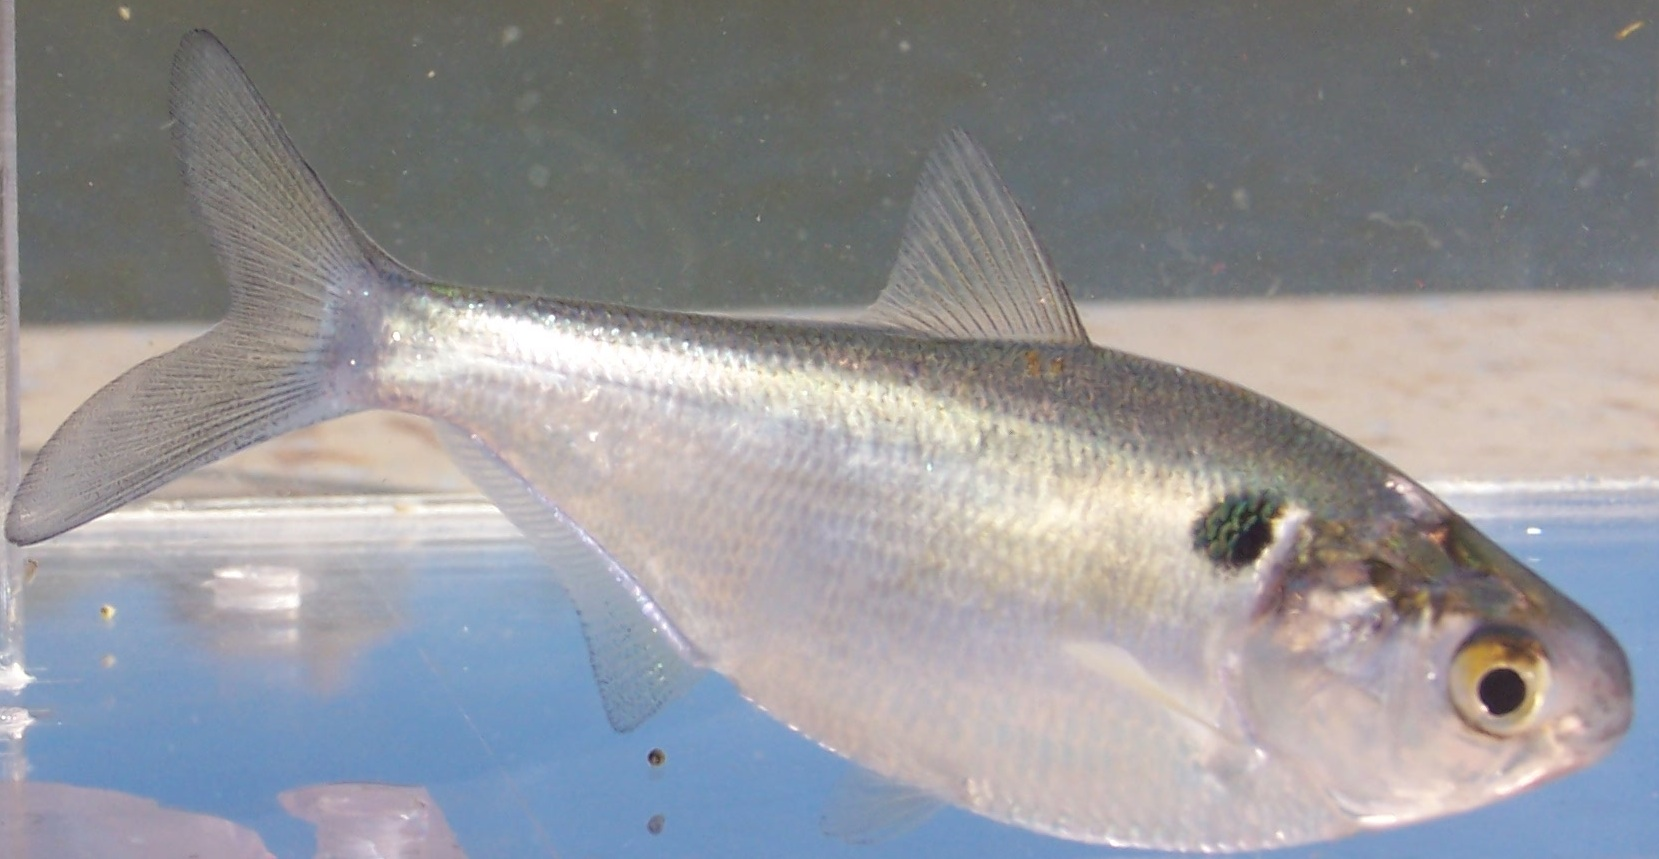
\includegraphics[keepaspectratio]{figs/gizzard_shad.jpg}}

}

\subcaption{\label{fig-shad}Gizzard shad}

\end{minipage}%
%
\begin{minipage}{0.46\linewidth}

\centering{

\pandocbounded{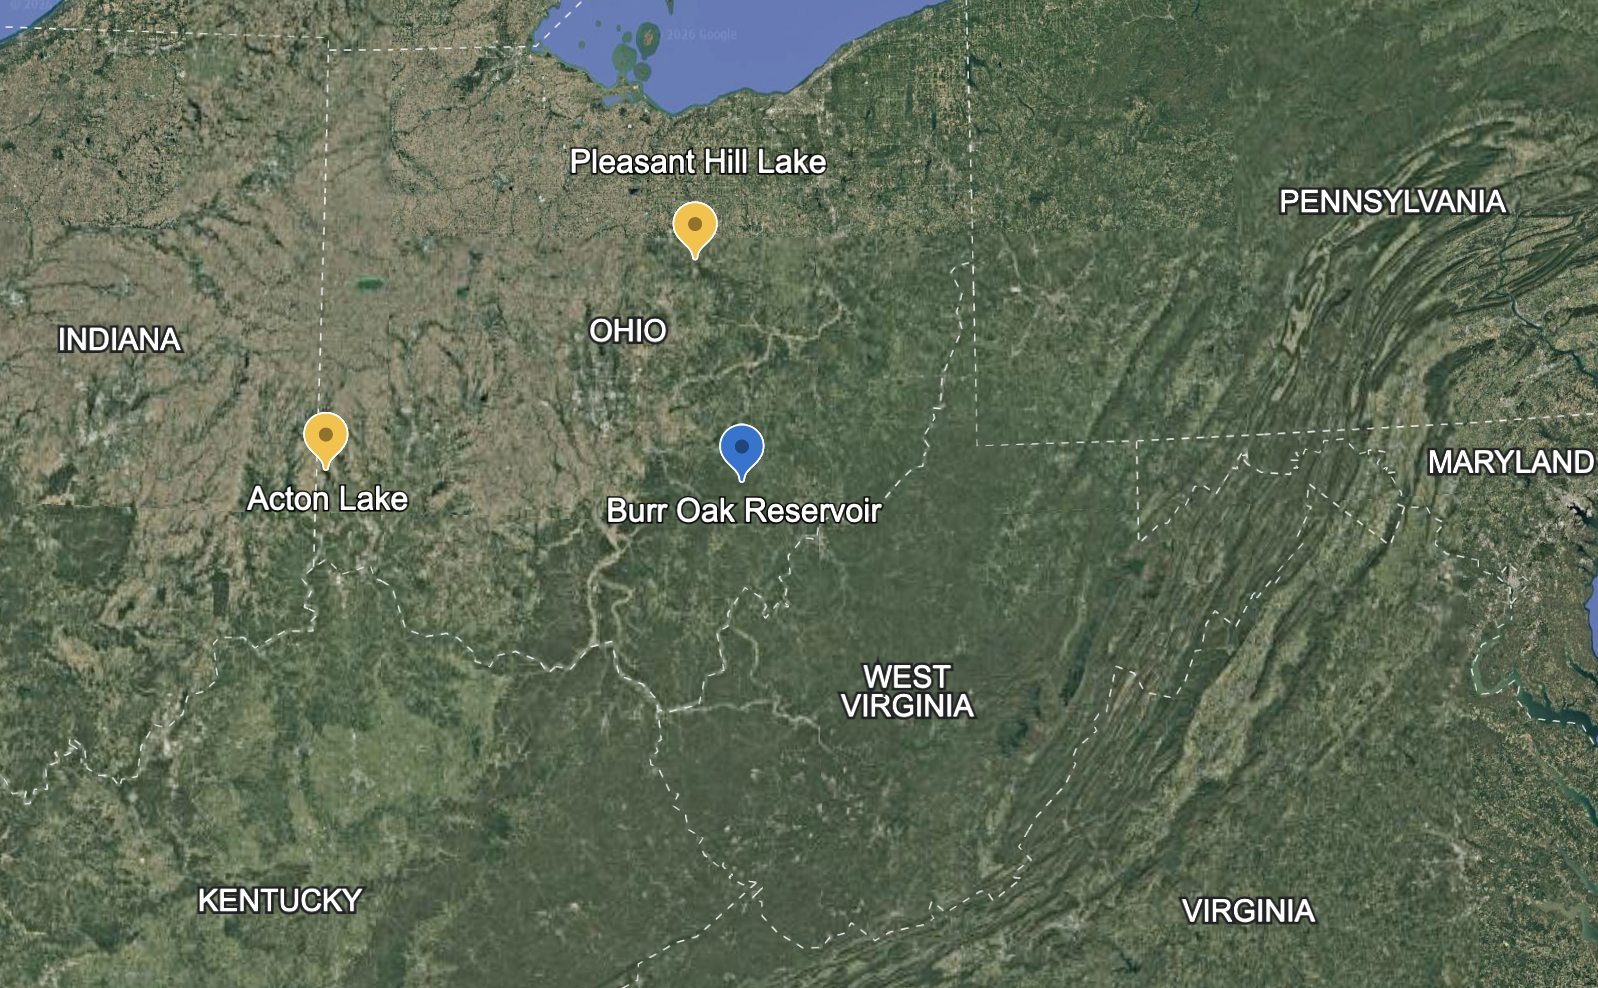
\includegraphics[keepaspectratio]{figs/reservoirs.png}}

}

\subcaption{\label{fig-res}Three reservoirs}

\end{minipage}%

\caption{\label{fig-shad}Gizzard shad, \emph{Dorosoma cepedianum}, are
probably the most abundant fish (by biomass) in lakes of the southern
and lower Midwest USA. They eat mud---sediment detritus from lake
bottoms---and in doing so they cycle enormous quantities of nitrogen and
phosphorus back into the water, fueling algal growth. In some lakes,
nutrient fluxes mediated by gizzard shad support more than 25\% of algal
primary production. The data we use in this chapter were collected from
gizzard shad at three man-made lakes (reservoirs) in Ohio, U.S.A.
(Schaus et al.~1997, Higgins et al.~2006). Shad photo courtesy M.J.
Vanni.}

\end{figure}%

\section{Acknowledgement}\label{acknowledgement}

This chapter is an R version of Vanni and Gephart (2011). I am grateful
to Mike and Jessica and the Ecological Society of America for making the
data and the article available.

\section{Goals}\label{goals-11}

In this chapter, you will explore how two fundamental properties of
organisms---body size and temperature---control rates of nutrient
cycling. Along the way, you will test specific quantitative predictions
of the \textbf{Metabolic Theory of Ecology} (MTE), and discover how well
those predictions hold up under real field conditions.

If you successfully complete this chapter, you will be able to

\begin{itemize}
\tightlist
\item
  explain how metabolic rates scale with body size (allometry),
\item
  explain how metabolic rates depend on temperature (\(Q_{10}\)),
\item
  use log-transformations to linearize power-law relationships,
\item
  fit and interpret linear regressions in R,
\item
  evaluate the support for specific quantitative hypotheses, and
\item
  reason about how body size and temperature act simultaneously on a
  biological rate.
\end{itemize}

\section{Preparatory steps}\label{preparatory-steps-8}

\begin{enumerate}
\def\labelenumi{\arabic{enumi}.}
\tightlist
\item
  General background: Read the sections below on allometry and
  temperature dependence. If your instructor has assigned background
  readings or lectures on metabolic ecology, complete those first.
\item
  Data: go to our
  \href{https://drive.google.com/drive/u/1/folders/1FR2FLiW3xyD4Er52YzVTToPZuXXReGRo}{class
  data repository}, and download \texttt{fish\_nutrient\_excretion.csv}.

  \begin{enumerate}
  \def\labelenumii{\alph{enumii}.}
  \tightlist
  \item
    Put \texttt{fish\_nutrient\_excretion.csv} in your \texttt{data}
    directory (inside \texttt{Rwork}).
  \end{enumerate}
\item
  Find out what you need for the deliverables
  (Section~\ref{sec-deliv-metabolic}).
\end{enumerate}

\section{Background}\label{background-9}

\subsection{The Metabolic Theory of Ecology: Why body size and
temperature
matter}\label{the-metabolic-theory-of-ecology-why-body-size-and-temperature-matter}

The metabolic rates of organisms---plants, microbes, and animals---are
strongly influenced by body size and body temperature (Gillooly et al.
2001; Brown et al. 2004). Large organisms obviously have higher
metabolic rates than small ones, when rates are expressed on a \emph{per
individual} basis. And because biochemical reactions are
temperature-dependent, most metabolic rates increase with body
temperature, at least up to some upper tolerance limit.

Understanding how biological rates scale with size and temperature is
important for several reasons. There is enormous variation in body size
among Earth's life forms, from tiny bacteria to great whales and giant
sequoia trees. Even within a single species, body size can vary
dramatically. Knowledge of how rates vary with size tells us how
individuals of different sizes use resources, process materials like
nutrients and energy, and interact with other species. Similarly,
because organisms experience a wide range of temperatures---both
naturally and increasingly due to human activity---understanding
temperature effects helps us predict how organisms and ecosystems may
respond to environmental change.

The \textbf{Metabolic Theory of Ecology} (MTE) provides mechanistic
explanations for these relationships (West, Brown, and Enquist 1997;
Brown et al. 2004; Banavar et al. 2014). The theory describes how
diffusion and diffusion networks in an individual organism cause body
size alone to exert a strong and predictable effect on whole-organism
metabolic rate. This theory also describes how the temperature
regulation of biochemical processes at the molecular level has a
similarly profound and predictable influence on whole-organism metabolic
rate. Notably, and in contrast to most ecological theory, MTE makes
predictions about the quantitative effects of body size and temperature
metabolic rate.

At the base of all the explanation is the geometry of the resource
distribution system (vascular system, simple 3D diffusion). All
organisms take in limiting resources and have to distribute those
resources to each part of each cell in the body. The key point is that
\emph{the larger the organism, the greater the portion of the resources
are in transit at any instant in time}. This leads to an increasingly
inefficient system, in which the metabolism of larger organisms has to
run more slowly per unit resource:

\subsection{Allometry: how rates scale with body
size}\label{allometry-how-rates-scale-with-body-size}

At a constant temperature, the effect of body size on metabolic rate can
be described with a simple power law:

\begin{equation}\phantomsection\label{eq-allometry}{B = B_0 M^z}\end{equation}

where \(B\) is the organism's metabolic rate (e.g., micromoles of
nitrogen excreted per hour), \(B_0\) is a normalization constant, \(z\)
is the \textbf{allometric scaling exponent}, and \(M\) is the organism's
body mass.

\begin{tcolorbox}[enhanced jigsaw, toprule=.15mm, colframe=quarto-callout-note-color-frame, bottomrule=.15mm, arc=.35mm, breakable, leftrule=.75mm, rightrule=.15mm, bottomtitle=1mm, coltitle=black, left=2mm, titlerule=0mm, title={Follow the Logic: Why log-transform?}, toptitle=1mm, colbacktitle=quarto-callout-note-color!10!white, opacityback=0, colback=white, opacitybacktitle=0.6]

Equation~\ref{eq-allometry} is a \emph{power law}---the dependent
variable (\(B\)) is a power function of the independent variable
(\(M\)). Power laws are curved on arithmetic axes, which makes them hard
to interpret visually and statistically. But watch what happens when we
take the logarithm of both sides:

\begin{equation}\phantomsection\label{eq-allometry-log}{\log B = \log B_0 + z \cdot \log M}\end{equation}

This is the equation of a straight line! The slope is \(z\) (the
allometric exponent) and the intercept is \(\log B_0\). This is why
ecologists plot metabolic data on log-log axes: it turns a curved
relationship into a linear one, and the slope tells us directly how
metabolic rate scales with body size.

This is a case where the mathematics \emph{is} the ecological reasoning.
The log-transformation isn't just a trick to make a pretty graph---it
reveals the fundamental scaling relationship and lets us estimate the
parameter (\(z\)) that captures how biology works.

\end{tcolorbox}

Allometric theory and extensive empirical data show that for many
biological rates, the increase in metabolic rate is less than
proportional to the increase in body mass. Mathematically, this means
\(b < 1\), sometimes called \textbf{negative allometry}. The
\textbf{Metabolic Theory of Ecology} (MTE) makes a very specific
prediction: \(b = 0.75\) (West, Brown, and Enquist 1997; Brown et al.
2004; Banavar et al. 2014). This prediction arises from theory about how
resource distribution networks (like circulatory systems) scale with
body size.

To get a feel for why \(b < 1\) matters, consider this: an elephant
(\(5 \times 10^6\) g) weighs about 500,000 times more than a mouse (10
g). If \(b = 0.75\), the elephant's metabolic rate is only about 19,000
times greater than the mouse's---proportionally much less than the
difference in body mass. Per gram, the mouse burns hotter.

Thus, Larger organisms can process more resources per unit time
(\(B=aM^{3/4}\)), but do so less and less efficiently
(\(\frac{B}{M}=aM^{-1/4}\)) due to resources in transport.

However, the prediction that \(b = 0.75\) is somewhat controversial.
Some data suggest that the exponent is closer to 1.0 for many organisms
(e.g., Reich et al. 2006), and others argue that \(b \approx 0.75\) only
when averaged across many species but varies considerably among them
(Isaac and Carbone 2010).

\subsection{Temperature dependence and the Arrhenius
Equation}\label{temperature-dependence-and-the-arrhenius-equation}

In addition to the role of body size, MTE incorporates the effects of
temperature. Gillooly et al. (2001) showed that metabolic rate can be
predicted from both body mass and body temperature:

\begin{equation}\phantomsection\label{eq-mte-full}{B = B_0 M^z e^{-E_a/(kT)}}\end{equation}

where \(e\) is the base of the natural logarithm, \(Ea\) is the
activation energy of metabolic enzymes, \(k\) is Boltzmann's constant
(\(8.617 \times 10^{-5}\) eV K\(^{-1}\)), and \(T\) is temperature in
Kelvin.\footnote{Recall Kelvin degrees = Celsius degrees + 273.15}

In the late 1800s, Svante Arrhenius described the power law relation for
the temperature dependence of chemical reaction rates; you may have
encountered this in your chemistry class. This was further quantified
and explained using first principles of entropy and probability by
Ludwig Boltzmann.\footnote{Boltzmann's work on this and on
  \emph{entropy} have connections throughout science, including Planck's
  constant and blackbody radiation, and even the meaning of time.}
Boltzmann showed how the emergent property of ``temperature'' emerges
from the thermal energy of individual particles. Later, Max Planck
further explicated this quantity, referring to the specific quantity as
\(k\), and then named it after Boltzmann. You will also encounter
Boltzmann's constant in our last chapter, on global heating.

\subsection{Nutrient excretion by
fish}\label{nutrient-excretion-by-fish}

Most experimental tests of MTE have been done in the lab, where
activity, temperature, and diet can be controlled and we can measure
\emph{basal metabolic rate} (i.e.~base metabolic rate, at rest). But
organisms in nature are often active, experience variable temperatures,
and are feeding---they display \emph{active metabolic rates.} Far fewer
studies have tested whether MTE predictions hold under field conditions,
where diet, activity, and other factors add noise.

Excretion rate is a type of whole-organism metabolic rate. It is an
output of many metabolic processes, and it represents the quantity of
nutrient released after maintenance and growth needs are met.

This output from the metabolic processes of many individuals has
important consequences (Sterner, Elser, and Vitousek 2002). This
excretion of nitrogen (N) and phosphorus (P) by fish is ecologically
important because these nutrients, released in dissolved form that algae
can readily use, can fuel a significant fraction of primary production
in lakes (Vanni et al. 2006).

\section{Using logarithms}\label{using-logarithms}

It is common to express these relationships on a logarithmic scale, and
we do this for two reasons. First, it expresses the relations on a
relative in which multiplicative differences are shown as additive and
our brains can understand additive differences more eaasily. Second,
using a logarithmic scale linearizes the relations and allows us to more
easily estimate the parameters of interest: \(z\) (allometric scaling)
and \(E_a\) (temperature sensitivity).

Taking the logarithms of Equation~\ref{eq-mte-full}, we have
\[\ln (B) = \ln (B_0) + z \ln (M) - E_a \frac{1}{kT}\]

where \(k\) is Boltzmann's constant and \(T\) is temperature in degrees
Kelvin. Below, we will start with the raw data and create new variables
of \(\ln (B)\), \(\ln (M)\), and \(1/(kT)\).

\section{Hypotheses, our data, and
predictions}\label{hypotheses-our-data-and-predictions}

Once we know what data we have available to us, we can use our
hypotheses to make specific predictions about those data. Remember that
a \emph{scientific hypothesis} should be a general explanation of a
process or pattern in nature, anbd \emph{prediction} is a logical
deduction that follows when we apply that general explanation to a
particular system.\footnote{Recall that a \emph{scientific theory} is a
  very strongly supported and even more general set of explanations that
  provides framework to organize our well-supported ideas and helps us
  generate new hypotheses.}

So, logic follows in this manner:

The MTE describes the ecological consequences of body size and
temperature. Given that theory, we can hypothesize that 1. because the
metabolic rate of larger bodied organisms scale to the 3/4 power of
size, fish nutrient excretion rate should also scale in the same manner;
and 1. because the metabolic rate of warmer organisms scale with
temperature by a factor of \(E_a/(kT)\) where \(E_a \approx 0.23\), fish
nutrient excretion rate should also scale in the same manner.

What data do we have?

The data we will analyze come from field studies of nutrient excretion
by gizzard shad (\emph{Dorosoma cepedianum}) in three Ohio lakes
\href{@fig-res}{Schaus et al. (1997); Higgins, Vanni, and González
(2006)}. We have excretion data for 200 individual fish. These 200 fish
are a tiny fraction of the fish in these lakes, but they represent a
useful sample from which we can extrapolate.

Individual fish were captured, placed in filtered lake water, and
investigators measured the change in (i) dissolved N and (ii) P
concentration over a fixed period of time. The variables in the data set
are:

\begin{itemize}
\tightlist
\item
  \texttt{temp\_C} --- water temperature (°C) experienced by the fish
\item
  \texttt{mass\_g} --- wet body mass (grams)
\item
  \texttt{N\_u.h} --- nitrogen excretion rate (\(\mu\)mol N per fish per
  hour)
\item
  \texttt{P\_u.h} --- phosphorus excretion rate (\(\mu\)mol P per fish
  per hour)
\end{itemize}

\subsection{Predictions}\label{predictions-2}

\textbf{Given our hypotheses and the data we have, we \emph{predict}
that gizzard shad nutrient excretion rate will scale with the 3/4 power
of gizzard shad body mass, and by a factor of by a factor of \(E_a\)
with the inverse of temperature \(1/T\).}

\textbf{You will use multiple linear regression to evaluate those
predictions.}

\section{Getting R ready for work}\label{getting-r-ready-for-work}

Open R using RStudio, and load the packages we'll need. Note that we
will use a new package, \texttt{broom}. You will need to install
\texttt{broom} if you hadn't done so for some other exercise or your own
research.

To install \texttt{broom}, you can use the \emph{Tools} drop-down menu
in RStudio, or run this code:

\begin{Shaded}
\begin{Highlighting}[]
\FunctionTok{install.packages}\NormalTok{(}\StringTok{"broom"}\NormalTok{)}
\end{Highlighting}
\end{Shaded}

Now load \texttt{broom}, and \texttt{tidyverse} if you have not already
done so.

\begin{Shaded}
\begin{Highlighting}[]
\FunctionTok{library}\NormalTok{(tidyverse)}
\FunctionTok{library}\NormalTok{(broom)}
\end{Highlighting}
\end{Shaded}

Now read in the data and take a look.

\begin{Shaded}
\begin{Highlighting}[]
\CommentTok{\# Note we skip the first 8 lines because they are \textquotesingle{}metadata\textquotesingle{},}
\CommentTok{\# which is \textquotesingle{}data about data\textasciigrave{} or information about the variables.}

\NormalTok{fish }\OtherTok{\textless{}{-}} \FunctionTok{read.csv}\NormalTok{(}\StringTok{"data/fish\_nutrient\_excretion.csv"}\NormalTok{, }\AttributeTok{skip=}\DecValTok{8}\NormalTok{)}
\FunctionTok{glimpse}\NormalTok{(fish)}
\end{Highlighting}
\end{Shaded}

\begin{verbatim}
Rows: 200
Columns: 5
$ Fish_ID <int> 1, 2, 3, 4, 5, 6, 7, 8, 9, 10, 11, 12, 13, 14, 15, 16, 17, 18,~
$ temp_C  <dbl> 16.4, 16.4, 16.4, 16.4, 16.4, 16.4, 16.4, 16.4, 16.4, 16.4, 16~
$ mass_g  <dbl> 4.50, 5.40, 5.75, 5.80, 5.95, 9.20, 10.90, 11.10, 11.65, 11.80~
$ N_u.h   <dbl> 2.45, 10.67, 14.89, 21.69, 20.14, 25.25, 31.93, 9.40, 37.01, 3~
$ P_u.h   <dbl> 1.71, 2.16, 1.66, 1.49, 2.14, 3.21, 1.99, 2.69, 2.48, 3.91, 2.~
\end{verbatim}

\begin{Shaded}
\begin{Highlighting}[]
\FunctionTok{summary}\NormalTok{(fish)}
\end{Highlighting}
\end{Shaded}

\begin{verbatim}
    Fish_ID           temp_C          mass_g           N_u.h       
 Min.   :  1.00   Min.   :16.40   Min.   :  2.32   Min.   :  2.45  
 1st Qu.: 50.75   1st Qu.:18.50   1st Qu.: 21.93   1st Qu.: 62.88  
 Median :100.50   Median :23.10   Median : 46.00   Median :119.34  
 Mean   :100.50   Mean   :22.54   Mean   : 49.16   Mean   :150.75  
 3rd Qu.:150.25   3rd Qu.:25.50   3rd Qu.: 65.28   3rd Qu.:213.14  
 Max.   :200.00   Max.   :29.40   Max.   :210.94   Max.   :524.29  
     P_u.h       
 Min.   : 0.590  
 1st Qu.: 4.975  
 Median : 9.950  
 Mean   :12.304  
 3rd Qu.:17.273  
 Max.   :50.660  
\end{verbatim}

You should have 200 rows and 5 columns. The fish range in mass from
about 2 g to over 200 g, and temperatures range from about 16°C to 29°C.

What are 16°C to 29°C in Fahrenheit degrees? (The conversion factor is
\(Y^\circ\, \mathrm(F) =  \frac{180}{100} X^\circ\, \mathrm{C} + 32\))

\section{Exploring the data}\label{exploring-the-data}

We already know that we will want to create a few new variables based on
the raw data, including the logs of excretion rates, mass and the
inverse of temperature in Kelvin. Below we do that.

First, here is the value of Boltzmann's constant, in units of electron
volts per degree Kelvin

\begin{Shaded}
\begin{Highlighting}[]
\NormalTok{boltzmann\_k }\OtherTok{\textless{}{-}} \FloatTok{8.617333262e{-}5}
\end{Highlighting}
\end{Shaded}

Now we transform our variables.

\begin{Shaded}
\begin{Highlighting}[]
\DocumentationTok{\#\# Add log{-}transformed columns to the data}
\NormalTok{fish }\OtherTok{\textless{}{-}}\NormalTok{ fish }\SpecialCharTok{\%\textgreater{}\%} \CommentTok{\#start with our fish data set, and}
  \FunctionTok{mutate}\NormalTok{(}\AttributeTok{log\_mass =} \FunctionTok{log}\NormalTok{(mass\_g), }\CommentTok{\# create ln(mass)}
         \AttributeTok{log\_N =} \FunctionTok{log}\NormalTok{(N\_u.h), }\CommentTok{\# ln(N excretion)}
         \AttributeTok{log\_P =} \FunctionTok{log}\NormalTok{(P\_u.h), }\CommentTok{\# ln(P excretion)}
         \AttributeTok{temp\_K =} \FloatTok{273.15} \SpecialCharTok{+}\NormalTok{ temp\_C, }\CommentTok{\# degrees Kelvin}
         \AttributeTok{inv.kT =} \DecValTok{1}\SpecialCharTok{/}\NormalTok{(boltzmann\_k }\SpecialCharTok{*}\NormalTok{ temp\_K) }\CommentTok{\# inverse scaled Kelvin}
\NormalTok{  )}
\end{Highlighting}
\end{Shaded}

Before testing any hypotheses, let's look at the data. Always plot your
data before you analyze it.

\subsection{Raw-scale plots}\label{raw-scale-plots}

\begin{Shaded}
\begin{Highlighting}[]
\FunctionTok{ggplot}\NormalTok{(fish, }\FunctionTok{aes}\NormalTok{(}\AttributeTok{x =}\NormalTok{ mass\_g, }\AttributeTok{y =}\NormalTok{ N\_u.h)) }\SpecialCharTok{+}
  \FunctionTok{geom\_point}\NormalTok{(}\AttributeTok{alpha =} \FloatTok{0.5}\NormalTok{) }\SpecialCharTok{+}
  \FunctionTok{labs}\NormalTok{(}\AttributeTok{x =} \StringTok{"Body mass (g)"}\NormalTok{,}
       \AttributeTok{y =} \FunctionTok{expression}\NormalTok{(}\FunctionTok{paste}\NormalTok{(}\StringTok{"N excretion ("}\NormalTok{, mu, }\StringTok{"mol "}\NormalTok{, fish}\SpecialCharTok{\^{}}\NormalTok{\{}\SpecialCharTok{{-}}\DecValTok{1}\NormalTok{\}, }\StringTok{" "}\NormalTok{, hr}\SpecialCharTok{\^{}}\NormalTok{\{}\SpecialCharTok{{-}}\DecValTok{1}\NormalTok{\}, }\StringTok{")"}\NormalTok{)),}
       \AttributeTok{title =} \StringTok{"N excretion vs. body mass"}\NormalTok{) }\SpecialCharTok{+}
  \FunctionTok{theme\_minimal}\NormalTok{()}
\end{Highlighting}
\end{Shaded}

\begin{figure}[H]

\centering{

\pandocbounded{
\includegraphics[keepaspectratio]{14-metabolic-ecology_v_2_files/figure-pdf/fig-raw-N-1.pdf}}

}

\caption{\label{fig-raw-N}Nitrogen excretion rate vs.~body mass on
arithmetic (raw) axes.}

\end{figure}%

Make a similar plot for P excretion rate. What do you notice about the
shape of these relationships? They are curved---larger fish excrete
more, but the relationship is not a straight line.

\subsection{Log-transformed plots}\label{log-transformed-plots}

Now let's see what happens when we log-transform both axes, as suggested
by the allometric equation (Equation~\ref{eq-allometry-log}).

\begin{Shaded}
\begin{Highlighting}[]
\FunctionTok{ggplot}\NormalTok{(fish, }\FunctionTok{aes}\NormalTok{(}\AttributeTok{x =} \FunctionTok{log}\NormalTok{(mass\_g), }\AttributeTok{y =} \FunctionTok{log}\NormalTok{(N\_u.h))) }\SpecialCharTok{+}
  \FunctionTok{geom\_point}\NormalTok{(}\AttributeTok{alpha =} \FloatTok{0.5}\NormalTok{) }\SpecialCharTok{+}
  \FunctionTok{labs}\NormalTok{(}\AttributeTok{x =} \FunctionTok{expression}\NormalTok{(log[}\DecValTok{10}\NormalTok{]}\SpecialCharTok{\textasciitilde{}}\StringTok{"(body mass, g)"}\NormalTok{),}
       \AttributeTok{y =} \FunctionTok{expression}\NormalTok{(log[}\DecValTok{10}\NormalTok{]}\SpecialCharTok{\textasciitilde{}}\StringTok{"(N excretion, "} \SpecialCharTok{*}\NormalTok{ mu }\SpecialCharTok{*} \StringTok{"mol "} \SpecialCharTok{*}\NormalTok{ fish}\SpecialCharTok{\^{}}\NormalTok{\{}\SpecialCharTok{{-}}\DecValTok{1}\NormalTok{\} }\SpecialCharTok{*} \StringTok{" "} \SpecialCharTok{*}\NormalTok{ hr}\SpecialCharTok{\^{}}\NormalTok{\{}\SpecialCharTok{{-}}\DecValTok{1}\NormalTok{\} }\SpecialCharTok{*} \StringTok{")"}\NormalTok{),}
       \AttributeTok{title =} \StringTok{"Allometric scaling of N excretion"}\NormalTok{) }\SpecialCharTok{+}
  \FunctionTok{theme\_minimal}\NormalTok{()}
\end{Highlighting}
\end{Shaded}

\begin{figure}[H]

\centering{

\pandocbounded{
\includegraphics[keepaspectratio]{14-metabolic-ecology_v_2_files/figure-pdf/fig-log-N-1.pdf}}

}

\caption{\label{fig-log-N}Log nitrogen excretion rate vs.~log body mass.
If the allometric model holds, this should be approximately linear.}

\end{figure}%

That looks much more linear! The log-transformation did exactly what
Equation~\ref{eq-allometry-log} predicted. Make the same plot for P
excretion.

MTE also suggests that temperature might influence excretion rates. Here
we plot separate rate vs.~mass graphs for each temperature:

\begin{Shaded}
\begin{Highlighting}[]
\FunctionTok{ggplot}\NormalTok{(fish, }\FunctionTok{aes}\NormalTok{(}\AttributeTok{x =}\NormalTok{ log\_mass, }\AttributeTok{y =}\NormalTok{ log\_N)) }\SpecialCharTok{+}
  \FunctionTok{geom\_point}\NormalTok{(}\AttributeTok{alpha =} \FloatTok{0.5}\NormalTok{) }\SpecialCharTok{+}
  \FunctionTok{geom\_smooth}\NormalTok{(}\AttributeTok{method =} \StringTok{"lm"}\NormalTok{, }\AttributeTok{se =} \ConstantTok{TRUE}\NormalTok{) }\SpecialCharTok{+}
  \FunctionTok{facet\_wrap}\NormalTok{(}\SpecialCharTok{\textasciitilde{}}\NormalTok{temp\_C) }\SpecialCharTok{+} 
  \FunctionTok{labs}\NormalTok{(}\AttributeTok{x =} \FunctionTok{expression}\NormalTok{(log}\SpecialCharTok{\textasciitilde{}}\StringTok{"(body mass, g)"}\NormalTok{),}
       \AttributeTok{y =} \FunctionTok{expression}\NormalTok{(log}\SpecialCharTok{\textasciitilde{}}\StringTok{"(N excretion)"}\NormalTok{),}
       \AttributeTok{title =} \StringTok{"Allometric scaling of N excretion"}\NormalTok{) }\SpecialCharTok{+}
  \FunctionTok{theme\_minimal}\NormalTok{()}
\end{Highlighting}
\end{Shaded}

\begin{verbatim}
`geom_smooth()` using formula = 'y ~ x'
\end{verbatim}

\begin{figure}[H]

\centering{

\pandocbounded{
\includegraphics[keepaspectratio]{14-metabolic-ecology_v_2_files/figure-pdf/fig-regression-N1-1.pdf}}

}

\caption{\label{fig-regression-N1}Linear regression of log N excretion
on log body mass, for each temperature.}

\end{figure}%

\subsection{Allometric and temperature scaling of excretion
rates}\label{sec-assign1}

Here you need to estimate the allometric scaling exponent (\(z\)) and
the energy of activation (aka temperature sensitivity) for both N and P
excretion rates. Multiple regression will let us address a key question
how we can how do you deal with the fact that excretion rates were
measured at different temperatures?

There is more than one reasonable approach. Think about this before
reading on. One approach is to pool all the data together and fit a
single multiple regression. Another is to fit separate regressions for
each temperature and then compare slopes. You could try both and think
about what you learn from each approach.

\subsubsection{Mulltiple linear
regression}\label{mulltiple-linear-regression}

Now fit a linear regression for log N excretion vs.~log mass and inverse
temperature.

\begin{Shaded}
\begin{Highlighting}[]
\DocumentationTok{\#\# Fit the regression}
\NormalTok{m\_N\_all }\OtherTok{\textless{}{-}} \FunctionTok{lm}\NormalTok{(log\_N }\SpecialCharTok{\textasciitilde{}}\NormalTok{ log\_mass }\SpecialCharTok{+}\NormalTok{ inv.kT, }\AttributeTok{data =}\NormalTok{ fish)}
\end{Highlighting}
\end{Shaded}

If it ran without error, you are ready for the next step.

\textbf{Next step: check your assumptions}

All statistical models have builit-in assumptions. The regression we ran
here assumes, among other things, that the relationships are linear and
the unexplained noise in the data are normally distributed, both above
and below the expected or fitted values. Here we examin that
graphically.

\begin{Shaded}
\begin{Highlighting}[]
\FunctionTok{plot}\NormalTok{(m\_N\_all, }\AttributeTok{which=}\DecValTok{1}\NormalTok{)}
\end{Highlighting}
\end{Shaded}

\pandocbounded{
\includegraphics[keepaspectratio]{14-metabolic-ecology_v_2_files/figure-pdf/unnamed-chunk-8-1.pdf}}

If these assumptions are met, then the \emph{residual} unexplained noise
is just as likely to be positive and negative for any fitted value. And
that is essentially what we see. Thus these assumptions appear to be
met.

\subsubsection{Evaluating the
predictions}\label{evaluating-the-predictions}

Recall that our equation is now

\[\ln (B) = \ln (B_0) + z \ln (M) - E_a \frac{1}{kT}\] and our
regression will estimate \(z\) for log mass, and \(E_a\) for inverse
scaled temperature. Here are the 95\% \emph{confidence intervals} on
those.

A \emph{confidence interval} (CI) is essentially a \emph{procedure},
rather than a thing. A 95\% CI is a procedure wherein if you repeated
the experiment many, many times, the CIs would capture the true estimate
about 95\% of the time.

Here are the confidence intervals for \(z\) (for log mass) and \(E_a\)
(for inverse scaled temperature).

\begin{Shaded}
\begin{Highlighting}[]
\DocumentationTok{\#\# View the results}
\CommentTok{\# ignore the intercept}
\FunctionTok{confint}\NormalTok{(m\_N\_all)}
\end{Highlighting}
\end{Shaded}

\begin{verbatim}
                 2.5 %     97.5 %
(Intercept) 11.4522604 21.4184325
log_mass     0.7062991  0.8718949
inv.kT      -0.4957793 -0.2478470
\end{verbatim}

\subsubsection{\texorpdfstring{\textbf{Do the same} for P
excretion.}{Do the same for P excretion.}}\label{do-the-same-for-p-excretion.}

\subsection{Thinking bigger: ecosystem
consequences}\label{thinking-bigger-ecosystem-consequences}

We have focused on excretion by individual fish. But remember the bigger
picture (Figure~\ref{fig-shad}): gizzard shad are extremely abundant in
many Midwestern lakes. They consume sediment detritus, extract what they
need, and excrete the rest as dissolved N and P that algae can
immediately use.

Consider this: if you know the allometric scaling exponent and \(E_a\),
and you know the size distribution and temperature regime of a lake, you
could \emph{predict} the total nutrient flux from the fish population to
the water column. This is exactly the kind of scaling-up that makes
metabolic ecology so powerful---and so important for understanding
ecosystem function.

\section{Deliverables}\label{sec-deliv-metabolic}

Compile the following into one document and submit by the due date. Turn
in a Word document or PDF with the following:

\begin{enumerate}
\def\labelenumi{\arabic{enumi}.}
\tightlist
\item
  Log-log scatter plots of N and P excretion vs.~body mass for each
  temperature.
\item
  Confidence intervals of the allometric scaling exponent (\(z\)) for
  both N and P excretion, and for temperature sensitivity (\(E_a\)).
\item
  Address these questions:

  \begin{enumerate}
  \def\labelenumii{\alph{enumii}.}
  \tightlist
  \item
    How well do the predictions of the Metabolic Theory of Ecology hold
    up for nutrient excretion by fish under field conditions? What
    specific factor or factors might cause deviations from MTE
    predictions in the field?
  \item
    Suppose a lake warms by 2°C due to climate change. Based on your
    \(E_a\) estimate, by how much would individual excretion rates
    change?
  \item
    If warming also shifts the fish population toward smaller body sizes
    (as has been observed in some systems), how would that interact with
    the temperature effect on total nutrient flux?
  \end{enumerate}
\end{enumerate}

\bookmarksetup{startatroot}

\chapter{An Introduction to the Carbon Cycle and Global
Heating}\label{an-introduction-to-the-carbon-cycle-and-global-heating}

\begin{figure}

\centering{


\includegraphics[width=0.75\linewidth,height=\textheight,keepaspectratio]{figs/ecosystems1.png}

}

\caption{\label{fig-ecosys1}Ecosystems comprise pools (compartments) and
fluxes in and out of those pools. Ecosystem ecologists typically study
ecosystems by tracking a particular chemical element from compartment to
compartment. Note the units are consistent throughout an ecosystem. In
the above example of a lake, fluxes of phosphorus are milligrams per day
in or out. At the global scale, we can estimate fluxes of carbon in
gigatonnes per year.}

\end{figure}%

\section{Goals}\label{goals-12}

In this chapter, you will provide partial answers for these questions:

\begin{enumerate}
\def\labelenumi{\arabic{enumi}.}
\tightlist
\item
  Why do we have this much carbon in the atmosphere?
\item
  How does including the physical process of diffusion of alter
  predictions about future atmospheric carbon?
\item
  What is the connection between atmospheric CO\(_2\) and temperature,
  and how does that relationship affect our appreciation of Earth's
  current and future status?
\end{enumerate}

To address these questions, we will use pencil and paper and R to,

\begin{enumerate}
\def\labelenumi{\arabic{enumi}.}
\tightlist
\item
  build a simple ecosystem budget with steady fluxes and changing pools,
\item
  create a dynamic ecosystem in which the fluxes change, depending on
  the amount in pools, and
\item
  investigate how matter can relate dynamically to energy.
\end{enumerate}

One of the main the points of doing these activities is to help to
develop an intuition for \emph{systems thinking}. A system is
``\href{https://en.wikipedia.org/wiki/Systems_theory}{a group of
interacting, interdependent parts that form a complex whole''} and
ecosystem ecology is a central subdisicpline of ecology and the one that
has contributed the most to our understanding of climate change and
ecosystem services.

The other main point of these activities is to reinforce simple ideas
related to the global carbon cycle and global warming.

\section{Preparatory steps}\label{preparatory-steps-9}

\begin{enumerate}
\def\labelenumi{\arabic{enumi}.}
\tightlist
\item
  General background lectures:
  \href{https://drive.google.com/drive/folders/1nWLoEGuWKIWdul9Uvse5qiB1Hf8MCwUv?usp=sharing}{Download
  and watch the video on the carbon cycle} before proceeding.
\item
  We will not need data for this chapter.
\item
  This chapter will ask you to complete some work by hand (without R)
  and turn that in in class. Find out what you need for the deliverables
  parts 1 (Section~\ref{sec-deliverables-ei1}) and 2
  (Section~\ref{sec-deliverables-ei2}).
\item
  Get some paper and pencil.
\item
  Get R ready for work - see the next section.
\end{enumerate}

\section{Get R ready for work}\label{get-r-ready-for-work}

Open R using RStudio, and \textbf{set your working directory}. You can
do this in two ways:

\begin{enumerate}
\def\labelenumi{\arabic{enumi}.}
\tightlist
\item
  using the Session menu in RStudio, or
\item
  with code such as this, in which you must customize it to your
  computer!
\end{enumerate}

\begin{verbatim}
setwd("C:/Users/chenjoe/BIO209W/Rwork")
\end{verbatim}

You can confirm or \textbf{get} your \emph{current} working directory
using this:

\begin{Shaded}
\begin{Highlighting}[]
\FunctionTok{getwd}\NormalTok{()}
\end{Highlighting}
\end{Shaded}

\begin{verbatim}
[1] "/Users/stevenmh/projects/intro_to_ecology"
\end{verbatim}

so when I do that, you can see my working directory is the one for this
book.

\textbf{Before you proceed}, make sure your working directory is your
\texttt{Rwork} directory.

Next, use RStudio to create a new file of the type \emph{R script}. Save
it using a name that reflects this chapter, and end the file name with
``.R'' or ``.r''.

Third, add a comment as a brief description of the script, and load any
R packages you know you will need.

\begin{Shaded}
\begin{Highlighting}[]
\DocumentationTok{\#\# This script is for chapter XX in Hank\textquotesingle{}s Intro to Ecology primer.}

\DocumentationTok{\#\# We always use...}
\FunctionTok{library}\NormalTok{(tidyverse)}
\DocumentationTok{\#\# or usually just ggplot2 and dplyr packages within the tidyverse.}
\DocumentationTok{\#\# In this chapter we also need}
\FunctionTok{library}\NormalTok{(deSolve)}
\CommentTok{\# for solving or integrating differential equations}
\end{Highlighting}
\end{Shaded}

\section{Background on ecosystems}\label{background-on-ecosystems}

An ecosystem is a biological community of interacting organisms and
their physical environment. Ecosystem ecologists study an ecosystem by
tracking a particular chemical element such as carbon (C) or nitrogen
(N) through the environment. We conceive of the environment in terms of
compartments that contain the element (a.k.a. pools, stocks) and
movement between compartments (fluxes, inflows, outflows).

Examples of ecosystem budgets:

\begin{itemize}
\tightlist
\item
  \textbf{Phosphorus budget of a lake ecosystem.} Phosphorus (P) flows
  in via a stream coming into the lake, and discharges in a stream
  leaving the lake.
\item
  \textbf{Carbon budget of Earth's atmosphere.}: Carbon enters as
  CO\(_2\) via biological respiration and fossil fuel combustion and
  exits via uptake in photosynthesis in land plants and aquatic algae,
  and also via diffusion into oceans.
\item
  \textbf{Energy budget of mountain stream.} Energy is captured from
  sunlight via photosynthesis in aquatic algae and falls in as dead
  leaves, and exits via molecules of CO\(_2\) respired by organisms and
  as organic molecules and particles flowing flowing downstream.
\end{itemize}

The ecosystem paradigm connects energy and matter to the evolution and
ecology of life. Ecosystem scientists focus on the flow of energy or
matter through all parts of the environment, especially as those flows
are mediated by living organisms.

\section{A simple budget provides one explanation for why we have so
much carbon in the
atmosphere}\label{a-simple-budget-provides-one-explanation-for-why-we-have-so-much-carbon-in-the-atmosphere}

Why do we have so much carbon in the atmosphere? One answer to that
question comes from simply tallying up the inputs and the outflows. In
this sense, it is a lot like our household budget.

Ecosystem budgets are simple\footnote{A \emph{zeroth order} flux is one
  in which the rate depends on the amounts in zero pools - it doesn't
  depend on pools.}, at least conceptually. An ecosystem budget is just
like your household budget or bank account: if more money goes in than
goes out, you accumulate money. In contrast, if you spend more money
than you bring in, your wealth declines.

An ecosystem budget simply keeps track of the amount of a chemical
element, such as nitrogen or carbon, that, is in a compartment, goes
into a compartment, and leaves a compartment, over a specified time
interval such as a year. The \textbf{size} of a pool or compartment is
the amount of an element in that pool.

\subsection{Rate of change}\label{rate-of-change}

For a simple ecosystem carbon budget, the \emph{rate of change} of the
size of a pool is the \textbf{difference} between the input and the
output over a specified time interval,

\[\Delta~\mathrm{Pool} = \mathrm{Inputs} - \mathrm{Outputs}\]

For instance, consider the carbon budget for Earth's atmosphere from the
1990's that we described in lecture. We had these inputs and outputs
(units are petagrams, 10\(^{15}\) g):

\begin{itemize}
\tightlist
\item
  Inputs to the atmosphere

  \begin{itemize}
  \tightlist
  \item
    diffusion from the ocean (respiration, 91 Pg/y)
  \item
    River outgassing (1 Pg/y)
  \item
    Fire (4 Pg/y)
  \item
    Cement production (0.1 Pg/y)
  \item
    Fossil fuel (7.6 Pg/y)
  \item
    Land use change (1.5 Pg/y)
  \item
    Terrestrial respiration (mostly soil microbes 56 Pg/y)
  \end{itemize}
\end{itemize}

These total to \(91+1+4+0.1+7.6+1.5+56=161\) Pg C / y.

\begin{itemize}
\tightlist
\item
  Outputs from the atmosphere

  \begin{itemize}
  \tightlist
  \item
    diffusion into the ocean (photosynthesis, and carbonic acid
    formation 92 Pg/y)
  \item
    Weathering (0.2 Pg/y)
  \item
    Land sink (2.8 Pg/y)
  \item
    NPP on land (60 Pg/y)
  \end{itemize}
\end{itemize}

These total to \(0.2 +2.8+60=161\) Pg C / y.

At the time, the \textbf{atmosphere held 762 Pg C} mostly in the forms
of carbon dioxide, carbon monoxide, and methane (CO\(_2\), CO,
CH\(_4\)).

Given this budget, how much carbon would be in the atmosphere,

\begin{itemize}
\tightlist
\item
  one year later?
\item
  two years later?
\item
  fifty years later?
\end{itemize}

To figure this out with a simple budget, we simply start with the pool,
add the inputs and subtract the outputs.
\[\mathrm{Atmosphere_{t+1}} = \mathrm{Atmosphere_{t}} + \mathrm{inputs} -  \mathrm{outputs}\]

Here we have inputs into the atmosphere.

\begin{Shaded}
\begin{Highlighting}[]
\NormalTok{or }\OtherTok{\textless{}{-}} \DecValTok{91} \CommentTok{\# diffusion out of the ocean, due to respiration of microbes}
\NormalTok{ro }\OtherTok{\textless{}{-}} \DecValTok{1} \CommentTok{\# river outgassing (diffusion)}
\NormalTok{fi }\OtherTok{\textless{}{-}} \DecValTok{4} \CommentTok{\# fire}
\NormalTok{cp }\OtherTok{\textless{}{-}} \FloatTok{0.1} \CommentTok{\# cement production}
\NormalTok{ff }\OtherTok{\textless{}{-}} \FloatTok{7.6} \CommentTok{\# fossil fuel combustion (1998) }
\NormalTok{lu }\OtherTok{\textless{}{-}} \FloatTok{1.5} \CommentTok{\# land use change }
\NormalTok{tr }\OtherTok{\textless{}{-}} \DecValTok{56} \CommentTok{\# terrestrial respiration}
\NormalTok{inputs }\OtherTok{\textless{}{-}}\NormalTok{ or }\SpecialCharTok{+}\NormalTok{ ro }\SpecialCharTok{+}\NormalTok{ fi }\SpecialCharTok{+}\NormalTok{ cp }\SpecialCharTok{+}\NormalTok{ ff }\SpecialCharTok{+}\NormalTok{ lu }\SpecialCharTok{+}\NormalTok{ tr}
\NormalTok{inputs}
\end{Highlighting}
\end{Shaded}

\begin{verbatim}
[1] 161.2
\end{verbatim}

Here we have outputs from the atmosphere mostly into plants on land and
into the oceans where most of it is taken up by phytoplankton, kelp,
seagrasses, and corals. A small amount of it remains in the water and
makes it more acidic.

\begin{Shaded}
\begin{Highlighting}[]
\NormalTok{npp.o }\OtherTok{\textless{}{-}} \DecValTok{92} \CommentTok{\# net primary production in the ocean (diffusion)}
\NormalTok{we }\OtherTok{\textless{}{-}} \FloatTok{0.2} \CommentTok{\# Weathering of carbonate rock}
\NormalTok{ls }\OtherTok{\textless{}{-}} \FloatTok{2.8} \CommentTok{\# land sink (burial)}
\NormalTok{npp.l }\OtherTok{\textless{}{-}} \DecValTok{60} \CommentTok{\# net primary production on land}

\NormalTok{outputs }\OtherTok{\textless{}{-}}\NormalTok{ npp.o }\SpecialCharTok{+}\NormalTok{ we }\SpecialCharTok{+}\NormalTok{ ls }\SpecialCharTok{+}\NormalTok{ npp.l}
\NormalTok{outputs}
\end{Highlighting}
\end{Shaded}

\begin{verbatim}
[1] 155
\end{verbatim}

The difference between inputs and outputs is \emph{net flux}:

\begin{Shaded}
\begin{Highlighting}[]
\NormalTok{net.flux }\OtherTok{\textless{}{-}}\NormalTok{ inputs }\SpecialCharTok{{-}}\NormalTok{ outputs}
\NormalTok{net.flux }\CommentTok{\# in Pg C per year}
\end{Highlighting}
\end{Shaded}

\begin{verbatim}
[1] 6.2
\end{verbatim}

At that time, Earth had a pool of carbon in the atmosphere of about 762
Pg C.

\begin{Shaded}
\begin{Highlighting}[]
\CommentTok{\# the pool}
\NormalTok{At }\OtherTok{\textless{}{-}} \DecValTok{762}
\end{Highlighting}
\end{Shaded}

So, what would it have one year later? It would have the pool plus the
net flux.

\begin{Shaded}
\begin{Highlighting}[]
\NormalTok{At.plus}\FloatTok{.1} \OtherTok{\textless{}{-}}\NormalTok{ At }\SpecialCharTok{+}\NormalTok{ net.flux}
\NormalTok{At.plus}\FloatTok{.1}
\end{Highlighting}
\end{Shaded}

\begin{verbatim}
[1] 768.2
\end{verbatim}

What about two years later? What about 3 or 25 or 75 years later? If we
choose to assume that these rates won't change, the answer is easy, but
only because we are working with a simple budget. We simply add the
annual flux for each year, starting at year 0.

\[\mathrm{Atmosphere_{t}} = \mathrm{Atmosphere_{0}} + \mathrm{net~flux} + \mathrm{net~flux} + \ldots + \mathrm{net~flux}\]
That is equivalent to multiplying the annual flux by the number of
years, \(t\).
\[\mathrm{Atmosphere_{t}} = \mathrm{Atmosphere_{0}} + \mathrm{net~flux}\cdot t\]

Now it is your turn to do that next for two years and for 25 years.

\begin{Shaded}
\begin{Highlighting}[]
\DocumentationTok{\#\# write code two years and for 25 years}
\DocumentationTok{\#\# }
\end{Highlighting}
\end{Shaded}

Note that as long as these fluxes remain constant the system will
continue to change at this rate. There is no equilibrium or
\emph{balance of nature}.

\section{Simple dynamics emerge from processes like diffusion, and
complicate
prediction}\label{simple-dynamics-emerge-from-processes-like-diffusion-and-complicate-prediction}

How does including the physical process of diffusion of alter
predictions about future atmospheric carbon? A simple budget is a great
starting place, but it ignores a lot of biological and physical reality.
Here we add one piece of that reality: diffusion of CO\(_2\) between the
air and water.

In the above example, carbon went into the atmosphere at a constant rate
and left at a constant rate. What if a flux depends on the amount in the
pool? It's actually very common for a flux to depend on the amount in
one or more pools. Here are some examples:

\begin{itemize}
\tightlist
\item
  The flux of water leaving a bathtub depends on the height of water in
  the bathtub.
\item
  The flux of radiant heat from the body of a basking lizard depends on
  the temperature (or amount of heat energy) of the lizard.
\item
  Rate of diffusion of CO\(2\) into the oceans depends on the
  concentration in the atmosphere, due to a concentration gradient.
\item
  Rate of carbon capture by plants depends on the amount of vegetation
  (compare a potted plant in a parking lot to an intact forest).
\end{itemize}

\subsection{A first order flux}\label{a-first-order-flux}

A \emph{first order} flux is one in which each term in the rate equation
depends on no more than \emph{one} pool.

Imagine we have bathtub that we are filling with water, and that the
drain has a leak. Just like with our simple budget above, rate of change
in the depth (or height) of the water is
\[\Delta \mathrm{height} = \mathrm{inflow} -\mathrm{outflow}.\]

\begin{figure}

\centering{


\includegraphics[width=0.5\linewidth,height=\textheight,keepaspectratio]{figs/bathtub.png}

}

\caption{\label{fig-ecosys1}Filling a bathtub with a leaky drain.}

\end{figure}%

Complication: while the inflow is fixed by the faucet, the outflow is
determined by two things: how big the leak is, and how deep the water is
or the height of the water in the tub. The deeper the water, the more
pressure there is that pushes the water out faster. We can approximate
that as \[\mathrm{Outflow} = e \cdot \mathrm{height}\] where \(e\) is a
constant that depends on the size of the leak. As the height decreases,
the outflow rate will decrease. With this detail, the rate equation is
now,
\[\Delta \mathrm{height} = \mathrm{inflow} -e \cdot \mathrm{height}\]
and when the change in the height slows to zero
(\(\Delta \mathrm{height} = 0\)), that means the depth will stop
changing. That happens when,
\[\mathrm{inflow}  = e \cdot \mathrm{height}.\] We can \emph{solve for
height} to figure out what the height will be. Rearranging, we get,

\[\mathrm{height} = \frac{\mathrm{inflow}}{e}.\] We refer to this height
as an equilibrium because it is predicted to not change.

Let's see this operate in an ecosystem.

\subsection{Earth's atmosphere as a first order
equation}\label{earths-atmosphere-as-a-first-order-equation}

Let's assume that at first approximation, the diffusion of CO\(_2\) from
the atmosphere into the ocean is a first order process - that it is
\emph{proportional to the amount} of CO\(_2\) in the atmosphere. We can
represent that in the differential rate equation
\[\frac{dA}{dt} = I - eA\] where \(A\) is the amount of CO\(_2\) in the
atmosphere, \(I\) is a constant flux, and \(e\) is the diffusion rate
into the ocean.

Note that \emph{all} of the uptake by the ocean is via diffusion,
because it has to leave the air and move into the water in the process
of diffusion. However, most of what moves into the water is captured via
photosynthesis, by phytoplankton\footnote{floating single-celled algae},
coral symbionts\footnote{dinoflagellates \emph{Symbiodinium}}, and kelp.
The CO\(_2\) that is \emph{not} captured this way \textbf{increases in
concentration and acidifies the ocean}, as

\[\mathrm{CO_2 + H_2O \rightarrow H_2CO_3 \rightleftharpoons HCO_3^- + H^+ }\].

If we assume that in the ocean, photosynthesis is balanced by
respiration, then we can pretend that the difference leads to ocean
acidification. Using data presented above, that means that

\begin{Shaded}
\begin{Highlighting}[]
\NormalTok{respiration }\OtherTok{\textless{}{-}} \DecValTok{91} \CommentTok{\# Pg}
\NormalTok{photosynthesis }\OtherTok{\textless{}{-}} \DecValTok{91} \CommentTok{\# Pg}
\NormalTok{carbonic\_acid }\OtherTok{\textless{}{-}} \DecValTok{1} \CommentTok{\#Pg}
\end{Highlighting}
\end{Shaded}

We will estimate the approximate value of \(e\) using the net carbon
flux.

\[F_{oa} = \mathrm{photosynthesis }\]

If the net flux into the atmosphere were \(I=6.2\) Pg C/y, and the
current diffusion rate out of the atmosphere is
\(e=0.008\)/y\footnote{Units for e are Pg C lost per Pg C in the
  atmosphere per y; the Pg/Pg cancels out, leaves ``per year'' or 1/y.},
\textbf{what would happen?} What is the predicted equilibrium and how
fast would it get there?

Let's ask R to show us the dynamics. First, we make an R function with
the rate equation.

\begin{Shaded}
\begin{Highlighting}[]
\DocumentationTok{\#\# simple first order equation.}
\DocumentationTok{\#\# start}
\NormalTok{atmosphere1 }\OtherTok{\textless{}{-}} \ControlFlowTok{function}\NormalTok{(t,y,p)\{}
  \FunctionTok{with}\NormalTok{( }\FunctionTok{as.list}\NormalTok{(}\FunctionTok{c}\NormalTok{(y, p)), \{}
    
    \DocumentationTok{\#\# this is the bit to recognize}
\NormalTok{    dA.dt }\OtherTok{\textless{}{-}}\NormalTok{ I }\SpecialCharTok{{-}}\NormalTok{ e}\SpecialCharTok{*}\NormalTok{A}
    
    \FunctionTok{return}\NormalTok{(}\FunctionTok{list}\NormalTok{( }\FunctionTok{c}\NormalTok{(dA.dt), }
                 \DocumentationTok{\#\# convert gigatonnes C to CO2 equivalent mass }
                 \AttributeTok{CO2\_global\_mass =}\NormalTok{ A }\SpecialCharTok{*}\NormalTok{ (}\DecValTok{12} \SpecialCharTok{+} \DecValTok{2}\SpecialCharTok{*}\DecValTok{16}\NormalTok{)}\SpecialCharTok{/}\DecValTok{12}\NormalTok{,}
                 \DocumentationTok{\#\# convert gigatonnes C to CO2 equivalent ppm}
                 \AttributeTok{CO2\_ppm =}\NormalTok{ A }\SpecialCharTok{/} \FloatTok{2.13}
\NormalTok{    ) )}
\NormalTok{  \})}
\NormalTok{\}}
\DocumentationTok{\#\# end}
\end{Highlighting}
\end{Shaded}

Next, we tell R what parameters to use, and the initial amount of carbon
in the atmosphere at time zero.

\begin{Shaded}
\begin{Highlighting}[]
\CommentTok{\# Constant influx, and diffusion rate}
\NormalTok{p1 }\OtherTok{\textless{}{-}} \FunctionTok{c}\NormalTok{(}\AttributeTok{I=}\FloatTok{6.2}\NormalTok{, }\AttributeTok{e=}\FloatTok{0.008}\NormalTok{)}
\CommentTok{\# starting atmospheric carbon pool}
\NormalTok{y0 }\OtherTok{\textless{}{-}} \FunctionTok{c}\NormalTok{(}\AttributeTok{A=}\DecValTok{762}\NormalTok{);}
\end{Highlighting}
\end{Shaded}

Next we tell R the time points we want it to show us. Let's get annual
estimates for 1000 years.

\begin{Shaded}
\begin{Highlighting}[]
\CommentTok{\# from zero to 100, by steps of one year}
\NormalTok{t }\OtherTok{\textless{}{-}} \FunctionTok{seq}\NormalTok{(}\AttributeTok{from=}\DecValTok{0}\NormalTok{, }\AttributeTok{to=}\DecValTok{1000}\NormalTok{, }\AttributeTok{by=}\DecValTok{1}\NormalTok{)}
\CommentTok{\# integrate the rate equation for all time points, }
\CommentTok{\# starting with y0 at time zero, using our function and parameters.}
\NormalTok{output }\OtherTok{\textless{}{-}} \FunctionTok{ode}\NormalTok{(}\AttributeTok{y=}\NormalTok{y0, }\AttributeTok{times=}\NormalTok{t, }\AttributeTok{func=}\NormalTok{atmosphere1, }\AttributeTok{parms=}\NormalTok{p1)}
\end{Highlighting}
\end{Shaded}

Next we plot the dynamics of the atmospheric carbon. I have hidden the
graphic in order to allow you to create it on your own.

\begin{Shaded}
\begin{Highlighting}[]
\CommentTok{\# Finally, we plot the output.}
\NormalTok{out\_df }\OtherTok{\textless{}{-}} \FunctionTok{as.data.frame}\NormalTok{(output) }
\NormalTok{firstorderA }\OtherTok{\textless{}{-}} \FunctionTok{ggplot}\NormalTok{(out\_df, }\FunctionTok{aes}\NormalTok{(time, A)) }\SpecialCharTok{+} \FunctionTok{geom\_line}\NormalTok{() }\SpecialCharTok{+} 
  \FunctionTok{labs}\NormalTok{(}\AttributeTok{y=}\StringTok{"Atmospheric carbon pool (Pg)"}\NormalTok{,}
       \AttributeTok{x=}\StringTok{"Year"}\NormalTok{) }\SpecialCharTok{+} 
  \FunctionTok{theme\_bw}\NormalTok{()}
\NormalTok{firstorderA}
\end{Highlighting}
\end{Shaded}

\pandocbounded{
\includegraphics[keepaspectratio]{20-ecosystem-intro_files/figure-pdf/unnamed-chunk-14-1.pdf}}

\begin{Shaded}
\begin{Highlighting}[]
\FunctionTok{ggsave}\NormalTok{(}\StringTok{"firstOrderAtmosphere.png"}\NormalTok{, }\AttributeTok{width=}\DecValTok{5}\NormalTok{, }\AttributeTok{height=}\DecValTok{4}\NormalTok{)}
\end{Highlighting}
\end{Shaded}

Next, solve the rate equation directly by setting
\(\frac{dA}{dt} = 0 = I - eA\) and solving for \(A^*\), the equilibrium.
\[A^* = \mathrm{?}\]

What does the above solution tell us should happen if \(e\) gets
smaller? gets larger?

\section{Deliverables, part 1}\label{sec-deliverables-ei1}

Two documents:

The first document is your R script (just the R script - do not save it
in any other format).

The second document should provide the following written responses and
quantities you calculated in R:

\begin{enumerate}
\def\labelenumi{\arabic{enumi}.}
\tightlist
\item
  Quantities from the simple budget, including units:

  \begin{enumerate}
  \def\labelenumii{\alph{enumii}.}
  \tightlist
  \item
    the annual flux
  \item
    the size of the pool in years 2 and 25.
  \end{enumerate}
\item
  Quantities from the simple dynamic model, including units:

  \begin{enumerate}
  \def\labelenumii{\alph{enumii}.}
  \tightlist
  \item
    the graph of atmospheric carbon dynamics.
  \item
    solution to the dynamic rate equation (i.e.~what is \(A^*\)
    predicted to be at equilibrium?). Show your work.
  \end{enumerate}
\item
  State what the above solution tells us should happen the \(A^*\) if
  \(e\) gets smaller and also if it gets larger.
\item
  Compare and contrast the simple budget and the simple dynamic system
  above, in terms of how they represent a system, and in what they
  predict about future atmospheric carbon levels.
\item
  Explain what the simple dynamic system would predict about the ocean
  acidification due to fossil fuel emissions?
\item
  Warmer water holds lower concentrations of gases such as oxygen and
  carbon dioxide than does colder water. Explain how this might alter
  predictions about ocean acidification assuming the atmosphere and
  oceans continue to warm. If you know a little about chemistry, include
  anything you know about the effect of temperature on the dissociation
  of acids.
\end{enumerate}

\section{Linking two different ecosystem processes shows lagged
effects}\label{linking-two-different-ecosystem-processes-shows-lagged-effects}

\begin{figure}

\centering{


\includegraphics[width=0.9\linewidth,height=\textheight,keepaspectratio]{figs/earth_energy.png}

}

\caption{\label{fig-blackbody}Earth is approximately a black body
absorbing and emitting radiant energy. Straight-ish and curved lines
indicate high energy, shortwave radiation. Wiggly lines indicate lower
energy infrared radiation emitted from the warmed surface of Earth.
Greenhouse gases (not illustrated here), would slow the escape of
infrared radiation, by absorbing and re-emitting it.}

\end{figure}%

In this section we connect the carbon cycle to an entirely different set
of fluxes, those of heat, or radiant \textbf{energy}.

What is the connection between atmospheric CO\(_2\) and temperature, and
how does that relationship affect our appreciation of Earth's current
and future status? Most of us don't care much about the amount of
CO\(_2\) in the atmosphere (per se), but we care \emph{a lot} about how
CO\(_2\) and other greenhouse gases trap and re-radiate heat. In this
section, we quantify this connection.

Nearly all of the heating of Earth's atmosphere occurs when warmed land
or ocean surface emits infrared radiation that is then captured by
greenhouse gases which then re-radiate this energy. This all starts when
our sun radiates energy that travels through space (Fig.
Figure~\ref{fig-blackbody}) and eventually encounters Earth's
atmosphere. That incoming radiation is high energy short-wave radiation
which penetrates and \emph{passes through the atmosphere}, and hits
Earth's surface. Most of this energy is absorbed, and then re-emitted as
long-wave infrared radiation which we can experience as heat. It is this
infrared radiation that is trapped by greenhouse gases prior to
eventually exiting, back out into space (not shown in Fig.
Figure~\ref{fig-blackbody}).

Greenhouse gases re-radiate the heat they absorb. In doing so, they heat
up Earth's surface even more. Because of that, Earth's surface never has
a chance to really cool down, because it is always being re-warmed by
the atmosphere that it made warm in the first place. The energy is
bouncing back and forth between the atmosphere and the Earth's surface
(land and oceans). It also bounces back and forth between layers of the
atmosphere. The energy will \emph{eventually} find its way back into
outer space, but not before it has bounced around a lot.

The flux of solar radiation (Fig. Figure~\ref{fig-blackbody}) coming at
Earth is about \(\Omega = 1372\) W/m\(^2\)\footnote{a watt is a energy
  per second, technically one Joule per second, J/s}. However, because
Earth is round, that energy get spread out and each square meter would
receive only about a fourth of that, or \(\Omega/4\), \emph{if} it all
reached the surface. Thus, the effective incoming flux is
\(F_{in} = \Omega/4\).

Unlike the incoming flux, the outgoing flux comprises two basic types of
radiation (Fig. Figure~\ref{fig-blackbody}). About 30\% the incoming
radiation is \emph{reflected} back out into space, unchanged. It bounces
off of clouds and snow and ice, and we refer to this reflectance as
\textbf{albedo}. Thus, part of the outgoing flux is
\(F_{out1} = a\cdot1372/4\), where \(a\) is for \emph{albedo} which is
about 0.3.

The second part of the outgoing flux is the infrared radiation that
first bounces around the atmosphere before it makes its way out into the
universe (Fig. Figure~\ref{fig-blackbody}). The rate rate which that
happens is proportional to the Stefan-Boltzmann constant\footnote{This
  constant derives from Plank's constant, the speed of light in a
  vacuum, Boltzmann's constant relating temperature to kinetic energy,
  and of course, \(\pi\), the ratio of the diameter of a circle to its
  circumference. Well, of course it does\ldots.}, \(\sigma\), which
quantifies radiation emitted from a perfect black body in relation to
it's temperature. Needless to say, we won't get into \emph{why} it
happens at that rate. What we \emph{will} say is that the second part of
the outgoing energy flux is \(F_{out2} = \sigma T^4\), where \(T\) is
temperature in degrees Kelvin, and sigma is the Stefan-Boltzmann
constant, \(\sigma \approx 5.67 \times 10^{-8}\). Or, at least it would
be \emph{if we ignored greenhouse gases}.

All together, we might approximate Earth's energy flux as
\[\Delta E_E = F_{in} - F_{out1} - F_{out2} = \frac{\Omega}{4} - a\frac{\Omega}{4} - \sigma T^4\]
if we ignore the effect of greenhouse gases.

If we want to express temperature at equilibrium in terms of fluxes, we
set \(\Delta E_E = 0\) and solve for \(T\),
\[F_{in} = F_{out1} + F_{out2}\] and using algebra to rearrange, and we
get \[T^4 = \left(1-a\right)\frac{\Omega}{4\sigma}\] or,

\[T = \left[ \left(1-a\right)\frac{\Omega}{4\sigma} \right] ^{1/4}\]
where \(T\) is degrees Kelvin.

If we calculate the predicted temperature, what would we get? Here is
code that can help you answer that.

\begin{Shaded}
\begin{Highlighting}[]
\NormalTok{Omega }\OtherTok{\textless{}{-}} \DecValTok{1372}
\NormalTok{sigma }\OtherTok{\textless{}{-}} \FloatTok{5.67e{-}8}
\NormalTok{albedo }\OtherTok{\textless{}{-}} \FloatTok{0.3}

\NormalTok{temp\_K }\OtherTok{\textless{}{-}}\NormalTok{ ( (}\DecValTok{1}\SpecialCharTok{{-}}\NormalTok{albedo) }\SpecialCharTok{*}\NormalTok{ Omega}\SpecialCharTok{/}\NormalTok{(}\DecValTok{4}\SpecialCharTok{*}\NormalTok{sigma) )}\SpecialCharTok{\^{}}\NormalTok{(}\DecValTok{1}\SpecialCharTok{/}\DecValTok{4}\NormalTok{)}
\NormalTok{temp\_K}
\end{Highlighting}
\end{Shaded}

\subsection{Adding greenhouse (heat-trapping)
gases}\label{adding-greenhouse-heat-trapping-gases}

As we mentioned, the above approximation ignores the effect of
greenhouse gases. Thousands of scientists around the world are
attempting to model Earth's energy balance, including the dynamics and
effects of greenhouse gases that trap outgoing radiation. That research
is well beyond the scope of this class, but we will approximate the
relationship.

We will approximate the effect of greenhouse gases by merely adjusting
the Stefan-Boltzmann constant by an amount related to the amount of
CO\(_2\) in the atmosphere, \(A^g\), where \(A\) is the CO\(_2\)
concentration in parts per million (\textasciitilde420 ppm in 2023), and
\(g\) is what I call \emph{Hank's greenhouse constant}. This gives us
\(F_{out2} = \sigma A^g T^4\).

We can now rewrite the predicted atmospheric temperature as

\[T = \left[ \left(1-a\right)\frac{\Omega}{4}\frac{A^g}{\sigma} \right] ^{1/4} + \epsilon\]
where \(\epsilon\) is statistical error or residual.

\subsubsection{\texorpdfstring{Intuition about
\(T = F(A)\)}{Intuition about T = F(A)}}\label{intuition-about-t-fa}

Let's use the above equation to reinforce our understanding of how
atmospheric temperature is a function\footnote{We can represent any
  function with `F()', so ``some function of X'' could be written as
  F(X).} of the amount of carbon compounds in the atmosphere
(\(T = F(A)\)).

First, we re-inject meaning into the equation:

\begin{itemize}
\tightlist
\item
  \((1-a)\): \textbf{fraction} of incoming radiation initially absorbed.
\item
  \(\Omega/4\): \textbf{incoming radiation}.
\item
  \(\sigma\): scales the relationship between radiant energy and
  temperature as well as the \textbf{radiant loss} of heat energy
  escaping the atmosphere into the universe.
\item
  \(A\): \textbf{CO\(_2\) concentration} in the atmosphere.
\item
  \(g\): scaling constant that quantifies the \textbf{heat trapping}
  relation between CO\(_2\) in parts per million (ppm) and temperature.
\end{itemize}

Re-writing the equation, we have
\[ \mathrm{temp = fraction \times incoming~rad \times} \frac{\mathrm{CO}_2~ \mathrm{heat~trapping}}{\mathrm{radiant~loss}}\]

Hank's greenhouse constant \(g\) is just a statistically-fitted constant
to draw a smooth curve through known temperatures that researchers have
shown would occur at CO\(_2\) concentrations of (0, 280, 450 ppm). These
concentrations reflect zero, pre-industrial, and near future CO\(_2\)
predictions. These concentrations have been shown to result in predicted
temperatures 255, 288, and 290 deg K.

Note that we can represent heat trapping gases in the atmosphere as
``CO2-equivalents'', which represent all of the carbon based molecules
that help trap heat, especially carbon dioxide (CO2) and methane (CH4).
These relate directly to the total amount of carbon in the atmosphere.
The total mass of carbon in gigatonnes is about 2.13 times the CO2
concentration in ppm (parts per million). The total mass of carbon
dioxide (CO2) in gigatonnes is about 7.82 times the CO2 concentration in
ppm
(\href{*https://en.wikipedia.org/wiki/Carbon_dioxide_in_Earth\%27s_atmosphere}{source}
).

Hank's greenhouse constant is related to the \textbf{radiative forcing}
of greenhouse gases.
\href{https://en.wikipedia.org/wiki/Radiative_forcing}{Radiative
forcing} is the potential for a system to undergo energy change.

Using the fitted expectation of \(g = 0.0849\) gives us the following:

\begin{Shaded}
\begin{Highlighting}[]
\DocumentationTok{\#\# graphing the curve of temperature vs. CO2}
\NormalTok{g }\OtherTok{\textless{}{-}} \FloatTok{0.08488}
\NormalTok{Omega }\OtherTok{\textless{}{-}} \DecValTok{1372}
\NormalTok{sigma }\OtherTok{\textless{}{-}} \FloatTok{5.67e{-}8}
\NormalTok{albedo }\OtherTok{\textless{}{-}} \FloatTok{0.3}

\CommentTok{\# function to describe the relationship}
\NormalTok{predict.warming }\OtherTok{\textless{}{-}} 
  \ControlFlowTok{function}\NormalTok{(x, g, Omega, sigma, albedo)\{ }
\NormalTok{    ((}\DecValTok{1}\SpecialCharTok{{-}}\NormalTok{albedo)}\SpecialCharTok{*}\NormalTok{Omega}\SpecialCharTok{/}\NormalTok{(}\DecValTok{4}\SpecialCharTok{*}\NormalTok{sigma)}\SpecialCharTok{*}\NormalTok{x}\SpecialCharTok{\^{}}\NormalTok{g )}\SpecialCharTok{\^{}}\NormalTok{(}\DecValTok{1}\SpecialCharTok{/}\DecValTok{4}\NormalTok{)}
\NormalTok{    \}}

\NormalTok{base }\OtherTok{\textless{}{-}} \FunctionTok{ggplot}\NormalTok{() }\SpecialCharTok{+} \FunctionTok{lims}\NormalTok{(}\AttributeTok{x=}\FunctionTok{c}\NormalTok{(}\DecValTok{0}\NormalTok{, }\DecValTok{500}\NormalTok{), }\AttributeTok{y=}\FunctionTok{c}\NormalTok{(}\DecValTok{250}\NormalTok{,}\DecValTok{300}\NormalTok{))}
\NormalTok{base }\SpecialCharTok{+} 
  \FunctionTok{geom\_function}\NormalTok{(}\AttributeTok{fun =}\NormalTok{ predict.warming, }
                     \AttributeTok{args =} \FunctionTok{list}\NormalTok{(}\AttributeTok{g =}\NormalTok{ g, Omega, sigma, albedo),}
                \AttributeTok{n=}\DecValTok{5001}\NormalTok{) }\SpecialCharTok{+}
  \FunctionTok{annotate}\NormalTok{(}\AttributeTok{geom=}\StringTok{"point"}\NormalTok{, }\AttributeTok{x=}\FunctionTok{c}\NormalTok{(}\DecValTok{0}\NormalTok{, }\DecValTok{280}\NormalTok{, }\DecValTok{450}\NormalTok{), }
           \AttributeTok{y=}\FunctionTok{c}\NormalTok{(}\DecValTok{250}\NormalTok{, }\DecValTok{288}\NormalTok{, }\DecValTok{290}\NormalTok{) ) }\SpecialCharTok{+}
  \FunctionTok{labs}\NormalTok{(}
    \AttributeTok{x=}\StringTok{"Carbon dioxide (ppm)"}\NormalTok{, }
      \AttributeTok{y=}\StringTok{"Predicted temperatures"}\NormalTok{,}
\NormalTok{  ) }\SpecialCharTok{+} 
  \FunctionTok{theme\_bw}\NormalTok{()}
\end{Highlighting}
\end{Shaded}

\begin{figure}[H]

\centering{

\pandocbounded{
\includegraphics[keepaspectratio]{20-ecosystem-intro_files/figure-pdf/fig-g-1.pdf}}

}

\caption{\label{fig-g}Temperatures predicted from first principles and
using Hank's greenhouse constant, \(g\), which adjusts for observed and
predicted temperatures, based on actual CO2 and temperature data and
extremely complex and well-tested models used in IPCC reports.}

\end{figure}%

\subsection{Why is all this math
important?}\label{why-is-all-this-math-important}

All this math is important for several reasons.

\textbf{First}, we want to estimate both the expected temperatures now,
and also what the temperature \emph{would become even if we stop
emitting any greenhouse gases today}.

\textbf{Second}, we all need practice understanding quantitative
approximations. Also known as ``back of the envelope calculations'',
these rough estimates give us approximate information about our world so
that we can make timely decisions. We cannot wait for answers with ten
sig-figs of precision. Here are some important questions to which there
is no single answer, but for which approximations can help:

\begin{itemize}
\tightlist
\item
  What is my relative risk of dying if I drive 500 miles to my wife's
  house vs.~if I flew?
\item
  What is the probability that this stranger I am with will give me a
  disease?
\item
  If I add \$25 dollars to my IRA every month, what would that be worth
  in 20 years?
\item
  If the planet warms by 2 deg C, how big of a change is that, relative
  to its usual temperature?
\item
  If I get a positive HIV test result, what is the probability that I am
  actually infected with HIV?
\end{itemize}

We live better lives when we are comfortable with good quantitative
approximations.

\textbf{Third}, and finally, it's just nerdy-fun to realize that this is
really how the planet works!

\subsection{Expected temperatures now, and also what the temperature
would
become}\label{expected-temperatures-now-and-also-what-the-temperature-would-become}

One important reason that we are creating rate equations is because
\emph{what we observe now is not what we will get in the future}.
Solving rate equations over time shows us change through time, not just
the end result.

Because the amount of atmospheric CO\(_2\) is constantly increasing,
\textbf{the temperature has never caught up to what it would become} if
CO\(_2\) weren't steadily increasing.

Here is an analogy. You put a pot of cold water on the stove. You turn
the burner to ``high'' and the gas ignites or the coils start to glow
red. The burner is emitting heat, but the water is not yet boiling. In
this analogy, the water is the atmosphere and the burner is the
increasing greenhouse gases. The temperature difference between the
burner and the water is the \textbf{radiative forcing}. On Earth, the
greenhouse gases are accumulating and trapping lots of heat energy, but
\textbf{Earth has not yet warmed up as much as it would given the
current levels of greenhouse gases}.

So, now we know there is a lag or delay between greenhouse gas
concentrations and atmsopheric temperatures. What we DON'T know is how
\emph{big} is this lag between CO\(_2\) concentration and temperature
actually is. Is the lag only a day, or year, or is it longer, like a
decade or a century? Quantifying the \emph{importance} of the lag is the
kind of thing that only a quantitative model can tell us.

\section{\texorpdfstring{Simulations: \emph{in silico}
experiments}{Simulations: in silico experiments}}\label{simulations-in-silico-experiments}

In order to explore these connections between greenhouse gases and
global temperatures, and the lag between them, we will do several
simulations to examine the consequences of our assumptions. In each
case, we will track atmospheric carbon concentration and temperature to
2100. This interval of less than 80 years is likely to be about the life
span of you, or your children if you have any, or your young nieces and
nephews.

\begin{enumerate}
\def\labelenumi{\arabic{enumi}.}
\tightlist
\item
  Business as usual anthropogenic carbon emissions.
\item
  Keep atmospheric CO2 at the 2023 level by reducing anthropogenic
  inputs to \(I=0.5\).
\item
  Reduce anthropogenic carbon emissions to 1980 levels (338 ppm) by
  reducing anthropogenic inputs to \(I=0.357\).
\end{enumerate}

For each simulation, you will run the simulation, make a graph of its
outputs, and extract certain data from the output data sets,
specifically,

\begin{itemize}
\tightlist
\item
  atmospheric CO2 concentration at the start and end of your simulation.
\item
  modeled ``observed'' or contemporaneous temperature (deg C) at the
  start and end of your simulation.
\item
  equilibrium temperature (deg C) at the start and end of your
  simulation.
\item
  calculated difference between the contemporaneous and equilibrium
  temperatures at the start and end of your simulation.
\end{itemize}

\textbf{Remember} that the \emph{equilibrium temperature} is the
temperature to which the atmosphere will eventually rise if kept at a
particular CO2 concentration. In contrast the modeled ``observed'' or
\emph{contemporaneous temperature} is the temperature that we are
predicted to experience at any moment in time, given the changing CO2
concentrations and background uptake rates.

\begin{center}\rule{0.5\linewidth}{0.5pt}\end{center}

To do these simulations, we need a set of rate equations that
incorporate everything we have covered above. Here they are, in one R
function. Copy and paste this into your R script, and run it so that R
creates this function in its working memory.

\begin{Shaded}
\begin{Highlighting}[]
\NormalTok{Earth1 }\OtherTok{\textless{}{-}} \ControlFlowTok{function}\NormalTok{(t,y,p)\{}
  \FunctionTok{with}\NormalTok{( }\FunctionTok{as.list}\NormalTok{(}\FunctionTok{c}\NormalTok{(y, p)), \{}
    \DocumentationTok{\#\# hypothesized relation of carbon inputs and outputs for }
    \DocumentationTok{\#\# the atmosphere}
    \DocumentationTok{\#\# constant input I, diffusion loss out eA}
    \DocumentationTok{\#\# CO2 rate equation, units CO2 / year}
\NormalTok{    dA.dt }\OtherTok{\textless{}{-}}\NormalTok{ I }\SpecialCharTok{+}\NormalTok{ (}\DecValTok{1}\SpecialCharTok{{-}}\NormalTok{A}\SpecialCharTok{/}\DecValTok{280}\NormalTok{)}
    
    \DocumentationTok{\#\# incoming radiant energy}
\NormalTok{    F.in }\OtherTok{\textless{}{-}}\NormalTok{ Omega}\SpecialCharTok{/}\DecValTok{4} 
    \DocumentationTok{\#\# outgoing radiant energy}
\NormalTok{    F.out }\OtherTok{\textless{}{-}}\NormalTok{ a}\SpecialCharTok{*}\NormalTok{Omega}\SpecialCharTok{/}\DecValTok{4} \SpecialCharTok{+}\NormalTok{ (sigma}\SpecialCharTok{/}\NormalTok{A}\SpecialCharTok{\^{}}\NormalTok{g)}\SpecialCharTok{*}\NormalTok{K}\SpecialCharTok{\^{}}\DecValTok{4}
    \DocumentationTok{\#\# heat energy rate equation}
\NormalTok{    dK.dt }\OtherTok{\textless{}{-}}\NormalTok{ (F.in }\SpecialCharTok{{-}}\NormalTok{ F.out)}\SpecialCharTok{/}\NormalTok{lag}
    
    \DocumentationTok{\#\# What the temperature WOULD be, }
    \DocumentationTok{\#\# without a lag }
\NormalTok{    Equilibrium\_K }\OtherTok{=}\NormalTok{ ( (}\DecValTok{1}\SpecialCharTok{{-}}\NormalTok{a) }\SpecialCharTok{*}\NormalTok{ Omega }\SpecialCharTok{/}\NormalTok{ (}\DecValTok{4}\SpecialCharTok{*}\NormalTok{(sigma)) }\SpecialCharTok{*}\NormalTok{ A}\SpecialCharTok{\^{}}\NormalTok{g )}\SpecialCharTok{\^{}}\NormalTok{(}\DecValTok{1}\SpecialCharTok{/}\DecValTok{4}\NormalTok{)}
    
    \DocumentationTok{\#\#\# Have R return these results to us}
    \FunctionTok{return}\NormalTok{(}\FunctionTok{list}\NormalTok{( }\FunctionTok{c}\NormalTok{(dA.dt, dK.dt) , }
                 \AttributeTok{K\_eq =}\NormalTok{ Equilibrium\_K}
\NormalTok{    ) )}
\NormalTok{  \})}
\NormalTok{\}}
\end{Highlighting}
\end{Shaded}

For all our simulations, we'll simulate the years from 2023 to 2100. We
will consider 2023 to be time zero (\(t=0\)), and project every week
until 2100 (\(t=77\)).

\begin{Shaded}
\begin{Highlighting}[]
\NormalTok{t }\OtherTok{\textless{}{-}} \FunctionTok{seq}\NormalTok{(}\DecValTok{0}\NormalTok{, }\DecValTok{77}\NormalTok{, }\DecValTok{1}\SpecialCharTok{/}\DecValTok{52}\NormalTok{)}
\end{Highlighting}
\end{Shaded}

Next, we specify initial state of the system, including carbon
concentration and temperature.

\begin{Shaded}
\begin{Highlighting}[]
\NormalTok{y0 }\OtherTok{\textless{}{-}} \FunctionTok{c}\NormalTok{(}\AttributeTok{A=}\DecValTok{420}\NormalTok{, }\CommentTok{\# CO2 equivalents in ppm in 2023}
        \AttributeTok{K=}\DecValTok{289} \CommentTok{\# degrees Kelvin in 2023}
\NormalTok{        )}
\end{Highlighting}
\end{Shaded}

Finally, and as always, make sure that you have loaded functions we will
need, as you did for the beginning of this chapter.

\begin{Shaded}
\begin{Highlighting}[]
\FunctionTok{library}\NormalTok{(tidyverse) }\CommentTok{\# data wrangling and graphics}
\FunctionTok{library}\NormalTok{(deSolve) }\CommentTok{\# for numerical integration of ODE models}
\end{Highlighting}
\end{Shaded}

\subsection{Experiment 1: Business as
usual}\label{experiment-1-business-as-usual}

Here we simulate some of the situations we discussed above. First, let's
assume \emph{business as usual}, that our net greenhouse emissions
continue as they have been. Those emissions result in a net increase of
about 2.1 ppm (\(I=2.1\)). We specify particular constants or
\emph{parameters} for our equations. We create a vector of those here.

\begin{Shaded}
\begin{Highlighting}[]
\NormalTok{parameters1 }\OtherTok{\textless{}{-}} \FunctionTok{c}\NormalTok{(}\AttributeTok{Omega =} \DecValTok{1372}\NormalTok{, }\CommentTok{\# incoming solar radiative forcing}
       \AttributeTok{a=}\FloatTok{0.3}\NormalTok{, }\CommentTok{\# albedo}
       \AttributeTok{sigma =} \FloatTok{5.67e{-}8}\NormalTok{, }\CommentTok{\# Stefan{-}Boltzmann constant for radiative loss}
       \AttributeTok{g =} \FloatTok{0.08488}\NormalTok{, }\CommentTok{\# greenhouse constant}
       \AttributeTok{I =} \FloatTok{2.1}\NormalTok{, }\CommentTok{\# increase in CO2 ppm per year}
       \AttributeTok{lag =} \DecValTok{50} \CommentTok{\# lag time to partial temp equilibration}
\NormalTok{)}
\end{Highlighting}
\end{Shaded}

Next we project the dynamics of atmospheric carbon and temperature,
starting at a particular concentration and temperature (\texttt{y0}),
for particular times in the future (\texttt{t}), using our system of
equations (\texttt{Earth}), and particular values of each parameter
(\texttt{parameters1}, including \texttt{I=2.1}).

\begin{Shaded}
\begin{Highlighting}[]
\NormalTok{output1 }\OtherTok{\textless{}{-}} \FunctionTok{ode}\NormalTok{(}\AttributeTok{y=}\NormalTok{y0, }
               \AttributeTok{times=}\NormalTok{t, }
               \AttributeTok{func=}\NormalTok{Earth1, }
               \AttributeTok{parms=}\NormalTok{parameters1)}
\FunctionTok{head}\NormalTok{(output1)}
\end{Highlighting}
\end{Shaded}

\begin{verbatim}
           time        A        K     K_eq
[1,] 0.00000000 420.0000 289.0000 289.9797
[2,] 0.01923077 420.0308 289.0012 289.9802
[3,] 0.03846154 420.0615 289.0025 289.9806
[4,] 0.05769231 420.0923 289.0037 289.9811
[5,] 0.07692308 420.1231 289.0050 289.9815
[6,] 0.09615385 420.1538 289.0062 289.9820
\end{verbatim}

The first six lines of data show us daily predicted changes in
atmospheric carbon (A), temperature (K), and what the temperature would
be at equilibrium *if the temperature could catch up to the increasing
CO2 concentrations (K\_eq).

\textbf{What is the equilibrium temperature for 2023, and how much
higher is it compared to the current temperature?}

Here are the last six lines of the data set, leading up to the year
2100.

\begin{Shaded}
\begin{Highlighting}[]
\FunctionTok{tail}\NormalTok{(output1)}
\end{Highlighting}
\end{Shaded}

\begin{verbatim}
            time        A        K     K_eq
[4000,] 76.90385 527.5948 291.1446 291.3865
[4001,] 76.92308 527.6182 291.1449 291.3868
[4002,] 76.94231 527.6416 291.1452 291.3871
[4003,] 76.96154 527.6649 291.1455 291.3874
[4004,] 76.98077 527.6883 291.1459 291.3876
[4005,] 77.00000 527.7117 291.1462 291.3879
\end{verbatim}

\textbf{Based on these data, what is the equilibrium temperature for
2100, and how much higher is it compared to theobserved temperature
predicted for 2100?}

Use this code to make a graph of this output.

\begin{Shaded}
\begin{Highlighting}[]
\NormalTok{p1}\FloatTok{.1} \OtherTok{\textless{}{-}}\NormalTok{ output1 }\SpecialCharTok{\%\textgreater{}\%} \FunctionTok{as.data.frame}\NormalTok{() }\SpecialCharTok{\%\textgreater{}\%}
  \FunctionTok{mutate}\NormalTok{(}
    \AttributeTok{Year =}\NormalTok{ time }\SpecialCharTok{+} \DecValTok{2023}
\NormalTok{  ) }\SpecialCharTok{\%\textgreater{}\%}
  \FunctionTok{ggplot}\NormalTok{(}\FunctionTok{aes}\NormalTok{(}\AttributeTok{x=}\NormalTok{Year, }\AttributeTok{y=}\NormalTok{A)) }\SpecialCharTok{+} 
  \FunctionTok{geom\_line}\NormalTok{() }\SpecialCharTok{+} \FunctionTok{labs}\NormalTok{(}\AttributeTok{y=}\StringTok{"Atmospheric CO2 (ppm)"}\NormalTok{) }\SpecialCharTok{+}
  \FunctionTok{theme\_bw}\NormalTok{()}
\NormalTok{p1}\FloatTok{.1}
\end{Highlighting}
\end{Shaded}

\pandocbounded{
\includegraphics[keepaspectratio]{20-ecosystem-intro_files/figure-pdf/unnamed-chunk-25-1.pdf}}

\begin{Shaded}
\begin{Highlighting}[]
\FunctionTok{ggsave}\NormalTok{(}\StringTok{"Exp1\_CO2.png"}\NormalTok{, }\AttributeTok{plot=}\NormalTok{p1}\FloatTok{.1}\NormalTok{)}
\end{Highlighting}
\end{Shaded}

\begin{verbatim}
Saving 5.5 x 3.5 in image
\end{verbatim}

Now make a graph of temperatures.

\begin{Shaded}
\begin{Highlighting}[]
\NormalTok{out.long1 }\OtherTok{\textless{}{-}}\NormalTok{ output1 }\SpecialCharTok{\%\textgreater{}\%} \FunctionTok{as.data.frame}\NormalTok{() }\SpecialCharTok{\%\textgreater{}\%}
  \FunctionTok{select}\NormalTok{(time, K, K\_eq) }\SpecialCharTok{\%\textgreater{}\%}
  \FunctionTok{transmute}\NormalTok{(}
    \AttributeTok{Year =}\NormalTok{ time }\SpecialCharTok{+} \DecValTok{2023}\NormalTok{,}
    \AttributeTok{degC =}\NormalTok{ K }\SpecialCharTok{{-}}\DecValTok{273}\NormalTok{,}
    \AttributeTok{degC\_eq =}\NormalTok{ K\_eq }\SpecialCharTok{{-}}\DecValTok{273}
\NormalTok{  ) }\SpecialCharTok{\%\textgreater{}\%}
  \FunctionTok{pivot\_longer}\NormalTok{(}\AttributeTok{cols=}\SpecialCharTok{{-}}\NormalTok{Year, }\AttributeTok{names\_to =} \StringTok{"State\_variable"}\NormalTok{, }
               \AttributeTok{values\_to=}\StringTok{"Value"}\NormalTok{)}

\NormalTok{p2}\FloatTok{.1} \OtherTok{\textless{}{-}} \FunctionTok{ggplot}\NormalTok{(out.long1, }\FunctionTok{aes}\NormalTok{(}\AttributeTok{x=}\NormalTok{Year, }\AttributeTok{y=}\NormalTok{Value, }\AttributeTok{color=}\NormalTok{State\_variable)) }\SpecialCharTok{+} 
  \FunctionTok{geom\_line}\NormalTok{() }\SpecialCharTok{+} 
  \FunctionTok{labs}\NormalTok{(}\AttributeTok{y=}\StringTok{"Degrees Celcius"}\NormalTok{)  }\SpecialCharTok{+}
  \FunctionTok{theme\_bw}\NormalTok{()}
\NormalTok{p2}\FloatTok{.1}
\end{Highlighting}
\end{Shaded}

\pandocbounded{
\includegraphics[keepaspectratio]{20-ecosystem-intro_files/figure-pdf/unnamed-chunk-26-1.pdf}}

\begin{Shaded}
\begin{Highlighting}[]
\FunctionTok{ggsave}\NormalTok{(}\StringTok{"Exp1\_temps.png"}\NormalTok{, }\AttributeTok{plot=}\NormalTok{p2}\FloatTok{.1}\NormalTok{)}
\end{Highlighting}
\end{Shaded}

\begin{verbatim}
Saving 5.5 x 3.5 in image
\end{verbatim}

If you want to put two graphs together, I recommend you install the
\texttt{patchwork} package, and then load it.

\begin{Shaded}
\begin{Highlighting}[]
\CommentTok{\# eval: false}
\CommentTok{\# uncomment and run}
\CommentTok{\# install.package("patchwork", dep=TRUE)}

\CommentTok{\# after installation, load it:}
\FunctionTok{library}\NormalTok{(patchwork)}

\CommentTok{\# use it.}
\CommentTok{\# try}
\NormalTok{p2}\FloatTok{.1} \SpecialCharTok{/}\NormalTok{ p1}\FloatTok{.1}
\end{Highlighting}
\end{Shaded}

\pandocbounded{
\includegraphics[keepaspectratio]{20-ecosystem-intro_files/figure-pdf/unnamed-chunk-27-1.pdf}}

\begin{Shaded}
\begin{Highlighting}[]
\CommentTok{\# or }
\NormalTok{p1}\FloatTok{.1} \SpecialCharTok{+}\NormalTok{ p2}\FloatTok{.1}
\end{Highlighting}
\end{Shaded}

\pandocbounded{
\includegraphics[keepaspectratio]{20-ecosystem-intro_files/figure-pdf/unnamed-chunk-27-2.pdf}}

\begin{Shaded}
\begin{Highlighting}[]
\FunctionTok{ggsave}\NormalTok{(}\StringTok{"Exp1\_CO2andK.png"}\NormalTok{, }\AttributeTok{height=}\DecValTok{4}\NormalTok{, }\AttributeTok{width=}\DecValTok{8}\NormalTok{)}
\end{Highlighting}
\end{Shaded}

\subsection{Experiment 2: Keep CO2 at 2023 levels (420
ppm)}\label{experiment-2-keep-co2-at-2023-levels-420-ppm}

Here we make one change: \(I=0.5\) in the parameters so that we keep CO2
at 420 ppm.

\begin{Shaded}
\begin{Highlighting}[]
\NormalTok{parameters2 }\OtherTok{\textless{}{-}} \FunctionTok{c}\NormalTok{(}\AttributeTok{Omega =} \DecValTok{1372}\NormalTok{, }\CommentTok{\# incoming solar radiative forcing}
       \AttributeTok{a=}\FloatTok{0.3}\NormalTok{, }\CommentTok{\# albedo}
       \AttributeTok{sigma =} \FloatTok{5.67e{-}8}\NormalTok{, }\CommentTok{\# Stefan{-}Boltzmann constant for radiative loss}
       \AttributeTok{g =} \FloatTok{0.08492}\NormalTok{, }\CommentTok{\# greenhouse constant}
       \AttributeTok{I =} \FloatTok{0.5}\NormalTok{, }\CommentTok{\# increase in CO2 ppm per year}
       \AttributeTok{lag =} \DecValTok{50} \CommentTok{\# lag time to partial temp equilibration}
\NormalTok{)}
\end{Highlighting}
\end{Shaded}

Rerun the model, keeping everything else the same.

\begin{Shaded}
\begin{Highlighting}[]
\NormalTok{output2 }\OtherTok{\textless{}{-}} \FunctionTok{ode}\NormalTok{(}\AttributeTok{y=}\NormalTok{y0, }\AttributeTok{times=}\NormalTok{t, }\AttributeTok{func=}\NormalTok{Earth1, }\AttributeTok{parms=}\NormalTok{parameters2)}
\FunctionTok{tail}\NormalTok{(output2)}
\end{Highlighting}
\end{Shaded}

\begin{verbatim}
            time   A        K     K_eq
[4000,] 76.90385 420 289.9911 289.9972
[4001,] 76.92308 420 289.9911 289.9972
[4002,] 76.94231 420 289.9911 289.9972
[4003,] 76.96154 420 289.9911 289.9972
[4004,] 76.98077 420 289.9911 289.9972
[4005,] 77.00000 420 289.9911 289.9972
\end{verbatim}

Use this code to make a graph of this output.

\begin{Shaded}
\begin{Highlighting}[]
\NormalTok{p1}\FloatTok{.2} \OtherTok{\textless{}{-}}\NormalTok{ output2 }\SpecialCharTok{\%\textgreater{}\%} \FunctionTok{as.data.frame}\NormalTok{() }\SpecialCharTok{\%\textgreater{}\%}
  \FunctionTok{mutate}\NormalTok{(}
    \AttributeTok{Year =}\NormalTok{ time }\SpecialCharTok{+} \DecValTok{2023}
\NormalTok{  ) }\SpecialCharTok{\%\textgreater{}\%}
  \FunctionTok{ggplot}\NormalTok{(}\FunctionTok{aes}\NormalTok{(}\AttributeTok{x=}\NormalTok{Year, }\AttributeTok{y=}\NormalTok{A)) }\SpecialCharTok{+} 
  \FunctionTok{geom\_line}\NormalTok{() }\SpecialCharTok{+} \FunctionTok{labs}\NormalTok{(}\AttributeTok{y=}\StringTok{"Atmospheric CO2 (ppm)"}\NormalTok{) }\SpecialCharTok{+}
  \FunctionTok{theme\_bw}\NormalTok{()}
\NormalTok{p1}\FloatTok{.2}
\FunctionTok{ggsave}\NormalTok{(}\StringTok{"Exp2\_CO2.png"}\NormalTok{, }\AttributeTok{plot=}\NormalTok{p1}\FloatTok{.2}\NormalTok{)}
\end{Highlighting}
\end{Shaded}

Now make a graph of temperatures.

\begin{Shaded}
\begin{Highlighting}[]
\NormalTok{out.long2 }\OtherTok{\textless{}{-}}\NormalTok{ output2 }\SpecialCharTok{\%\textgreater{}\%} \FunctionTok{as.data.frame}\NormalTok{() }\SpecialCharTok{\%\textgreater{}\%}
  \FunctionTok{select}\NormalTok{(time, K, K\_eq) }\SpecialCharTok{\%\textgreater{}\%}
  \FunctionTok{transmute}\NormalTok{(}
    \AttributeTok{Year =}\NormalTok{ time }\SpecialCharTok{+} \DecValTok{2023}\NormalTok{,}
    \AttributeTok{degC =}\NormalTok{ K }\SpecialCharTok{{-}}\DecValTok{273}\NormalTok{,}
    \AttributeTok{degC\_eq =}\NormalTok{ K\_eq }\SpecialCharTok{{-}}\DecValTok{273}
\NormalTok{  ) }\SpecialCharTok{\%\textgreater{}\%}
  \FunctionTok{pivot\_longer}\NormalTok{(}\AttributeTok{cols=}\SpecialCharTok{{-}}\NormalTok{Year, }\AttributeTok{names\_to =} \StringTok{"State\_variable"}\NormalTok{, }
               \AttributeTok{values\_to=}\StringTok{"Value"}\NormalTok{)}

\NormalTok{p2}\FloatTok{.2} \OtherTok{\textless{}{-}} \FunctionTok{ggplot}\NormalTok{(out.long2, }\FunctionTok{aes}\NormalTok{(}\AttributeTok{x=}\NormalTok{Year, }\AttributeTok{y=}\NormalTok{Value, }\AttributeTok{color=}\NormalTok{State\_variable)) }\SpecialCharTok{+} 
  \FunctionTok{geom\_line}\NormalTok{() }\SpecialCharTok{+} 
  \FunctionTok{labs}\NormalTok{(}\AttributeTok{y=}\StringTok{"Degrees Celcius"}\NormalTok{)  }\SpecialCharTok{+}
  \FunctionTok{theme\_bw}\NormalTok{()}
\NormalTok{p2}\FloatTok{.2}
\FunctionTok{ggsave}\NormalTok{(}\StringTok{"Exp2\_temps.png"}\NormalTok{)}
\end{Highlighting}
\end{Shaded}

\subsection{Experiment 3: Reduce CO2 to 1980 levels (338
ppm)}\label{experiment-3-reduce-co2-to-1980-levels-338-ppm}

Here we make one change: \(I=0.357\) in the parameters so that we begin
to drive atmospheric CO2 concentration down toward 1980 levels (338
ppm).

\begin{Shaded}
\begin{Highlighting}[]
\NormalTok{parameters3 }\OtherTok{\textless{}{-}} \FunctionTok{c}\NormalTok{(}\AttributeTok{Omega =} \DecValTok{1372}\NormalTok{, }\CommentTok{\# incoming solar radiative forcing}
       \AttributeTok{a=}\FloatTok{0.3}\NormalTok{, }\CommentTok{\# albedo}
       \AttributeTok{sigma =} \FloatTok{5.67e{-}8}\NormalTok{, }\CommentTok{\# Stefan{-}Boltzmann constant for radiative loss}
       \AttributeTok{g =} \FloatTok{0.08492}\NormalTok{, }\CommentTok{\# greenhouse constant}
       \AttributeTok{I =} \FloatTok{0.357}\NormalTok{, }\CommentTok{\# increase in CO2 ppm per year}
       \AttributeTok{lag =} \DecValTok{50} \CommentTok{\# lag time to partial temp equilibration}
\NormalTok{)}
\end{Highlighting}
\end{Shaded}

Rerun the model, keeping everything else the same.

\begin{Shaded}
\begin{Highlighting}[]
\NormalTok{output3 }\OtherTok{\textless{}{-}} \FunctionTok{ode}\NormalTok{(}\AttributeTok{y=}\NormalTok{y0, }\AttributeTok{times=}\NormalTok{t, }\AttributeTok{func=}\NormalTok{Earth1, }\AttributeTok{parms=}\NormalTok{parameters3)}
\FunctionTok{tail}\NormalTok{(output3)}
\end{Highlighting}
\end{Shaded}

\begin{verbatim}
            time        A        K     K_eq
[4000,] 76.90385 410.3837 289.8742 289.8547
[4001,] 76.92308 410.3816 289.8742 289.8546
[4002,] 76.94231 410.3795 289.8742 289.8546
[4003,] 76.96154 410.3774 289.8741 289.8546
[4004,] 76.98077 410.3754 289.8741 289.8545
[4005,] 77.00000 410.3733 289.8741 289.8545
\end{verbatim}

Use this code to make a graph of this output.

\begin{Shaded}
\begin{Highlighting}[]
\NormalTok{p1}\FloatTok{.3} \OtherTok{\textless{}{-}}\NormalTok{ output3 }\SpecialCharTok{\%\textgreater{}\%} \FunctionTok{as.data.frame}\NormalTok{() }\SpecialCharTok{\%\textgreater{}\%}
  \FunctionTok{mutate}\NormalTok{(}
    \AttributeTok{Year =}\NormalTok{ time }\SpecialCharTok{+} \DecValTok{2023}
\NormalTok{  ) }\SpecialCharTok{\%\textgreater{}\%}
  \FunctionTok{ggplot}\NormalTok{(}\FunctionTok{aes}\NormalTok{(}\AttributeTok{x=}\NormalTok{Year, }\AttributeTok{y=}\NormalTok{A)) }\SpecialCharTok{+} 
  \FunctionTok{geom\_line}\NormalTok{() }\SpecialCharTok{+} \FunctionTok{labs}\NormalTok{(}\AttributeTok{y=}\StringTok{"Atmospheric CO2 (ppm)"}\NormalTok{) }\SpecialCharTok{+}
  \FunctionTok{theme\_bw}\NormalTok{()}
\NormalTok{p1}\FloatTok{.3}
\FunctionTok{ggsave}\NormalTok{(}\StringTok{"Exp3\_CO2.png"}\NormalTok{, }\AttributeTok{plot=}\NormalTok{p1}\FloatTok{.3}\NormalTok{)}
\end{Highlighting}
\end{Shaded}

Now make a graph of temperatures.

\begin{Shaded}
\begin{Highlighting}[]
\NormalTok{out.long3 }\OtherTok{\textless{}{-}}\NormalTok{ output3 }\SpecialCharTok{\%\textgreater{}\%} \FunctionTok{as.data.frame}\NormalTok{() }\SpecialCharTok{\%\textgreater{}\%}
  \FunctionTok{select}\NormalTok{(time, K, K\_eq) }\SpecialCharTok{\%\textgreater{}\%}
  \FunctionTok{transmute}\NormalTok{(}
    \AttributeTok{Year =}\NormalTok{ time }\SpecialCharTok{+} \DecValTok{2023}\NormalTok{,}
    \AttributeTok{degC =}\NormalTok{ K }\SpecialCharTok{{-}}\DecValTok{273}\NormalTok{,}
    \AttributeTok{degC\_eq =}\NormalTok{ K\_eq }\SpecialCharTok{{-}}\DecValTok{273}
\NormalTok{  ) }\SpecialCharTok{\%\textgreater{}\%}
  \FunctionTok{pivot\_longer}\NormalTok{(}\AttributeTok{cols=}\SpecialCharTok{{-}}\NormalTok{Year, }\AttributeTok{names\_to =} \StringTok{"State\_variable"}\NormalTok{, }
               \AttributeTok{values\_to=}\StringTok{"Value"}\NormalTok{)}

\NormalTok{p2}\FloatTok{.3} \OtherTok{\textless{}{-}} \FunctionTok{ggplot}\NormalTok{(out.long3, }\FunctionTok{aes}\NormalTok{(}\AttributeTok{x=}\NormalTok{Year, }\AttributeTok{y=}\NormalTok{Value, }\AttributeTok{color=}\NormalTok{State\_variable)) }\SpecialCharTok{+} 
  \FunctionTok{geom\_line}\NormalTok{() }\SpecialCharTok{+} 
  \FunctionTok{labs}\NormalTok{(}\AttributeTok{y=}\StringTok{"Degrees Celcius"}\NormalTok{)  }\SpecialCharTok{+}
  \FunctionTok{theme\_bw}\NormalTok{()}
\NormalTok{p2}\FloatTok{.3}
\FunctionTok{ggsave}\NormalTok{(}\StringTok{"Exp3\_temps.png"}\NormalTok{, }\AttributeTok{plot=}\NormalTok{p2}\FloatTok{.3}\NormalTok{)}
\end{Highlighting}
\end{Shaded}

\section{Deliverables, part 2}\label{sec-deliverables-ei2}

Include two documents; the first is your R script.

In the second document, provide results for each experiment (1-3). For
each experiment include a graph of CO2 concentration and a graph of
observed and equilibrium temperatures, as well as these data:

\begin{itemize}
\tightlist
\item
  \(A\), atmospheric CO2 concentration at the start and end of your
  simulation.
\item
  \(K\), modeled ``observed'' or contemporaneous temperature (deg C) at
  the start and end of your simulation.
\item
  \(K_eq\), equilibrium temperature (deg C) at the start and end of your
  simulation.
\item
  \(K_eq-K\), calculated difference between the contemporaneous and
  equilibrium temperatures at the start and end of your simulation.
\end{itemize}

At the end, use your data and figures to \textbf{tell the story} of how
our activities alter the planet. Be sure to mention how we have not yet
experience the consequences of greenhouse gases that we have already
produced.

In sum, your one document should include results of three experiments
and then a short narrative or story explaining what your simulations
show.

\bookmarksetup{startatroot}

\chapter*{References}\label{references}
\addcontentsline{toc}{chapter}{References}

\markboth{References}{References}

\phantomsection\label{refs}
\begin{CSLReferences}{1}{0}
\bibitem[\citeproctext]{ref-banavar2014ffe}
Banavar, Jayanth R, Todd J Cooke, Andrea Rinaldo, and Amos Maritan.
2014. {``Form, {Function}, and {Evolution} of {Living Organisms}.''}
\emph{Proceedings of the National Academy of Sciences of the United
States of America} 111: 3332--37.
\url{https://www.ncbi.nlm.nih.gov/pubmed/24550479}.

\bibitem[\citeproctext]{ref-brown2004mte}
Brown, James H., James F. Gillooly, Andrew P. Allen, Van M. Savage, and
Geoffrey B. West. 2004. {``Toward a {Metabolic Theory} of {Eology}.''}
\emph{Ecology} 85 (7): 1771--89. \url{https://doi.org/10.1890/03-9000}.

\bibitem[\citeproctext]{ref-caswell:2001gu}
Caswell, H. 2001. \emph{Matrix Population Models: {Construction},
Analysis, and Interpretation}. 2nd ed. {Sinauer Associates, Inc.,
Sunderland, MA, USA}.

\bibitem[\citeproctext]{ref-chamaille-jammes2008}
Chamaillé-Jammes, Simon, Hervé Fritz, Marion Valeix, Felix Murindagomo,
and Jean Clobert. 2008.
{``\href{https://www.ncbi.nlm.nih.gov/pubmed/17986249}{Resource
Variability, Aggregation and Direct Density Dependence in an Open
Context: {The} Local Regulation of an {African} Elephant Population}.''}
\emph{Journal of Animal Ecology} 77 (1): 135--44.

\bibitem[\citeproctext]{ref-crouse1987}
Crouse, D T, L B Crowder, and H Caswell. 1987. {``A Stage-Based
Population Model for Loggerhead Sea Turtles and Implications for
Conservation.''} \emph{Ecology} 68: 1412--23.

\bibitem[\citeproctext]{ref-fehling2022}
Fehling, Laura Sharon. 2022. {``Reward {Complementarity} and {Context
Dependency} in {Multispecies Mutualist Interactions} in {Partridge Pea}
({Chamaecrista} Fasciculata).''} PhD thesis, Miami University.

\bibitem[\citeproctext]{ref-franklin2012}
Franklin, Deborah. 2012. {``Nature That Nutures.''} \emph{Scientific
American} 306 (3): 24--25.

\bibitem[\citeproctext]{ref-gillooly2001est}
Gillooly, James F., James H. Brown, Geoffrey B. West, Van M. Savage, and
Eric L. Charnov. 2001. {``Effects of {Size} and {Temperature} on
{Metabolic Rate}.''} \emph{Science} 293 (5538): 2248--51.
\url{https://doi.org/10.1126/science.1061967}.

\bibitem[\citeproctext]{ref-hastings2011}
Hastings, A. 2011. {``Single Species Population Dynamics and Its
Theoretical Underpinnings.''} In, edited by S. M. Scheiner and M. R.
Willig. {Chicago, IL, USA}: {University of Chicago Press}.

\bibitem[\citeproctext]{ref-higgins2006dsn}
Higgins, Karen A., M. J. Vanni, and María J. González. 2006.
{``Detritivory and the Stoichiometry of Nutrient Cycling by a Dominant
Fish Species in Lakes of Varying Productivity.''} \emph{Oikos} 114 (3):
419--30. \url{https://doi.org/10.1111/j.2006.0030-1299.14745.x}.

\bibitem[\citeproctext]{ref-isaac2010wam}
Isaac, Nick J. B., and Chris Carbone. 2010. {``Why Are Metabolic Scaling
Exponents so Controversial? {Quantifying} Variance and Testing
Hypotheses.''} \emph{Ecology Letters} 13 (6): 728--35.
\url{https://doi.org/10.1111/j.1461-0248.2010.01461.x}.

\bibitem[\citeproctext]{ref-kappeler2019}
Kappeler, Peter M. 2019. {``A Framework for Studying Social
Complexity.''} \emph{Behavioral Ecology and Sociobiology} 73 (1): 13.
\url{https://doi.org/10.1007/s00265-018-2601-8}.

\bibitem[\citeproctext]{ref-lee2011}
Lee, Ronald. 2011. {``The {Outlook} for {Population Growth}.''}
\emph{Science} 333 (6042): 569--73.
\url{https://doi.org/10.1126/science.1208859}.

\bibitem[\citeproctext]{ref-livdahl1991}
Livdahl, Todd P., and Michelle S. Willey. 1991. {``Prospects for an
{Invasion}: {Competition Between} {\emph{Aedes}}{ \emph{}
}{\emph{Albopictus}} and {Native} {\emph{Aedes}}{ \emph{}
}{\emph{Triseriatus}}.''} \emph{Science (New York, N.Y.)} 253 (5016):
189--91. \url{https://doi.org/10.1126/science.1853204}.

\bibitem[\citeproctext]{ref-mcelreath2020}
McElreath, Richard. 2020. \emph{Statistical {Rethinking}: {A Bayesian
Course} with {Examples} in {R} and {Stan}}. Second Edition. Texts in
{Statistical Science}. {Boca Raton, FL}: {CRC Press}.

\bibitem[\citeproctext]{ref-morin1999a}
Morin, P J. 1999. \emph{Community {Ecology}}. {Malden, MA}: {Blackwell
Science, Inc.}

\bibitem[\citeproctext]{ref-nordell2014}
Nordell, Shawn E., and Thomas J. Valone. 2014. \emph{Animal {Behavior}:
{Concepts}, {Methods}, and {Applications}}. {New York}: {Oxford
University Press}.

\bibitem[\citeproctext]{ref-nowak:2010ul}
Nowak, Martin A, Corina E Tarnita, and Edward O Wilson. 2010. {``The
Evolution of Eusociality.''} \emph{Nature} 466 (7310): 1057--62.

\bibitem[\citeproctext]{ref-odling-smee2013}
Odling-Smee, J, and DH Erwin. 2013. {``Niche Construction Theory: {A}
Practical Guide for Ecologists.''} \emph{The Quarterly Review of
Biology} 88 (1): 3--28.
\url{https://www.jstor.org/stable/10.1086/669266}.

\bibitem[\citeproctext]{ref-reich2006usr}
Reich, Peter B., Mark G. Tjoelker, Jose-Luis Machado, and Jacek Oleksyn.
2006. {``Universal Scaling of Respiratory Metabolism, Size and Nitrogen
in Plants.''} \emph{Nature} 439 (7075): 457--61.
\url{https://doi.org/10.1038/nature04282}.

\bibitem[\citeproctext]{ref-schaus1997npe}
Schaus, M. H., M. J. Vanni, T. E. Wissing, M. T. Bremigan, J. E. Garvey,
and R. A. Stein. 1997. {``Nitrogen and Phosphorus Excretion by
Detritivorous Gizzard Shad in a Reservoir Ecosystem.''} \emph{Limnology
and Oceanography} 42 (6): 1386--97.
\url{https://doi.org/10.4319/lo.1997.42.6.1386}.

\bibitem[\citeproctext]{ref-schnitzer2005}
Schnitzer, S A. 2005. {``A Mechanistic Explanation for Global Patterns
of Liana Abundance and Distribution.''} \emph{American Naturalist} 166
(2): 262--76.

\bibitem[\citeproctext]{ref-smithmartin:2019aa}
Smith-Martin, Chris M., Carolina L. Bastos, Omar R. Lopez, Jennifer S.
Powers, and Stefan A. Schnitzer. 2019. {``Effects of Dry-Season
Irrigation on Leaf Physiology and Biomass Allocation in Tropical Lianas
and Trees.''} \emph{Ecology} 100.

\bibitem[\citeproctext]{ref-solomon2018}
Solomon, Nancy G., and Brian Keane. 2018. {``Dispatches from the Field:
Sociality and Reproductive Success in Prairie Voles.''} \emph{Animal
Behaviour} 143 (September): 193--203.
\url{https://doi.org/10.1016/j.anbehav.2018.07.001}.

\bibitem[\citeproctext]{ref-stephens1986}
Stephens, D W, and J R Krebs. 1986. \emph{Foraging {Theory}}. Edited by
J. R. Krebs and T. H. Clutton-Brock. Monographs in Behavior and Ecology.
{Princeton, University Press, Princeton, NJ, USA}: {Princeton University
Press}.

\bibitem[\citeproctext]{ref-sterner2002esb}
Sterner, R. W., J. J. Elser, and P. M. Vitousek. 2002. \emph{Ecological
{Stoichiometry}: {The Biology} of {Elements} from {Molecules} to the
{Biosphere}}. Princeton University Press, Princeton, New Jersey, USA.

\bibitem[\citeproctext]{ref-vanni2006ncf}
Vanni, Michael J., Anna M. Bowling, Elizabeth M. Dickman, R. Scott Hale,
Karen A. Higgins, Martin J. Horgan, Lesley B. Knoll, William H. Renwick,
and Roy A. Stein. 2006. {``{NUTRIENT CYCLING BY FISH SUPPORTS RELATIVELY
MORE PRIMARY PRODUCTION AS LAKE PRODUCTIVITY INCREASES}.''}
\emph{Ecology} 87 (7): 1696--1709.
\url{https://doi.org/10.1890/0012-9658(2006)87\%5B1696:NCBFSR\%5D2.0.CO;2}.

\bibitem[\citeproctext]{ref-vanni2011meh}
Vanni, Michael J., and Jessica A. Gephart. 2011. {``Metabolic {Ecology}:
{How Do Body Size} and {Temperature Affect Nutrient Cycling Rates}?''}
\emph{Teaching Issues and Experiments in Ecology} 7: 1386--97.

\bibitem[\citeproctext]{ref-vucetich:2009}
Vucetich, John A., and Rolf O. Peterson. 2009. {``Recovery of Gray
Wolves in the Great Lakes Region of the United States.''} In, edited by
A. P. Wydeven et al., 35--48. {Springer}.

\bibitem[\citeproctext]{ref-west1997gmo}
West, G B, J H Brown, and B J Enquist. 1997. {``A {General Model} for
the {Origin} of {Allometric Scaling Laws} in {Biology}.''} \emph{Science
(New York, N.Y.)} 276: 122--26.

\bibitem[\citeproctext]{ref-wickham2016}
Wickham, Hadley. 2016. \emph{Ggplot2: {Elegant Graphics} for {Data
Analysis}}. {New York, NY}: {Springer-Verlag}.

\bibitem[\citeproctext]{ref-wilkinson2005}
Wilkinson, Leland. 2005. \emph{The {Grammar} of {Graphics}}. Second.
Statistics and Computing. {New York, NY}: {Spinger}.

\bibitem[\citeproctext]{ref-wilson1984a}
Wilson, Edward O. 1984. \emph{Biophiia}. {Cambridge, MA}: {: Harvard
University Press}.

\end{CSLReferences}




\end{document}
